%!TEX TS-program = pdflatex

% Copyright (c) 2015 - 2021 Mario Mlačak, mmlacak@gmail.com
% Public Domain work, under CC0 1.0 Universal Public Domain Dedication. See LICENSING, COPYING files for details.

\documentclass[a5paper,12pt]{book} % draft = DEBUG
\setcounter{tocdepth}{5}
\setcounter{secnumdepth}{5}

\usepackage[utf8]{inputenc}
\usepackage[T1]{fontenc}

% \usepackage{lmodern} % Default font, normal weight.
% \usepackage{mlmodern} % (Bigger,) better, bolder default font.

\usepackage{alltt}

\renewcommand{\ttdefault}{pcr} % Adobe Courier

\usepackage{helvet}
\renewcommand{\sfdefault}{phv}

\usepackage{charter}
\renewcommand{\rmdefault}{bch}

% \renewcommand{\familydefault}{\sfdefault} % \rmdefault

% Algebraic notation formatting macros.
\newcommand{\algn}[1]{\texttt{#1}}
\newcommand{\algb}[1]{\texttt{\textbf{#1}}}
\newcommand{\algs}[1]{\texttt{\small{#1}}}
\newcommand{\algsb}[1]{\texttt{\small{\textbf{#1}}}}

\newcommand{\algi}[1]{\texttt{\textit{#1}}}
\newcommand{\algbi}[1]{\texttt{\textbf{\textit{#1}}}}
\newcommand{\algsi}[1]{\texttt{\small{\textit{#1}}}}
\newcommand{\algsbi}[1]{\texttt{\small{\textbf{\textit{#1}}}}}

% Defaults, use these!
\newcommand{\alg}[1]{\algb{#1}}
\newcommand{\algcty}[1]{\algbi{#1}} % For compatibility.
\newcommand{\algfmt}[1]{\algn{#1}} % Formatting, e.g. ordering numbers of moves, abbreviations.
\newcommand{\algfmti}[1]{\algi{#1}} % Comments.

% \newcommand{\algpar}[1]{\begin{alltt}#1\end{alltt}} % Works, but not verbatim --> useless!
\newcommand{\algpar}[1]{\noindent\algfmt{#1}}

\newcommand{\algcycpar}{\noindent}
\newcommand{\algcyc}[5][0em]{\hspace{#1}\algfmt{#2}\hspace{1em}\alg{#3}\hspace{1em}\alg{#4}\hspace{1em}\emph{\small{#5}}\\}
\newcommand{\algcycparend}{\vspace{-1.0\baselineskip}}

\newcommand{\TODO}{\huge{}
TODO
\normalsize{}}

\newcommand{\newpar}{\newline{}}
% \newcommand*{\newpar}{\paragraph{}}

\newcommand{\newpari}{\newline{}
\indent{}}


% \usepackage{microtype}
% \DisableLigatures{encoding = *, family = *}

% left = inner, right = outer
\usepackage[top=15.0mm, bottom=20.0mm, left=15.0mm, right=20.0mm]{geometry}
\setlength{\marginparwidth}{0.0pt}
\setlength{\footskip}{20.0pt}

% \usepackage{showframe} % DEBUG

% \usepackage{float}
% % \floatstyle{boxed}
% \restylefloat{figure}

\usepackage[final]{graphicx} % demo = DEBUG
% \graphicspath{ {./draft/} }
\graphicspath{ {./gfx/} }
\usepackage{wrapfig}

\usepackage{hyperref}
\hypersetup{final=true, unicode=true, colorlinks=true}
\hypersetup{pdftitle={Croatian chess and other variants},
            pdfauthor={Mario Mlačak},
            pdfsubject={Chess variants},
            pdfkeywords={chess, variants},
            }
% \urlstyle{same}

\usepackage{multirow}
\usepackage{booktabs}

\pagestyle {plain}
\setlength{\parindent}{1.5em}
\setlength{\parskip}{1.0em}
\emergencystretch=2.0em % 1.5em = half of what \sloppy would use
\overfullrule=0.0em % 2cm % TOC after 100th page being "overfull"


% Book ----------------------------------------------------------------
\begin{document}

\setlength{\floatsep}{0.2\baselineskip} % 1
\setlength{\textfloatsep}{1.0\baselineskip} % 1
\setlength{\intextsep}{0.2\baselineskip}

% Title page ----------------------------------------------------------
\begin{titlepage}
\vspace*{\stretch{2}}
\begin{center} % 2.5mm == left and right margin difference
    \hspace{2.5mm} \textbf{\huge{Croatian chess}} \\ [1.0em]
    \hspace{2.5mm} \large{and other variants} \\ [2.0cm]

    \hspace{2.5mm} 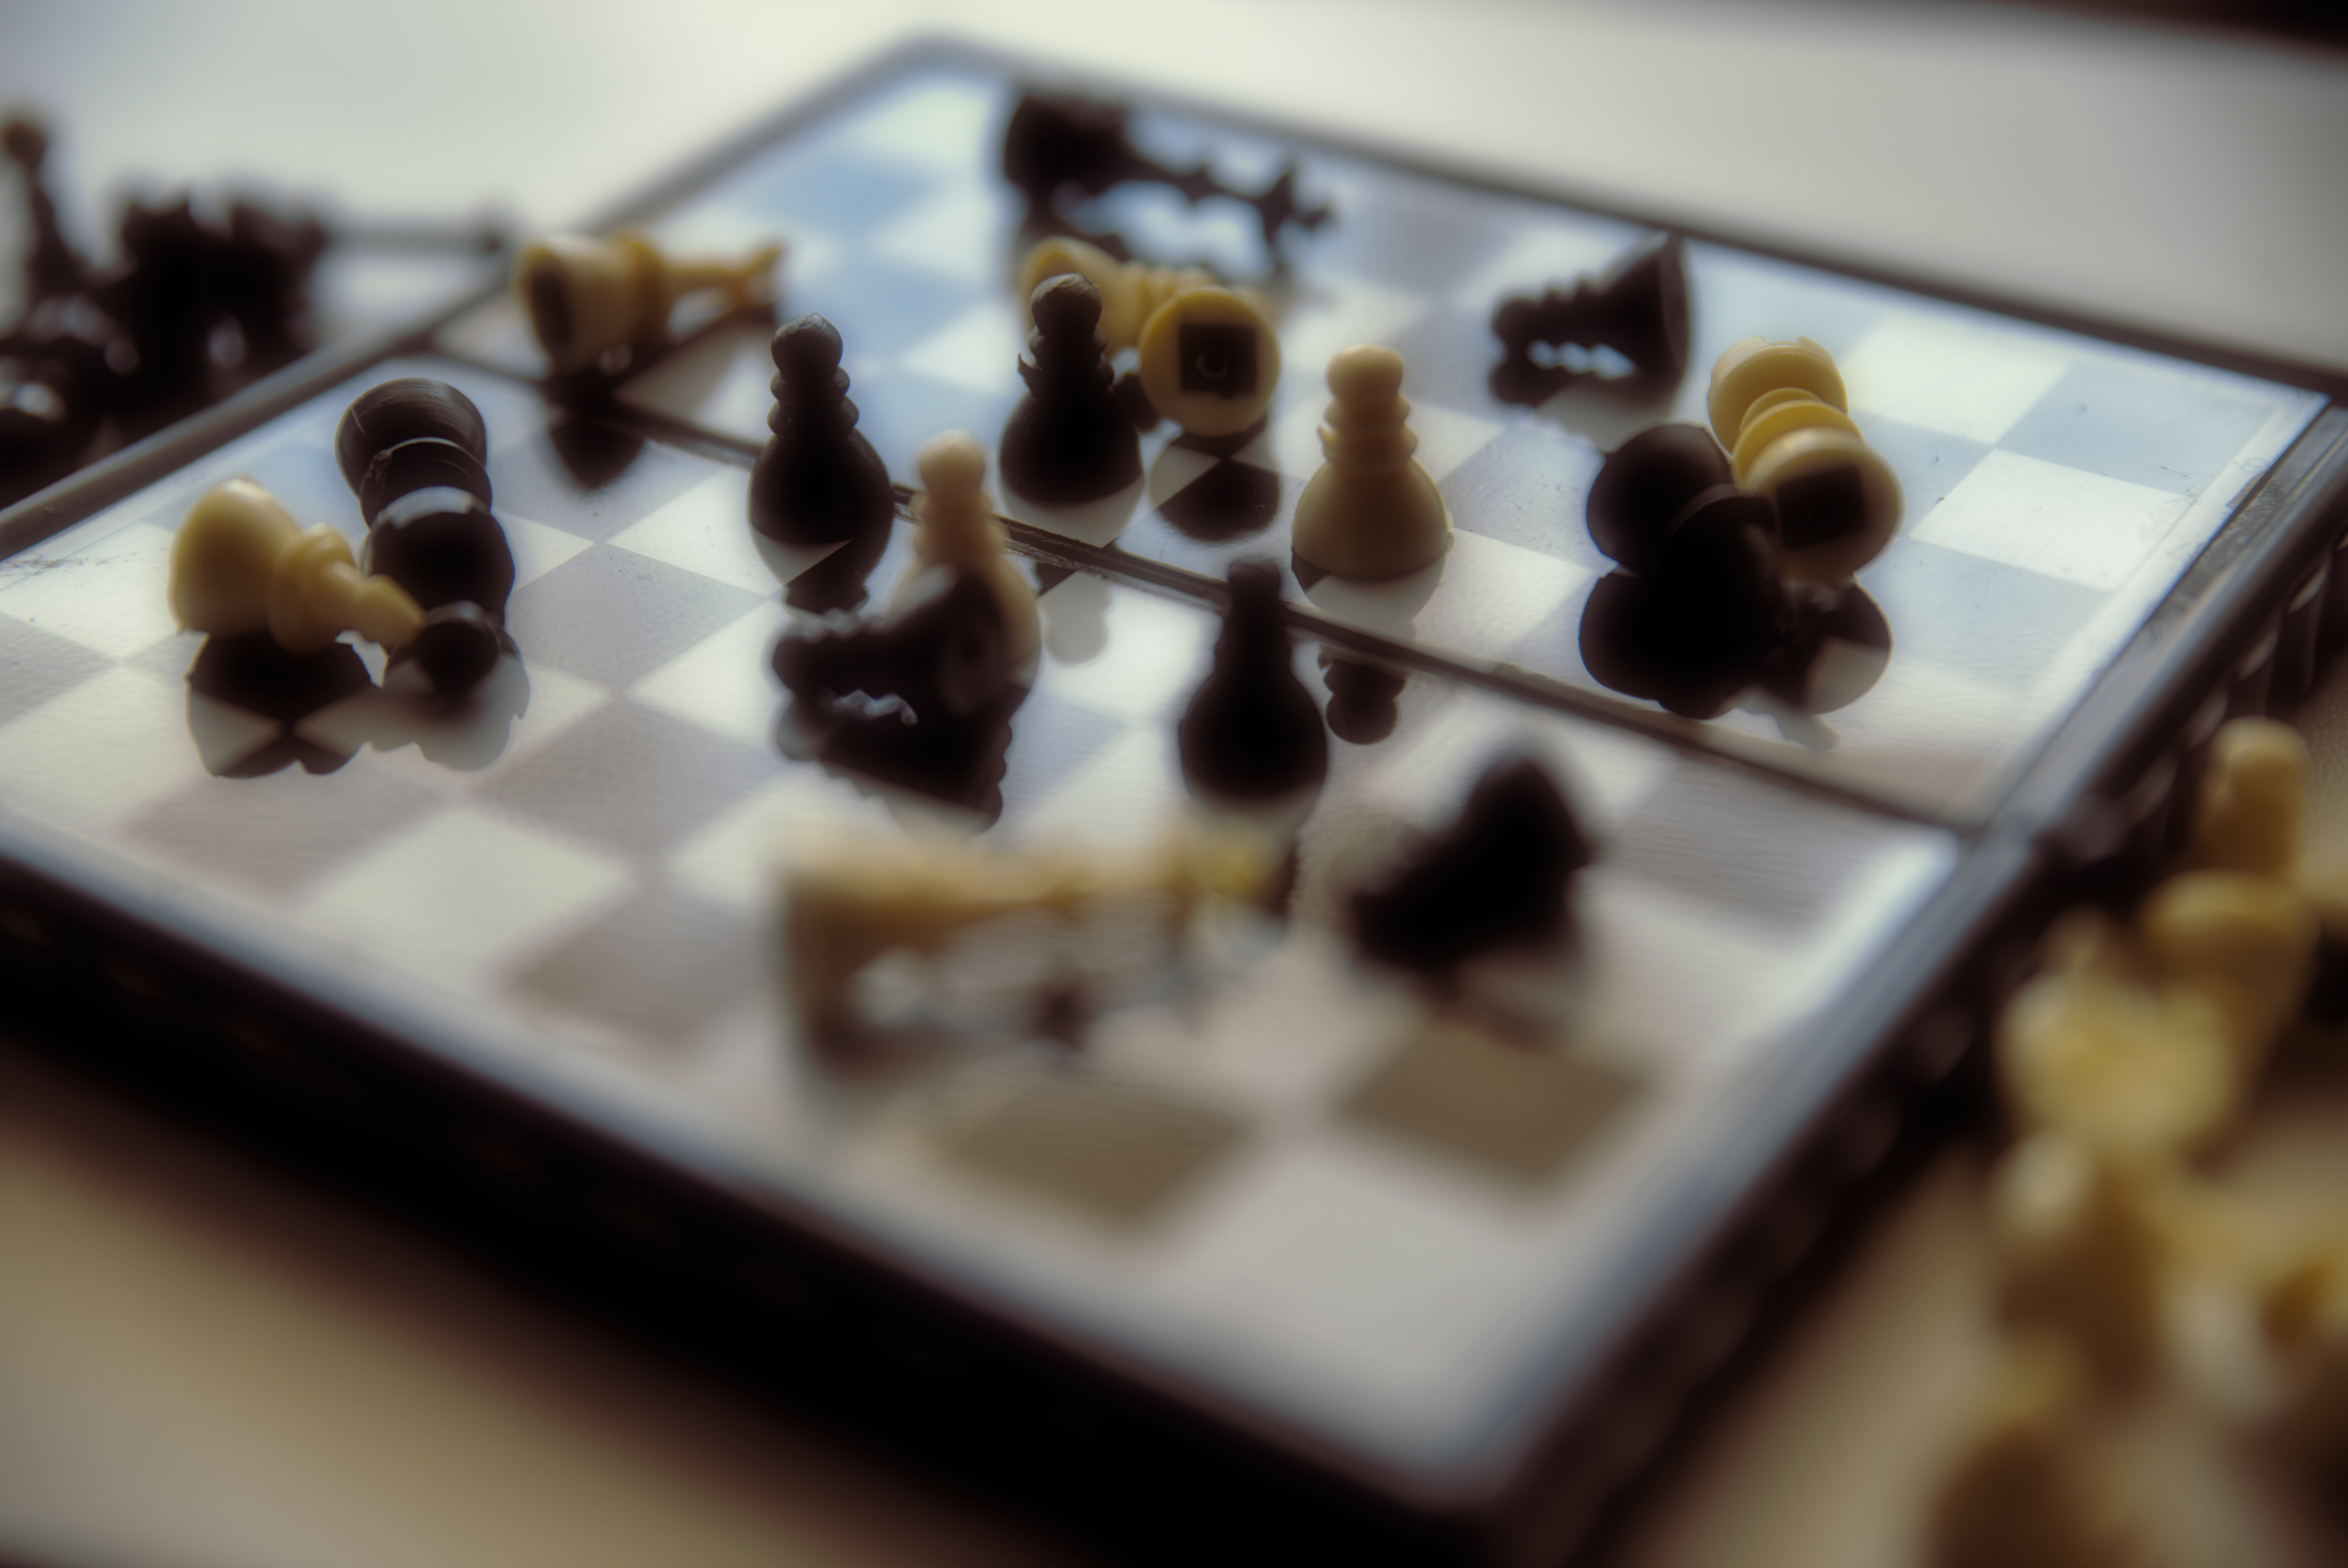
\includegraphics[width=0.8\textwidth, keepaspectratio=true]{crochess.jpg} \\ [2.0cm]

    \hspace{2.5mm} \textbf{\large{Mario Mlačak}} \\ [2.0cm]
\end{center} % 2.5mm == left and right margin difference
\vspace{\stretch{1}}
\end{titlepage}
% ---------------------------------------------------------- Title page

% Empty page ----------------------------------------------------------
\thispagestyle{empty}
\vspace*{0.1\textheight}
\clearpage % ..........................................................
% ---------------------------------------------------------- Empty page

% Dedication page -----------------------------------------------------
\thispagestyle{empty}
\vspace*{0.2\textheight}
\hfill{Dedicated to Miranda.}
\clearpage % ..........................................................
% ----------------------------------------------------- Dedication page

% Publisher page ------------------------------------------------------
\thispagestyle{empty}
\vspace*{0.7\baselineskip}
\begin{center}
    \emph{Mario Mlačak} \\
    \textbf{Croatian chess} \\
    and other variants \\ [2.0em]

    \emph{Copyright} \\
    Copyright \copyright \hspace{0.2ex} 2009 -- 2021 Mario Mlačak \\
    \href{mailto:mmlacak@gmail.com}{mmlacak@gmail.com} \\ [2.0em]

    \emph{Source} \\
    \href{https://github.com/mmlacak/crochess}{https://github.com/mmlacak/crochess} \\
    Version: 20241003.022425 \\ [2.0em] % book-new-commit-version-squished-utc-date-time-place-marker

    \emph{Legal} \\
    This book is published as Public Domain work, \\
    under CC0 1.0 Universal Public Domain Dedication. \\
    \href{https://en.wikipedia.org/wiki/Public\_domain}{https://en.wikipedia.org/wiki/Public\_domain} \\
    \href{https://creativecommons.org/publicdomain/zero/1.0/}{https://creativecommons.org/publicdomain/zero/1.0/} \\ [2.0em]

    \emph{Third, revised edition} \\
    2024-10-03 \\ % book-new-commit-version-date-place-marker
    Zagreb, Croatia

    \vfill
    
\includegraphics[height=1.0\baselineskip, keepaspectratio=true]{CC0_button.svg.png}
    \vspace*{0.7\baselineskip}
\end{center}
\clearpage % ..........................................................
% ------------------------------------------------------ Publisher page

% Inner title page ----------------------------------------------------
\thispagestyle{empty}
\vspace*{7.3\baselineskip}
\begin{center}
    \textbf{\Large{Croatian chess}} \\ [1.0em]
    \large{and other variants} \\ [1.0em]
    \small{3rd, revised edition} \\ [2.0cm]
    \vspace*{7.3\baselineskip}

    \textbf{\large{Mario Mlačak}} \\ [1.0em]
    \small{2024-10-03} \\ [0.5em] % book-new-commit-version-date-small-place-marker
    \small{Zagreb, Croatia}
\end{center}
\clearpage % ..........................................................
% ---------------------------------------------------- Inner title page

% Empty page ----------------------------------------------------------
\thispagestyle{empty}
\vspace*{0.1\textheight}
\clearpage % ..........................................................
% ---------------------------------------------------------- Empty page

% Gratitude page ------------------------------------------------------
\thispagestyle{empty}
\vspace*{0.2\textheight}
\begin{flushright}
My most sincere gratitude to:

Valentina Štefanić \\
Kristina Mlačak \\
Ana Mlačak

and many, many others.

Thank you all.
\end{flushright}
\clearpage % ..........................................................
% ------------------------------------------------------ Gratitude page

% Empty page ----------------------------------------------------------
\thispagestyle{empty}
\vspace*{0.1\textheight}
\clearpage % ..........................................................
% ---------------------------------------------------------- Empty page

% Introduction chapter ------------------------------------------------

% Introduction chapter ------------------------------------------------
\chapter*{Introduction}
\addcontentsline{toc}{chapter}{Introduction}

\begin{flushright}
\parbox{0.6\textwidth}{
\emph{Life's too short for chess. \\
\hspace*{\fill}{\textperiodcentered \textperiodcentered \textperiodcentered \hspace*{0.2em} Henry James Byron} } }
\end{flushright}

\noindent
I was in my aunt's house, on the border of a small village.
Through window walled garden was visible just behind the house.
Behind it was small brook. And hills in the distance. Afternoon
Sun was casting its orange rays into warm room. It was frosty
outside.

My cousin approached me with some nifty gizmo. He was a
few years older then me and was already going to school.

\noindent
"Here, look at what I got." \\
\hspace*{\fill}"What's that?" \\
"Chess set. Wanna try? Lemme show you." \\
\hspace*{\fill}"Sure."

It was small plasticky, fiddly thing designed to fit into winter's
coat pocket, to be used on the go. Folding board was also used to
hold all pieces in it. Each piece was as small as humanely usable.
Each field had a hole in the middle. Below each piece was small rod
fitting into those holes. It was colored all in red and ivory.

Short lesson revealed it's not that difficult to grasp what's going
on. Within minutes I picked it up. First match was, predictably, a
complete disaster. On the second go my cousin forgot about a piece,
and I grabbed his Queen gleefully. He surrendered.

After he left me with a new widget, I was intrigued. I wasn't
about playing the game, though. I was more into redesign it. Could it
be made better, more challenging, or just different?

\noindent
'Why not make Knight jump longer, say 3 by 1 fields?' \\
'Hmmmm...' \\
'Nah, that would make jump too long for such a small board.'

Outside, the Sun was shining red.

\clearpage % ..........................................................
% ------------------------------------------------ Introduction chapter

% ------------------------------------------------ Introduction chapter

% Prerequisites chapter -----------------------------------------------

% Prerequisites chapter -----------------------------------------------
\chapter*{Prerequisites}
\addcontentsline{toc}{chapter}{Prerequisites}

\begin{flushright}
\parbox{0.7\textwidth}{
\emph{It does not matter how slowly you go as long as you do not stop. \\
\hspace*{\fill}{\textperiodcentered \textperiodcentered \textperiodcentered \hspace*{0.2em} Confucius} } }
\end{flushright}

\noindent
This document describes new variants of chess, new pieces and rules. In this document I'll describe only
even variants. For details on odd variants see 'Odd variants' in the Appendix.

\textbf{\huge{TODO :: FIX ME !!!}} % TODO :: FIX ME !!!

In this document I'm assuming you have the complete prior knowledge of classical chess pieces and rules.
If not, please visit Wikipedia entry on this subject at: \\
\href{https://en.wikipedia.org/wiki/Rules\_of\_chess}{https://en.wikipedia.org/wiki/Rules\_of\_chess}.

In this book, I use term move defined as one player's complete move. For details see chapter 'Terms' in
Appendix.

\clearpage
% ----------------------------------------------- Prerequisites chapter

% ----------------------------------------------- Prerequisites chapter

% Classical Game chapter ----------------------------------------------

% Copyright (c) 2015 - 2019 Mario Mlačak, mmlacak@gmail.com
% Published as Public Domain work, under CC0 1.0 Universal Public Domain Dedication. See LICENSING, COPYING files for details.

% Classical Chess -----------------------------------------------------
\chapter*{Classical Chess}
\addcontentsline{toc}{chapter}{Classical Chess}
\label{ch:Classical Chess}

\begin{flushright}
\parbox{0.8\textwidth}{
\emph{A great war leaves the country with three armies -
an army of cripples, an army of mourners, and an army of thieves. \newline
\hspace*{\fill}{\textperiodcentered \textperiodcentered \textperiodcentered \hspace*{0.2em} German proverb} } }
\end{flushright}

\noindent
About Classical Chess is written really everything already, and I have
nothing to add, except to use it as an example on how to read the book.

\clearpage % ..........................................................
% Pieces **************************************************************

\section*{Pieces}
\addcontentsline{toc}{section}{Pieces}
\label{sec:Classical Chess/Pieces}

The easiest way to introduce readers to the rendering of classical pieces
is to show chessboard with initial setup:

\noindent
\begin{figure}[!h]
\includegraphics[width=1.0\textwidth, keepaspectratio=true]{boards/02_classical.png}
\caption{Classical Chess, initial setup}
\label{fig:02_classical}
\end{figure}

\noindent
You can compare this with official rendering at \algfmt{FIDE~2.3}.

\clearpage % ..........................................................

\subsection*{Bishop}
\addcontentsline{toc}{subsection}{Bishop}
\label{sec:Classical Chess/Pieces/Bishop}

\noindent
\begin{wrapfigure}[12]{l}{0.4\textwidth}
\centering
\includegraphics[width=0.4\textwidth, keepaspectratio=true]{pieces/bishop/02_classical.png}
\caption{Bishop}
\label{fig:bishop/02_classical}
\end{wrapfigure}
New pieces are introduced with zoomed-in image, on a \mbox{2 $\times$ 2} board.
Light pieces are rendered on a lower row, dark pieces are on an upper row,
regardless of actual colors used in a particular variant. % \newline
% \indent

Light fields are always in lower-right and upper-left corner, while dark fields
are always in lower-left and upper-right corner, regardless which actual colors
are used to paint board.

% ************************************************************** Pieces
% \clearpage % ..........................................................
% Chessboard **********************************************************

\section*{Chessboard}
\addcontentsline{toc}{section}{Chessboard}
\label{sec:Classical Chess/Chessboard}

As seen on the chessboard on previous page, light player starts from bottom of
a chessboard, while dark player starts from top. This arrangement is used by FIDE
(see \algfmt{FIDE~2.3}), and also for all the examples in this book, and for all
new variants, regardless the size of a chessboard used in a variant.

In such a setup, color of lower-right (and upper-left) corner are determined by
FIDE to be light colored, see \algfmt{FIDE~2.1}; this also applies to all new
variants, regardless which actual colors are used to paint chessboards.

In FIDE handbook, and elsewhere, chessboard is said to be made of \mbox{8 $\times$ 8}
grid of squares; in this book squares are referred to as fields.

\clearpage % ..........................................................
% Examples ============================================================

\subsection*{Examples}
\addcontentsline{toc}{subsection}{Examples}
\label{sec:Classical Chess/Chessboard/Examples}

\vspace*{-0.7\baselineskip}
\noindent
\begin{wrapfigure}[12]{l}{0.4\textwidth}
\centering
\includegraphics[width=0.4\textwidth, keepaspectratio=true]{examples/02_c/scn_cc_01_rook_not_blocked.png}
\vspace*{-1.4\baselineskip}
\caption{Rook not blocked}
\label{fig:scn_cc_01_rook_not_blocked}
\end{wrapfigure}
Some examples are not showing whole chessboard; often, those examples also
feature partial fields around sides to convey which part of chessboard has
been depicted. \newline
\indent
Here, we have hints of fields upwards and to the right, so example shows
lower-left corner of a chessboard. \newline
\indent
Green arrow is used in cases where move is legal, but there is nothing special
about it.

\vspace*{2.7\baselineskip}
\noindent
\begin{wrapfigure}[14]{l}{0.4\textwidth}
\centering
\includegraphics[width=0.4\textwidth, keepaspectratio=true]{examples/02_c/scn_cc_02_rook_blocked.png}
\vspace*{-1.4\baselineskip}
\caption{Rook blocked}
\label{fig:scn_cc_02_rook_blocked}
\end{wrapfigure}
In previous example, light Rook simply going forward (towards opponent's initial
positions) was shown with only a single arrow, as it would be in FIDE handbook and
elsewhere. \newline
\indent
In this book all examples shows individual steps as arrows, as movement can be
blocked at any field which a piece visits. All fields that can be visited are
called step-fields. \newline
\indent
Grey arrows are used when movement is otherwise legal, but a piece cannot move
since it's e.g. blocked by own other piece.

\clearpage % ..........................................................

\vspace*{-1.4\baselineskip}
\noindent
\begin{wrapfigure}[8]{l}{0.4\textwidth}
\centering
\includegraphics[width=0.4\textwidth, keepaspectratio=true]{examples/02_c/scn_cc_03_rook_capturing.png}
\vspace*{-1.4\baselineskip}
\caption{Rook capturing}
\label{fig:scn_cc_03_rook_capturing}
\end{wrapfigure}
Fields where a piece can capture opponent's piece are called capture-fields;
these are often the same as step-fields. \newline
\indent
Blue arrows are used mostly when some action is performed by a piece beside just
moving, like e.g. capturing opponent's piece.

\vspace*{6.7\baselineskip}
\noindent
\begin{wrapfigure}[13]{l}{0.4\textwidth}
\centering
\includegraphics[width=0.4\textwidth, keepaspectratio=true]{examples/02_c/scn_cc_04_rook_diagonal.png}
\vspace*{-1.4\baselineskip}
\caption{Rook going diagonally}
\label{fig:scn_cc_04_rook_diagonal}
\end{wrapfigure}
Red arrows are used for movement that is illegal depending on context, either
in all cases, or just in a current example. \newline
\indent
Here, light Rook cannot make step to the right after it has already taken step
upwards.

Colors of arrows are not tied to a singular purpose, there are occasions when
colors are used just to draw attention to a particular step, or (rarely) just
to differentiate between each other.

% ============================================================ Examples
% ********************************************************** Chessboard
\clearpage % ..........................................................

\noindent
\TODO :: introduction \newline

\noindent
\textrightarrow basic terminology: turn, move, cycle, figure, ... \newline
\textrightarrow new terminology: rush, steps, step-fields, capture-fields \newline
\textrightarrow conflicting terminology: activating a piece, ply (?) \newline

\noindent
\textrightarrow arrows \& colors \newline
\textrightarrow markers, texts (enumerations vs. labels) \newline
\textrightarrow navigation \newline

\noindent
\textrightarrow context, exceptions \newline

\clearpage % ..........................................................
% ----------------------------------------------------- Classical Chess

% ---------------------------------------------- Classical Game chapter

% Croatian Ties chapter -----------------------------------------------

% Croatian Ties chapter -----------------------------------------------
\chapter*{Croatian Ties}
\addcontentsline{toc}{chapter}{Croatian Ties}

\begin{flushright}
\parbox{0.7\textwidth}{
\emph{Secrecy is the first essential in affairs of the State. \\
\hspace*{\fill}{\textperiodcentered \textperiodcentered \textperiodcentered \hspace*{0.2em} De Richelieu} } }
\end{flushright}

\noindent
Croatian Ties is chess variant which is played on 10 x 10 board,
with silver and red fields and dark silver and dark red pieces.
In algebraic notation, columns are enumerated from 'a' to 'j',
and rows are enumerated from '1' to '10'. A new piece is
introduced, Pegasus.

\clearpage % ..........................................................

\section*{Pegasus}
\addcontentsline{toc}{section}{Pegasus}

\noindent
\begin{wrapfigure}[9]{l}{0.4\textwidth}

\includegraphics[width=0.4\textwidth, keepaspectratio=true]{pieces/07_pegasus.png}
\caption{Pegasus}
\label{fig:pegasus}
% % \centering
\end{wrapfigure}
Pegasus moves similarly to Knight, but it can continue its jumpy movement
until another piece is encountered, or it runs out of board. Note that once
in movement, Pegasus can not change its' heading.

Pegasus symbol in algebraic notation is 'G', to avoid confusion with Pawn.

\vspace{2\baselineskip}
\subsection*{Step-fields}
\addcontentsline{toc}{subsection}{Step-fields}

\noindent
\begin{wrapfigure}[15]{l}{0.5\textwidth}
\includegraphics[width=0.5\textwidth, keepaspectratio=true]{examples/04_move_pegasus_initial.png}
\caption{Pegasus initial step}
\label{fig:pegasus_initial_step}
% % \centering
\end{wrapfigure}
In the example on the left we have Pegasus with all valid initial moves marked.
These all are the same as valid moves for Knight. Pegasus' movement is not hampered
by piece if it's placed on any unmarked field. Pegasus can "jump" over it just as
Knight would.

\clearpage % ..........................................................

\noindent
% \begin{figure}[t]
\begin{figure}[!t]
\includegraphics[width=1.0\textwidth, keepaspectratio=true]{examples/04_move_pegasus_direction.png}
\caption{Pegasus move direction}
\label{fig:pegasus_move_direction}
% \centering
\end{figure}
Once direction is chosen Pegasus can continue its' movement performing one jump
after another in order from nearest field to furthest. Here, this is marked
with green arrows. Accessible fields are marked 1 to 4, in order of accessibility,
from nearest to furthest. Again, once direction is chosen it can't be changed anymore.
For instance, after reaching field 2 it's not allowed to change direction to 2f (or
any other greyed-out arrow).

\clearpage % ..........................................................

\noindent
% \begin{figure}[t]
\begin{figure}[!t]
\includegraphics[width=1.0\textwidth, keepaspectratio=true]{examples/04_move_pegasus.png}
\caption{Pegasus moves}
\label{fig:pegasus_moves}
% \centering
\end{figure}
Move along arrow is called step. Field at which arrow points to is called step-field.
Pegasus can "jump" over pieces on non-step-fields, Rooks in example above. Numbers
here enumerate directions of movement. Own piece on step-field stops Pegasus at
preceding step field, see direction 2. Opponent's piece on step-field can be captured.
Just as with any other piece that would finish the move, meaning Pegasus would have to
stop at captured step-field, see direction 1.

\clearpage % ..........................................................

\section*{En passant}
\addcontentsline{toc}{section}{En passant}

\noindent
\begin{wrapfigure}[18]{l}{0.4\textwidth}
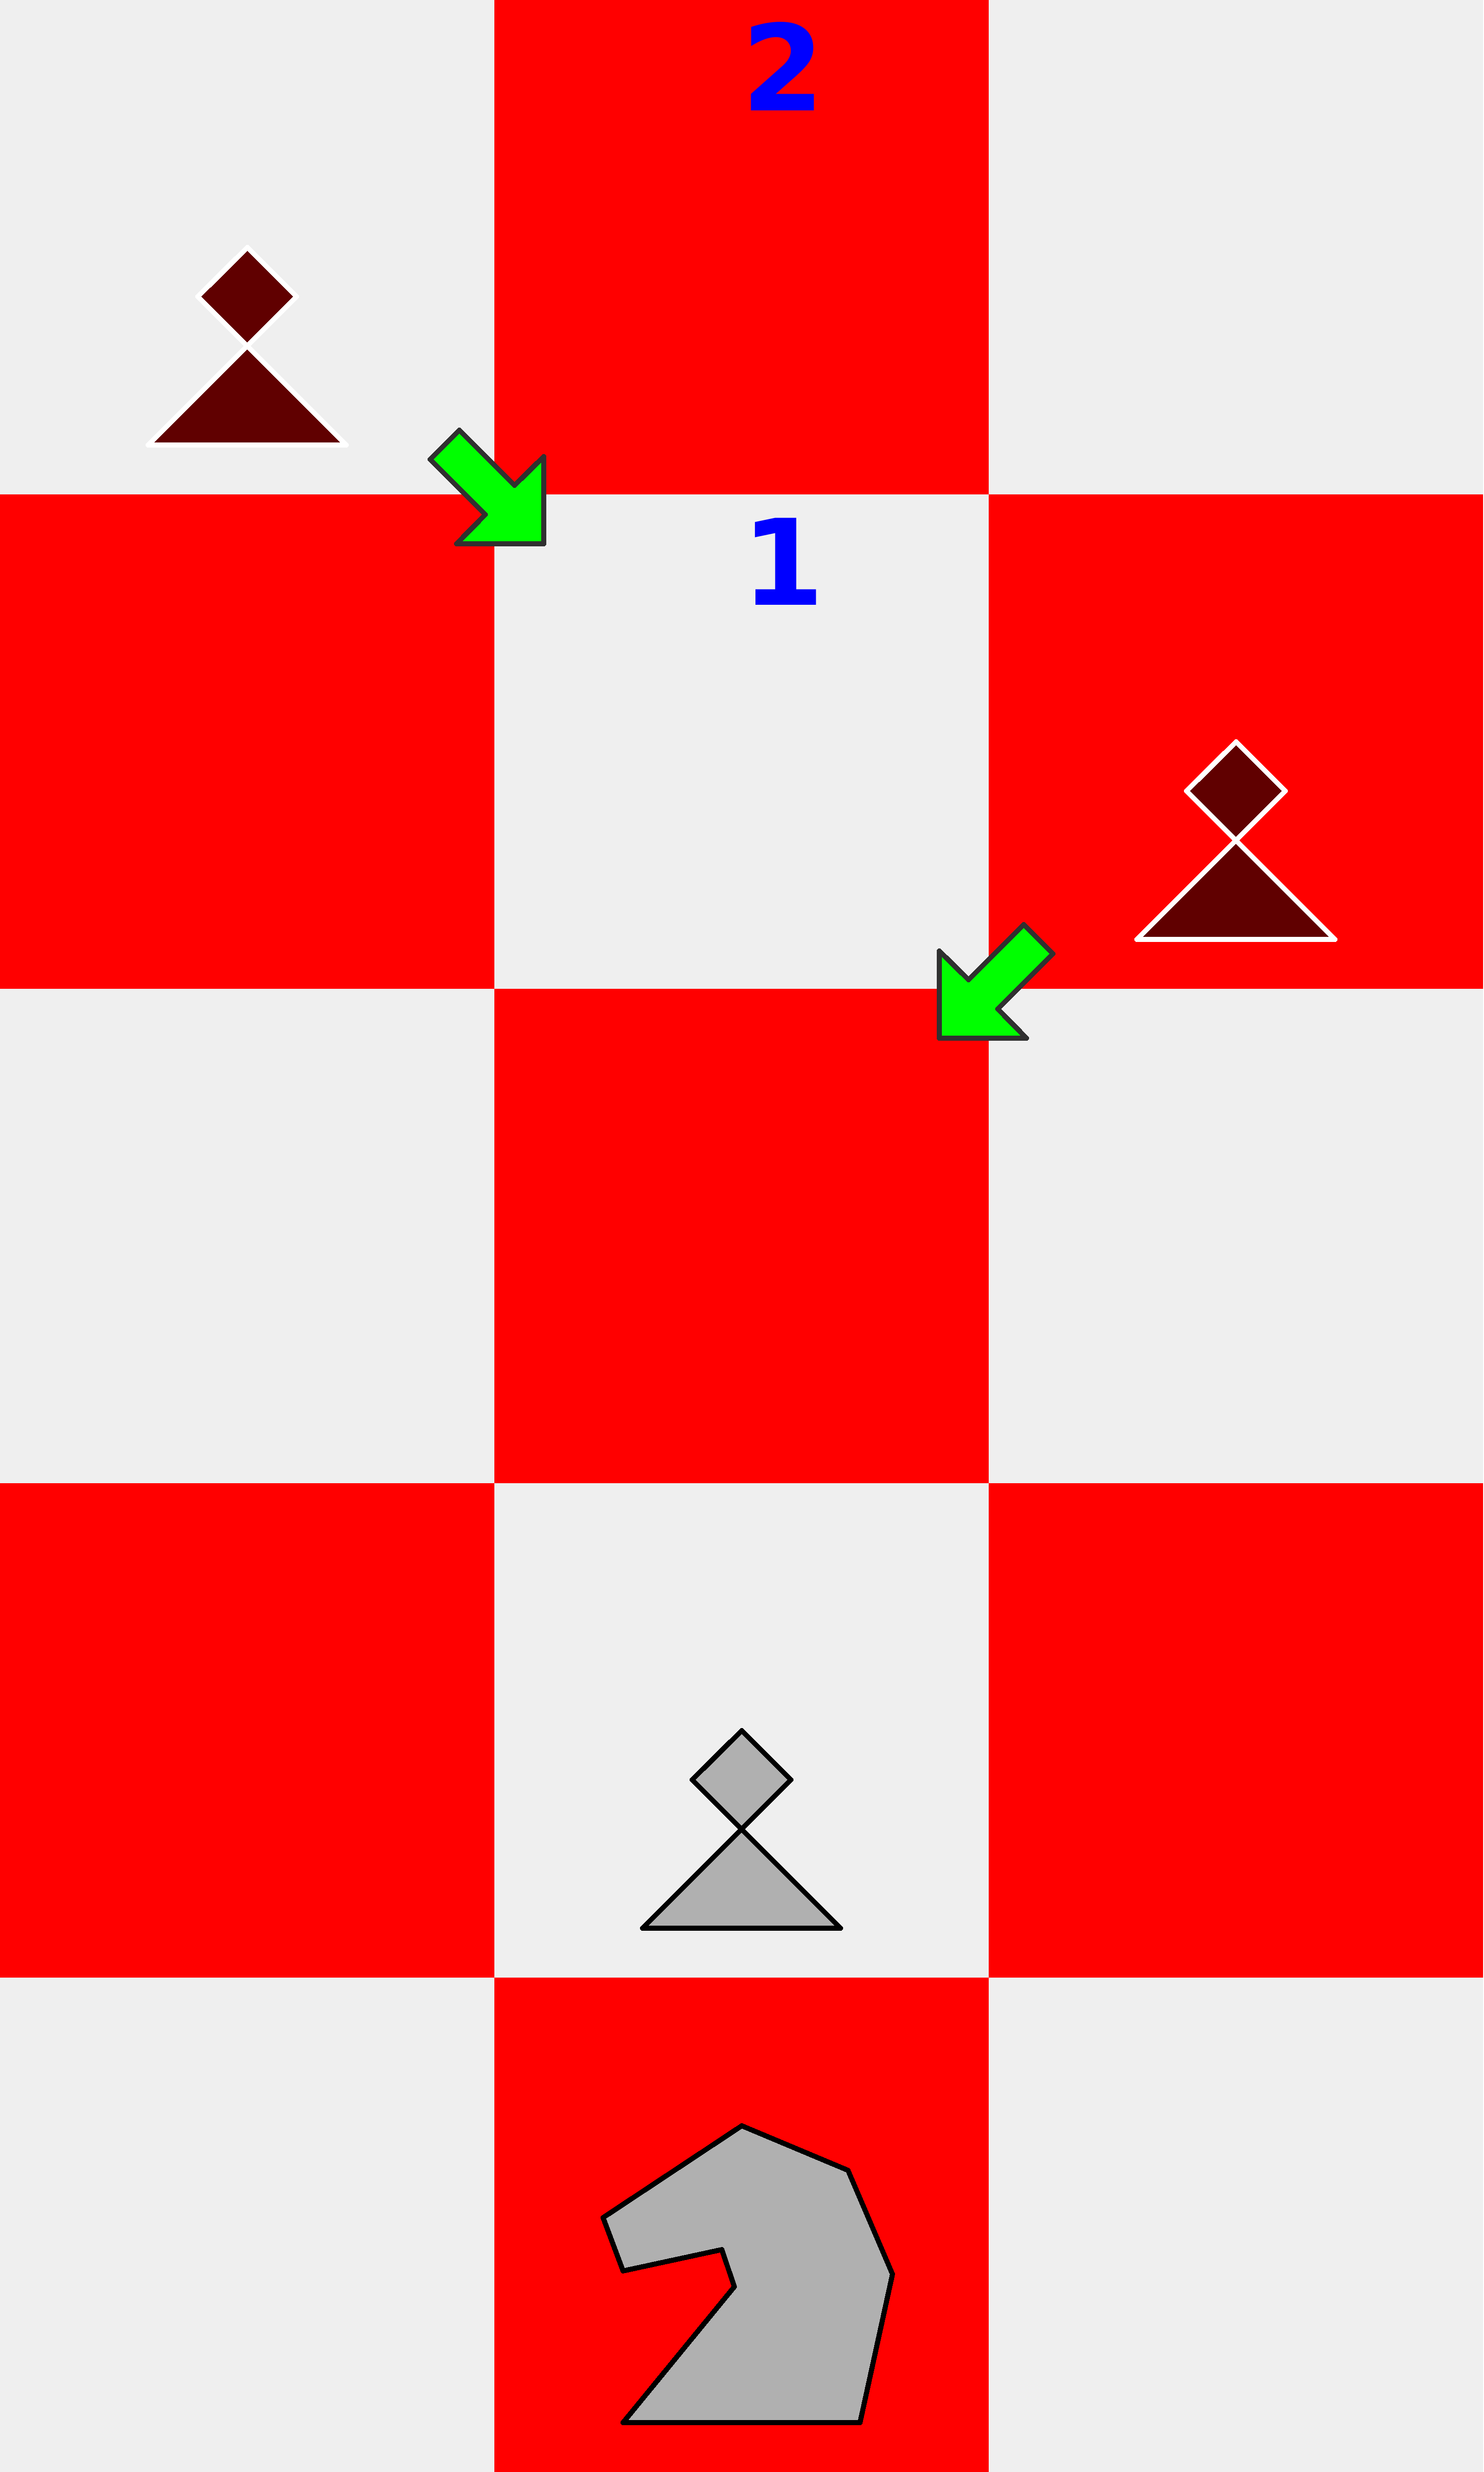
\includegraphics[width=0.4\textwidth, keepaspectratio=true]{en_passants/04_croatian_ties_en_passant.png}
\caption{En passant}
\label{fig:cc_en_passant}
% % \centering
\end{wrapfigure}
En passant is identical to one in Classic Chess, only difference is that Pawn can now
move longer on initial turn, up to 3 fields in this instance. As expected, all passed-by
opponent's Pawns also gain en passant opportunity.

Passed-by Pawns are those which had field under their attack passed over by opponent's Pawn
on its' initial turn, if that move was at least 2 fields long.

For example, on the left, if light Pawn's initial move was of maximum length both dark Pawns
would have en passant opportunity. Naturaly, if initial move was only to field marked 1, only
dark Pawn on the right would gain en passant opportunity.

\clearpage % ..........................................................

\section*{Castling}
\addcontentsline{toc}{section}{Castling}

Castling is essentially the same as it is in Classical Chess, only real difference is that
King can move either 2 or 3 fields across. All other constraints from Classical Chess still
applies, described in detail here \\
\href{https://en.wikipedia.org/wiki/Castling}{https://en.wikipedia.org/wiki/Castling}.

\noindent
\begin{figure}[!h]
% \begin{figure}[!t]

\includegraphics[width=1.0\textwidth, keepaspectratio=true]{castlings/04_croatian_ties_castling.png}
\caption{Castling}
\label{fig:cc_castling}
% \centering
\end{figure}

In example above, all valid King's castling moves are numbered. Regardless if King performs
long or short castling move, Rook would always end up on the opposite side of King on the
field immediately next to it, i.e. closer to center.

\noindent
\begin{figure}[!h]
% \begin{figure}[!t]

\includegraphics[width=1.0\textwidth, keepaspectratio=true]{castlings/long_left/04_croatian_ties_castling_long_left.png}
\caption{Castling long left}
\label{fig:cc_castling_long_left}
% \centering
\end{figure}

In this example King was castling long to the left. Initial King's position is marked with "K".
After castling is finished, left Rook ends up at field immediately on the right to the King.

\clearpage % ..........................................................

\section*{Initial setup}
\addcontentsline{toc}{section}{Initial setup}

Initial setup for Light player is (mirrored for Dark one):
\texttt{PPPPPPPPPP \\
        RGNBQKBNGR}, \\
or more conveniently, as seen in this image:

\noindent
% \begin{figure}[t]
\begin{figure}[h]
\includegraphics[width=1.0\textwidth, keepaspectratio=true]{boards/04_croatian_ties.png}
\caption{Croatian Ties board}
\label{fig:croatian_ties}
% \centering
\end{figure}

\clearpage % ..........................................................
% ----------------------------------------------- Croatian Ties chapter

% ----------------------------------------------- Croatian Ties chapter

% Mayan Ascendancy chapter --------------------------------------------

% Mayan Ascendancy chapter --------------------------------------------
\chapter*{Mayan Ascendancy}
\addcontentsline{toc}{chapter}{Mayan Ascendancy}

\begin{flushright}
\parbox{0.8\textwidth}{
\emph{The world has achieved brilliance without wisdom, power without
conscience. Our is a world of nuclear giants and ethical infants. \\
\hspace*{\fill}{\textperiodcentered \textperiodcentered \textperiodcentered \hspace*{0.2em} Omar Nelson Bradley} } }
\end{flushright}

\noindent
Mayan Ascendancy is chess variant which is played on 12 x 12 board with
yellow and blue fields and with dark yellow and dark blue pieces. In
algebraic notation, columns are enumerated from 'a' to 'l', and rows are
enumerated from '1' to '12'. A new piece is introduced, Pyramid.

\clearpage % ..........................................................

\section*{Pyramid}
\addcontentsline{toc}{section}{Pyramid}

\noindent
\begin{wrapfigure}[12]{l}{0.4\textwidth}
\centering

\includegraphics[width=0.4\textwidth, keepaspectratio=true]{pieces/08_pyramid.png}
\caption{Pyramid}
\label{fig:08_pyramid}
\end{wrapfigure}
Pyramid is passive piece, meaning it can't move on its' own, it has to be
activated first. This is done by capturing a field at which Pyramid stands
with own other piece and then move Pyramid further.

Once activated Pyramid moves similar to Rook, only real difference is that
it can move for only so many fields as piece activating it has moved, i.e.
for at most as momentum received.

\subsection*{Momentum}
\addcontentsline{toc}{subsection}{Momentum}

Momentum is count of step-fields traveled over by a piece. Pyramid receives
momentum from piece which activates it. Momentum is spent by Pyramid when
moving, one for each step-field travelled. So Pyramid can't move for more
fields than received momentum, i.e. for more than activating piece has
travelled. Momentum can't be saved for later, it is wasted when Pyramid
moves for less than received momentum.

\clearpage % ..........................................................

\subsection*{Pyramid (cont.)}
\addcontentsline{toc}{subsection}{Pyramid (cont.)}

Pyramid can't check opponent's King, and consequently can't contribute to
checkmate. Pyramid can capture all the other opponent's pieces after it has
been activated, even if it has no remaining momentum, i.e. can't move any
further.

Pyramid can also promote own Pawns on opponen't side of the board. It can
also convert any opponent's piece, except King, on own side of the board.
To do either of these things, Pyramid does not have to have any remaining
momentum, it's enough if piece in question is within reach.

Pyramid can also activate other Pyramid, and transfer remaining momentum to it.
There has to be remaining momentum, it must not be 0 for activation to be permitted.

In algebraic notation symbol for Pyramid is 'A', to avoid confusion with Pawn.

\clearpage % ..........................................................

\subsection*{Activation}
\addcontentsline{toc}{subsection}{Activation}

\noindent
\begin{figure}[!h]
% \begin{figure}[!t]
\includegraphics[width=1.0\textwidth, keepaspectratio=true]{examples/06_move_pyramid_activation_init.png}
\caption{Pyramid activation}
\label{fig:06_move_pyramid_activation_init}
% \centering
\end{figure}

Here Pegasus is about to capture field on which Pyramid stands. Note, only
step-fields are counted towards momentum. After activation Pyramid would be
limited to move at most 4 fields across, i.e. at most the momentum it received
from Pegasus.

\clearpage % ..........................................................

\noindent
\begin{figure}[!h]
% \begin{figure}[!t]
\includegraphics[width=1.0\textwidth, keepaspectratio=true]{examples/06_move_pyramid_activated.png}
\caption{Pyramid activated}
\label{fig:06_move_pyramid_activated}
% \centering
\end{figure}

Above, arrows show all possible moves by Pyramid. Just like Rook, Pyramid has to
stop before own Bishop. Pyramid can capture opponent's Knight, but can't move any
further after capture. Pyramid can also capture opponent's Bishop, despite being
barely reachable.

\clearpage % ..........................................................

\noindent
\begin{figure}[!h]
% \begin{figure}[!t]
\includegraphics[width=1.0\textwidth, keepaspectratio=true]{examples/06_move_pyramid_activation_end.png}
\caption{Pyramid activation end}
\label{fig:06_move_pyramid_activation_end}
% \centering
\end{figure}

Here, Pyramid movement ends by capturing opponent's Knight, which also ends light
player's complete move.

\clearpage % ..........................................................

\subsection*{Promotion}
\addcontentsline{toc}{subsection}{Promotion}

Pyramid can promote own Pawns, but only on opponent's side of the board.
Promotion is done by activating Pyramid which then marks Pawn for promotion
by touching either Pawn or field at which it stands. Pyramid then leaves
board as if it was captured, and Pawn is replaced by desired piece, for
instance Queen.

Both Pyramid and Pawn in question has to reside on opponent's side of the
board before promotion can take place. Piece which activates Pyramid need
not to be on opponent's side of the board.

Piece which Pawn can be promoted to is from the set of all starting pieces,
except King. This promoting-to piece is not limited to pieces already being
captured.

\clearpage % ..........................................................

\noindent
\begin{figure}[!h]
% \begin{figure}[!t]
\includegraphics[width=1.0\textwidth, keepaspectratio=true]{examples/06_move_pyramid_promo_init.png}
\caption{Promotion start}
\label{fig:06_move_pyramid_promo_init}
% \centering
\end{figure}

Here, Pegasus is accumulating momentum while travelling over step-fields. After
activation Pyramid would be limited to move at most 4 fields across, i.e. at most
the momentum it received from Pegasus.

\clearpage % ..........................................................

\noindent
\begin{figure}[!h]
% \begin{figure}[!t]
\includegraphics[width=1.0\textwidth, keepaspectratio=true]{examples/06_move_pyramid_promo_activate.png}
\caption{Promotion, Pyramid activated}
\label{fig:06_move_pyramid_promo_activate}
% \centering
\end{figure}

Above, Pegasus captured field at which Pyramid was situated, arrows now show
all possible moves by Pyramid. Pyramid can't promote Pawn 2, as it is still
located on own half of the chessboard. Just as Rook, Pyramid can't advance
past Pawn 2. Only full movement to the right leads to promotion of Pawn 1,
shown in red.

\clearpage % ..........................................................

\noindent
\begin{figure}[!h]
% \begin{figure}[!t]
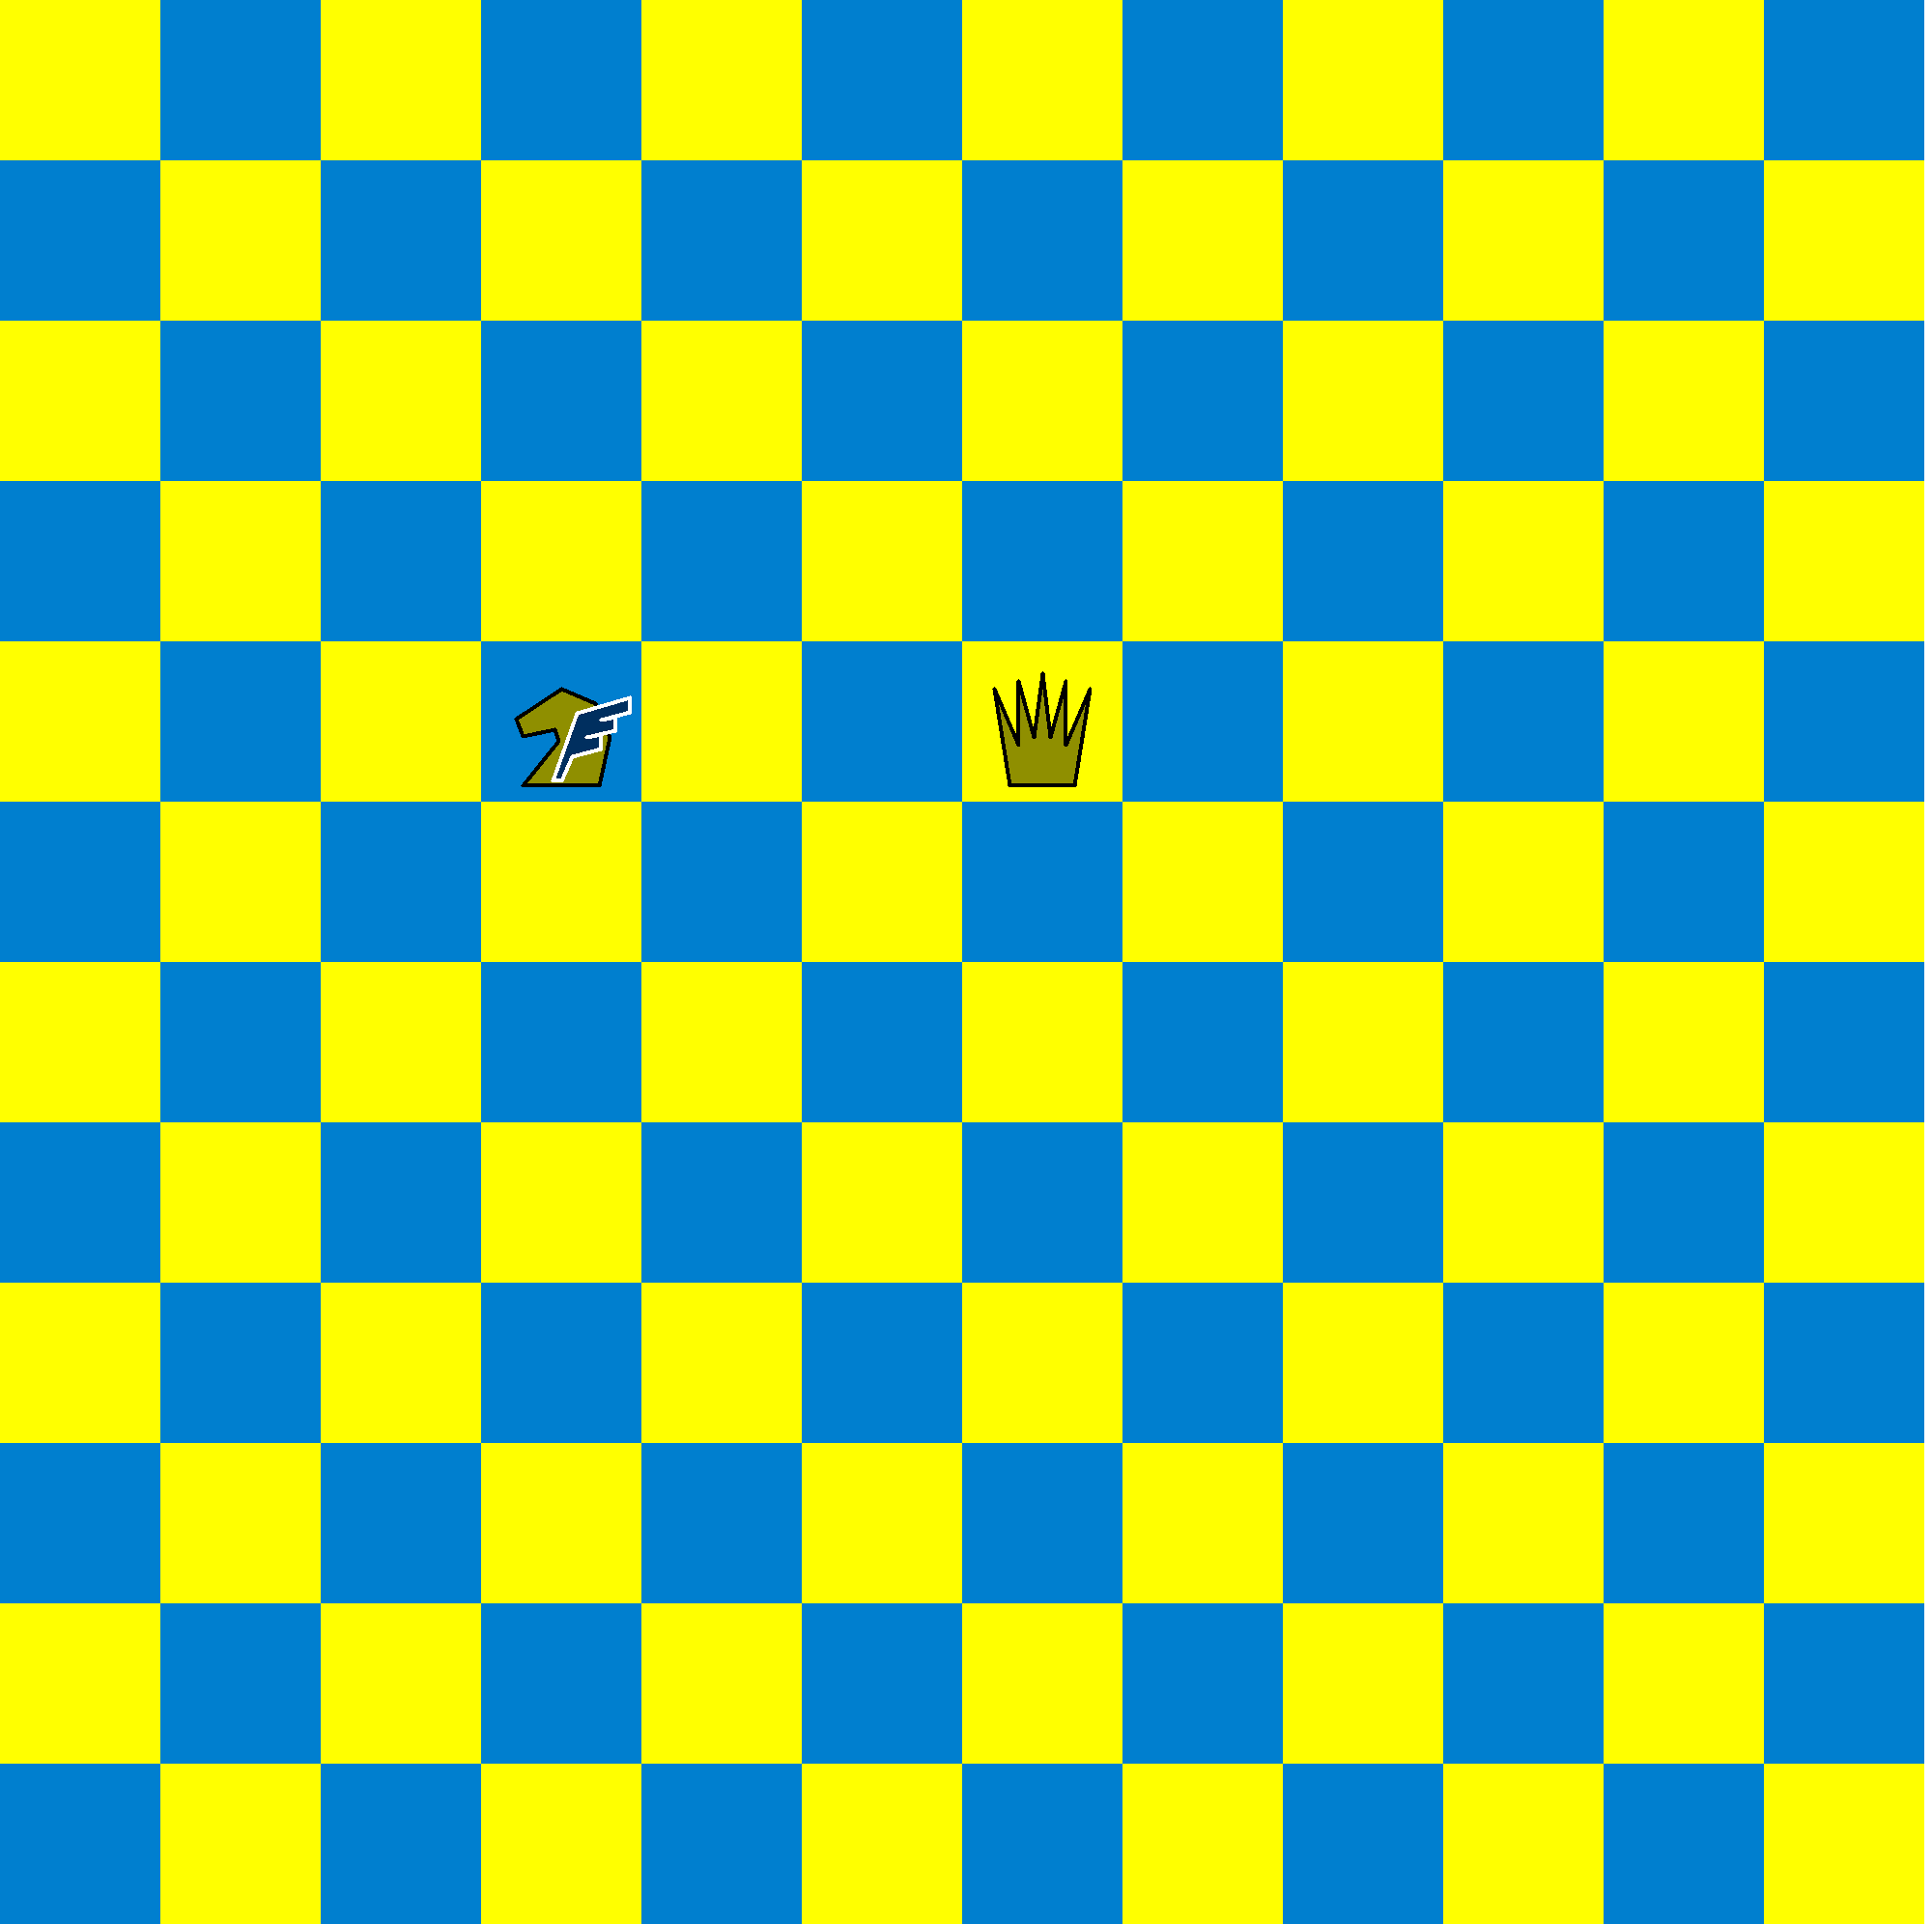
\includegraphics[width=1.0\textwidth, keepaspectratio=true]{examples/06_move_pyramid_promo_end.png}
\caption{Promotion end}
\label{fig:06_move_pyramid_promo_end}
% \centering
\end{figure}

Now that Pyramid has reached Pawn 1, it is removed from the board and piece of
choice, in this instance Queen, replaces Pawn. Just as with ordinary promotion,
this can take place regardless of which pieces has been captured, e.g. even if
own Queen is still present on chessboard.

\clearpage % ..........................................................

\subsection*{Conversion}
\addcontentsline{toc}{subsection}{Conversion}

Pyramid can convert opponent's pieces, except King, but only on own side of
the board. Conversion is done by activating Pyramid which then marks opponent's
piece for conversion by touching either piece or field at which it stands. Now
Pyramid leaves the board as if it was captured, and opponent's piece is replaced
by own piece of the same type.

Both Pyramid and opponent's piece has to reside on own side of the board
before conversion can take place. Piece which activates Pyramid need not
to be on own side of the board. As with promotion, conversion is not limited
to pieces which has been captured.

Note that Pyramid might just as well capture opponent's piece. Differences are
who leaves chessboard, and what remains on captured field. Capture itself with
Pyramid is in no way different than that with Rook. In either case, converting
or capturing, it is enough if Pyramid can reach opponent's piece, i.e. has
enough momentum from activating piece.

\clearpage % ..........................................................

\noindent
\begin{figure}[!h]
% \begin{figure}[!t]
\includegraphics[width=1.0\textwidth, keepaspectratio=true]{examples/06_move_pyramid_conversion_init.png}
\caption{Conversion start}
\label{fig:06_move_pyramid_conversion_init}
% \centering
\end{figure}

For classic pieces, step-fields are just fields which piece traveled over,
in case of Bishop above that is 4 fields. Again, that is momentum Pyramid
will receive with activation and limits how far it could move afterwards.

\clearpage % ..........................................................

\noindent
\begin{figure}[!h]
% \begin{figure}[!t]
\includegraphics[width=1.0\textwidth, keepaspectratio=true]{examples/06_move_pyramid_conversion_activated.png}
\caption{Conversion, Pyramid activated}
\label{fig:06_move_pyramid_conversion_activated}
% \centering
\end{figure}

Above, Bishop captured field at which Pyramid was situated, arrows now show
all possible moves by Pyramid. Pyramid can't convert opponent's Bishop, as it
is still located on own side of chessboard. Again, just like Rook, Pyramid
can't advance past opponent's Bishop. Only full movement to the right leads
to conversion of opponent's Rook, shown in red.

\clearpage % ..........................................................

\noindent
\begin{figure}[!h]
% \begin{figure}[!t]
\includegraphics[width=1.0\textwidth, keepaspectratio=true]{examples/06_move_pyramid_conversion_end.png}
\caption{Conversion end}
\label{fig:06_move_pyramid_conversion_end}
% \centering
\end{figure}

Now that Pyramid has reached opponent's Rook, it is removed from the board and
own Rook replaces opponent's Rook. This conversion can still take place, regardless
if any light Rook has been captured or not, i.e. even with both light Rooks still
present on chessboard. Capturing opponent's Rook would simply leave Pyramid in
place of it.

\clearpage % ..........................................................

\subsubsection*{Converting opponent's Rook}
\addcontentsline{toc}{subsubsection}{Converting opponent's Rook}

\noindent
\begin{figure}[!h]
% \begin{figure}[!t]
\includegraphics[width=1.0\textwidth, keepaspectratio=true]{examples/06_move_pyramid_conversion_rook_init.png}
\caption{Converting opponent's Rook}
\label{fig:06_move_pyramid_conversion_rook_init}
% \centering
\end{figure}

Converting opponent's Rook in an initial position of own Rook grants them ability
to castle.

\noindent
\begin{figure}[!h]
% \begin{figure}[!t]
\includegraphics[width=1.0\textwidth, keepaspectratio=true]{examples/06_move_pyramid_conversion_rook_end.png}
\caption{Possible castling fields}
\label{fig:06_move_pyramid_conversion_rook_end}
% \centering
\end{figure}

King can now castle to any numbered field. Rook would be moved onto the inner field,
next to the King.

\noindent
\begin{figure}[!h]
% \begin{figure}[!t]
\includegraphics[width=1.0\textwidth, keepaspectratio=true]{examples/06_move_pyramid_conversion_rook_castling.png}
\caption{Castling performed}
\label{fig:06_move_pyramid_conversion_rook_castling}
% \centering
\end{figure}

To actually perform castling, in the next move or at some point later, all the other
requirements for castling has to be satisfied, with Rook prohibited to move after
conversion.

\clearpage % ..........................................................

\subsubsection*{Converting opponent's Pawn}
\addcontentsline{toc}{subsubsection}{Converting opponent's Pawn}

\noindent
\begin{wrapfigure}[8]{l}{0.6\textwidth}
\centering
\includegraphics[width=0.25\textwidth, keepaspectratio=true]{examples/06_move_pyramid_conversion_pawn_init.png}
\caption{Converting opponent's Pawn}
\label{fig:06_move_pyramid_conversion_pawn_init}
\end{wrapfigure}
Converting opponent's Pawn in an initial position of own Pawn grants them
ability to be rushed, and subjects them to opponent's en-passant move.

\vspace*{0.2\textheight}
\noindent
\begin{wrapfigure}{l}{0.6\textwidth}
\centering
\includegraphics[width=0.25\textwidth, keepaspectratio=true]{examples/06_move_pyramid_conversion_pawn_end.png}
\caption{Possible initial movement}
\label{fig:06_move_pyramid_conversion_pawn_end}
\end{wrapfigure}
In this example dark Pawn would have en passant opportunity, should converted
light Pawn be rushed to any numbered field.

\clearpage % ..........................................................

\subsection*{Cascading}
\addcontentsline{toc}{subsection}{Cascading}

\noindent
\begin{figure}[!h]
% \begin{figure}[!t]
\includegraphics[width=1.0\textwidth, keepaspectratio=true]{examples/06_move_pyramid_cascading_init.png}
\caption{Cascading start}
\label{fig:06_move_pyramid_cascading_init}
% \centering
\end{figure}

Once activated, Pyramid can also activate another Pyramid. To do so, activated
Pyramid has to have at least 1 remaining momentum to transfer it to another
Pyramid. If all momentum received was spent moving, Pyramid cannot activate
another Pyramid.

\clearpage % ..........................................................

\noindent
\begin{figure}[!h]
% \begin{figure}[!t]
\includegraphics[width=1.0\textwidth, keepaspectratio=true]{examples/06_move_pyramid_cascading_activated_1.png}
\caption{Cascading, 1st Pyramid activated}
\label{fig:06_move_pyramid_cascading_activated_1}
% \centering
\end{figure}

Pyramid 1 has been activated by Queen and received momentum of 5, arrows now show
its' all possible moves. Note, Pyramid 3 can't be activated, it's on the very end
of fields reachable by Pyramid 1.

\clearpage % ..........................................................

\noindent
\begin{figure}[!h]
% \begin{figure}[!t]
\includegraphics[width=1.0\textwidth, keepaspectratio=true]{examples/06_move_pyramid_cascading_activated_2.png}
\caption{Cascading, 2nd Pyramid activated}
\label{fig:06_move_pyramid_cascading_activated_2}
% \centering
\end{figure}

Pyramid 2 has been activated by Pyramid 1 and in the process received momentum of 2,
arrows now show all possible moves by Pyramid 2.

\clearpage % ..........................................................

\noindent
\begin{figure}[!h]
% \begin{figure}[!t]
\includegraphics[width=1.0\textwidth, keepaspectratio=true]{examples/06_move_pyramid_cascading_end.png}
\caption{Cascading end}
\label{fig:06_move_pyramid_cascading_end}
% \centering
\end{figure}

Pyramid 2 has finished its' movement, and so it ends light player's complete move.

\clearpage % ..........................................................

\subsection*{Against King}
\addcontentsline{toc}{subsection}{Against King}

Pyramid can't check opponent's King, meaning that King is not under attack
even if Pyramid could capture any other piece on the same field.

\noindent
\begin{figure}[!h]
% \begin{figure}[!t]
\includegraphics[width=1.0\textwidth, keepaspectratio=true]{examples/06_move_pyramid_vs_king.png}
\caption{Pyramid vs. King}
\label{fig:06_move_pyramid_vs_king}
% \centering
\end{figure}

Above, King is not under attack from Pyramid.

\noindent
\begin{figure}[!h]
% \begin{figure}[!t]
\includegraphics[width=1.0\textwidth, keepaspectratio=true]{examples/06_move_pyramid_vs_bishop.png}
\caption{Pyramid vs. Bishop}
\label{fig:06_move_pyramid_vs_bishop}
% \centering
\end{figure}

Bishop in the same place, however, could be captured without any hindrance.

\clearpage % ..........................................................

\subsection*{Activation by Pawn}
\addcontentsline{toc}{subsection}{Activation by Pawn}

\noindent
\begin{figure}[!h]
% \begin{figure}[!t]
\includegraphics[width=1.0\textwidth, keepaspectratio=true]{examples/06_move_pyramid_activation_by_pawn.png}
\caption{Pyramid activation by Pawns}
\label{fig:06_move_pyramid_activation_by_pawn}
% \centering
\end{figure}

Pawns can activate Pyramid on own capture-field giving it 1 momentum, see Pawn 1.
Pawns can't activate Pyramids on step-fields, and are blocked from moving further,
see Pawns 2 and 3.

\clearpage % ..........................................................

\section*{En passant}
\addcontentsline{toc}{section}{En passant}

\noindent
\begin{wrapfigure}{l}{0.4\textwidth}
\centering
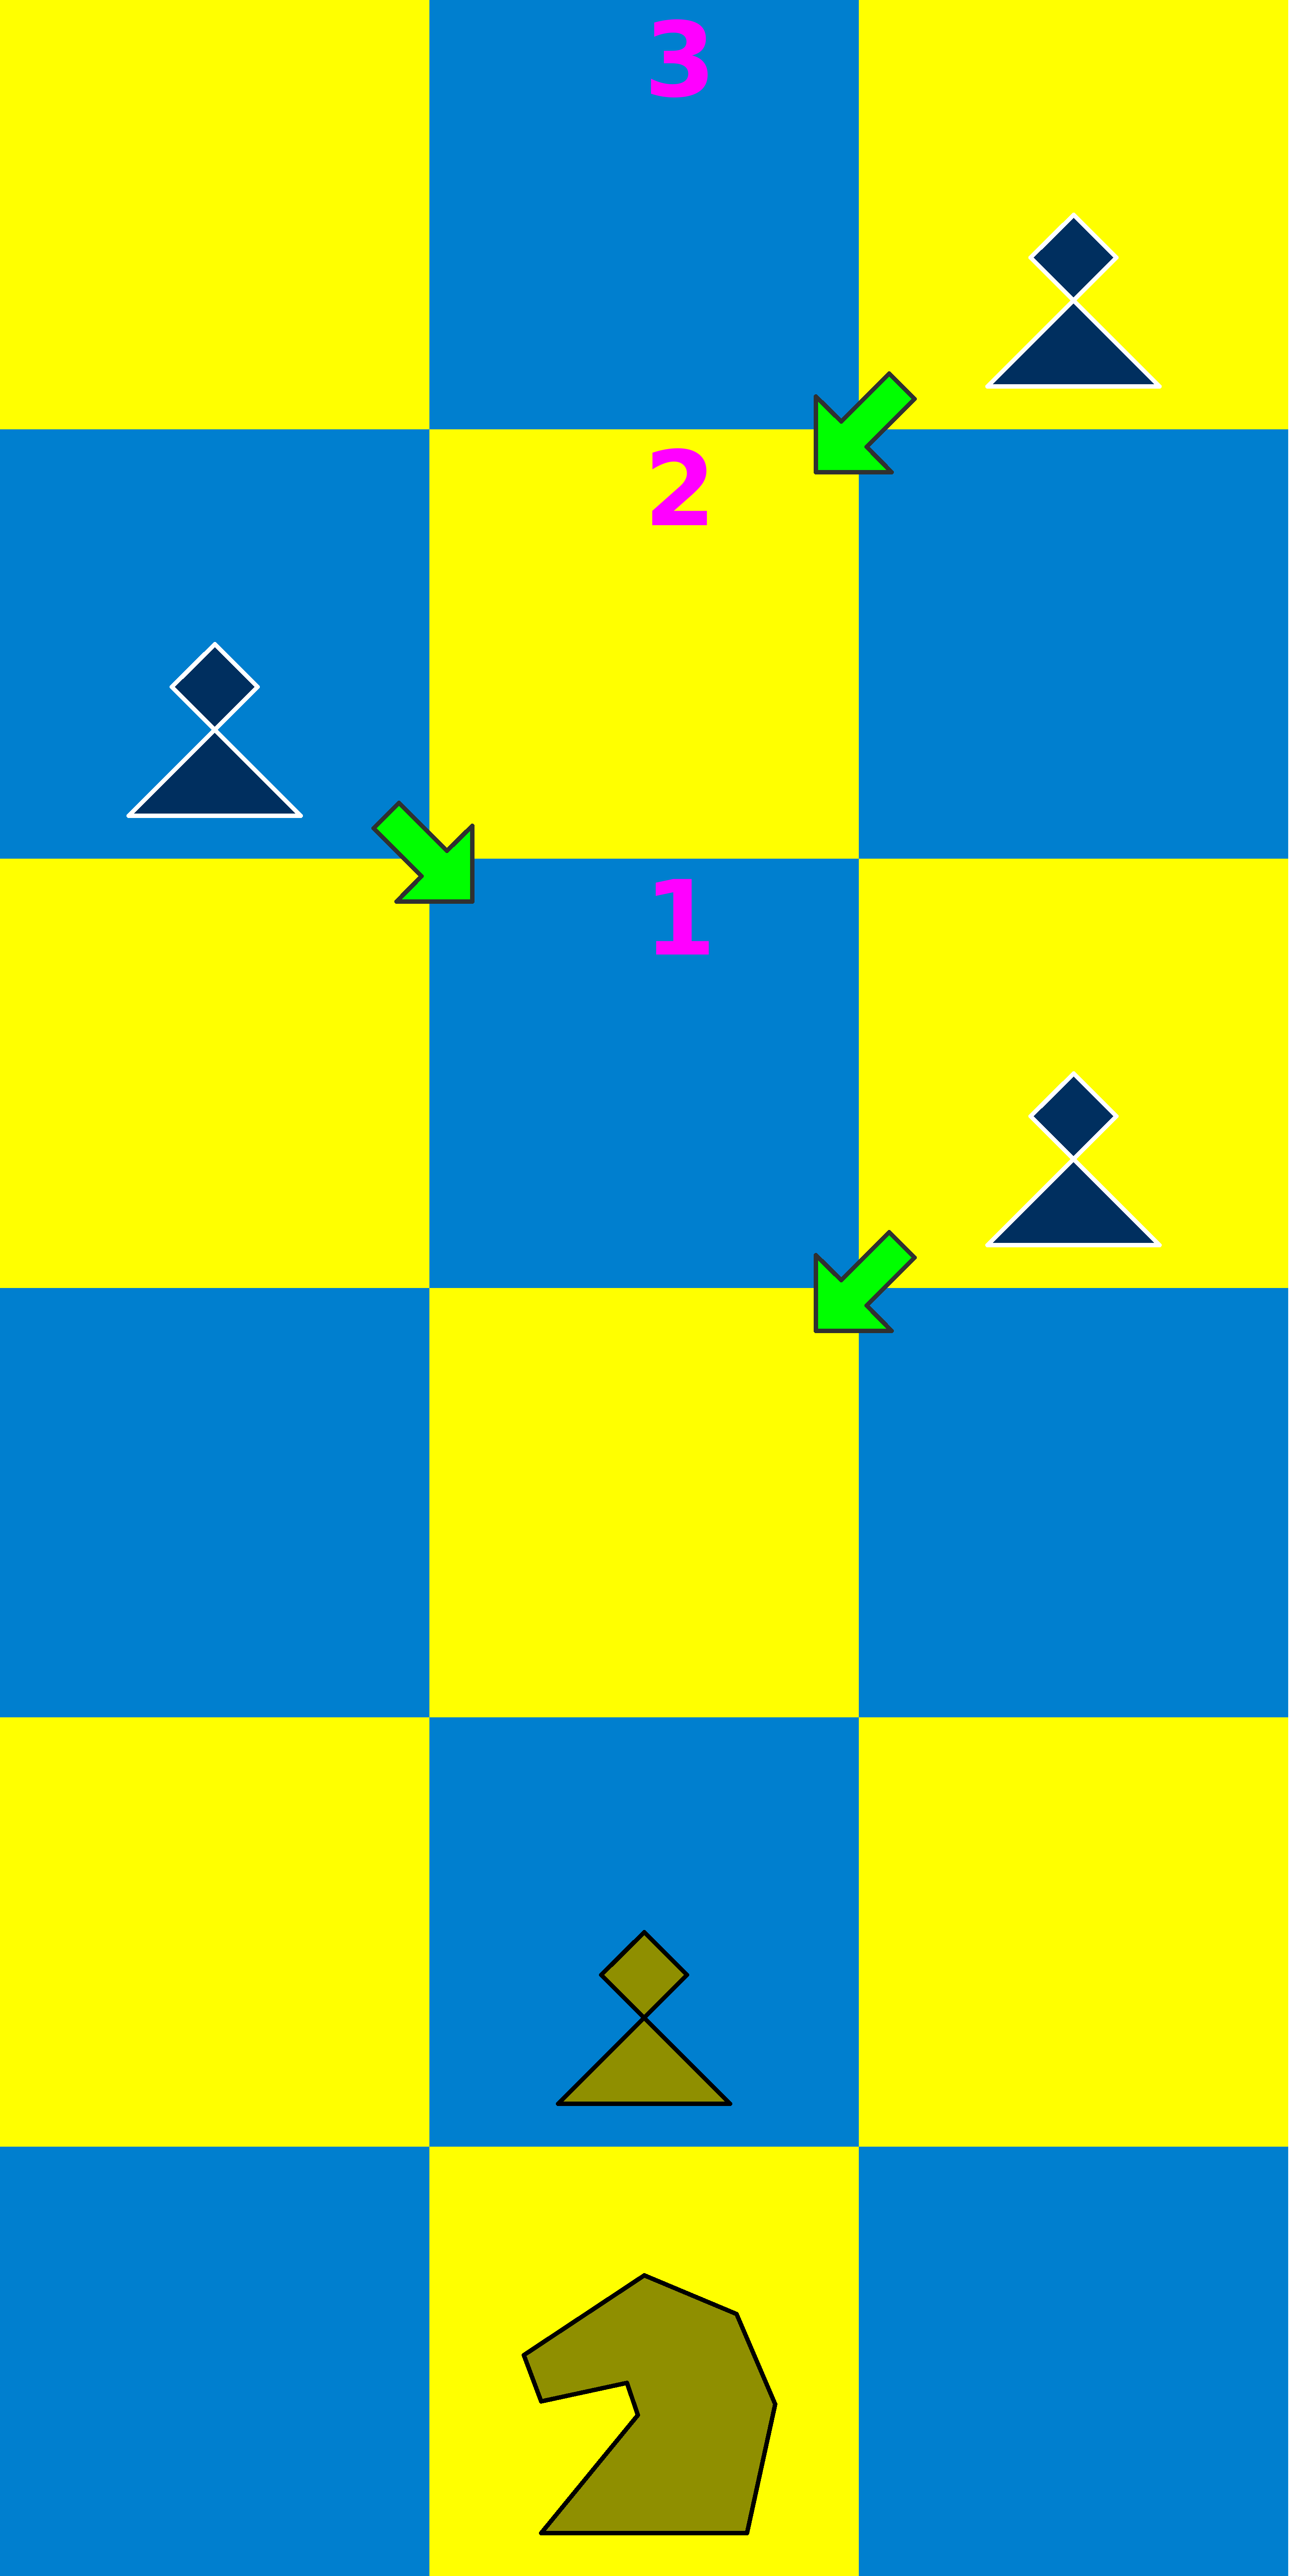
\includegraphics[width=0.25\textwidth, keepaspectratio=true]{en_passants/06_mayan_ascendancy_en_passant.png}
\caption{En passant}
\label{fig:06_mayan_ascendancy_en_passant}
\end{wrapfigure}
Rush and en passant are identical to those in Classic Chess, only difference
is that Pawn can now move longer on initial turn, up to 4 fields in this
variant.

\clearpage % ..........................................................

\section*{Castling}
\addcontentsline{toc}{section}{Castling}

Castling is essentially the same as it is in Classical Chess, only real difference is that
King can move 2, 3 or 4 fields across. All other constraints from Classical Chess still
applies.

\noindent
\begin{figure}[!h]
% \begin{figure}[!t]

\includegraphics[width=1.0\textwidth, keepaspectratio=true]{castlings/06_mayan_ascendancy_castling.png}
\caption{Castling}
\label{fig:06_mayan_ascendancy_castling}
% \centering
\end{figure}

In example above, all valid King's castling moves are numbered. Regardless if King performs
long or short castling move, Rook would always end up on the opposite side of King on the
field immediately next to it, i.e. closer to center.

\noindent
\begin{figure}[!h]
% \begin{figure}[!t]

\includegraphics[width=1.0\textwidth, keepaspectratio=true]{castlings/long_left/06_mayan_ascendancy_castling_long_left.png}
\caption{Castling long left}
\label{fig:06_mayan_ascendancy_castling_long_left}
% \centering
\end{figure}

In this example King was castling long to the left. Initial King's position is marked with "K".
After castling is finished, left Rook ends up at field immediately on the right to the King.

\clearpage % ..........................................................

\section*{Initial setup}
\addcontentsline{toc}{section}{Initial setup}

Compared to initial setup of Croatian Ties, Pyramid is inserted between Pegasus and Knight
symmetrically, on both sides of chessboard. This can be seen in the image below:

\noindent
% \begin{figure}[t]
\begin{figure}[h]
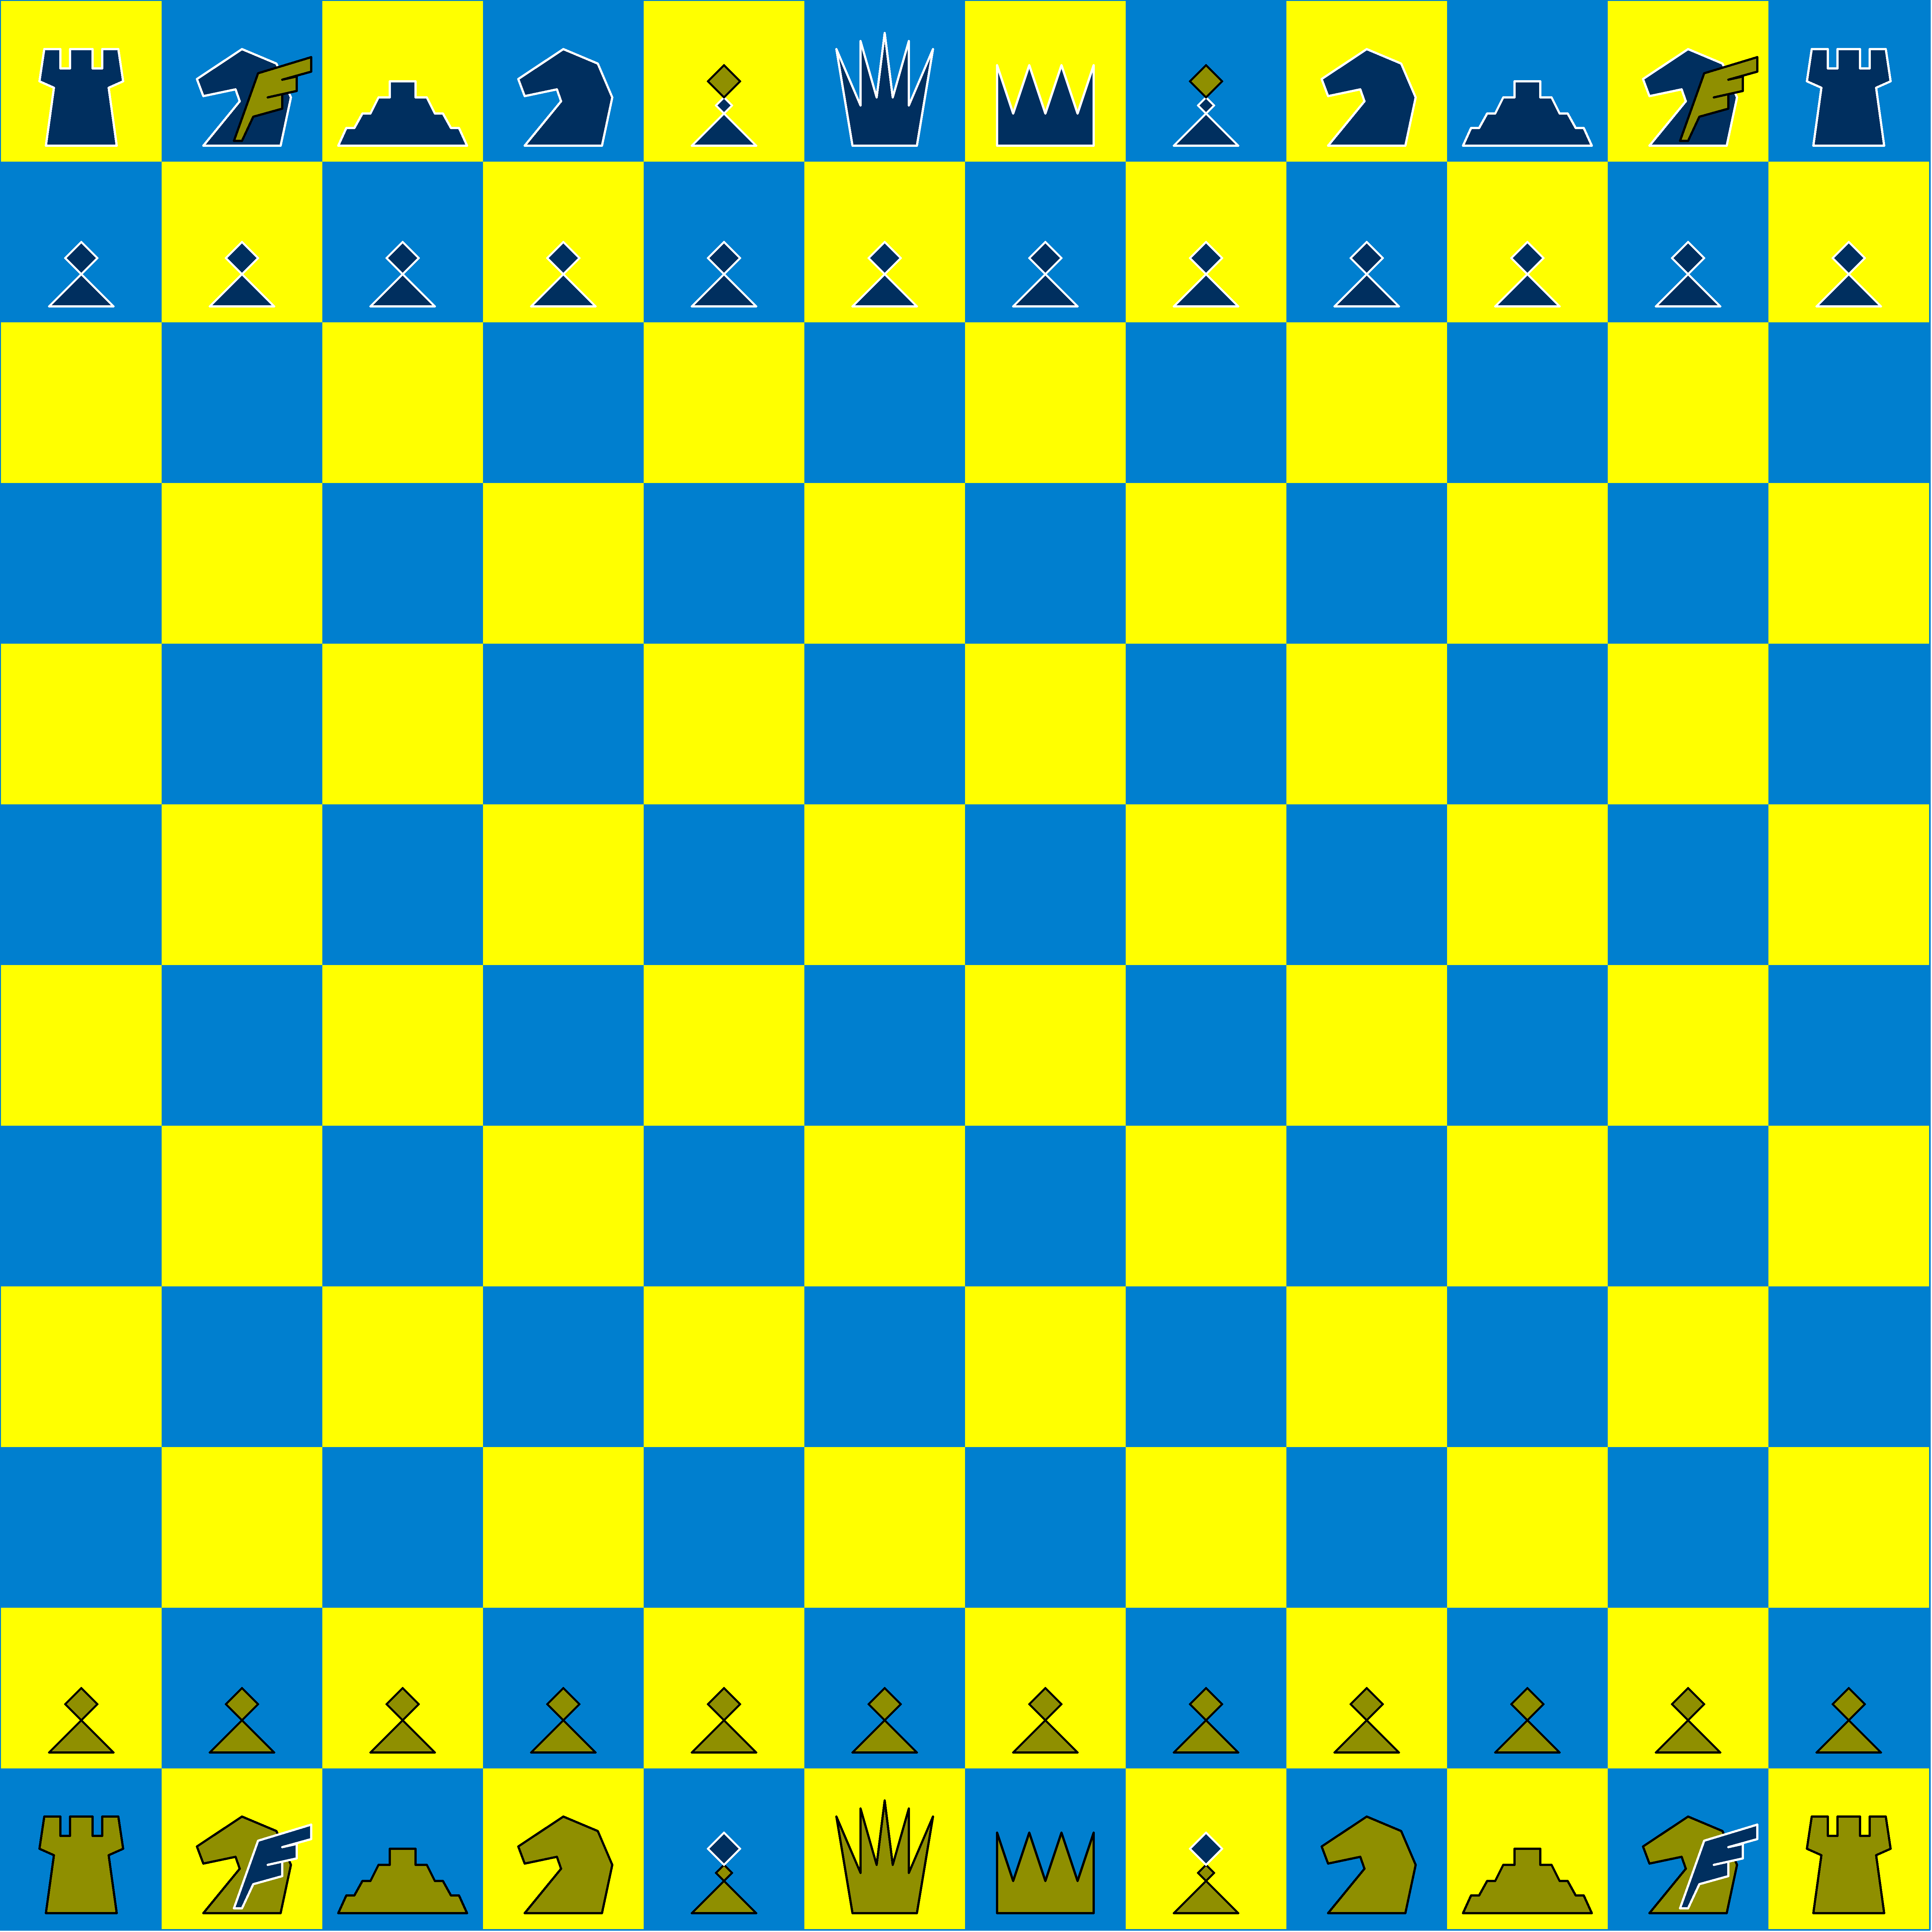
\includegraphics[width=1.0\textwidth, keepaspectratio=true]{boards/06_mayan_ascendancy.png}
\caption{Mayan Ascendancy board}
\label{fig:06_mayan_ascendancy}
% \centering
\end{figure}

\clearpage % ..........................................................
% -------------------------------------------- Mayan Ascendancy chapter

% -------------------------------------------- Mayan Ascendancy chapter

% Age of Aquarius chapter ---------------------------------------------

% Age of Aquarius chapter =============================================
\chapter*{Age of Aquarius}
\addcontentsline{toc}{chapter}{Age of Aquarius}

\begin{flushright}
\parbox{0.8\textwidth}{
\emph{The greatest difficulty with the world is not its ability to produce, but the unwillingness to share. \\
\hspace*{\fill}{\textperiodcentered \textperiodcentered \textperiodcentered \hspace*{0.2em} Roy L. Smith} } }
\end{flushright}

\noindent
Age of Aquarius is chess variant which is played on 14 x 14 board,
with light yellow and light green fields and light tan-gold and
dark green pieces. In algebraic notation, columns are enumerated
from 'a' to 'n', and rows are enumerated from '1' to '14'. A new
piece is introduced, Unicorn.

\clearpage % ..........................................................
% Unicorn *************************************************************

\section*{Unicorn}
\addcontentsline{toc}{section}{Unicorn}

\noindent
\begin{wrapfigure}[5]{l}{0.4\textwidth}
\centering
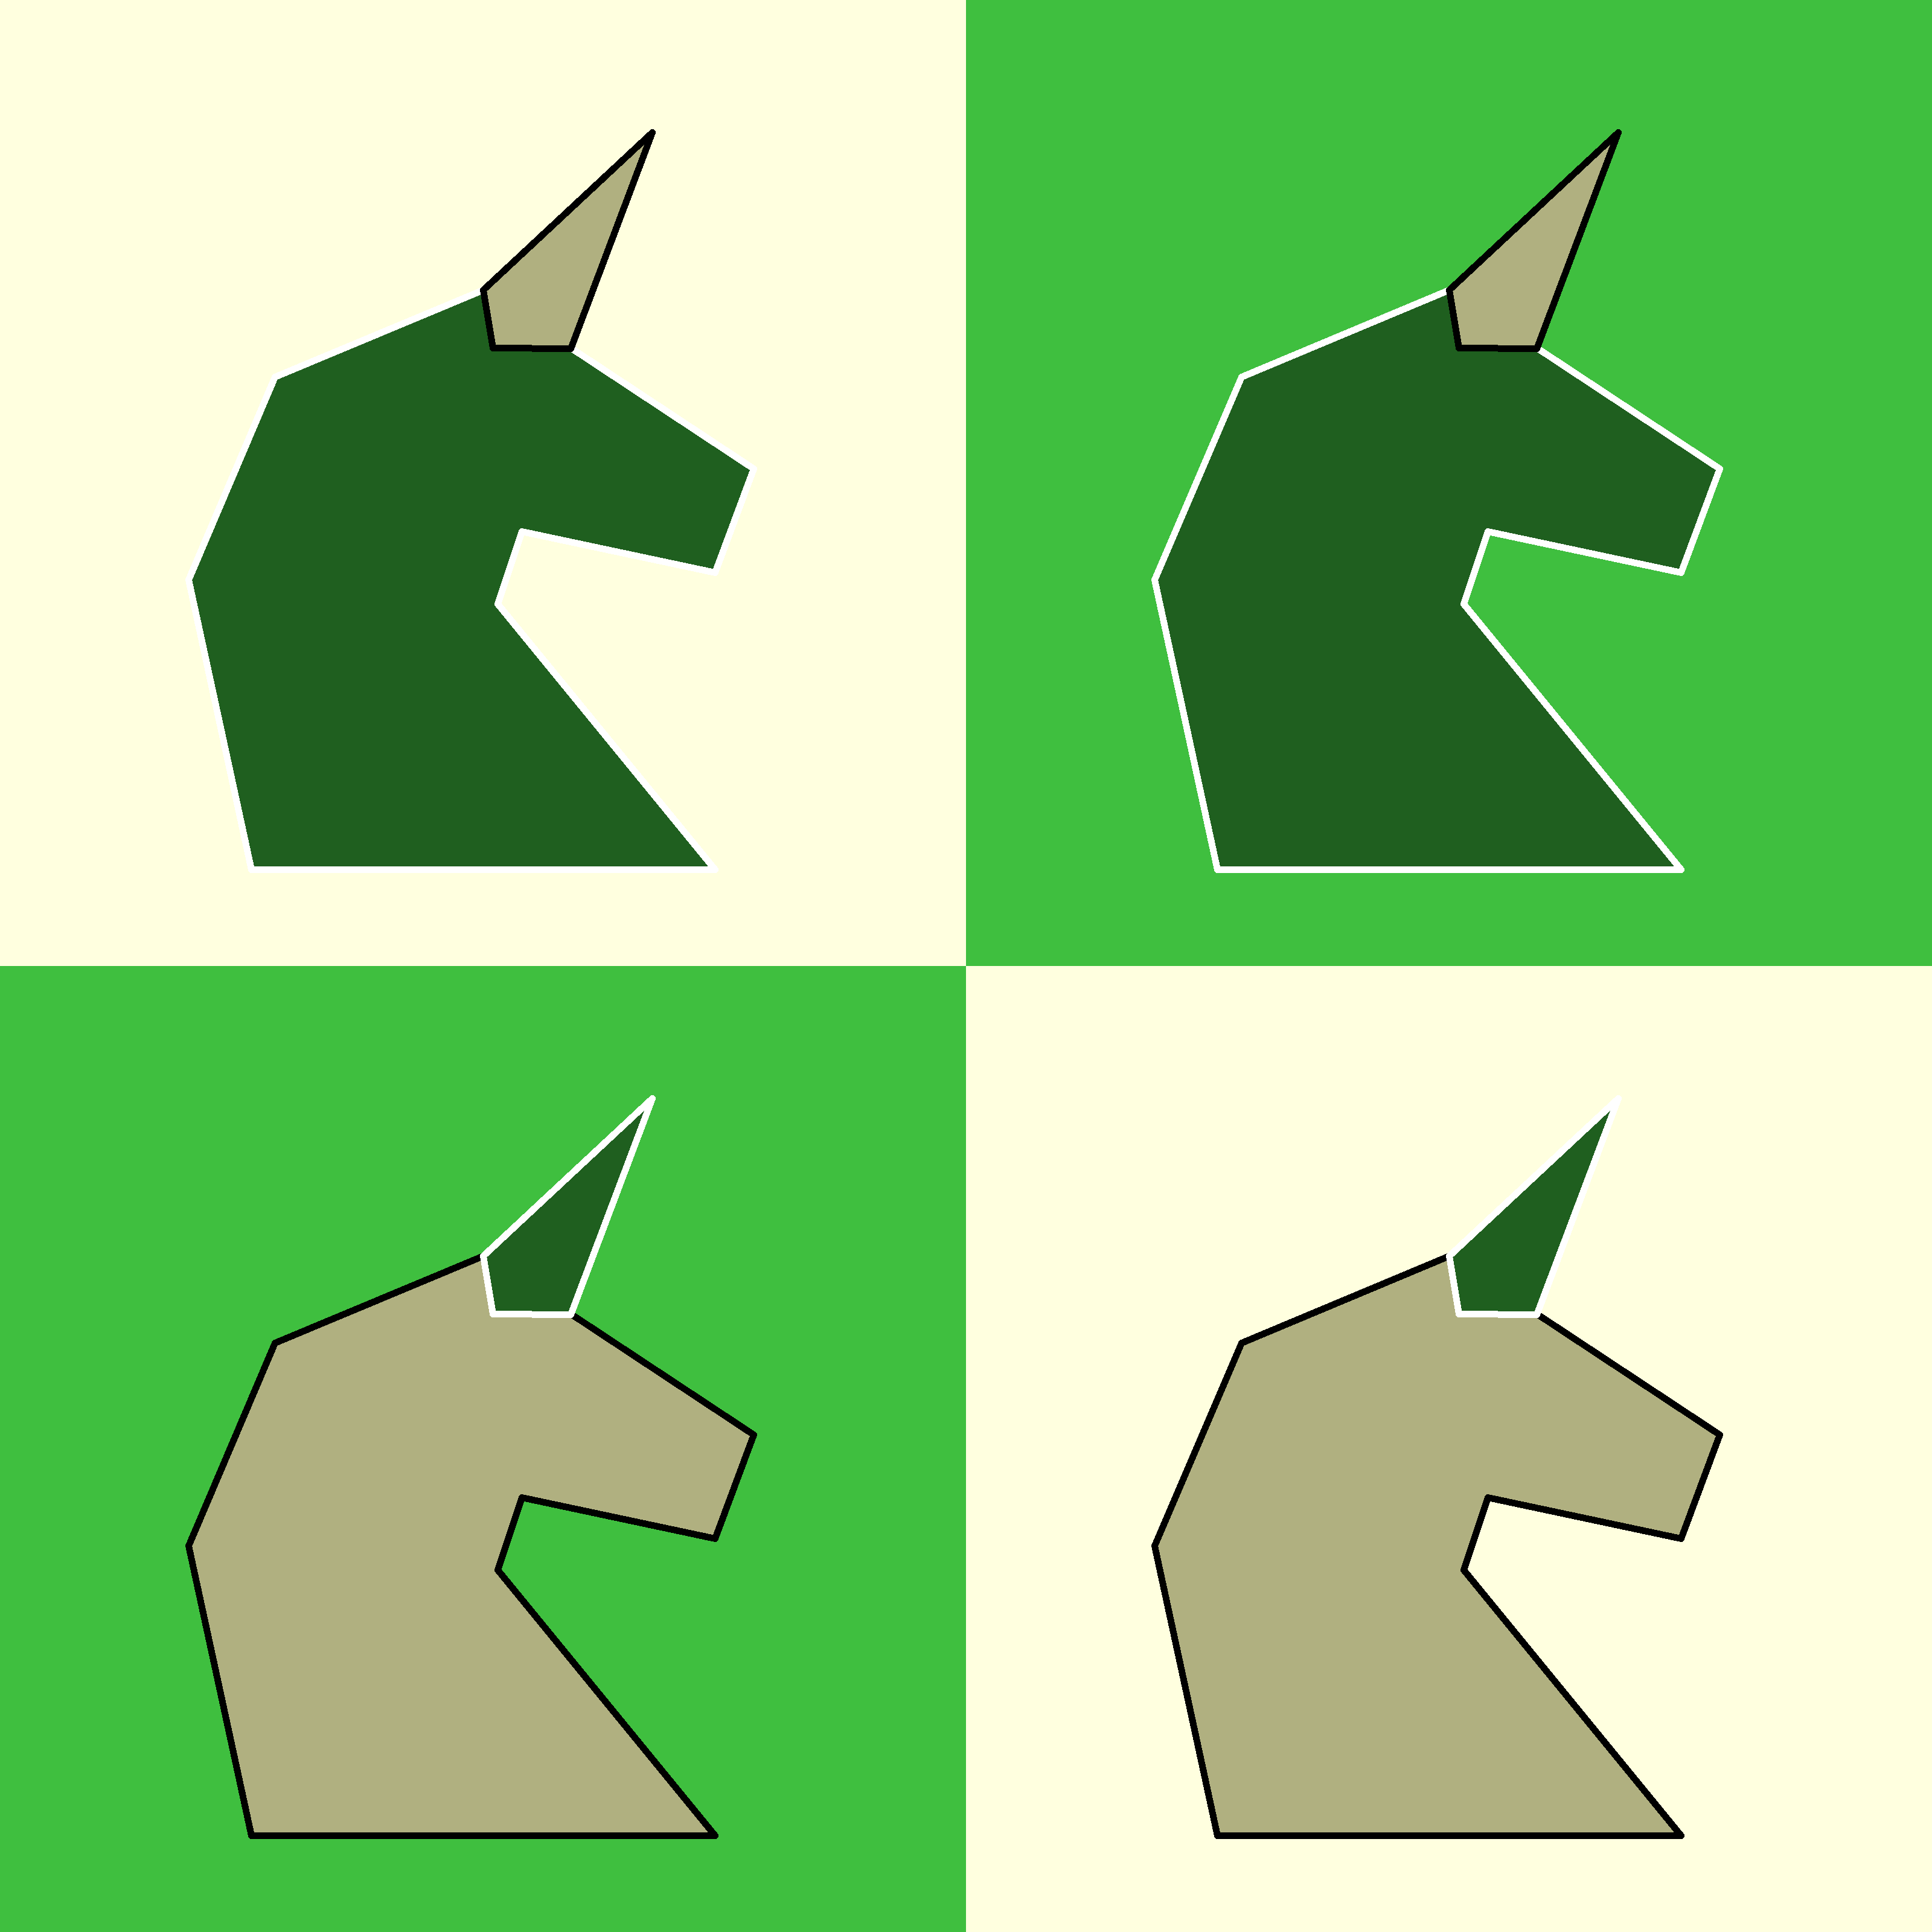
\includegraphics[width=0.4\textwidth, keepaspectratio=true]{pieces/09_unicorn.png}
\caption{Unicorn}
\label{fig:09_unicorn}
\end{wrapfigure}
Unicorn is a piece similar to Knight, only it can jump longer on
opposite color fields. Just as Knight, Unicorn is not obstructed
by any piece in its' surroundings.

\vspace{7\baselineskip}
\subsection*{Movement}
\addcontentsline{toc}{subsection}{Movement}

\noindent
\begin{wrapfigure}{l}{0.4\textwidth}
\centering
\includegraphics[width=0.4\textwidth, keepaspectratio=true]{examples/08_aoa/scn_aoa_01_unicorn_same_color.png}
\caption{Unicorn short jump}
\label{fig:scn_aoa_01_unicorn_same_color}
\end{wrapfigure}
On fields with the same color as Unicorn, it can move exactly the
same way Knight does.

\clearpage % ..........................................................

\noindent
\begin{figure}[!h]
% \begin{figure}[!t]
\includegraphics[width=1.0\textwidth, keepaspectratio=true]{examples/08_aoa/scn_aoa_02_unicorn_opposite_color.png}
\caption{Unicorn long jump}
\label{fig:scn_aoa_02_unicorn_opposite_color}
% \centering
\end{figure}

On fields in opposite color to Unicorn's, Unicorn can jump much longer.
Again, just as Knight, Unicorn is not hampered by surrouding pieces.
Only own pieces on marked (i.e. step) fields can prevent Unicorn to move,
opponent's pieces would be captured.

For comparison, Knight's step-fields are also numbered (grey).

% ************************************************************* Unicorn
\clearpage % ..........................................................
% Promotion ***********************************************************

\section*{Promotion}
\addcontentsline{toc}{section}{Promotion}
\label{sec:Age of Aquarius/Promotion}

In all variants prior to this one promotion was forced, Pawn had to be
promoted immediately upon reaching opposite end of chessboard (or when
reached by own Pyramid on opponent's side of board). Promotion otherwise
is identical to one in Classical Chess, which is described in details here: \\
\href{https://en.wikipedia.org/wiki/Promotion\_(chess)}{https://en.wikipedia.org/wiki/Promotion\_(chess)}.

In this variant promotion is not forced, Pawn does not have to be promoted
immediately. Moreover, Pawn can be actually promoted later in game, if it
hasn't moved between being tagged for promotion and actual promotion itself.
Delayed promotion is a complete move, it can contain only promotion of one
Pawn and nothing else.

\clearpage % ..........................................................

\noindent
% \begin{figure}[t]
\begin{figure}[h]
\includegraphics[width=1.0\textwidth, keepaspectratio=true]{examples/08_aoa/scn_aoa_03_delayed_promo_init.png}
\caption{Promotion start}
\label{fig:scn_aoa_03_delayed_promo_init}
% \centering
\end{figure}

Here, light player is about to tag Pawn 2 for promotion, using Pyramid
activated by Bishop. Note, Pawn 3 is not yet eligible for promotion, as it's
still on own side of chessboard.

\clearpage % ..........................................................

\noindent
% \begin{figure}[t]
\begin{figure}[h]
\includegraphics[width=1.0\textwidth, keepaspectratio=true]{examples/08_aoa/scn_aoa_04_delayed_promo_pawn_2_tagged.png}
\caption{Pawn 2 tagged for promotion}
\label{fig:scn_aoa_04_delayed_promo_pawn_2_tagged}
% \centering
\end{figure}

To speed things up, next images show dark player's response (grey arrow),
and light player's plan for next move (green arrow). Each depicted position
is after dark player's move, but before light player's move.

Here, dark Unicorn is attacking tagged Pawn 2. Pawn 2 is to move next.

\clearpage % ..........................................................

\noindent
% \begin{figure}[t]
\begin{figure}[h]
\includegraphics[width=1.0\textwidth, keepaspectratio=true]{examples/08_aoa/scn_aoa_05_delayed_promo_pawn_2_moved.png}
\caption{Pawn 1 about to get promotion}
\label{fig:scn_aoa_05_delayed_promo_pawn_2_moved}
% \centering
\end{figure}

Dark Unicorn closed in, attacking both Pawn 2 and Bishop. Since Pawn 2 moved
away from field P at which it was tagged for promotion, that opportunity has
been lost, and can't be recovered. Label P on a field just marks where Pawn 2
was tagged for promotion. Field P isn't special in any way, it won't make e.g.
Pawn 3 tagged for promotion when reached.

Light Pawn 1 is about to go next.

\clearpage % ..........................................................

\noindent
% \begin{figure}[t]
\begin{figure}[h]
\includegraphics[width=1.0\textwidth, keepaspectratio=true]{examples/08_aoa/scn_aoa_06_delayed_promo_pawn_1_tagged.png}
\caption{Pawn 1 tagged for promotion}
\label{fig:scn_aoa_06_delayed_promo_pawn_1_tagged}
% \centering
\end{figure}

Light Pawn 1 is now tagged for promotion, and is to be promoted later.
Dark Unicorn closed in again, capturing light Bishop.

Light Pawn 2 is about to go next.

\clearpage % ..........................................................

\noindent
% \begin{figure}[t]
\begin{figure}[h]
\includegraphics[width=1.0\textwidth, keepaspectratio=true]{examples/08_aoa/scn_aoa_07_delayed_promo_pawn_1_promoted.png}
\caption{Pawn 1 promoted}
\label{fig:scn_aoa_07_delayed_promo_pawn_1_promoted}
% \centering
\end{figure}

Dark Unicorn captures light Pawn 2.

Light Pawn 1 is promoted to Queen.

\clearpage % ..........................................................
% Converting tagged Pawn ----------------------------------------------

\subsection*{Converting tagged Pawn}
\addcontentsline{toc}{subsection}{Converting tagged Pawn}

Converting opponent's Pawns tagged for promotion in own first row grants them
ability to be rushed, and subjects them to opponent's en passant move.

\noindent
% \begin{figure}[t]
\begin{figure}[h]
\includegraphics[width=1.0\textwidth, keepaspectratio=true]{examples/08_aoa/scn_aoa_11_tagged_pawn_conv_init.png}
\caption{Opponent's Pawn to be tagged}
\label{fig:scn_aoa_11_tagged_pawn_conv_init}
% \centering
\end{figure}

Here, dark Pawn is about to be promoted/tagged for promotion, as it approaches
it's last row.

\clearpage % ..........................................................

\noindent
% \begin{figure}[t]
\begin{figure}[h]
\includegraphics[width=1.0\textwidth, keepaspectratio=true]{examples/08_aoa/scn_aoa_12_tagged_pawn_conv_tagged.png}
\caption{Opponent's Pawn tagged for promotion}
\label{fig:scn_aoa_12_tagged_pawn_conv_tagged}
% \centering
\end{figure}

Now that dark Pawn is tagged for promotion, it get's converted by Pyramid,
which was activated by Bishop.

Normally, Pawn gets promoted right away, because it saves move and makes better
figure available immediately. In this case, however, it would allow opponent
(light player) to convert e.g., Queen. By just tagging a Pawn, it makes it a
latent threat, without overwhelming gains.

\clearpage % ..........................................................

\noindent
% \begin{figure}[t]
\begin{figure}[h]
\includegraphics[width=1.0\textwidth, keepaspectratio=true]{examples/08_aoa/scn_aoa_13_tagged_pawn_converted.png}
\caption{Rushing converted Pawn}
\label{fig:scn_aoa_13_tagged_pawn_converted}
% \centering
\end{figure}

Converted Pawn now can be rushed, up to the row reachable by ordinary Pawn 1.
As with ordinary rush, it can only be performed from Pawn's initial position.

Generaly, all Pawns (own or converted) can be rushed up to the (and including)
furthest own row of chessboard, i.e. after rush they still have to reside on
own side of the board. Pawns can only be rushed from
\hyperref[sec:Terms/Pawn row]{Pawn} and \hyperref[sec:Terms/Figure row]{figure} rows.

% ---------------------------------------------- Converting tagged Pawn
% *********************************************************** Promotion
\clearpage % ..........................................................

\section*{En passant}
\addcontentsline{toc}{section}{En passant}

\noindent
\begin{wrapfigure}{l}{0.4\textwidth}
\centering
\includegraphics[width=0.214285714286\textwidth, keepaspectratio=true]{en_passants/08_age_of_aquarius_en_passant.png}
\caption{En passant}
\label{fig:08_age_of_aquarius_en_passant}
\end{wrapfigure}
Rush and en passant are identical to those in Classic Chess, only difference
is that Pawn can now move longer on initial turn, up to 5 fields in this
variant.

\clearpage % ..........................................................

\section*{Castling}
\addcontentsline{toc}{section}{Castling}

Castling is the same as in Classical Chess, only difference is that King can move 2, 3, 4 or 5 fields across.
All other constraints from Classical Chess still applies.

\noindent
\begin{figure}[!h]
% \begin{figure}[!t]
\includegraphics[width=1.0\textwidth, keepaspectratio=true]{castlings/08_aoa/age_of_aquarius_castling.png}
\caption{Castling}
\label{fig:age_of_aquarius_castling}
% \centering
\end{figure}

In example above, all valid King's castling moves are numbered.

\noindent
\begin{figure}[!h]
% \begin{figure}[!t]
\includegraphics[width=1.0\textwidth, keepaspectratio=true]{castlings/08_aoa/age_of_aquarius_castling_left_04.png}
\caption{Castling long left}
\label{fig:age_of_aquarius_castling_left_04}
% \centering
\end{figure}

In this example King was castling long to the left. Initial King's position is marked with "K".
After castling is finished, left Rook ends up on the field immediately right to the King.

\clearpage % ..........................................................

\section*{Initial setup}
\addcontentsline{toc}{section}{Initial setup}

Compared to initial setup of Mayan Ascendancy, Unicorn is inserted between Pyramid and Knight
symmetrically, on both sides of chessboard. This can be seen in the image below:

\noindent
% \begin{figure}[t]
\begin{figure}[h]
\includegraphics[width=1.0\textwidth, keepaspectratio=true]{boards/08_age_of_aquarius.png}
\caption{Age of Aquarius board}
\label{fig:08_age_of_aquarius}
% \centering
\end{figure}

\clearpage % ..........................................................
% ============================================= Age of Aquarius chapter

% --------------------------------------------- Age of Aquarius chapter

% Miranda's veil chapter ----------------------------------------------

% Copyright (c) 2015 - 2020 Mario Mlačak, mmlacak@gmail.com
% Licensed and published as Public Domain work.

% Miranda's veil chapter ==============================================
\chapter*{Miranda's veil}
\addcontentsline{toc}{chapter}{Miranda's veil}

\begin{flushright}
\parbox{0.8\textwidth}{
\emph{Under all that we think, lives all we believe, like the ultimate veil of our spirits. \\
\hspace*{\fill}{\textperiodcentered \textperiodcentered \textperiodcentered \hspace*{0.2em} Antonio Machado} } }
\end{flushright}

\noindent
Miranda's veil is chess variant which is played on 16 x 16 board, with
white and dark violet fields and light magenta and indigo pieces. In
algebraic notation, columns are enumerated from 'a' to 'p', and rows
are enumerated from '1' to '16'. A new piece is introduced, Wave.

\clearpage % ..........................................................
% Wave ****************************************************************

\section*{Wave}
\addcontentsline{toc}{section}{Wave}

\vspace*{-1.0ex}
\noindent
\begin{wrapfigure}[12]{l}{0.4\textwidth}
\centering
\includegraphics[width=0.4\textwidth, keepaspectratio=true]{pieces/10_wave.png}
\caption{Wave}
\label{fig:10_wave}
\end{wrapfigure}
Wave is passive piece, it has to be activated before it can move. Activation
is done in the same way as with Pyramid. Own piece has to capture field at
which Wave is located before Wave can move.

Wave can be activated even if activating piece has no momentum. Wave does not use
received momentum for moving, and isn't limited by it. Wave can move even if it
has no momentum. Wave can move past (pass "through") any piece, as if it isn't there.

After activation Wave moves like activating piece, over piece's step- or capture-
fields, depending where it was activated. Wave can make multiple steps, in the
same way activating piece does, even if activating piece can make only one. Note,
Wave can choose direction on the first 1 or 2 step(s), which cannot be changed
later. Wave can step outside of a chessboard, and only has to end its ply on a
board. For details see
\hyperref[sec:Appendix/Movement of Wave]{Movement of Wave}.

Wave cannot capture any piece. Thus, Wave cannot check nor checkmate opponent's
King.

Wave can activate any own piece, except King, if it has momentum. Wave can
also activate other Wave, own or opponent's, even if it has no momentum. In
all cases, Wave transfers all received momentum to activated piece.

In algebraic notation symbol for Wave is 'W'.

\clearpage % ..........................................................
% Activation ----------------------------------------------------------

\subsection*{Activation}
\addcontentsline{toc}{subsection}{Activation}

\vspace*{-2.0ex}
\noindent
% \begin{figure}[t]
\begin{figure}[h]
\includegraphics[width=1.0\textwidth, keepaspectratio=true]{examples/10_mv/scn_mv_01_move_wave_init.png}
\caption{Wave activation}
\label{fig:scn_mv_01_move_wave_init}
% \centering
\end{figure}

Above, after activation Wave could move the same way Knight does, over multiple
step-fields. So, in this case Wave would move as Pegasus does. Once Wave starts
moving in a chosen direction, it cannot be changed. Wave does not spend received
momentum while moving, and would transfer it entirely to any piece it activates.

\clearpage % ..........................................................

\noindent
% \begin{figure}[t]
\begin{figure}[h]
\includegraphics[width=1.0\textwidth, keepaspectratio=true]{examples/10_mv/scn_mv_02_move_wave_activated.png}
\caption{Wave activated}
\label{fig:scn_mv_02_move_wave_activated}
% \centering
\end{figure}

Wave can move unhindered by any piece, even on step-fields (green arrows). Wave
can also activate pieces (blue arrows) obscured by others, for instance light
Pyramid which is out of reach for regular Pegasus. Wave cannot activate Kings nor
opponent's pieces (red arrows), except dark Wave. \\
Again, Wave cannot change direction of movement after first step. For instance,
upon reaching step-field 5, it cannot change direction to 5c, or any other
greyed-out direction.

\clearpage % ..........................................................

\noindent
% \begin{figure}[t]
\begin{figure}[h]
\includegraphics[width=1.0\textwidth, keepaspectratio=true]{examples/10_mv/scn_mv_03_move_wave_finished.png}
\caption{Wave finished}
\label{fig:scn_mv_03_move_wave_finished}
% \centering
\end{figure}

Greyed-out arrows show steps light Wave have taken in its ply. Activated Bishop
now continues the move according to own rules of movement, i.e. diagonally. Note
that it's restricted by momentum received, and thus can make only one step, i.e.
can move for only one field.

\clearpage % ..........................................................

\subsubsection*{Cascading Waves}
\addcontentsline{toc}{subsubsection}{Cascading Waves}

\vspace*{-3.0ex}
\noindent
% \begin{figure}[t]
\begin{figure}[h]
\includegraphics[width=1.0\textwidth, keepaspectratio=true]{examples/10_mv/scn_mv_04_wave_cascading_init.png}
\caption{Cascade start}
\label{fig:scn_mv_04_wave_cascading_init}
% \centering
\end{figure}

Activated Wave inherits way of movement from activating piece,
\hyperref[sec:Appendix/Movement of Wave]{rules of inheritance are simple, with few exceptions}.
When activated by other Wave, movement of an activated Wave is exactly the same as
activating Wave.

Here, Wave B moves like a Bishop, because activating Wave A moved like a Bishop,
since it was activated by one.

\clearpage % ..........................................................

\vspace*{-5.0ex}
\noindent
% \begin{figure}[t]
\begin{figure}[h]
\includegraphics[width=1.0\textwidth, keepaspectratio=true]{examples/10_mv/scn_mv_05_wave_cascading_steps.png}
\caption{Active piece cascaded}
\label{fig:scn_mv_05_wave_cascading_steps}
% \centering
\end{figure}

When piece activated in a cascade is not a Wave, it has its own rules of movement, and
Waves activated afterwards inherit them from that activating piece.

Here, all Waves activated after Knight moves like multi-step Knight (i.e. Pegasus),
since Waves are not restricted to only one step, even if activating piece is.

\clearpage % ..........................................................

\vspace*{-5.0ex}
\noindent
% \begin{figure}[t]
\begin{figure}[h]
\includegraphics[width=1.0\textwidth, keepaspectratio=true]{examples/10_mv/scn_mv_06_wave_cascading_end.png}
\caption{Cascade end}
\label{fig:scn_mv_06_wave_cascading_end}
% \centering
\end{figure}

First piece in a cascade gathers momentum over step-fields travelled. All pieces
transfer any remaining momentum to the next piece in a cascade. Waves do not spend
received momentum for movement, but all the other pieces do.

Here, numbers in lower, left corner are received momentum. Bishop gathered 3 momentum,
1 has been spent by Knight, and so activated Pawn can be rushed for only 2 fields.

\clearpage % ..........................................................

\subsubsection*{Cascading opponent}
\addcontentsline{toc}{subsubsection}{Cascading opponent}

. . .

\clearpage % ..........................................................

\subsubsection*{No momentum}
\addcontentsline{toc}{subsubsection}{No momentum}

\vspace*{-3.0ex}
\noindent
% \begin{figure}[t]
\begin{figure}[h]
\includegraphics[width=1.0\textwidth, keepaspectratio=true]{examples/10_mv/scn_mv_07_wave_no_momentum_no_activating.png}
\caption{No momentum}
\label{fig:scn_mv_07_wave_no_momentum_no_activating}
% \centering
\end{figure}

Wave can be activated with no momentum, if so it can activate only other Waves, but
cannot activate ordinary (non-Wave) pieces. Here, one momentum originating from Bishop
has been already spent by Knight, so Wave B is activated with no momentum, and so it
cannot activate Pawn. Wave B can pass-by Pawn, and activate dark Wave, also with no
momentum.

\clearpage % ..........................................................

\subsubsection*{Piece blocked}
\addcontentsline{toc}{subsubsection}{Piece blocked}

\vspace*{-3.0ex}
\noindent
% \begin{figure}[t]
\begin{figure}[h]
\includegraphics[width=1.0\textwidth, keepaspectratio=true]{examples/10_mv/scn_mv_08_wave_no_activating_blocked_piece.png}
\caption{Piece blocked}
\label{fig:scn_mv_08_wave_no_activating_blocked_piece}
% \centering
\end{figure}

Wave cannot activate blocked pieces, even if it has momentum. Here, Pawn is blocked
from moving forward by own Bishop, and there are no opponent's pieces on its'
diagonal capture-fields. So, Wave cannot activate Pawn, even though it has one
momentum received from Knight.

\clearpage % ..........................................................

\subsubsection*{Wave blocked}
\addcontentsline{toc}{subsubsection}{Wave blocked}

\vspace*{-3.0ex}
\noindent
% \begin{figure}[t]
\begin{figure}[h]
\includegraphics[width=1.0\textwidth, keepaspectratio=true]{examples/10_mv/scn_mv_09_wave_blocked_init.png}
\caption{Activating Wave}
\label{fig:scn_mv_09_wave_blocked_init}
% \centering
\end{figure}

Wave cannot activate opponent's pieces, except for Waves. Activated Wave which movement
is completely blocked is oblationed, i.e. is removed from chessboard as if captured by
opponent.

Here, dark Wave B is about to be activated with one momentum.

\clearpage % ..........................................................

\vspace*{-5.0ex}
\noindent
% \begin{figure}[t]
\begin{figure}[h]
\includegraphics[width=1.0\textwidth, keepaspectratio=true]{examples/10_mv/scn_mv_10_wave_blocked_end.png}
\caption{Activated Wave blocked}
\label{fig:scn_mv_10_wave_blocked_end}
% \centering
\end{figure}

Here, dark Wave B is activated without committing its movement yet (it's "in-the-air").
All accessible step-fields are blocked by opponent's light pieces, which cannot be
activated by dark Wave, even though it has one momentum.
Note, Wave (just like any other piece) has to move away from its starting position,
it cannot stay and re-activate piece that has activated it (here, light Wave 2).
Thus, dark Wave B is oblationed, i.e. removed from chessboard.

% ---------------------------------------------------------- Activation
\clearpage % ..........................................................
% Cascading Waves -----------------------------------------------------

\subsection*{Cascading Waves}
\addcontentsline{toc}{subsection}{Cascading Waves}

\noindent
\begin{wrapfigure}[13]{l}{0.5625\textwidth}
\centering
\includegraphics[width=0.5625\textwidth, keepaspectratio=true]{examples/10_mv/scn_mv_11_cascading_rook.png}
\caption{Rook starting cascade}
\label{fig:scn_mv_11_cascading_rook}
\end{wrapfigure}
Cascading Waves refers to a move in which two or more Waves have been displaced.
For example, Wave can activate another Wave. Wave can also activate active
piece (or Pyramid), which can then activate another Wave.

On the left, Rook is about to activate Wave 1, giving it momentum of 4.

\vspace*{0.05\textheight}
\noindent
\begin{wrapfigure}[12]{r}{0.5625\textwidth}
\centering
\includegraphics[width=0.5625\textwidth, keepaspectratio=true]{examples/10_mv/scn_mv_12_cascading_wave_1.png}
\caption{Wave 1 cascading}
\label{fig:scn_mv_12_cascading_wave_1}
\end{wrapfigure}
Activated Wave 1 inherits rules of movement from activating piece, and so now
moves as Rook would. It's not obstructed with any piece in its way, nor it's
limited by received momentum, i.e. it can move further than just 4 fields away.
Wave 1 can also activate Wave 2.

\clearpage % ..........................................................

\noindent
\begin{wrapfigure}[13]{l}{0.5625\textwidth}
\centering
\includegraphics[width=0.5625\textwidth, keepaspectratio=true]{examples/10_mv/scn_mv_13_cascading_wave_2.png}
\caption{Wave 2 cascading}
\label{fig:scn_mv_13_cascading_wave_2}
\end{wrapfigure}
Activated Wave 2 inherits rules of movement from activating piece (in this
case Wave 1), and so too moves as Rook would. Wave 2 also received momentum
of 4. Again, it's not obstructed by any piece, nor it's limited by received
momentum. Wave 2 can also activate either Queen or Rook.

\vspace*{0.075\textheight}
\noindent
\begin{wrapfigure}[15]{r}{0.5625\textwidth}
\centering
\includegraphics[width=0.5625\textwidth, keepaspectratio=true]{examples/10_mv/scn_mv_14_cascading_rook_2nd_time.png}
\caption{Rook, 2nd cascading}
\label{fig:scn_mv_14_cascading_rook_2nd_time}
\end{wrapfigure}
Rook is now activated, but it is limited by momentum received, i.e. it can
move at most 4 fields away. Naturaly, Rook is obstructed by surrounding pieces,
i.e. it can't move past Wave 1. Rook can activate Wave 1.

Note, piece for each activation in a cascade can choose any legal direction of
movement for that ply, independent of what was chosen for previous plies.

\clearpage % ..........................................................

\noindent
\begin{wrapfigure}[10]{l}{0.5625\textwidth}
\centering
\includegraphics[width=0.5625\textwidth, keepaspectratio=true]{examples/10_mv/scn_mv_15_cascading_wave_1_2nd_time.png}
\caption{Wave 1, 2nd cascading}
\label{fig:scn_mv_15_cascading_wave_1_2nd_time}
\end{wrapfigure}
Activated Wave 1 received momentum of 2 and rules of movement from Rook. Again,
Wave 1 is not obstructed by any piece, nor it is limited by received momentum.
Wave 1 can also activate either Queen or Wave 2.

\vspace*{0.155\textheight}
\noindent
\begin{wrapfigure}[10]{r}{0.5625\textwidth}
\centering
\includegraphics[width=0.5625\textwidth, keepaspectratio=true]{examples/10_mv/scn_mv_16_cascading_queen.png}
\caption{Queen cascading}
\label{fig:scn_mv_16_cascading_queen}
\end{wrapfigure}
Activated Queen received momentum of 2, it can move at most 2 fields away.
Queen can also activate Wave 2, giving it momentum of 0.

\clearpage % ..........................................................

\noindent
\begin{wrapfigure}[7]{l}{0.5625\textwidth}
\centering
\includegraphics[width=0.5625\textwidth, keepaspectratio=true]{examples/10_mv/scn_mv_17_cascading_wave_2_2nd_time.png}
\caption{Wave 2, 2nd cascading}
\label{fig:scn_mv_17_cascading_wave_2_2nd_time}
\end{wrapfigure}
Activated Wave 2 received rules of movement from Queen, and 0 momentum.
Note, since Wave 2 has no momentum it can't activate Rook, only Wave 1.

\vspace*{0.245\textheight}
\noindent
\begin{wrapfigure}[9]{r}{0.5625\textwidth}
\centering
\includegraphics[width=0.5625\textwidth, keepaspectratio=true]{examples/10_mv/scn_mv_18_cascading_wave_1_3rd_time.png}
\caption{Wave 1, 3rd cascading}
\label{fig:scn_mv_18_cascading_wave_1_3rd_time}
\end{wrapfigure}
Activated Wave 1 inherits rules of movement from activating piece (Wave 2),
meaning Wave 1 too now moves as Queen would. Due to no momentum, Wave 1 can't
activate neither Queen nor Rook.

\clearpage % ..........................................................

\noindent
\begin{wrapfigure}[3]{l}{0.5625\textwidth}
\centering
\includegraphics[width=0.5625\textwidth, keepaspectratio=true]{examples/10_mv/scn_mv_19_cascading_end.png}
\caption{Wave 1, end cascading}
\label{fig:scn_mv_19_cascading_end}
\end{wrapfigure}
Wave 1 end this rather long cascade by settling past Rook.

\vspace*{0.345\textheight}
In a cascade, Wave is not limited by received momentum, nor it's obstructed by
other pieces on board. Wave inherts rules of movement from activating piece,
and can make multiple steps, even if activating piece can make only one.
For details see \hyperref[sec:Appendix/Movement of Wave]{Movement of Wave}
in Definitions. All other pieces moves according to their own rules, and are
restricted by momentum received.

During cascade, after each ply activation takes place according to current
positions of pieces on the board, just as it would at the beginning of the move.
For each activation in a cascade, all pieces can choose any legal direction
independently of previous choices.

This makes it possible, in the same cascade, to activate piece which started it,
Rook in this example. Such cascade is said to feature push-pull activation.
It's also possible to reactivate other (non-initiating) pieces in the same
cascade, e.g. here Wave 1 was reactivated 3 times.

% ----------------------------------------------------- Cascading Waves
\clearpage % ..........................................................
% Cascading opponent --------------------------------------------------

\subsection*{Cascading opponent}
\addcontentsline{toc}{subsection}{Cascading opponent}

\noindent
\begin{wrapfigure}[10]{l}{0.5625\textwidth}
\centering
\includegraphics[width=0.5625\textwidth, keepaspectratio=true]{examples/10_mv/scn_mv_20_casc_oppo_light_queen.png}
\caption{Light Queen starting cascade}
\label{fig:scn_mv_20_casc_oppo_light_queen}
\end{wrapfigure}
Cascading opponent refers to a move in which opponent's Wave has been displaced,
potentially other opponent's pieces.

On the left, light Queen is about to activate light Wave, giving it momentum of 3.

\vspace*{0.155\textheight}
\noindent
\begin{wrapfigure}[5]{r}{0.5625\textwidth}
\centering
\includegraphics[width=0.5625\textwidth, keepaspectratio=true]{examples/10_mv/scn_mv_21_casc_oppo_light_wave.png}
\caption{Light Wave}
\label{fig:scn_mv_21_casc_oppo_light_wave}
\end{wrapfigure}
Activated light Wave can activate dark Wave, but can't interact with dark Queen in
any way.

\clearpage % ..........................................................

\noindent
\begin{wrapfigure}[5]{l}{0.5625\textwidth} % 5 bch % 4 lmc
\centering
\includegraphics[width=0.5625\textwidth, keepaspectratio=true]{examples/10_mv/scn_mv_22_casc_oppo_dark_wave.png}
\caption{Dark Wave}
\label{fig:scn_mv_22_casc_oppo_dark_wave}
\end{wrapfigure}
Activated dark Wave now can activate dark Queen, but cannot interact with light Queen
in any way.

\vspace*{0.315\textheight}
\noindent
\begin{wrapfigure}[13]{r}{0.5625\textwidth} % 13 bch % 12 lmc
\centering
\includegraphics[width=0.5625\textwidth, keepaspectratio=true]{examples/10_mv/scn_mv_23_casc_oppo_dark_queen.png}
\caption{Dark Queen}
\label{fig:scn_mv_23_casc_oppo_dark_queen}
\end{wrapfigure}
Activated dark Queen is limited to momentum transferred to it, i.e. 3. Dark Queen
cannot activate light Wave. Just as it could in ordinary, non-cascading move dark
Queen can capture either light Wave or light Queen. Also, dark Queen is obstructed
by pieces present on board.

\clearpage % ..........................................................

\noindent
\begin{wrapfigure}[4]{l}{0.5625\textwidth}
\centering
\includegraphics[width=0.5625\textwidth, keepaspectratio=true]{examples/10_mv/scn_mv_24_casc_oppo_end.png}
\caption{Cascading opponent end}
\label{fig:scn_mv_24_casc_oppo_end}
\end{wrapfigure}
This example of cascading opponent ends with dark Queen capturing light Queen.

\vspace*{0.355\textheight}
In summary, during cascade opponent's pieces retain all of their normal behavior,
most notably capturing their opponent's (in cascade, that means your own!) pieces.

This behavior retention include checking and checkmating their opponent's (again,
your own) King, en passant, promotion of their own pieces (if their Pyramid has
been activated), etc. This list includes all other movements, features described
later in this book.

Plies which cannot be performed by opponent's pieces during cascade are those
involving opponent's King, including castling, as that would require activation
of opponent's King, which is not allowed.

% -------------------------------------------------- Cascading opponent
\clearpage % ..........................................................
% Activating Pawn -----------------------------------------------------

\subsection*{Activating Pawn}
\addcontentsline{toc}{subsection}{Activating Pawn}

\noindent
\begin{figure}[!h]
% \begin{figure}[!t]
\includegraphics[width=1.0\textwidth, keepaspectratio=true]{examples/10_mv/scn_mv_25_activating_rush_pawn_init.png}
\caption{Activating Pawns}
\label{fig:scn_mv_25_activating_rush_pawn_init}
% \centering
\end{figure}

Activating Pawn in its initial position gives it ability to capture opponent's
piece, or rush, i.e. perform longer initial movement. Pawn can be rushed only for
momentum received, but no more than longest rush move available, in this variant
up to (and including) 6 fields.

\clearpage % ..........................................................

\noindent
\begin{figure}[!h]
% \begin{figure}[!t]
\includegraphics[width=1.0\textwidth, keepaspectratio=true]{examples/10_mv/scn_mv_26_activating_rush_pawn_end.png}
\caption{Pawns activated}
\label{fig:scn_mv_26_activating_rush_pawn_end}
% \centering
\end{figure}

Pawn 1 received 4 momentum, and so when rushing it the furthest 2 fields are out
of reach. Pawn 2 had 13 momentum, but could use only 6 for rush, since this is the
longest rush movement available in this variant.

% ----------------------------------------------------- Activating Pawn
\clearpage % ..........................................................
% Activation by Pawn --------------------------------------------------

\subsection*{Activation by Pawn}
\addcontentsline{toc}{subsection}{Activation by Pawn}

\vspace*{-1.0ex}
\noindent
\begin{figure}[!h]
% \begin{figure}[!t]
\includegraphics[width=1.0\textwidth, keepaspectratio=true]{examples/10_mv/scn_mv_27_wave_activation_by_step_pawn.png}
\caption{Pawn activates Wave on step-field}
\label{fig:scn_mv_27_wave_activation_by_step_pawn}
% \centering
\end{figure}

Pawn can activate Wave on its step-fields. Ordinary step would give 1 momentum to
Wave (Pawn 1), while rushed Pawn would give count of travelled-over step-fields as
momentum, in this case 3 (Pawn 2). Note, rushed Pawn has to capture field at which
Wave is located, and is blocked from rushing any further.

\clearpage % ..........................................................

\noindent
\begin{figure}[!h]
% \begin{figure}[!t]
\includegraphics[width=1.0\textwidth, keepaspectratio=true]{examples/10_mv/scn_mv_28_wave_activated_by_step_pawn.png}
\caption{Wave activated on Pawn's step-field}
\label{fig:scn_mv_28_wave_activated_by_step_pawn}
% \centering
\end{figure}

In all cases, Wave activated on Pawn's step-fields can move only forward, until the end
of the board. Either Wave could also activate light Knight or light Bishop, transferring
to them received momentum (1 and 3, respectively). Wave cannot change its direction to
Pawn's capture-fields, even if pieces are present on them. So, Wave cannot activate neither
opponent's piece (dark Wave), nor own (Pawn 3).

\clearpage % ..........................................................

\noindent
\begin{figure}[!h]
% \begin{figure}[!t]
\includegraphics[width=1.0\textwidth, keepaspectratio=true]{examples/10_mv/scn_mv_29_wave_activation_by_capture_pawn.png}
\caption{Pawn activates Wave on capture-field}
\label{fig:scn_mv_29_wave_activation_by_capture_pawn}
% \centering
\end{figure}

In this example, Wave can be activated by Pawn on its capture-field, receiving 1 momentum.

Once activated, Wave can move forward diagonally (towards opponent's
\hyperref[sec:Terms/Figure row]{figure row}), either to the left or to the right, until the
end of the board, regardless if capture-fields are empty, or if own or opponent's pieces are
present.

\clearpage % ..........................................................

\noindent
\begin{figure}[!h]
% \begin{figure}[!t]
\includegraphics[width=1.0\textwidth, keepaspectratio=true]{examples/10_mv/scn_mv_30_wave_activated_by_capture_pawn.png}
\caption{Wave activated on Pawn's capture-field}
\label{fig:scn_mv_30_wave_activated_by_capture_pawn}
% \centering
\end{figure}

Wave could also activate either light Bishop or light Knight, giving it received 1 momentum.
Once in motion, Wave cannot change initially chosen direction. Here, upon reaching field A,
Wave cannot change direction to Pawn's step-fields, or to Pawn's other capture diagonal. So,
Wave can't activate neither light Pegasus, nor dark Wave.

% -------------------------------------------------- Activation by Pawn
\clearpage % ..........................................................
% Activating Pyramid --------------------------------------------------

\subsection*{Activating Pyramid}
\addcontentsline{toc}{subsection}{Activating Pyramid}

\vspace*{-1.4\baselineskip}
\noindent
\begin{figure}[!h]
% \begin{figure}[!t]
\includegraphics[width=1.0\textwidth, keepaspectratio=true]{examples/10_mv/scn_mv_37_activating_pyramid_by_pawn.png}
\vspace*{-1.3\baselineskip}
\caption{Activating Pyramid by Pawn}
\label{fig:scn_mv_37_activating_pyramid_by_pawn}
% \centering
\end{figure}

\vspace*{-0.3\baselineskip}
Image above and the next one both have two examples presented in parallel, on the left,
and to the right.

Pawn cannot activate Pyramid on its step-fields, regardless
\hyperref[fig:scn_ma_04_pyramid_activation_by_pawn]{if it's direct activation}, or in a cascade
(right example, above). All pieces, including Pawn, can activate Pyramid on their capture-fields,
both in \hyperref[fig:scn_ma_01_pyramid_activation_init]{a direct activation}, or in a cascade
(left example, above).

\clearpage % ..........................................................

\vspace*{-2.1\baselineskip}
\noindent
\begin{figure}[!h]
% \begin{figure}[!t]
\includegraphics[width=1.0\textwidth, keepaspectratio=true]{examples/10_mv/scn_mv_38_activating_pyramid_cascade_pawn.png}
\vspace*{-1.3\baselineskip}
\caption{Activating Pyramid by cascading Pawn}
\label{fig:scn_mv_38_activating_pyramid_cascade_pawn}
% \centering
\end{figure}

\vspace*{-0.3\baselineskip}
All pieces can activate Pyramid on their capture-fields, even if a Pawn in cascade used
step-fields to continue (or start) said cascade (right example, above).

So, if Pyramid can be activated depends solely if last active piece (preceeding that Pyramid
in a cascade) travelled over its step- or capture-fields. This is so for all other activations,
what Wave can activate is what last active piece preceeding it in a cascade could activate,
with addition of opponent's Wave.

% -------------------------------------------------- Activating Pyramid
\clearpage % ..........................................................
% Activation by Unicorn -----------------------------------------------

\subsection*{Activation by Unicorn}
\addcontentsline{toc}{subsection}{Activation by Unicorn}

\vspace*{-0.7\baselineskip}
\noindent
\begin{wrapfigure}[10]{l}{0.45\textwidth}
\centering
\includegraphics[width=0.4375\textwidth, keepaspectratio=true]{examples/10_mv/scn_mv_31_wave_same_color.png}
\vspace*{-0.3\baselineskip}
\caption{Wave short jump}
\label{fig:scn_mv_31_wave_same_color}
\end{wrapfigure}
Wave, activated by Unicorn on a field with the same color as Wave, has the same step-fields
as Knight has.

Wave activated on a field in opposite color can jump much longer, and has the same step-fields
as Unicorn has. For comparison, short steps are also numbered (grey).

\vspace*{0.7\baselineskip}
\noindent
\begin{wrapfigure}[18]{l}{0.7\textwidth}
\centering
\includegraphics[width=0.6875\textwidth, keepaspectratio=true]{examples/10_mv/scn_mv_32_wave_opposite_color.png}
\vspace*{-0.3\baselineskip}
\caption{Wave long jump}
\label{fig:scn_mv_32_wave_opposite_color}
\end{wrapfigure}
On two initial steps, Wave can freely choose any marked fields, regardless if it's long or short step.
If Wave was positioned on a same-color field, first step would be short, and second one long; vice versa
if Wave started on an opposite-color field. On all subsequent steps, Wave has to keep alternating between
the two initially chosen steps, for the remainder of a ply.

\clearpage % ..........................................................

\vspace*{-2.1\baselineskip}
\noindent
\begin{figure}[!h]
% \begin{figure}[!t]
\includegraphics[width=1.0\textwidth, keepaspectratio=true]{examples/10_mv/scn_mv_33_wave_activation_by_unicorn_first_step.png}
\vspace*{-1.3\baselineskip}
\caption{Unicorn activates Wave}
\label{fig:scn_mv_33_wave_activation_by_unicorn_first_step}
% \centering
\end{figure}

\vspace*{-0.3\baselineskip}
Here, light Wave is activated by Unicorn on the same-color (light) field, so all available
step-fields are short jumps, i.e. the same as Knight. For first step, Wave can choose any of
marked step-fields, including the one occupied by own piece (light Pawn on field 2). Normally,
own piece could be activated, leaving Wave in its position. In this particular case, light Pawn
is blocked from moving, so it can't be activated. Light Wave can still choose field 2 as a first
step, only it has to move past light Pawn on it.

\clearpage % ..........................................................

\noindent
\begin{figure}[!h]
% \begin{figure}[!t]
\includegraphics[width=1.0\textwidth, keepaspectratio=true]{examples/10_mv/scn_mv_34_wave_activation_by_unicorn_second_step.png}
\caption{Wave activated by Unicorn, step 1}
\label{fig:scn_mv_34_wave_activation_by_unicorn_second_step}
% \centering
\end{figure}

Here, after first step, light Wave is located on an opposite-color (dark) field, so all available
step-fields are long jumps, which are the same as those of Unicorn. Dark Pawn on field 3 can't be
activated, because it's opponent's piece. Just as with light Pawn in previous example, that does
not prevent light Wave to choose field 3 as its second step, only it has to move over dark Pawn
on it, and continue moving further.

\clearpage % ..........................................................

\noindent
\begin{figure}[!h]
% \begin{figure}[!t]
\includegraphics[width=1.0\textwidth, keepaspectratio=true]{examples/10_mv/scn_mv_35_wave_activation_by_unicorn_complete.png}
\caption{Wave activated by Unicorn, complete ply}
\label{fig:scn_mv_35_wave_activation_by_unicorn_complete}
% \centering
\end{figure}

After second step is chosen, complete movement of Wave consists of alternating between the two initially
chosen steps, which Wave for the rest of a ply has to follow, e.g. after reaching field 4, it cannot move
to any other step-field (red). Light Wave could also activate dark Wave, in which case it would end it's
ply on dark Wave's field, and dark Wave would move away. Pieces on all other non-step fields are ignored
(Pawns).

\clearpage % ..........................................................

\subsubsection*{Out of board steps}
\addcontentsline{toc}{subsubsection}{Out of board steps}

\vspace*{-2.9ex}
\noindent
\begin{figure}[!h]
% \begin{figure}[!t]
\includegraphics[width=1.0\textwidth, keepaspectratio=true]{examples/10_mv/scn_mv_36_wave_off_board.png}
\caption{Wave off-board steps}
\label{fig:scn_mv_36_wave_off_board}
% \centering
\end{figure}

Here, light grey fields are virtual fields extending existing chessboard.
For Wave, it's legal to step outside of a board, and all subsequent steps
are also legal, as long as its ply ends on a board. So, Wave activated by
Unicorn can reach fields 1 and 2, even though it stepped outside of the
board. It is illegal for any piece, including Wave, to end its ply outside
of a board.

% ----------------------------------------------- Activation by Unicorn
\clearpage % ..........................................................
% Cascade check, checkmate --------------------------------------------

\subsection*{Cascade check, checkmate}
\addcontentsline{toc}{subsection}{Cascade check, checkmate}

\vspace*{-2.9ex}
\noindent
\begin{figure}[!h]
% \begin{figure}[!t]
\includegraphics[width=1.0\textwidth, keepaspectratio=true]{examples/10_mv/scn_mv_39_activated_piece_check_init.png}
\caption{Activating Rooks}
\label{fig:scn_mv_39_activated_piece_check_init}
% \centering
\end{figure}

Activated pieces are limited by received momentum for all their movement, actions.
All pieces in a cascade transfer all of their remaining momentum to next piece in a
cascade. So, pieces in a cascade do not attack opponent's King immediately in the
very same move in which they have moved. Only the last piece in a cascade can check
(or even checkmate) opponent's King, if it has enough remaining momentum after
finishing its movement.

Here, light Queen activates light Wave A, which cascades to light Rook B, then light
Wave C, and finally to light Rook D, which moves onto final field R. Note that most
of momentum received is spent by light Rooks for moving, so the last piece in cascade
(light Rook D) will have only 1 remaining momenum, after all movement is done.

\clearpage % ..........................................................

% \vspace*{-2.9ex}
\noindent
\begin{figure}[!h]
% \begin{figure}[!t]
\includegraphics[width=1.0\textwidth, keepaspectratio=true]{examples/10_mv/scn_mv_40_activated_piece_check_cascade.png}
\caption{Activated Rooks moved}
\label{fig:scn_mv_40_activated_piece_check_cascade}
% \centering
\end{figure}

Here, after light player's move dark King is not in check; light Rook B gave all of its
remaining momentum to light Wave C, light Rook D has only 1 remaining momentum. Should
light Queen started from slightly distant field (Q2, Q3), then dark King would be in check,
as light Rook D would have more remaining momentum. Note that starting field Q3 could also
lead to immediate checkmate, should all dark King's escape fields be blocked, or covered
by other light pieces.

After being moved in a cascade, active pieces regain full access to all of their step- and
capture-fields at the very beginning of the very next move. So, even if dark King was not
checked immediately after light player's move, it will be double checked on the very next
move (on dark player's own turn!), with dark King's file and rank covered by light Rooks.

% -------------------------------------------- Cascade check, checkmate
% **************************************************************** Wave
\clearpage % ..........................................................

\section*{Rush, en passant}
\addcontentsline{toc}{section}{Rush, en passant}

\noindent
\begin{wrapfigure}[5]{l}{0.4\textwidth}
\centering
\includegraphics[width=0.1875\textwidth, keepaspectratio=true]{en_passants/10_miranda_s_veil_en_passant.png}
\caption{En passant}
\label{fig:10_miranda_s_veil_en_passant}
\end{wrapfigure}
Rush and en passant are identical to those in Classic Chess, only difference
is that Pawn can now move longer on initial turn, up to 6 fields in this
variant.

% \clearpage % ..........................................................

\vspace*{9.0\baselineskip}
\section*{Promotion}
\addcontentsline{toc}{section}{Promotion}

Promotion is non enforced, delayed variety, i.e. it's the same as in
\hyperref[sec:Age of Aquarius/Promotion]{previous chess variant}, Age of Aquarius.

\clearpage % ..........................................................

\section*{Castling}
\addcontentsline{toc}{section}{Castling}

Castling is the same as in Classical Chess, only difference is that King can move between 2 and 6 fields across.
All other constraints from Classical Chess still applies.

\noindent
\begin{figure}[!h]
% \begin{figure}[!t]
\includegraphics[width=1.0\textwidth, keepaspectratio=true]{castlings/10_mv/miranda_s_veil_castling.png}
\caption{Castling}
\label{fig:miranda_s_veil_castling}
% \centering
\end{figure}

In example above, all valid King's castling moves are numbered.

\noindent
\begin{figure}[!h]
% \begin{figure}[!t]
\includegraphics[width=1.0\textwidth, keepaspectratio=true]{castlings/10_mv/miranda_s_veil_castling_right_05.png}
\caption{Castling long right}
\label{fig:miranda_s_veil_castling_right_05}
% \centering
\end{figure}

In this example King was castling long to the right. Initial King's position is marked with "K".
After castling is finished, right Rook ends up at field immediately left to the King.

\clearpage % ..........................................................

\section*{Initial setup}
\addcontentsline{toc}{section}{Initial setup}

Compared to initial setup of Age of Aquarius, Wave is inserted between Knight and Unicorn
symmetrically, on both sides of chessboard. This can be seen in the image below:

\noindent
% \begin{figure}[t]
\begin{figure}[h]
\includegraphics[width=1.0\textwidth, keepaspectratio=true]{boards/10_miranda_s_veil.png}
\caption{Miranda's veil board}
\label{fig:10_miranda_s_veil}
% \centering
\end{figure}

\clearpage % ..........................................................
% ============================================== Miranda's veil chapter

% ---------------------------------------------- Miranda's veil chapter

% Nineteen chapter ----------------------------------------------------

% Copyright (c) 2015 - 2020 Mario Mlačak, mmlacak@gmail.com
% Licensed and published as Public Domain work.

% Nineteen chapter ====================================================
\chapter*{Nineteen}
\addcontentsline{toc}{chapter}{Nineteen}
\label{ch:Nineteen}

\begin{flushright}
\parbox{0.8\textwidth}{
\emph{The truth is at the beginning of anything and its end are alike touching. \\
\hspace*{\fill}{\textperiodcentered \textperiodcentered \textperiodcentered \hspace*{0.2em} Yoshida Kenko} } }
\end{flushright}

\noindent
Nineteen is chess variant which is played on 18 x 18 board, with light
gold-yellow and white fields and gold-yellow and dark gray pieces.
A new piece is introduced, Star.

\clearpage % ..........................................................
% Star ****************************************************************

\section*{Star}
\addcontentsline{toc}{section}{Star}
\label{sec:Nineteen/Star}

\vspace*{-1.0\baselineskip}
\noindent
\begin{wrapfigure}[11]{l}{0.4\textwidth}
\centering
\includegraphics[width=0.4\textwidth, keepaspectratio=true]{pieces/11_star.png}
\caption{Star}
\label{fig:11_star}
\end{wrapfigure}
Star does not belong to any player, and cannot be moved, activated, captured or
converted. Light Stars are positioned in lower left and upper right corners, dark
Stars in lower right and upper left corners.

Star is a teleporting piece. Teleportation is initiated by touching a field (or a
Star) at which it stands with a piece, using either normal or capturing step. Piece
in question, if it's not Wave, then reappears on any empty portal-field near Star
in opposite color. Any momentum carried is lost, piece can't move any further from
emerging portal-field, and so a move (cascade) is finished. Teleportation is not
limited by matching colors of a piece and a Star, any piece can use any Star to
start teleporting.

Player initiating teleportation can choose which opposite color Star will be
destination, and at which empty portal-field piece will reappear. If there is no empty
portal-field near both Stars of opposite color piece is oblationed, i.e. removed from
chessboard as if it has been captured.

If teleported piece is Wave, it continues movement from a field occupied by the other
Star in the same color. Wave retains all of momentum carried into teleportation. The
way and direction of movement of Wave is the same as before teleportation.

Kings cannot be teleported. Pawns cannot be promoted to a Star.

\clearpage % ..........................................................

\subsection*{Portal-fields}
\addcontentsline{toc}{subsection}{Portal-fields}
\label{sec:Nineteen/Star/Portal-fields}

\vspace*{-1.0\baselineskip}
\noindent
\begin{figure}[!h]
\includegraphics[width=1.0\textwidth, keepaspectratio=true]{examples/12_n/scn_n_01_portal_fields.png}
\caption{Portal-fields}
\label{fig:scn_n_01_portal_fields}
\end{figure}

Portal-fields are all fields immediately surrounding a particular field
horizontally, vertically and diagonally. They are the same as step-fields
of a King.

Since all Stars are pinned into the corners of a chessboard, there are always
exactly 3 portal-fields around each one.

\clearpage % ..........................................................
% Teleporting pieces ==================================================

\subsection*{Teleporting pieces}
\addcontentsline{toc}{subsection}{Teleporting pieces}
\label{sec:Nineteen/Star/Teleporting pieces}

\vspace*{-1.5\baselineskip}
\noindent
\begin{figure}[!h]
\includegraphics[width=1.0\textwidth, keepaspectratio=true]{examples/12_n/scn_n_02_teleport_init.png}
\vspace*{-1.3\baselineskip}
\caption{Teleportation start}
\label{fig:scn_n_02_teleport_init}
\end{figure}

\vspace*{-0.5\baselineskip}
A piece (except King) can start teleporting by steping into any Star.
Teleporting piece (if it's not Wave) can then emerge on any empty portal-field
surrounding Stars in opposite color.
Here, light Bishop is about to teleport by diving into dark Star. Portal-fields
around light Stars are numbered, Bishop could appear on any empty field. Light
Wave on field 3 blocks Bishop from emerging there, even if Wave could be activated
by Bishop in a normal, cascading move.

\clearpage % ..........................................................

\subsubsection*{Teleportation blocked}
\addcontentsline{toc}{subsubsection}{Teleportation blocked}
\label{sec:Nineteen/Star/Teleporting pieces/Teleportation blocked}

\vspace*{-1.0\baselineskip}
\noindent
\begin{figure}[!h]
\includegraphics[width=1.0\textwidth, keepaspectratio=true]{examples/12_n/scn_n_03_teleport_move_2.png}
\caption{Teleporting dark Rook}
\label{fig:scn_n_03_teleport_move_2}
\end{figure}

If all eligible portal-fields are not empty, teleported piece is blocked from
emerging, and is oblationed, i.e. removed from chessboard as if captured by
opponent.

Here, after teleportion dark Rook will be oblationed, because there is no empty
(numbered) portal-field around both Stars in opposite color.

\clearpage % ..........................................................
% Teleporting Wave ----------------------------------------------------

\subsubsection*{Teleporting Wave}
\addcontentsline{toc}{subsubsection}{Teleporting Wave}
\label{sec:Nineteen/Star/Teleporting pieces/Teleporting Wave}

\vspace*{-1.0\baselineskip}
\noindent
\begin{figure}[!h]
\includegraphics[width=1.0\textwidth, keepaspectratio=true]{examples/12_n/scn_n_04_teleport_move_3.png}
\caption{Teleporting light Wave}
\label{fig:scn_n_04_teleport_move_3}
\end{figure}

Wave can start teleporting by stepping into a Star, just like any other piece could
do. Since Wave is not obstructed by any piece on its step-fields, it can reach a Star
even if activating piece (here, Pegasus) would be blocked.

\clearpage % ..........................................................

\vspace*{-2.0\baselineskip}
\noindent
\begin{figure}[!h]
\includegraphics[width=1.0\textwidth, keepaspectratio=true]{examples/12_n/scn_n_05_teleport_end.png}
\caption{Teleportation end}
\label{fig:scn_n_05_teleport_end}
\end{figure}

Teleported Wave emerges from the other Star in the same color as the starting one.
Wave has to continue movement in the same direction as it did before teleportation,
direction cannot be changed. Wave also retains momentum it had before teleportation,
so here it can activate Pyramid, or
\hyperref[fig:scn_mv_31_activating_rush_pawn_init]{rush light Pawn for 2 fields}.

% ---------------------------------------------------- Teleporting Wave
\clearpage % ..........................................................

\subsubsection*{Teleporting Wave blocked}
\addcontentsline{toc}{subsubsection}{Teleporting Wave blocked}
\label{sec:Nineteen/Star/Teleporting pieces/Teleporting Wave blocked}

\vspace*{-1.0\baselineskip}
\noindent
\begin{figure}[!h]
\includegraphics[width=1.0\textwidth, keepaspectratio=true]{examples/12_n/scn_n_06_teleport_wave_blocked.png}
\caption{Teleported Wave blocked}
\label{fig:scn_n_06_teleport_wave_blocked}
\end{figure}

If teleported Wave has all of its step-fields blocked (here, by dark Pawns), it is
removed from chessboard, just like any other
\hyperref[fig:scn_n_03_teleport_move_2]{teleported piece which has all portal-fields blocked}.

\clearpage % ..........................................................
% Teleporting off-board -----------------------------------------------

\subsubsection*{Teleporting off-board}
\addcontentsline{toc}{subsubsection}{Teleporting off-board}
\label{sec:Nineteen/Star/Teleporting pieces/Teleporting off-board}

\vspace*{-1.3\baselineskip}
\noindent
\begin{figure}[!h]
\includegraphics[width=1.0\textwidth, keepaspectratio=true]{examples/12_n/scn_n_07_teleport_wave_init.png}
\caption{Wave out-of-board before teleportation}
\label{fig:scn_n_07_teleport_wave_init}
\end{figure}

Here, light grey fields are virtual fields extending existing chessboard.
\hyperref[fig:scn_mv_22_wave_activation_by_unicorn_first_step]{Wave activated by Unicorn}
has to choose 2 different steps at the beginning of its movement, and follow
them for the remainder of a ply. Wave's movement is legal as long as its
\hyperref[fig:scn_mv_25_wave_off_board]{ply ends on a chessboard}. So, light
Wave can reach light Star and start teleporting, even though it stepped
outside of a board.

\clearpage % ..........................................................

\vspace*{-2.0\baselineskip}
\noindent
\begin{figure}[!h]
\includegraphics[width=1.0\textwidth, keepaspectratio=true]{examples/12_n/scn_n_08_teleport_wave_end.png}
\caption{Wave teleported}
\label{fig:scn_n_08_teleport_wave_end}
\end{figure}

Teleported Wave has to continue its movement performing the same step(s) as
before teleportation. That means, teleported Wave has to continue alternating
between 2 initially chosen steps, according to a color of a current field. So,
emerging step (here, long jump) is different from a step starting teleportation
(short jump).

% ----------------------------------------------  Teleporting off-board
\clearpage % ..........................................................
% Emerging off-board --------------------------------------------------

\subsubsection*{Emerging off-board}
\addcontentsline{toc}{subsubsection}{Emerging off-board}
\label{sec:Nineteen/Star/Teleporting pieces/Emerging off-board}

\vspace*{-1.0\baselineskip}
\noindent
\begin{figure}[!h]
\includegraphics[width=1.0\textwidth, keepaspectratio=true]{examples/12_n/scn_n_09_teleport_wave_2_init.png}
\caption{Wave before teleportation}
\label{fig:scn_n_09_teleport_wave_2_init}
\end{figure}

Similar example as previous, with dark Wave which has the same steps (short,
long jump) over the same colored fields (dark, light fields) switched. So,
teleporting step is also different (here, long jump) from previous example
(short jump).

\clearpage % ..........................................................

\vspace*{-2.0\baselineskip}
\noindent
\begin{figure}[!h]
\includegraphics[width=1.0\textwidth, keepaspectratio=true]{examples/12_n/scn_n_10_teleport_wave_2_end.png}
\caption{Wave out-of-board after teleportation}
\label{fig:scn_n_10_teleport_wave_2_end}
\end{figure}

\hyperref[fig:scn_n_08_teleport_wave_end]{Again},
teleported Wave has to continue alternating between 2 initially chosen steps,
according to a color of a current field, i.e. color of starting field of each
step. Wave's movement is legal as long as its
\hyperref[fig:scn_mv_25_wave_off_board]{ply ends on a chessboard}. So, dark
Wave can e.g. activate dark Pawn (with 1 momentum carried through teleportation),
even though it stepped outside of a board.

% -------------------------------------------------- Emerging off-board
\clearpage % ..........................................................
% Teleporting Pawn ----------------------------------------------------

\subsubsection*{Teleporting Pawn}
\addcontentsline{toc}{subsubsection}{Teleporting Pawn}
\label{sec:Nineteen/Star/Teleporting pieces/Teleporting Pawn}

\vspace*{-1.4\baselineskip}
\noindent
\begin{figure}[!h]
\includegraphics[width=1.0\textwidth, keepaspectratio=true]{examples/12_n/scn_n_11_teleport_pawns_init.png}
\caption{Pawn teleporting on step-field}
\label{fig:scn_n_11_teleport_pawns_init}
\end{figure}

All pieces can access a Star on own step- or capture-field. So, light Pawn in
the same column as dark Star (here, a) can step into it, and teleport away. If
destination Star is on
\hyperref[sec:Definitions/Sides of a chessboard]{opponent's side of a board},
teleported Pawn is tagged for
promotion (fields 1, 2, 3). If destination portal-field is on opponent's
\hyperref[sec:Terms/Figure row]{figure row} (field 1), player can choose between
promoting Pawn outright, or keeping it tagged for promotion.

\clearpage % ..........................................................

\vspace*{-2.0\baselineskip}
\noindent
\begin{figure}[!h]
\includegraphics[width=1.0\textwidth, keepaspectratio=true]{examples/12_n/scn_n_12_teleport_pawns_step_1.png}
\caption{Pawn teleporting on capture-field}
\label{fig:scn_n_12_teleport_pawns_step_1}
\end{figure}

Pawn can also dive into a Star located at its capture-field, and teleport away.
If destination Star is on
\hyperref[sec:Definitions/Sides of a chessboard]{own side of a board} (portal-fields
4, 5, 6), teleported Pawn loses options to promote, and does not gain opportunity
to rush on an initial move.

\clearpage % ..........................................................

\vspace*{-2.0\baselineskip}
\noindent
\begin{figure}[!h]
\includegraphics[width=1.0\textwidth, keepaspectratio=true]{examples/12_n/scn_n_13_teleport_pawns_end.png}
\caption{Pawn teleporting end}
\label{fig:scn_n_13_teleport_pawns_end}
\end{figure}

Light Pawn teleported onto own side of chessboard cannot rush, even if
destination field is on own \hyperref[sec:Terms/Pawn row]{Pawn row}. This
is so even if said Pawn is activated with more then 1 momentum, on its
initial move.

% ---------------------------------------------------- Teleporting Pawn
\clearpage % ..........................................................

\subsubsection*{Teleporting Bishop}
\addcontentsline{toc}{subsubsection}{Teleporting Bishop}
\label{sec:Nineteen/Star/Teleporting pieces/Teleporting Bishop}

\vspace*{-1.4\baselineskip}
\noindent
\begin{figure}[!h]
\includegraphics[width=1.0\textwidth, keepaspectratio=true]{examples/12_n/scn_n_14_teleport_bishop.png}
\caption{Bishop teleportation}
\label{fig:scn_n_14_teleport_bishop}
\end{figure}

Teleporting Bishop, like any other piece, can choose any empty portal-field
around opposite-color Star as a destination, regardless of a color of that
emerging field. Teleporting to a field in a different color changes (color of)
accessible fields for teleported Bishop, for the remainder of a game. Here,
such color-changing portal-fields are enumerated, 1 and 2.

% ================================================== Teleporting pieces
% **************************************************************** Star
\clearpage % ..........................................................
% Sideways Pawns ******************************************************

\section*{Sideways Pawns}
\addcontentsline{toc}{section}{Sideways Pawns}
\label{sec:Nineteen/Sideways Pawns}

\vspace*{-1.5\baselineskip}
\noindent
\begin{figure}[!h]
\includegraphics[width=1.0\textwidth, keepaspectratio=true]{examples/12_n/scn_n_15_sideways_pawn_init.png}
\vspace*{-1.4\baselineskip}
\caption{Sideways moving Pawn}
\label{fig:scn_n_15_sideways_pawn_init}
\end{figure}

\vspace*{-0.5\baselineskip}
In this and all subsequent variants Pawn can move sideways for one field, onto a field
immediately to its left, or to its right. Side fields are step-fields; destination has
to be empty, or it can host own Wave.

Here, light Pawn can make one step onto empty field to the left; or it can move onto
the right step-field, and activate light Wave, with one momentum.

\clearpage % ..........................................................

\subsection*{Activating Wave}
\addcontentsline{toc}{subsection}{Activating Wave}
\label{sec:Nineteen/Sideways Pawns/Activating Wave}

\vspace*{-1.4\baselineskip}
\noindent
\begin{figure}[!h]
\includegraphics[width=1.0\textwidth, keepaspectratio=true]{examples/12_n/scn_n_16_sideways_pawn_activated_wave.png}
\vspace*{-1.4\baselineskip}
\caption{Wave activated by stepping Pawn}
\label{fig:scn_n_16_sideways_pawn_activated_wave}
\end{figure}

\vspace*{-0.5\baselineskip}
Wave activated by a piece has the same choices of direction as activating piece,
and can take any of those regardless of any previous choice. So, Wave activated
by a Pawn on its step-field moves the same as stepping Pawn, regardles if that
Pawn stepped forward, or sideways, i.e. it moves horizontally, or vertically
towards opponent. Unlike Pawn, Wave is not limited to only one step, and so
can move to the end of chessboard. Direction, once chosen, cannot be changed
later in a ply.

\clearpage % ..........................................................
% Activating Pyramid --------------------------------------------------

\subsection*{Activating Pyramid}
\addcontentsline{toc}{subsection}{Activating Pyramid}
\label{sec:Nineteen/Sideways Pawns/Activating Pyramid}

\vspace*{-1.4\baselineskip}
\noindent
\begin{figure}[!h]
\includegraphics[width=1.0\textwidth, keepaspectratio=true]{examples/12_n/scn_n_17_sideways_pawn_does_not_activate_pyramid.png}
\vspace*{-1.3\baselineskip}
\caption{Pyramid can't be activated}
\label{fig:scn_n_17_sideways_pawn_does_not_activate_pyramid}
\end{figure}

\vspace*{-0.3\baselineskip}
Image above and the next one both have two examples presented in parallel, on the
top, and to the bottom.

Pawn
\hyperref[fig:scn_mv_33_activating_pyramid_by_pawn]{cannot activate Pyramid on its step-fields},
only on capture-fields.
Since side fields are also step-fields, Pyramid can't be activated by a sideways
moving Pawn, neither directly (top) nor indirectly (bottom), regardless how many
Waves where used for indirection.

\clearpage % ..........................................................

\vspace*{-2.1\baselineskip}
\noindent
\begin{figure}[!h]
\includegraphics[width=1.0\textwidth, keepaspectratio=true]{examples/12_n/scn_n_18_sideways_pawns_cascade_pyramids.png}
\caption{Pyramids cascaded by sideways Pawns}
\label{fig:scn_n_18_sideways_pawns_cascade_pyramids}
\end{figure}

Similarly
\hyperref[fig:scn_mv_34_activating_pyramid_cascade_pawn]{to previous example},
Pyramid can be activated if last active piece is not sideways moving Pawn, even
if cascade contains one.

Here, both cascades contain sideways moving Pawns, but last active pieces in both
cases are Bishops. Both Bishops can activate Pyramids, regardless if it's directly
(bottom), or indirectly, via Wave (top).

% -------------------------------------------------- Activating Pyramid
% ****************************************************** Sideways Pawns
\clearpage % ..........................................................

\section*{Pawn ranks, rows}
\addcontentsline{toc}{section}{Pawn ranks, rows}
\label{sec:Nineteen/Pawn ranks, rows}

\vspace*{-1.1\baselineskip}
\noindent
\begin{figure}[!h]
\includegraphics[width=1.0\textwidth, keepaspectratio=true]{examples/12_n/scn_n_21_pawn_ranks.png}
\caption{Pawn rows}
\label{fig:scn_n_21_pawn_ranks}
\end{figure}

In this variant, an additional rank of light (blue arrow) and dark (red) Pawns has
been added to \hyperref[fig:12_nineteen]{initial setup}. Ranks of Pawns are enumerated
starting with one closest to opponent; the closest rank being the first one (blue,
red arrows), while the standard rank of Pawns is the second rank (green, grey).

\clearpage % ..........................................................

\section*{Rush, en passant}
\addcontentsline{toc}{section}{Rush, en passant}
\label{sec:Nineteen/Rush, en passant}

% \vspace*{-1.0\baselineskip}
\noindent
\begin{minipage}{\textwidth}
\begin{wrapfigure}[12]{l}{0.4\textwidth}
\centering
\includegraphics[width=0.388888889\textwidth, keepaspectratio=true]{en_passants/12_nineteen_en_passant.png}
\caption{En passant}
\label{fig:12_nineteen_en_passant}
\end{wrapfigure}
Rush and en passant are very similar to those in Classic Chess.

\mbox{}\newline % Forcing new paragraph ...
Pawns from both ranks can be rushed, up to the other end of
\hyperref[sec:Definitions/Sides of a chessboard]{own side of the chessboard}.

\mbox{}\newline % Forcing new paragraph ...
In this variant, Pawns in the first row (Pawn A) can be rushed for up to 6 fields,
while those in second row (B) can go up to 7 fields forward.
\end{minipage}

% \clearpage % ..........................................................

\vspace*{2.9\baselineskip}
\noindent
\section*{Promotion}
\addcontentsline{toc}{section}{Promotion}
\label{sec:Nineteen/Promotion}

Promotion is non enforced, delayed variety, i.e. it's the same as in
\hyperref[sec:Age of Aquarius/Promotion]{previous chess variant}, Age of Aquarius.

Again, Pawns cannot be promoted to a Star.

Additionaly, promotion in this variant is monogamous.
Only one Queen in the same color can be present on chessboard at any given time.

\clearpage % ..........................................................

\subsection*{Only one Queen}
\addcontentsline{toc}{subsection}{Only one Queen}
\label{sec:Nineteen/Sideways Pawns/Only one Queen}

\vspace*{-1.1\baselineskip}
\noindent
\begin{figure}[!h]
\includegraphics[width=1.0\textwidth, keepaspectratio=true]{examples/12_n/scn_n_22_only_one_queen.png}
\caption{Not converting a Queen}
\label{fig:scn_n_22_only_one_queen}
\end{figure}

Opponent's Queen
\hyperref[sec:Mayan Ascendancy/Pyramid/Conversion]{can be converted as usual},
if there is no own Queen present on a chessboard, e.g. if it was captured.
In this variant, each player can have at most one Queen. If own Queen is on
a chessboard, opponent's Queen cannot be converted, and has to be captured
instead.

\clearpage % ..........................................................

\section*{Castling}
\addcontentsline{toc}{section}{Castling}
\label{sec:Nineteen/Castling}

\vspace*{-1.7\baselineskip}
\noindent
\begin{figure}[!h]
\includegraphics[width=1.0\textwidth, keepaspectratio=true]{examples/12_n/scn_n_23_new_castling_init.png}
\vspace*{-1.3\baselineskip}
\caption{New castling start}
\label{fig:scn_n_23_new_castling_init}
\end{figure}

\vspace*{-0.7\baselineskip}
In this, and all subsequent variants King is allowed to castle over attacked fields
(here, field B), and even if it's being in check (field R).

\vspace*{-0.7\baselineskip}
\noindent
\begin{figure}[!h]
\includegraphics[width=1.0\textwidth, keepaspectratio=true]{examples/12_n/scn_n_24_new_castling_end.png}
\vspace*{-1.3\baselineskip}
\caption{New castling end}
\label{fig:scn_n_24_new_castling_end}
\end{figure}

\vspace*{-0.7\baselineskip}
All other constraints from Classical Chess remains the same; namely, King and Rook
can only castle on their first move, there must be no pieces between castling King
and Rook, King cannot end its movement on an attacked field.

\vspace*{-0.7\baselineskip}
\noindent
\begin{figure}[!h]
\includegraphics[width=1.0\textwidth, keepaspectratio=true]{castlings/12_n/nineteen_castling.png}
\vspace*{-1.3\baselineskip}
\caption{Castling}
\label{fig:nineteen_castling}
\end{figure}

\vspace*{-0.7\baselineskip}
Newly introduced
\hyperref[sec:Mayan Ascendancy/Pyramid/Conversion/Converting Rooks]{constraint from Mayan Ascendancy}
still holds, i.e. converted opponent's Rook cannot be castled, even if converted on
an initial position of own Rook. Additional difference in this variant is that King
can castle between 2 and 6 fields across.

\clearpage % ..........................................................

\section*{Initial setup}
\addcontentsline{toc}{section}{Initial setup}
\label{sec:Nineteen/Initial setup}

Stars are positioned in very corners of chessboard, light Stars in lower left and upper right
corners, dark Stars in lower right and upper left corners. Additional rank of light and dark
Pawns has been added. All other figures are also repositioned.

\noindent
\begin{figure}[h]
\includegraphics[width=1.0\textwidth, keepaspectratio=true]{boards/12_nineteen.png}
\caption{Nineteen board}
\label{fig:12_nineteen}
\end{figure}

\clearpage % ..........................................................
% ==================================================== Nineteen chapter

% ---------------------------------------------------- Nineteen chapter

% Hemera's Dawn chapter -----------------------------------------------

% Copyright (c) 2015 - 2020 Mario Mlačak, mmlacak@gmail.com
% Licensed and published as Public Domain work.

% Hemera's Dawn chapter ===============================================
\chapter*{Hemera's Dawn}
\addcontentsline{toc}{chapter}{Hemera's Dawn}

\begin{flushright}
\parbox{0.8\textwidth}{
\emph{Then assuredly the world was made, not in time, but simultaneously with time. \\
\hspace*{\fill}{\textperiodcentered \textperiodcentered \textperiodcentered \hspace*{0.2em} St. Augustine} } }
\end{flushright}

\noindent
Hemera's Dawn is chess variant which is played on 20 x 20 board, with
darkish red-brown and grey fields and pure red and bright yellow pieces.
Star colors are bright blue and white. In algebraic notation, columns
are enumerated from 'a' to 't', and rows are enumerated from '1' to '20'.
A new piece is introduced, Centaur.

\clearpage % ..........................................................
% Centaur *************************************************************

\section*{Centaur}
\addcontentsline{toc}{section}{Centaur}

\noindent
\begin{wrapfigure}[11]{l}{0.4\textwidth}
\centering
\includegraphics[width=0.4\textwidth, keepaspectratio=true]{pieces/12_centaur.png}
\caption{Centaur}
\label{fig:12_centaur}
\end{wrapfigure}
Centaur is similar to Unicorn, only it can continue its' jumpy movement
in two chosen directions until another piece is encountered, or it runs
out of a chessboard.

The two directions are chosen freely on first and second jump. Once both
long and short jump directions are determined, Centaur has to follow them
in all subsequent steps, for the remainder of that ply.

For Centaur's ply to be legal, all steps must end up on the chessboard.

In algebraic notation symbol for Centaur is ’C’.

% \vspace*{0.05\textheight}
\noindent
\begin{wrapfigure}{l}{0.4\textwidth}
\centering
\includegraphics[width=0.4\textwidth, keepaspectratio=true]{pieces/star/14_hemera_s_dawn.png}
\caption{Star}
\label{fig:star/14_hemera_s_dawn}
\end{wrapfigure}
Star colors in this variant are different to colors of light and dark pieces.

\clearpage % ..........................................................
% Movement ------------------------------------------------------------

% \vspace{7\baselineskip}
\subsection*{Movement}
\addcontentsline{toc}{subsection}{Movement}

\noindent
\begin{wrapfigure}{l}{0.4\textwidth}
\centering
\includegraphics[width=0.35\textwidth, keepaspectratio=true]{examples/14_hd/scn_hd_01_centaur_same_color.png}
\caption{Centaur short jump}
\label{fig:scn_hd_01_centaur_same_color}
\end{wrapfigure}
On fields with the same color as Centaur, it can move exactly the
same way Knight does.

\clearpage % ..........................................................

\noindent
\begin{figure}[!h]
% \begin{figure}[!t]
\includegraphics[width=1.0\textwidth, keepaspectratio=true]{examples/14_hd/scn_hd_02_centaur_opposite_color.png}
\caption{Centaur long jump}
\label{fig:scn_hd_02_centaur_opposite_color}
% \centering
\end{figure}

On fields in opposite color, Centaur can jump much longer, exactly the
same way Unicorn does. Again, just as Knight (and Unicorn), Centaur is
not hampered by surrounding pieces. Only own pieces on marked (i.e. step)
fields can prevent Centaur to move, opponent's pieces could be captured.

For comparison, Knight's step-fields are also numbered (grey).

\clearpage % ..........................................................

\noindent
\begin{figure}[!h]
% \begin{figure}[!t]
\includegraphics[width=1.0\textwidth, keepaspectratio=true]{examples/14_hd/scn_hd_03_centaur_multi_step.png}
\caption{Centaur multi-step move}
\label{fig:scn_hd_03_centaur_multi_step}
% \centering
\end{figure}

On first two jumps, Centaur can choose freely any direction (blue). After
two directions are chosen, Centaur for the rest of a ply has to follow
them (green), e.g. after reaching field 6, it cannot move to any 7a to 7g
fields (red). \\
Here, step-fields are numbered 1 to 11, they are also capture-fields. Light
Centaur could capture dark Bishop, but is prevented from moving any further
(grey). Pieces on all other fields are ignored (Pawns).

\clearpage % ..........................................................

\subsubsection*{Out of board steps}
\addcontentsline{toc}{subsubsection}{Out of board steps}

\vspace*{-0.05\textwidth}
\noindent
\begin{figure}[!h]
% \begin{figure}[!t]
\includegraphics[width=1.0\textwidth, keepaspectratio=true]{examples/14_hd/scn_hd_04_centaur_off_board.png}
\caption{Centaur off-board steps}
\label{fig:scn_hd_04_centaur_off_board}
% \centering
\end{figure}

Here, light grey fields are virtual fields extending existing chessboard.
It's illegal to step outside chessboard, and all subsequent steps are also
illegal. That means, Centaur cannot reach fields 1 and 2 from starting
position with selected directions, even though it would end movement on the
chessboard.

\clearpage % ..........................................................
% ------------------------------------------------------------ Movement

\subsection*{Activating Wave}
\addcontentsline{toc}{subsection}{Activating Wave}

\vspace*{-1.0\baselineskip}
\noindent
\begin{figure}[!h]
% \begin{figure}[!t]
\includegraphics[width=1.0\textwidth, keepaspectratio=true]{examples/14_hd/scn_hd_05_wave_activation_by_centaur.png}
\caption{Wave activation by Centaur}
\label{fig:scn_hd_05_wave_activation_by_centaur}
% \centering
\end{figure}

Wave activated by Centaur moves \hyperref[fig:scn_hd_03_centaur_multi_step]{the same way},
i.e. on first two jumps, Wave has to choose long and short step (blue). After two directions
are chosen, Wave for the rest of a ply has to follow them (green), and cannot change mid-ply
(red).

Light Wave could also activate dark Wave on a step-field, pieces on all other fields are
ignored (Pawns).

\clearpage % ..........................................................

\subsubsection*{Out of board steps}
\addcontentsline{toc}{subsubsection}{Out of board steps}

\vspace*{-1.2\baselineskip}
\noindent
\begin{figure}[!h]
% \begin{figure}[!t]
\includegraphics[width=1.0\textwidth, keepaspectratio=true]{examples/14_hd/scn_hd_06_wave_activated_by_centaur_off_board.png}
\caption{Wave off-board steps}
\label{fig:scn_hd_06_wave_activated_by_centaur_off_board}
% \centering
\end{figure}

Again, light grey fields are virtual fields extending existing chessboard.
Wave activated by Centaur can step outside of a board, as long as its' ply
ends on a board, just like
\hyperref[fig:scn_mv_26_wave_off_board]{Wave activated by Unicorn}. Here,
step-fields 1 and 2 are reachable by Wave, even though it stepped outside
of the board. It is illegal for any piece, including Wave, to end its' ply
outside of a board.

\clearpage % ..........................................................

\subsection*{Teleporting Wave}
\addcontentsline{toc}{subsection}{Teleporting Wave}

\vspace*{-1.2\baselineskip}
\noindent
\begin{figure}[!h]
% \begin{figure}[!t]
\includegraphics[width=1.0\textwidth, keepaspectratio=true]{examples/14_hd/scn_hd_07_wave_teleport.png}
\caption{Wave off-board teleporting}
\label{fig:scn_hd_07_wave_teleport}
% \centering
\end{figure}

Activation by Centaur and following teleportation of Wave is
\hyperref[fig:scn_n_07_teleport_wave_init]{exactly the same as if activated by Unicorn},
except Wave can now carry more than 1 momentum, because Centaur's ply can be
longer than just 1 step.

\clearpage % ..........................................................
% ************************************************************* Centaur
% \clearpage % ..........................................................

\section*{Promotion}
\addcontentsline{toc}{section}{Promotion}

Promotion is non enforced, delayed variety, i.e. it's the same as in
\hyperref[sec:Age of Aquarius/Promotion]{previous chess variant}, Age of Aquarius.

Promotion in this variant is polygamous, more than one Queen in the same color
can be present on chessboard at any given time.

\clearpage % ..........................................................

\section*{En passant}
\addcontentsline{toc}{section}{En passant}

\noindent
\begin{wrapfigure}{l}{0.4\textwidth}
\centering
\includegraphics[width=0.15\textwidth, keepaspectratio=true]{en_passants/14_hemera_s_dawn_en_passant.png}
\caption{En passant}
\label{fig:14_hemera_s_dawn_en_passant}
\end{wrapfigure}
Rush and en passant are identical to those in Classic Chess, only difference
is that Pawn can now move longer on initial turn, up to 8 fields in this
variant.

\clearpage % ..........................................................

\section*{Castling}
\addcontentsline{toc}{section}{Castling}

Castling is the same as in Classical Chess, only difference is that King can move between 2 and 7 fields across.
All other constraints from Classical Chess still applies.

\noindent
\begin{figure}[!h]
% \begin{figure}[!t]
\includegraphics[width=1.0\textwidth, keepaspectratio=true]{castlings/14_hd/hemera_s_dawn_castling.png}
\caption{Castling}
\label{fig:hemera_s_dawn_castling}
% \centering
\end{figure}

In example above, all valid King's castling moves are numbered.

\noindent
\begin{figure}[!h]
% \begin{figure}[!t]
\includegraphics[width=1.0\textwidth, keepaspectratio=true]{castlings/14_hd/hemera_s_dawn_castling_right_03.png}
\caption{Castling short right}
\label{fig:hemera_s_dawn_castling_right_03}
% \centering
\end{figure}

In this example King was castling short to the right. Initial King's position is marked with "K".
After castling is finished, right Rook ends up at field immediately left to the King.

\clearpage % ..........................................................

\section*{Initial setup}
\addcontentsline{toc}{section}{Initial setup}

Compared to initial setup of Nineteen, Centaur is inserted between Knight and Wave
symmetrically, on both sides of chessboard. This can be seen in the image below:

\noindent
% \begin{figure}[t]
\begin{figure}[h]
\includegraphics[width=1.0\textwidth, keepaspectratio=true]{boards/14_hemera_s_dawn.png}
\caption{Hemera's Dawn board}
\label{fig:14_hemera_s_dawn}
% \centering
\end{figure}

\clearpage % ..........................................................
% =============================================== Hemera's Dawn chapter

% ----------------------------------------------- Hemera's Dawn chapter

% Tamoanchan Revisited chapter ----------------------------------------

% Copyright (c) 2015 - 2020 Mario Mlačak, mmlacak@gmail.com
% Public Domain work, under CC0 1.0 Universal Public Domain Dedication. See LICENSING, COPYING files for details.

% Tamoanchan Revisited chapter ========================================
\chapter*{Tamoanchan Revisited}
\addcontentsline{toc}{chapter}{Tamoanchan Revisited}
\label{ch:Tamoanchan Revisited}

\begin{flushright}
\parbox{0.6\textwidth}{
\emph{I dream, therefore I exist.\newline
\hspace*{\fill}{\textasciitilde{} August Strindberg} } }
\end{flushright}

\noindent
Tamoanchan Revisited is chess variant which is played on 22 x 22 board,
with white and bright cyan fields and light grey and grey pieces.
Star colors are yellow and bright red.
A new piece is introduced, Serpent.

\clearpage % ..........................................................
% Serpent *************************************************************

\section*{Serpent}
\addcontentsline{toc}{section}{Serpent}
\label{sec:Tamoanchan Revisited/Serpent}

\vspace*{-0.7\baselineskip}
\noindent
\begin{wrapfigure}[11]{l}{0.4\textwidth}
\centering
\includegraphics[width=0.4\textwidth, keepaspectratio=true]{pieces/15_serpent.png}
\caption{Serpent}
\label{fig:15_serpent}
\end{wrapfigure}
Serpent moves diagonally one field at the time, after which it alternates
diagonal.

All step-fields are also capture-fields, Serpent would be able to activate
not just Wave, but also Pyramid on any of them.

Serpent has movement limit, which is calculated from a board size of a variant
being played. In this variant Serpent can move for up to 14 fields, inclusively.

As an alternative move, Serpent can move one field vertically or horizontally
if it's unoccupied, to change color of accessible fields, and even teleport
while using color-changing move. Serpent can also diplace any Pawn in its way,
both own or opponent's.

\noindent
\begin{wrapfigure}{l}{0.4\textwidth}
\centering
\includegraphics[width=0.4\textwidth, keepaspectratio=true]{pieces/star/16_tamoanchan_revisited.png}
\caption{Star}
\label{fig:star/16_tamoanchan_revisited}
\end{wrapfigure}
Serpent can also initiate sacrificing of own Pawn, after which it can capture
multiple opponent's Pawns in a single move.

Star colors in this variant are presented on the left.

\clearpage % ..........................................................
% Movement ------------------------------------------------------------

\subsection*{Movement}
\addcontentsline{toc}{subsection}{Movement}
\label{sec:Tamoanchan Revisited/Serpent/Movement}

\vspace*{-0.7\baselineskip}
\noindent
\begin{wrapfigure}[8]{l}{0.4\textwidth}
\centering
\includegraphics[width=0.363636363636\textwidth, keepaspectratio=true]{examples/16_tr/scn_tr_01_serpent_diagonals.png}
\vspace*{-0.4\baselineskip}
\caption{Diagonals}
\label{fig:scn_tr_01_serpent_diagonals}
\end{wrapfigure}
On its first step Serpent can choose among any of the 4 diagonal fields,
i.e. either A or B diagonal.

On all subsequent steps Serpent has to alternate between diagonals.
Choice between 2 fields on a diagonal is independent of any previous choice.

\vspace*{1.4\baselineskip}
\noindent
\begin{wrapfigure}[5]{l}{0.4\textwidth}
\centering
\includegraphics[width=0.363636363636\textwidth, keepaspectratio=true]{examples/16_tr/scn_tr_02_serpent_1.png}
\vspace*{-0.4\baselineskip}
\caption{Step 1}
\label{fig:scn_tr_02_serpent_1}
\end{wrapfigure}
Starting position is marked S.

First step was taken onto upper-right field on diagonal B.
Next step has to be onto either field on diagonal A.

\vspace*{4.4\baselineskip}
\noindent
\begin{wrapfigure}[9]{l}{0.4\textwidth} % 7
\centering
\includegraphics[width=0.363636363636\textwidth, keepaspectratio=true]{examples/16_tr/scn_tr_03_serpent_2.png}
\vspace*{-0.4\baselineskip}
\caption{Step 2}
\label{fig:scn_tr_03_serpent_2}
\end{wrapfigure}
Step taken by Serpent was onto upper-left field on A diagonal.

Next step has to be on diagonal B, chosen freely between the 2 fields,
regardless of choice made for the first step.

\clearpage % ..........................................................

\vspace*{-1.2\baselineskip}
\noindent
\begin{wrapfigure}[6]{l}{0.4\textwidth}
\centering
\includegraphics[width=0.363636363636\textwidth, keepaspectratio=true]{examples/16_tr/scn_tr_04_serpent_3.png}
\vspace*{-0.5\baselineskip}
\caption{Step 3}
\label{fig:scn_tr_04_serpent_3}
\end{wrapfigure}
Last step was on B diagonal, next step has to alternate again, onto A diagonal.

Field numbers counts steps to them, and also gathered momentum.

\vspace*{2.7\baselineskip}
\noindent
\begin{wrapfigure}[4]{l}{0.4\textwidth}
\centering
\includegraphics[width=0.363636363636\textwidth, keepaspectratio=true]{examples/16_tr/scn_tr_05_serpent_end.png}
\vspace*{-0.5\baselineskip}
\caption{End step}
\label{fig:scn_tr_05_serpent_end}
\end{wrapfigure}
Finished move with 8 steps performed.

In this variant, Serpent is limited to 14 steps.

\vspace*{4.7\baselineskip}
\noindent
\begin{wrapfigure}[9]{l}{0.4\textwidth}
\centering
\includegraphics[width=0.363636363636\textwidth, keepaspectratio=true]{examples/16_tr/scn_tr_06_serpent_loop_illegal.png}
\vspace*{-0.5\baselineskip}
\caption{Loops are illegal}
\label{fig:scn_tr_06_serpent_loop_illegal}
\end{wrapfigure}
In a single ply Serpent can visit each field in its path only once.
So, loops within a single ply are illegal.

Fields visited in a previous ply (or, in a previous move) are accessible
without any limitations. So, loops within a single move are legal, if they
are closed in a ply other than starting ply of that loop.

\clearpage % ..........................................................

\subsubsection*{Static move is illegal}
\addcontentsline{toc}{subsubsection}{Static move is illegal}
\label{sec:Tamoanchan Revisited/Serpent/Movement/Static move is illegal}

% \vspace*{-1.2\baselineskip}
\vspace*{-0.7\baselineskip}
\noindent
\begin{wrapfigure}[8]{l}{0.4\textwidth}
\centering
\includegraphics[width=0.363636363636\textwidth, keepaspectratio=true]{examples/16_tr/scn_tr_07_static_move_is_illegal.png}
% \vspace*{-0.5\baselineskip}
\caption{Static move}
\label{fig:scn_tr_07_static_move_is_illegal}
\end{wrapfigure}
Static move is one in which a piece ends in the same position as it was at the
beginning of that same move. The same as in
\hyperref[fig:scn_mv_053_static_move_is_illegal_init]{previous example}, it's
illegal for a single Serpent in a move, or one starting a cascade, to end its
movement on its starting position.

% \clearpage % ..........................................................

% \vspace*{0.4\baselineskip}
\vspace*{1.7\baselineskip}
\subsubsection*{Static Serpent is illegal}
\addcontentsline{toc}{subsubsection}{Static Serpent is illegal}
\label{sec:Tamoanchan Revisited/Serpent/Movement/Static Serpent is illegal}

% \vspace*{-1.2\baselineskip}
\vspace*{-0.7\baselineskip}
\noindent
\begin{wrapfigure}[13]{l}{0.4\textwidth}
\centering
\includegraphics[width=0.363636363636\textwidth, keepaspectratio=true]{examples/16_tr/scn_tr_08_static_piece_is_illegal.png}
% \vspace*{-0.5\baselineskip}
\caption{Static Serpent}
\label{fig:scn_tr_08_static_piece_is_illegal}
\end{wrapfigure}
Unlike
\hyperref[fig:scn_mv_055_static_piece_is_legal_init]{previous example}, Serpent
activated in a cascade cannot, in the same ply, end its movement on its starting
field. \newline
\indent
This is because Serpent can visit each field only once in the same ply, and so it
\hyperref[fig:scn_tr_06_serpent_loop_illegal]{cannot loop back} onto already
visited starting field.

Here, Serpent activated in a cascade cannot return to its originating field S,
and so it cannot reactivate Wave, and force it to move over to e.g. field W.

\clearpage % ..........................................................

\subsubsection*{Revisiting fields, loops}
\addcontentsline{toc}{subsubsection}{Revisiting fields, loops}
\label{sec:Tamoanchan Revisited/Serpent/Movement/Revisiting fields, loops}

\vspace*{-1.2\baselineskip}
\noindent
\begin{figure}[!h]
\includegraphics[width=1.0\textwidth, keepaspectratio=true]{examples/16_tr/scn_tr_09_serpent_loop_init.png}
\caption{Serpent's first ply}
\label{fig:scn_tr_09_serpent_loop_init}
\end{figure}

While Serpent cannot revisit fields, and make loops in a single ply, Serpent can
do it in a new ply; either in a new move, or in the same move, if it has been
reactivated.

Here, Queen is about to activate Serpent via Wave A, which will then continue
cascade to Wave B, Bishop, and Wave C; Serpent's steps are also enumerated.

\clearpage % ..........................................................

\vspace*{-2.1\baselineskip}
\noindent
\begin{figure}[!h]
\includegraphics[width=1.0\textwidth, keepaspectratio=true]{examples/16_tr/scn_tr_10_serpent_loop_step.png}
\caption{Reactivating Serpent}
\label{fig:scn_tr_10_serpent_loop_step}
\end{figure}

Here, first part of cascade has been played out; grey arrows show path traveled
over by a piece they point to. Wave C is now "in the air", about to reactivate
light Serpent with remaining 13 momentum.

Note, light Queen cannot return to its starting field Q, even if reactivated with
enough momentum, since it's
\hyperref[fig:scn_mv_053_static_move_is_illegal_init]{the very first piece in a cascade}.

\clearpage % ..........................................................

\vspace*{-2.1\baselineskip}
\noindent
\begin{figure}[!h]
\includegraphics[width=1.0\textwidth, keepaspectratio=true]{examples/16_tr/scn_tr_11_serpent_loop_end.png}
\caption{Serpent's second ply}
\label{fig:scn_tr_11_serpent_loop_end}
\end{figure}

Here, reactivated light Serpent (now "in the air") can revisit enumerated fields
it traveled over in a previous ply, and e.g. activate light Pyramid.\newline
\indent
Unlike Queen, Serpent can also settle onto own starting field S, since it didn't
started cascade.

\clearpage % ..........................................................

\subsubsection*{Different paths, momentum}
\addcontentsline{toc}{subsubsection}{Different paths, momentum}
\label{sec:Tamoanchan Revisited/Serpent/Movement/Different paths, momentum}

% \vspace*{-1.2\baselineskip}
\vspace*{-0.7\baselineskip}
\noindent
\begin{wrapfigure}[9]{l}{0.4\textwidth}
\centering
\includegraphics[width=0.363636363636\textwidth, keepaspectratio=true]{examples/16_tr/scn_tr_12_serpent_path_short.png}
\vspace*{-0.5\baselineskip}
\caption{The shortest path}
\label{fig:scn_tr_12_serpent_path_short}
\end{wrapfigure}
While loops are illegal within single ply, it's still possible to find
different paths to the same destination, some of those with different
lengths, resulting in different accumulated momentum.

Example on the left shows the shortest path possible to activate Pyramid,
with 4 momentum.

% \clearpage % ..........................................................

\vspace*{0.7\baselineskip}
\noindent
\begin{wrapfigure}[4]{l}{0.4\textwidth}
\centering
\includegraphics[width=0.363636363636\textwidth, keepaspectratio=true]{examples/16_tr/scn_tr_13_serpent_path_long.png}
\vspace*{-0.5\baselineskip}
\caption{Long path}
\label{fig:scn_tr_13_serpent_path_long}
\end{wrapfigure}
Example on the left in the same situation now shows longer path available,
activating Pyramid with 8 momentum.

% \clearpage % ..........................................................

\vspace*{5.7\baselineskip}
\noindent
\begin{wrapfigure}[7]{l}{0.4\textwidth}
\centering
\includegraphics[width=0.363636363636\textwidth, keepaspectratio=true]{examples/16_tr/scn_tr_14_serpent_path_longer.png}
\vspace*{-0.5\baselineskip}
\caption{Longer path}
\label{fig:scn_tr_14_serpent_path_longer}
\end{wrapfigure}
One of the longest paths available in the same situation is shown on the left,
with 12 momentum accumulated.

Again, Serpent in this variant is limited to maximum of 14 steps performed in a
single ply.

\clearpage % ..........................................................

\subsubsection*{Step limit, momentum}
\addcontentsline{toc}{subsubsection}{Step limit, momentum}
\label{sec:Tamoanchan Revisited/Serpent/Movement/Step limit, momentum}

\vspace*{-1.2\baselineskip}
\noindent
\begin{figure}[!h]
\includegraphics[width=1.0\textwidth, keepaspectratio=true]{examples/16_tr/scn_tr_15_serpent_step_limit.png}
\caption{Serpent's step limit}
\label{fig:scn_tr_15_serpent_step_limit}
\end{figure}

In this variant, Serpent can make at most 14 steps in one ply. This is so,
even if Serpent was activated with more than 14 momentum, like in example
above.

In a cascade, Serpent can be activated multiple times; so, in a single move,
Serpent can still move for more than its step limit.

\clearpage % ..........................................................

\vspace*{-2.1\baselineskip}
\noindent
\begin{figure}[!h]
\includegraphics[width=1.0\textwidth, keepaspectratio=true]{examples/16_tr/scn_tr_16_serpent_step_limit_momentum.png}
\caption{Surplus momentum used}
\label{fig:scn_tr_16_serpent_step_limit_momentum}
\end{figure}

Serpent with more momentum than its step limit can activate a piece, and
transfer to it all of surplus momentum.

Here, Serpent used all of its 14 steps allowance, so Pyramid is activated with
excess 5 momentum; which were unusable, but still carried by Serpent.

\clearpage % ..........................................................

\subsubsection*{Color-changing move}
\addcontentsline{toc}{subsubsection}{Color-changing move}
\label{sec:Tamoanchan Revisited/Serpent/Movement/Color-changing move}

\noindent
\begin{minipage}{\textwidth}
\begin{wrapfigure}[9]{l}{0.4\textwidth}
\centering
\includegraphics[width=0.363636363636\textwidth, keepaspectratio=true]{examples/16_tr/scn_tr_17_serpent_neighbors.png}
\caption{Color-changing move}
\label{fig:scn_tr_17_serpent_neighbors}
\end{wrapfigure}
Serpent's alternative move is a way to change color of accessible fields,
provided that destination field is empty.

\mbox{}\newline % Forcing new paragraph ...
Color-changing fields are all fields immediately neighboring starting
location, either horizontally or vertically, but not diagonally.
\end{minipage}

\vspace*{2.9\baselineskip}
\noindent
\begin{minipage}{\textwidth}
\begin{wrapfigure}[3]{l}{0.4\textwidth}
\centering
\includegraphics[width=0.363636363636\textwidth, keepaspectratio=true]{examples/16_tr/scn_tr_18_cascade_serpent_neighbors.png}
\caption{Color-changing cascade}
\label{fig:scn_tr_18_cascade_serpent_neighbors}
\end{wrapfigure}
Serpent's color-changing move can also be at the end of a cascade,
if Serpent was activated.
\end{minipage}

\clearpage % ..........................................................
% Displacing Pawns ....................................................

\subsubsection*{Displacing Pawns}
\addcontentsline{toc}{subsubsection}{Displacing Pawns}
\label{sec:Tamoanchan Revisited/Serpent/Movement/Displacing Pawns}

% \vspace*{-1.2\baselineskip}
\noindent
\begin{wrapfigure}[9]{l}{0.4\textwidth}
\centering
\includegraphics[width=0.363636363636\textwidth, keepaspectratio=true]{examples/16_tr/scn_tr_19_displacement_init.png}
\vspace*{-0.5\baselineskip}
\caption{Before displacement}
\label{fig:scn_tr_19_displacement_init}
\end{wrapfigure}
Serpent can displace Pawns it encounters and, in the same ply, continue its movement.
Only Pawns, own or opponent's, can be displaced; all other pieces cannot be displaced.\newline
\indent
Displacement fields are the same as color-changing fields, and also has to be empty.

\vspace*{1.3\baselineskip}
\noindent
\begin{wrapfigure}[11]{l}{0.4\textwidth}
\centering
\includegraphics[width=0.363636363636\textwidth, keepaspectratio=true]{examples/16_tr/scn_tr_20_displacement_step_1.png}
\vspace*{-0.5\baselineskip}
\caption{Displacement step}
\label{fig:scn_tr_20_displacement_step_1}
\end{wrapfigure}
A Pawn can be displaced onto a field immediately to the left, right, up, or bottom
from its standing position, if that displacing field is empty, regardless if light
or dark Pawn is being displaced.\newline
\indent
Here, dark Pawn (now "in the air") can be displaced onto any of 3 empty neighboring
fields; left field is illegal for displacement, since it's not empty.

\vspace*{-0.8\baselineskip}
\mbox{}\newline % Forcing new paragraph ...
Multiple Pawns are displaced in order in which they are encountered, each immediately
after Serpent stepped onto a field at which that Pawn was positioned. After Pawn is
displaced, Serpent can continue its ply. Pawns can share displacing fields; if so,
first Pawn displaced prevents others from being displaced onto the same field.

\clearpage % ..........................................................

% \vspace*{-2.1\baselineskip}
\noindent
\begin{wrapfigure}[5]{l}{0.4\textwidth}
\centering
\includegraphics[width=0.363636363636\textwidth, keepaspectratio=true]{examples/16_tr/scn_tr_21_displacement_step_2.png}
\vspace*{-0.5\baselineskip}
\caption{Displacement step}
\label{fig:scn_tr_21_displacement_step_2}
\end{wrapfigure}
Here, dark Pawn has been displaced onto field shared with light Pawn (now "in the air"),
which cannot be dsplaced onto up-field, as it's not empty any more.

\vspace*{5.1\baselineskip}

% \vspace*{-0.8\baselineskip}
\noindent
\begin{wrapfigure}[11]{l}{0.4\textwidth}
\centering
\includegraphics[width=0.363636363636\textwidth, keepaspectratio=true]{examples/16_tr/scn_tr_22_displacement_end.png}
\vspace*{-0.5\baselineskip}
\caption{Displacement end}
\label{fig:scn_tr_22_displacement_end}
\end{wrapfigure}
\indent
There is no limit to number of displacements Serpent can do in a ply. If there is no
empty displacement field, Serpent must capture encountered Pawn (thus ending its ply),
or find another path.\newline
\indent
Here, dark and light Pawns has been displaced in a single ply from their initial positions
1 and 2, respectively; arrows show complete Serpent's path in a single ply.

% \vspace*{-0.8\baselineskip}
\noindent
\begin{wrapfigure}[11]{l}{0.4\textwidth}
\centering
\includegraphics[width=0.363636363636\textwidth, keepaspectratio=true]{examples/16_tr/scn_tr_23_displacement_activated.png}
\vspace*{-0.5\baselineskip}
\caption{Displacing while activated}
\label{fig:scn_tr_23_displacement_activated}
\end{wrapfigure}
Displacement does not use momentum, and can be performed even if Serpent has none.\newline
\indent
Here, Serpent activated with four momentum would not spend one to displace dark
Pawn. So, light Pawn is within reach, and can be displaced, even if Serpent would
have no momentum left when it's reached.

% .................................................... Displacing Pawns
\clearpage % ..........................................................

\subsubsection*{Out-of-board steps}
\addcontentsline{toc}{subsubsection}{Out-of-board steps}
\label{sec:Tamoanchan Revisited/Serpent/Movement/Out-of-board steps}

\vspace*{-1.0\baselineskip}
\noindent
\begin{figure}[!h]
\includegraphics[width=1.0\textwidth, keepaspectratio=true]{examples/16_tr/scn_tr_24_serpent_out_of_board.png}
\caption{Serpent out-of-board steps}
\label{fig:scn_tr_24_serpent_out_of_board}
\end{figure}

Here, light grey fields are virtual fields extending existing chessboard.
For Serpent, it's illegal to step outside chessboard, and all subsequent
steps are also illegal. That means, Serpent cannot reach fields 1 through
4 with selected path, even though it would end movement on the chessboard.

\clearpage % ..........................................................

\subsubsection*{Teleporting Serpent}
\addcontentsline{toc}{subsubsection}{Teleporting Serpent}
\label{sec:Tamoanchan Revisited/Serpent/Movement/Teleporting Serpent}

\vspace*{-1.0\baselineskip}
\noindent
\begin{figure}[!h]
\includegraphics[width=1.0\textwidth, keepaspectratio=true]{examples/16_tr/scn_tr_25_teleport_serpent_1.png}
\caption{Teleporting Serpent}
\label{fig:scn_tr_25_teleport_serpent_1}
\end{figure}

Serpent teleports to any empty portal-field near Star in opposite color
(here, fields 1 -- 6), just like
\hyperref[fig:scn_n_02_teleport_init]{any other piece, except Wave}.
Serpent is bound to fields in one color, similar to Bishop. Teleporting
Serpent presents opportunity to change color of available fields (here,
portal-fields 2, 5), also
\hyperref[fig:scn_n_14_teleport_bishop]{similar to Bishop}.

\clearpage % ..........................................................

\vspace*{-1.0\baselineskip}
\noindent
\begin{figure}[!h]
\includegraphics[width=1.0\textwidth, keepaspectratio=true]{examples/16_tr/scn_tr_26_teleport_serpent_2.png}
\caption{Color-changing step}
\label{fig:scn_tr_26_teleport_serpent_2}
\end{figure}

Serpent can also teleport by performing color-changing step. This also
gives opportunity for Serpent to change color of accessible fields. Note,
color changing portal-fields (here, fields 1, 3, 4, 6) are switched
compared to previous example.

\clearpage % ..........................................................

\subsubsection*{Pawn-sacrifice move}
\addcontentsline{toc}{subsubsection}{Pawn-sacrifice move}
\label{sec:Tamoanchan Revisited/Serpent/Movement/Pawn-sacrifice move}

\vspace*{-0.7\baselineskip}
\noindent
\begin{wrapfigure}[14]{l}{0.4\textwidth}
\centering
\includegraphics[width=0.377272727\textwidth, keepaspectratio=true]{examples/16_tr/scn_tr_27_pawn_sacrifice_init.png}
\vspace*{-0.4\baselineskip}
\caption{Pawn-sacrifice start}
\label{fig:scn_tr_27_pawn_sacrifice_init}
\end{wrapfigure}
Pawn-sacrifice is a move initiated by Serpent activating Pyramid, which then
captures field at which own Pawn is located. Pawn is then
\hyperref[sec:Terms/Oblation]{oblationed}, and Serpent gets Pawn-sacrifice
tag. Any received momentum (if Serpent was activated) is lost. Any of pieces
involved can be on any side of chessboard, own or opponent's.\newline
\indent
Here, light Serpent is about to activate Pyramid, which will then oblation
own Pawn, thus granting Pawn-sacrifice tag to Serpent.

\vspace*{0.7\baselineskip}
\noindent
\begin{wrapfigure}[17]{l}{0.4\textwidth}
\centering
\includegraphics[width=0.377272727\textwidth, keepaspectratio=true]{examples/16_tr/scn_tr_28_pawn_sacrifice_steps_1.png}
\vspace*{-0.4\baselineskip}
\caption{Pawn-sacrifice steps}
\label{fig:scn_tr_28_pawn_sacrifice_steps_1}
\end{wrapfigure}
Initiating Serpent receives its tag on a field at which it activated Pyramid.
From there, Serpent can start a new ply in the same move in which tag was obtained;
otherwise, tag is lost after move finishes. New ply is limited by
\hyperref[fig:scn_tr_15_serpent_step_limit]{Serpent's step limit}, in this variant
Serpent can make at most 14 steps in a single ply.\newline
\indent
In a new ply, Serpent can interact only with Pawns, either capture or
\hyperref[fig:scn_tr_20_displacement_step_1]{displace them}, regardless if own or
opponent's Pawns. In the same ply, Serpent can move over empty fields, or pieces
which are transparent to Serpent.

\clearpage % ..........................................................

\vspace*{-1.7\baselineskip}
\noindent
\begin{wrapfigure}[15]{l}{0.4\textwidth}
\centering
\includegraphics[width=0.377272727\textwidth, keepaspectratio=true]{examples/16_tr/scn_tr_29_pawn_sacrifice_end.png}
\vspace*{-0.4\baselineskip}
\caption{Pawn-sacrifice end}
\label{fig:scn_tr_29_pawn_sacrifice_end}
\end{wrapfigure}
In previous example, tagged light Serpent could interact only with Pawns, both light
and dark ones, and  could not capture neither dark Bishop nor dark Wave. Dark Wave
is transparent to a Serpent, so tagged Serpent could move over it, just like it can
move over an empty field.\newline
\indent
Here, completed path of tagged Serpent is shown; it displaced a light Pawn and a dark
Pawn. Note, tagged Serpent captured one own, light Pawn in addition to two opponent's,
dark Pawns.

% \vspace*{0.7\baselineskip}
\noindent
\begin{wrapfigure}[15]{l}{0.4\textwidth}
\centering
\includegraphics[width=0.377272727\textwidth, keepaspectratio=true]{examples/16_tr/scn_tr_30_pawn_sacrifice_alt_end.png}
\vspace*{-0.4\baselineskip}
\caption{Pawn-sacrifice activation}
\label{fig:scn_tr_30_pawn_sacrifice_alt_end}
\end{wrapfigure}
Serpent can end its Pawn-sacrifice ply by interactions other than capturing or
displacing Pawns, by activating own Wave or Pyramid, or by teleporting. If activating
a piece, momentum is counted from a field at which Pawn-sacrifice tag was granted.\newline
\indent
Here, light Pyramid is placed instead of a dark Wave, tagged light Serpent can
activate it, and transfer to it 7 momentum. This ends Serpent's Pawn-sacrifice ply,
and so two distant Pawns are now out of reach.

\clearpage % ..........................................................

\subsubsection*{Checking opponent's King}
\addcontentsline{toc}{subsubsection}{Checking opponent's King}
\label{sec:Tamoanchan Revisited/Serpent/Movement/Checking opponent's King}

\vspace*{-0.7\baselineskip}
\noindent
\begin{wrapfigure}[15]{l}{0.4\textwidth}
\centering
\includegraphics[width=0.377272727\textwidth, keepaspectratio=true]{examples/16_tr/scn_tr_31_checking_king_pawns.png}
\vspace*{-0.7\baselineskip}
\caption{King is not in check}
\label{fig:scn_tr_31_checking_king_pawns}
\end{wrapfigure}
Whether King is in check (or checkmated) is determined only
\hyperref[fig:scn_mv_051_cascaded_piece_check_init]{after a move (player's turn)}
has finished, and before other player's turn is started.\newline
\indent
King is in check if all capture-fields between it and attacking piece are empty,
or host Wave; Wave cannot block check, since
\hyperref[fig:scn_mv_007_wave_is_transparent]{it's transparent}. If there is material
(non-Wave) piece on a capture-field of attacking piece, King is not in check.\newline
\indent
Here, dark King is not in check by light Serpent, since it still had
\hyperref[fig:scn_tr_19_displacement_init]{Pawns to displace} (grey arrows) at
the start of its turn.

% \vspace*{-0.3\baselineskip}
\noindent
\begin{wrapfigure}[16]{l}{0.4\textwidth}
\centering
\includegraphics[width=0.377272727\textwidth, keepaspectratio=true]{examples/16_tr/scn_tr_32_checking_king_figures.png}
\vspace*{-0.7\baselineskip}
\caption{King is in check}
\label{fig:scn_tr_32_checking_king_figures}
\end{wrapfigure}
Due to \hyperref[fig:scn_tr_01_serpent_diagonals]{its peculiar movement},
Serpent can find unobstructed path to check opponent's King.\newline
\indent
Note that completely blocking all Serpent's paths might not be possible, or
necessary; Serpent has \hyperref[fig:scn_tr_05_serpent_end]{limited number of steps}
it can make in a ply, 14 in this variant.\newline
\indent
Here, light Serpent is able to move around dark pieces, and find a path to check
dark King.

% ------------------------------------------------------------ Movement
\clearpage % ..........................................................
% Activating Wave -----------------------------------------------------

\subsection*{Activating Wave}
\addcontentsline{toc}{subsection}{Activating Wave}
\label{sec:Tamoanchan Revisited/Serpent/Activating Wave}

% \vspace*{-1.0\baselineskip}
\vspace*{-0.7\baselineskip}
\noindent
\begin{wrapfigure}[3]{l}{0.4\textwidth}
\centering
\includegraphics[width=0.363636363636\textwidth, keepaspectratio=true]{examples/16_tr/scn_tr_33_serpent_activating_wave.png}
\vspace*{-0.4\baselineskip}
\caption{Activating}
\label{fig:scn_tr_33_serpent_activating_wave}
\end{wrapfigure}
Serpent can activate Wave on its step-fields only, it cannot activate Wave
on \hyperref[fig:scn_tr_17_serpent_neighbors]{color-changing fields}.

\vspace*{7.0\baselineskip}
\noindent
\begin{wrapfigure}[2]{l}{0.4\textwidth}
\centering
\includegraphics[width=0.363636363636\textwidth, keepaspectratio=true]{examples/16_tr/scn_tr_34_serpent_activated_wave.png}
\vspace*{-0.4\baselineskip}
\caption{Activated}
\label{fig:scn_tr_34_serpent_activated_wave}
\end{wrapfigure}
Activated Wave can freely choose any diagonal field for its first step.

\vspace*{8.0\baselineskip}
\noindent
\begin{wrapfigure}[2]{l}{0.4\textwidth}
\centering
\includegraphics[width=0.363636363636\textwidth, keepaspectratio=true]{examples/16_tr/scn_tr_35_serpent_activated_wave_step_1.png}
\vspace*{-0.4\baselineskip}
\caption{First step}
\label{fig:scn_tr_35_serpent_activated_wave_step_1}
\end{wrapfigure}
After first step, Wave must choose next step from the other diagonal.

\clearpage % ..........................................................

\noindent
\begin{figure}[!h]
\includegraphics[width=1.0\textwidth, keepaspectratio=true]{examples/16_tr/scn_tr_36_serpent_activated_wave_ply.png}
\caption{Activated Wave ply}
\label{fig:scn_tr_36_serpent_activated_wave_ply}
\end{figure}

Once the two directions are chosen, they cannot be changed, even if on a
proper diagonal. For instance, upon reaching field 6, it's illegal for Wave
to change movement to the other direction on B diagonal.

Unlike Serpent, Wave is not limited by number of steps. So, Wave can repeat
alternating between 2 chosen directions to the end of the chessboard.

\clearpage % ..........................................................

\subsubsection*{Out-of-board steps}
\addcontentsline{toc}{subsubsection}{Out-of-board steps}
\label{sec:Tamoanchan Revisited/Serpent/Activating Wave/Out-of-board steps}

\vspace*{-1.0\baselineskip}
\noindent
\begin{figure}[!h]
\includegraphics[width=1.0\textwidth, keepaspectratio=true]{examples/16_tr/scn_tr_37_wave_out_of_board.png}
\caption{Wave out-of-board steps}
\label{fig:scn_tr_37_wave_out_of_board}
\end{figure}

Again, light grey fields are virtual fields extending existing chessboard.
Wave activated by Serpent can step outside of a board, as long as its ply
ends on a board. Here, all enumerated step-fields 1 through 8 are reachable
by Wave, even though it stepped outside of the board. It is illegal for any
piece, including Wave, to end its ply outside of a board.

\clearpage % ..........................................................

\subsection*{Teleporting Wave}
\addcontentsline{toc}{subsection}{Teleporting Wave}
\label{sec:Tamoanchan Revisited/Serpent/Teleporting Wave}

\vspace*{-1.0\baselineskip}
\noindent
\begin{figure}[!h]
\includegraphics[width=1.0\textwidth, keepaspectratio=true]{examples/16_tr/scn_tr_38_off_board_teleport_wave.png}
\caption{Teleporting off-board Wave}
\label{fig:scn_tr_38_off_board_teleport_wave}
\end{figure}

Wave activated by Serpent can reach a Star and start teleporting, even
though it stepped outside of a chessboard. After teleporting, Wave emerges
from the other Star in the same color, in the opposite corner of a board.
Here, Wave started teleporting at light Star in upper-right corner, and
so it will emerge from light Star in lower-left corner.

\clearpage % ..........................................................

\vspace*{-1.0\baselineskip}
\noindent
\begin{figure}[!h]
\includegraphics[width=1.0\textwidth, keepaspectratio=true]{examples/16_tr/scn_tr_39_teleported_wave_on_board.png}
\caption{Teleported Wave}
\label{fig:scn_tr_39_teleported_wave_on_board}
\end{figure}

Wave has to continue alternating between 2 initially selected directions (here,
A and B), even across teleportation. Since Wave dived into a Star from B direction,
next step after teleporting has to be in A direction. Again, Wave cannot change
directions from those initially selected; e.g. upon reaching field 9, it cannot
choose the other direction on B diagonal.

\clearpage % ..........................................................

\vspace*{-1.0\baselineskip}
\noindent
\begin{figure}[!h]
\includegraphics[width=1.0\textwidth, keepaspectratio=true]{examples/16_tr/scn_tr_40_on_board_teleport_wave.png}
\caption{Teleporting Wave}
\label{fig:scn_tr_40_on_board_teleport_wave}
\end{figure}

Similar to previous example, Wave activated by Serpent starts teleporting at
light Star in upper-right corner of a board, by stepping in A direction.

\clearpage % ..........................................................

\vspace*{-1.0\baselineskip}
\noindent
\begin{figure}[!h]
\includegraphics[width=1.0\textwidth, keepaspectratio=true]{examples/16_tr/scn_tr_41_teleported_wave_off_board.png}
\caption{Wave teleported off-board}
\label{fig:scn_tr_41_teleported_wave_off_board}
\end{figure}

Wave emerges from light Star in lower-left corner, starting with step in B
direction. All enumerated fields (here, 1 to 10) are reachable by teleported
Wave, even though it stepped outside of a board. Note, field 3 is blocked by
dark Pyramid, but Wave can continue past it, and e.g. activate light Pawn.

% ----------------------------------------------------- Activating Wave
% ************************************************************* Serpent
\clearpage % ..........................................................

\section*{Rush, en passant}
\addcontentsline{toc}{section}{Rush, en passant}
\label{sec:Tamoanchan Revisited/Rush, en passant}

\vspace*{-1.4\baselineskip}
\noindent
\begin{figure}[!h]
\includegraphics[width=1.0\textwidth, keepaspectratio=true]{en_passants/16_tamoanchan_revisited_en_passant.png}
\vspace*{-1.3\baselineskip}
\caption{En passant}
\label{fig:16_tamoanchan_revisited_en_passant}
\end{figure}

\vspace*{-0.5\baselineskip}
Image above have 6 examples presented in parallel: one for each Pawns A, B,
Scouts C, D, and Grenadiers E, F.

Rush and en passant are identical to those in
\hyperref[fig:14_hemera_s_dawn_en_passant]{Hemera's Dawn variant}.
Own privates (i.e. Pawns, Scouts, and Grenadiers) can be rushed for up to 9
fields in this variant.

\clearpage % ..........................................................

\section*{Promotion}
\addcontentsline{toc}{section}{Promotion}
\label{sec:Tamoanchan Revisited/Promotion}

Promotion is non enforced, delayed variety, i.e. it's the same as in
\hyperref[sec:Age of Aquarius/Promotion]{previous chess variant}, Age of Aquarius.

\section*{Castling}
\addcontentsline{toc}{section}{Castling}
\label{sec:Tamoanchan Revisited/Castling}

Castling is
\hyperref[sec:Nineteen/Castling]{the same as in Nineteen variant},
only difference is that King can move
between 2 and 8 fields across. All other constraints from Nineteen variant still
applies.

\noindent
\begin{figure}[!h]
\includegraphics[width=1.0\textwidth, keepaspectratio=true]{castlings/16_tr/tamoanchan_revisited_castling.png}
\caption{Castling}
\label{fig:tamoanchan_revisited_castling}
\end{figure}

In example above, all valid King's castling moves are numbered.

\noindent
\begin{figure}[!h]
\includegraphics[width=1.0\textwidth, keepaspectratio=true]{castlings/16_tr/tamoanchan_revisited_castling_left_03.png}
\caption{Castling short left}
\label{fig:tamoanchan_revisited_castling_left_03}
\end{figure}

In this example King was castling short to the left. Initial King's position is
marked with "K". After castling is finished, left Rook ends up at field immediately
right to the King.

\clearpage % ..........................................................

\section*{Initial setup}
\addcontentsline{toc}{section}{Initial setup}
\label{sec:Tamoanchan Revisited/Initial setup}

Compared to initial setup of Hemera's Dawn, Serpent is put onto inner field next
to Bishop symmetrically, on both sides of chessboard, some figures are also
repositioned. This can be seen in the image below:

\noindent
\begin{figure}[h]
\includegraphics[width=1.0\textwidth, keepaspectratio=true]{boards/16_tamoanchan_revisited.png}
\caption{Tamoanchan Revisited board}
\label{fig:16_tamoanchan_revisited}
\end{figure}

\clearpage % ..........................................................
% ======================================== Tamoanchan Revisited chapter

% ---------------------------------------- Tamoanchan Revisited chapter

% Conquest of Tlalocan chapter ----------------------------------------

% Copyright (c) 2015 - 2020 Mario Mlačak, mmlacak@gmail.com
% Licensed and published as Public Domain work.

% Conquest of Tlalocan chapter ========================================
\chapter*{Conquest of Tlalocan}
\addcontentsline{toc}{chapter}{Conquest of Tlalocan}
\label{ch:Conquest of Tlalocan}

\begin{flushright}
\parbox{0.78\textwidth}{
\emph{The greatest difficulty with the world is not its ability to produce, but the unwillingness to share. \newline
\hspace*{\fill}{\textperiodcentered \textperiodcentered \textperiodcentered \hspace*{0.2em} Roy L. Smith} } }
\end{flushright}

\noindent
Conquest of Tlalocan is chess variant which is played on 24 x 24 board,
with bright red and cyan fields, and dark red and light green pieces.
Star colors are bright red and bright blue.
A new piece is introduced, Shaman.

\clearpage % ..........................................................
% Shaman **************************************************************

\section*{Shaman}
\addcontentsline{toc}{section}{Shaman}
\label{sec:Conquest of Tlalocan/Shaman}

\noindent
\begin{wrapfigure}[11]{l}{0.4\textwidth}
\centering
\includegraphics[width=0.4\textwidth, keepaspectratio=true]{pieces/16_shaman.png}
\caption{Shaman}
\label{fig:16_shaman}
\end{wrapfigure}
Shaman moves like sort-of cross between Knight and long-jump Unicorn,
where one figure provides step-fields, and the other capture-fields.

For light Shaman, step-fields are provided by the Knight, while capture-fields
are provided by long-range Unicorn. For dark Shaman, it's the opposite.

Shaman can continue its jumpy movement in chosen direction; over step-fields
if they're empty, over capture-fields as long as it's capturing opponent's
pieces. Shaman can't change direction once started moving.

Shaman can activate both Wave and Pyramid on its capture-fields, while only
Wave can be activated on step-fields. In all cases, activation ends Shaman's
ply.

\noindent
\begin{wrapfigure}{l}{0.4\textwidth}
\centering
\includegraphics[width=0.4\textwidth, keepaspectratio=true]{pieces/star/18_conquest_of_tlalocan.png}
\caption{Star}
\label{fig:star/18_conquest_of_tlalocan}
\end{wrapfigure}
Alternative move for Shaman is a trance-journey.

Star colors in this variant are presented on the left.

\clearpage % ..........................................................
% Movement ------------------------------------------------------------

\subsection*{Movement}
\addcontentsline{toc}{subsection}{Movement}
\label{sec:Conquest of Tlalocan/Shaman/Movement}

\vspace*{-1.2\baselineskip}
\noindent
\begin{figure}[!h]
\includegraphics[width=1.0\textwidth, keepaspectratio=true]{examples/18_cot/scn_cot_01_shaman_movement.png}
\caption{Shaman's movement}
\label{fig:scn_cot_01_shaman_movement}
\end{figure}

For this variant examples are rendered in B\&W to improve legibility.
Here, step-fields are marked green, while capture-fields are marked blue.
Note, movement of Shaman does not depend on color of field on which it
stands, only on color of the piece itself.

\clearpage % ..........................................................

\noindent
\begin{figure}[!h]
\includegraphics[width=1.0\textwidth, keepaspectratio=true]{examples/18_cot/scn_cot_02_light_shaman_step_ply.png}
\caption{Light Shaman's step-ply}
\label{fig:scn_cot_02_light_shaman_step_ply}
\end{figure}

Once initial step-direction is chosen, light Shaman has to follow it,
and so moves similar to Pegasus. Unlike Pegasus, Shaman can't capture
opponent's pieces on step-fields, nor activate Pyramid. Wave on step-field
can be activated, and would continue to move as Shaman (and Pegasus)
would. Again, once direction is chosen, it cannot be changed, neither
in other step- nor capture-direction, even if opponent's piece is present
on a capture-field.

\clearpage % ..........................................................

\noindent
\begin{figure}[!h]
\includegraphics[width=1.0\textwidth, keepaspectratio=true]{examples/18_cot/scn_cot_03_light_shaman_capture_ply.png}
\caption{Light Shaman's capture-ply}
\label{fig:scn_cot_03_light_shaman_capture_ply}
\end{figure}

Capture-ply can only be started with immediate capture, after which Shaman
can continue its movement as long as it keeps capturing opponent's pieces,
in the same direction. Empty capture-fields cannot be oversteped, any piece
at a distance is out of reach. Again, once started capturing, Shaman cannot
change its heading, neither in other step- nor capture-direction. Shaman
can also activate Pyramid or Wave on a capture-field, even on a first step,
thus ending its ply.

\clearpage % ..........................................................

\noindent
\begin{figure}[!h]
\includegraphics[width=1.0\textwidth, keepaspectratio=true]{examples/18_cot/scn_cot_04_dark_shaman_step_ply.png}
\caption{Dark Shaman's step-ply}
\label{fig:scn_cot_04_dark_shaman_step_ply}
\end{figure}

Dark Shaman's step-ply is the same as light Shaman's, except it steps like a
long-jump Unicorn, in chosen direction. Shaman can't capture opponent's pieces
on step-fields, nor activate Pyramid. Wave on a step-field can be activated,
and would continue to move as dark Shaman would. Again, once direction is
chosen, it cannot be changed, neither in other step- nor capture-direction,
even if opponent's piece is present on a capture-field.

\clearpage % ..........................................................

\noindent
\begin{figure}[!h]
\includegraphics[width=1.0\textwidth, keepaspectratio=true]{examples/18_cot/scn_cot_05_dark_shaman_capture_ply.png}
\caption{Dark Shaman's capture-ply}
\label{fig:scn_cot_05_dark_shaman_capture_ply}
\end{figure}

Dark Shaman's capture-ply is the same as light Shaman's, except it captures like
Pegasus, in chosen direction. Capture-ply can be initiated with immediate capture,
after which Shaman can continue capturing opponent's pieces, in the same direction,
if there is no empty capture-field in-between. While capturing, Shaman cannot change
its heading to any other direction. Shaman can also activate Pyramid or Wave on a
capture-field, even on its first step, thus ending its ply.

\clearpage % ..........................................................

\subsubsection*{Activating Wave}
\addcontentsline{toc}{subsubsection}{Activating Wave}
\label{sec:Conquest of Tlalocan/Shaman/Movement/Activating Wave}

\vspace*{-1.4\baselineskip}
\noindent
\begin{figure}[!h]
\includegraphics[width=1.0\textwidth, keepaspectratio=true]{examples/18_cot/scn_cot_06_wave_activated.png}
\caption{Shaman activated Wave}
\label{fig:scn_cot_06_wave_activated}
\end{figure}

Activated Wave moves the same as activating piece in the moment of activation.
So, if activated on, say,
\hyperref[fig:scn_cot_03_light_shaman_capture_ply]{light Shaman's capture-field},
Wave would move too as long-range Unicorn, in this case with momentum of 3.

Note, Wave activated by Shaman can move over its empty capture-fields, even though
Shaman itself cannot.

\clearpage % ..........................................................

\subsubsection*{Teleporting Shaman}
\addcontentsline{toc}{subsubsection}{Teleporting Shaman}
\label{sec:Conquest of Tlalocan/Shaman/Movement/Teleporting Shaman}

\vspace*{-1.4\baselineskip}
\noindent
\begin{figure}[!h]
\includegraphics[width=1.0\textwidth, keepaspectratio=true]{examples/18_cot/scn_cot_07_teleport_shaman_all.png}
\caption{Teleporting Shaman}
\label{fig:scn_cot_07_teleport_shaman_all}
\end{figure}

Shaman can reach a Star and start teleporting after capturing spree (Shaman A),
by diving directly into a Star on a capture-field (B), or after a non-capturing
ply (C). In all cases, Shaman would reappear on an empty portal-field, next to a
Star in opposite color (here, any of fields 1 -- 6).

\clearpage % ..........................................................

\subsubsection*{Teleporting Pawn}
\addcontentsline{toc}{subsubsection}{Teleporting Pawn}
\label{sec:Conquest of Tlalocan/Shaman/Movement/Teleporting Pawn}

\vspace*{-1.4\baselineskip}
\noindent
\begin{figure}[!h]
\includegraphics[width=1.0\textwidth, keepaspectratio=true]{examples/18_cot/scn_cot_08_teleport_pawn_init.png}
\caption{Teleporting Pawn}
\label{fig:scn_cot_08_teleport_pawn_init}
\end{figure}

\hyperref[sec:Conquest of Tlalocan/Promotion]{Promotion in this variant is immediate}.
So, Pawn teleported to opponent's Pawn row (fields 2, 3) won't be tagged for promotion.
If teleported to opponent's \hyperref[sec:Terms/Figure row]{figure row} (field 1),
Pawn has to be promoted immediately.
Pawn teleported onto own side of a board (portal-fields 4, 5, 6) loses option to
promote, and does not gain opportunity to rush on an initial move, the same as in
\hyperref[fig:scn_n_12_teleport_pawns_step_1]{previous variant, Nineteen}.

% ------------------------------------------------------------ Movement
% ************************************************************** Shaman
\clearpage % ..........................................................
% Divergence **********************************************************

\section*{Divergence}
\addcontentsline{toc}{section}{Divergence}
\label{sec:Conquest of Tlalocan/Divergence}

\vspace*{-1.4\baselineskip}
\noindent
\begin{figure}[!h]
\includegraphics[width=1.0\textwidth, keepaspectratio=true]{examples/18_cot/scn_cot_09_own_shaman_is_divergent_init.png}
\vspace*{-1.3\baselineskip}
\caption{Own Shaman is divergent}
\label{fig:scn_cot_09_own_shaman_is_divergent_init}
\end{figure}

\vspace*{-0.5\baselineskip}
Piece, when encounters own Shaman, can optionally continue its movement in direction
different to the one taken before the encounter. Direction change is divergence. After
divergence, piece is limited by momentum it had when own Shaman was encountered. \newline
\indent
Here, light Queen can diverge only from own, light Shaman; but not from opponent's,
dark Shaman.

\clearpage % ..........................................................

\vspace*{-2.1\baselineskip}
\noindent
\begin{figure}[!h]
\includegraphics[width=1.0\textwidth, keepaspectratio=true]{examples/18_cot/scn_cot_10_own_shaman_is_divergent_end.png}
\vspace*{-1.3\baselineskip}
\caption{Diverging Queen}
\label{fig:scn_cot_10_own_shaman_is_divergent_end}
\end{figure}

\vspace*{-0.4\baselineskip}
Here, light Queen (now "in the air") has reached own Shaman, and can choose a new
direction of movement independently of previous choice. Note that light Queen can
move for only 5 fields, since diverging piece is limited by momentum it had when
own Shaman was reached.

The only piece in a move, just like a piece starting a cascade,
\hyperref[fig:scn_mv_44_static_move_is_illegal_init]{cannot end its move on a starting field}.
So, in this example, starting field Q is illegal destination for light Queen.

\clearpage % ..........................................................
% Diverging activated piece -------------------------------------------

\subsection*{Diverging activated piece}
\addcontentsline{toc}{subsection}{Diverging activated piece}
\label{sec:Conquest of Tlalocan/Divergence/Diverging activated piece}

\vspace*{-1.4\baselineskip}
\noindent
\begin{figure}[!h]
\includegraphics[width=1.0\textwidth, keepaspectratio=true]{examples/18_cot/scn_cot_11_diverging_activated_piece_init.png}
\vspace*{-1.3\baselineskip}
\caption{Activating Rook}
\label{fig:scn_cot_11_diverging_activated_piece_init}
\end{figure}

\vspace*{-0.4\baselineskip}
Activated piece can also diverge, but it's already limited by received momentum
while going towards divergent Shaman, as it's limited after diverging.

Activated, material piece which has no momentum when own Shaman is reached cannot
diverge from it, only stop before it.

\clearpage % ..........................................................

\vspace*{-2.1\baselineskip}
\noindent
\begin{figure}[!h]
\includegraphics[width=1.0\textwidth, keepaspectratio=true]{examples/18_cot/scn_cot_12_diverging_activated_piece_end.png}
\vspace*{-1.3\baselineskip}
\caption{Diverging activated Rook}
\label{fig:scn_cot_12_diverging_activated_piece_end}
\end{figure}

\vspace*{-0.4\baselineskip}
In previous example, activated Rook couldn't diverge from Shaman B, only stop before
it is reached, since all received momentum would be spent moving towards Shaman B.

The same Rook (now "in the air") can diverge from Shaman A, with 2 remaining momentum,
i.e. difference between received momentum and amount spent moving towards Shaman A.

% ------------------------------------------- Diverging activated piece
\clearpage % ..........................................................
% Diverging Pawn ------------------------------------------------------

\subsection*{Diverging Pawn}
\addcontentsline{toc}{subsection}{Diverging Pawn}
\label{sec:Conquest of Tlalocan/Divergence/Diverging Pawn/2} % line 264

\vspace*{-1.4\baselineskip}
\noindent
\begin{figure}[!h]
\includegraphics[width=1.0\textwidth, keepaspectratio=true]{examples/18_cot/scn_cot_13_diverging_pawn_init.png}
\vspace*{-1.3\baselineskip}
\caption{Diverging Pawns start}
\label{fig:scn_cot_13_diverging_pawn_init}
\end{figure}

\vspace*{-0.5\baselineskip}
Image above and the next one have five examples presented in parallel; each with
its own, labeled Pawn. \newline
\indent
Pawn can diverge from own Shaman by making forward-, sideways-, or capture-step,
or by rushing. After divergence, steps are available as if starting a new ply;
forward- and sideways-steps if not blocked; capture-steps if opponent's piece is
placed on a Pawn's capture-field behind own, divergent Shaman.

\clearpage % ..........................................................

\vspace*{-2.1\baselineskip}
\noindent
\begin{figure}[!h]
\includegraphics[width=1.0\textwidth, keepaspectratio=true]{examples/18_cot/scn_cot_14_diverging_pawn_end.png}
\vspace*{-1.3\baselineskip}
\caption{Diverging Pawns end}
\label{fig:scn_cot_14_diverging_pawn_end}
\end{figure}

\vspace*{-0.4\baselineskip}
Image above have all five Pawns "in the air", each can choose its next direction
independently of arriving path; each from its own, divergent Shaman. \newline
\indent
Diverging Pawn is limited to only one step, regardless how much momentum it had
when own Shaman was encountered. Here, activated Pawn E can make only one step
forward, even though it had 4 momentum when light Shaman was reached. The sole
exception to this limitation is rushing Pawn (here, C), which can step forward
for more than one field.

% ------------------------------------------------------ Diverging Pawn
\clearpage % ..........................................................

\subsection*{Diverging rushing Pawn}
\addcontentsline{toc}{subsection}{Diverging rushing Pawn}
\label{sec:Conquest of Tlalocan/Divergence/Diverging rushing Pawn}

\vspace*{-1.4\baselineskip}
\noindent
\begin{figure}[!h]
\includegraphics[width=1.0\textwidth, keepaspectratio=true]{examples/18_cot/scn_cot_15_diverging_rushing_pawn.png}
\vspace*{-1.3\baselineskip}
\caption{Diverging rushing Pawn}
\label{fig:scn_cot_15_diverging_rushing_pawn}
\end{figure}

\vspace*{-0.5\baselineskip}
Image above have four examples presented in parallel; each with labeled Pawn starting
a cascade. \newline
\indent
Rushing Pawn can diverge from own Shaman (here, Pawns B, C), or it has to stop before
own Shaman is encountered (Pawn A). Rushing Pawns are limited by momentum, so
divergent Shaman closer to starting field will limit Pawn's reach (Pawn B), while
Shaman farther apart will extend it (Pawn C), compared to full extent of ordinary
rush (Pawn D).

\clearpage % ..........................................................
% Diverging Unicorn ---------------------------------------------------

\subsection*{Diverging Unicorn}
\addcontentsline{toc}{subsection}{Diverging Unicorn}
\label{sec:Conquest of Tlalocan/Divergence/Diverging Unicorn}

\vspace*{-1.4\baselineskip}
\noindent
\begin{figure}[!h]
\includegraphics[width=1.0\textwidth, keepaspectratio=true]{examples/18_cot/scn_cot_16_diverging_unicorn_init.png}
\vspace*{-1.3\baselineskip}
\caption{Diverging Unicorn start}
\label{fig:scn_cot_16_diverging_unicorn_init}
\end{figure}

\vspace*{-0.5\baselineskip}
Like any other single-step piece (King, Pawn), Unicorn can diverge from own Shaman,
and make one step more; direction can be chosen independently of previous choice.
Available directions
\hyperref[fig:scn_aoa_01_unicorn_same_color]{depend on colors of Unicorn and its field};
if both are in the same color, Unicorn can do short jump; if colors are different, Unicorn
can do long jump. Just like Knight, after each jump, Unicorn changes color of its field.
So, long jump after divergence would be followed by short one,

\clearpage % ..........................................................

\vspace*{-2.1\baselineskip}
\noindent
\begin{figure}[!h]
\includegraphics[width=1.0\textwidth, keepaspectratio=true]{examples/18_cot/scn_cot_17_diverging_unicorn_end.png}
\vspace*{-1.3\baselineskip}
\caption{Diverging Unicorn end}
\label{fig:scn_cot_17_diverging_unicorn_end}
\end{figure}

\vspace*{-0.4\baselineskip}
\noindent
and vice versa.

In previous example, light Unicorn made a short jump from its starting, same-color
field U. Here, it's "in the air" after diverging from Shaman on a dark field; color
of field is now opposite to Unicorn's, so Unicorn will do long jump.
After divergence Unicorn doesn't have momentum, so it can activate only own Wave,
but not Pyramid, nor Knight; or, it can capture one of opponent's pieces.

% --------------------------------------------------- Diverging Unicorn
\clearpage % ..........................................................
% Diverging activated Unicorn -----------------------------------------

\subsection*{Diverging activated Unicorn}
\addcontentsline{toc}{subsection}{Diverging activated Unicorn}
\label{sec:Conquest of Tlalocan/Divergence/Diverging activated Unicorn}

\vspace*{-1.4\baselineskip}
\noindent
\begin{figure}[!h]
\includegraphics[width=1.0\textwidth, keepaspectratio=true]{examples/18_cot/scn_cot_19_activated_unicorn_divergence_init.png}
\vspace*{-1.3\baselineskip}
\caption{Activating Unicorn}
\label{fig:scn_cot_19_activated_unicorn_divergence_init}
\end{figure}

\vspace*{-0.5\baselineskip}
Single-step pieces (e.g. a Knight, or Unicorn) can be activated with more than 1 momentum,
\hyperref[fig:scn_mv_30_single_step_piece_momentum]{they still can make only one step}.
If diverging, single-step piece can make
\hyperref[fig:scn_cot_16_diverging_unicorn_init]{only one additional step}; this also
applies to a diverging single-step piece activated with more than 1 momentum. \newline
\indent
Here, light Unicorn is about to be activated with 4 momentum, it can then reach light
Shaman, and diverge from there.

\clearpage % ..........................................................

\vspace*{-2.1\baselineskip}
\noindent
\begin{figure}[!h]
\includegraphics[width=1.0\textwidth, keepaspectratio=true]{examples/18_cot/scn_cot_20_activated_unicorn_divergence_end.png}
\vspace*{-1.3\baselineskip}
\caption{Diverging activated Unicorn}
\label{fig:scn_cot_20_activated_unicorn_divergence_end}
\end{figure}

\vspace*{-0.4\baselineskip}
Here, light Unicorn after divergence can make only one step, even though it still
has 3 unspent momentum. For instance, after reaching field 1, Unicorn cannot choose
additional direction, and make long jump onto field 2, even though it still has 2
momentum when settling onto field 1.

Here, light Unicorn can also activate own Pyramid with 2 remaining momentum.

% ----------------------------------------- Diverging activated Unicorn
\clearpage % ..........................................................
% Centaur cannot diverge ----------------------------------------------

\subsection*{Centaur cannot diverge}
\addcontentsline{toc}{subsection}{Centaur cannot diverge}
\label{sec:Conquest of Tlalocan/Divergence/Centaur cannot diverge}

\vspace*{-1.4\baselineskip}
\noindent
\begin{figure}[!h]
\includegraphics[width=1.0\textwidth, keepaspectratio=true]{examples/18_cot/scn_cot_21_centaur_cannot_diverge.png}
\vspace*{-1.3\baselineskip}
\caption{Centaur cannot diverge}
\label{fig:scn_cot_21_centaur_cannot_diverge}
\end{figure}

\vspace*{-0.5\baselineskip}
Centaurs cannot diverge, nor interact with own Shaman in any other way. So, Centaur
is blocked by own Shaman located on its step-field, and has to stop before Shaman
is reached; this also applies to activated Centaurs.

% ---------------------------------------------- Centaur cannot diverge
\clearpage % ..........................................................
% Serpent cannot diverge ----------------------------------------------

\subsection*{Serpent cannot diverge}
\addcontentsline{toc}{subsection}{Serpent cannot diverge}
\label{sec:Conquest of Tlalocan/Divergence/Serpent cannot diverge}

\vspace*{-1.4\baselineskip}
\noindent
\begin{figure}[!h]
\includegraphics[width=1.0\textwidth, keepaspectratio=true]{examples/18_cot/scn_cot_22_serpent_cannot_diverge.png}
\vspace*{-1.3\baselineskip}
\caption{Serpent cannot diverge}
\label{fig:scn_cot_22_serpent_cannot_diverge}
\end{figure}

\vspace*{-0.5\baselineskip}
Serpent cannot diverge, nor interact with own Shaman in any other way. So, Serpent
is blocked by own Shaman located on its step-field, and has to stop before Shaman
is reached, or find alternative route to its destination field. This also applies
to activated Serpents.

% ---------------------------------------------- Serpent cannot diverge
% \clearpage % ..........................................................
% King cannot diverge -------------------------------------------------

\subsection*{King cannot diverge}
\addcontentsline{toc}{subsection}{King cannot diverge}
\label{sec:Conquest of Tlalocan/Divergence/King cannot diverge}

% \vspace*{-1.4\baselineskip}
\noindent
\begin{wrapfigure}[6]{l}{0.4\textwidth}
\centering
\includegraphics[width=0.375\textwidth, keepaspectratio=true]{examples/18_cot/scn_cot_23_king_cannot_diverge.png}
% \vspace*{-1.3\baselineskip}
\caption{King cannot diverge}
\label{fig:scn_cot_23_king_cannot_diverge}
\end{wrapfigure}
King cannot diverge, nor interact with own Shaman in any other way. So, King is
blocked by own Shaman located on its step-field, and has to find alternative
route to its destination field.

% ---------------------------------------------- Serpent cannot diverge
\clearpage % ..........................................................
% Diverging Shaman ----------------------------------------------------

\subsection*{Diverging Shaman}
\addcontentsline{toc}{subsection}{Diverging Shaman}
\label{sec:Conquest of Tlalocan/Shaman/Movement/Diverging Shaman}

\vspace*{-1.4\baselineskip}
\noindent
\begin{figure}[!h]
\includegraphics[width=1.0\textwidth, keepaspectratio=true]{examples/18_cot/scn_cot_24_diverging_shaman_init.png}
\vspace*{-1.3\baselineskip}
\caption{Diverging Shamans}
\label{fig:scn_cot_24_diverging_shaman_init}
\end{figure}

\vspace*{-0.5\baselineskip}
Image above contains four examples; each started by a labeled Shaman; unlabeled
Shaman is diverging those four. \newline % divergent. \newline
\indent
Shaman can diverge from own Shaman, regardless if it has been moved over ordinary
(Shamans A, B), or capture-steps (C, D); over single (B, D), or multiple steps (A, C);
similarly to \hyperref[fig:scn_cot_13_diverging_pawn_init]{diverging Pawns}.
\hyperref[fig:scn_cot_11_diverging_activated_piece_init]{Like before}, activated
Shaman has to have momentum to be able to diverge.

\clearpage % ..........................................................

\vspace*{-2.1\baselineskip}
\noindent
\begin{figure}[!h]
\includegraphics[width=1.0\textwidth, keepaspectratio=true]{examples/18_cot/scn_cot_25_diverging_shaman_steps.png}
\vspace*{-1.3\baselineskip}
\caption{Steps after divergence}
\label{fig:scn_cot_25_diverging_shaman_steps}
\end{figure}

\vspace*{-0.5\baselineskip}
Regardless how any of Shamans has been moving, it can diverge (if it has momentum),
and choose any of ordinary steps (pictured here), or capture-steps (on following page)
as its next movement direction. Regardless of chosen direction, diverging Shaman is
\hyperref[fig:scn_cot_10_own_shaman_is_divergent_end]{limited by momentum it had when own Shaman was encountered}. \newline
\indent
Here, single step Shamans (B, D) can make only one step after divergence (blue arrows);
multiple step Shamans (A, C) can do two more steps (blue, green arrows).

\clearpage % ..........................................................

\vspace*{-2.7\baselineskip}
\noindent
\begin{figure}[!h]
\includegraphics[width=1.0\textwidth, keepaspectratio=true]{examples/18_cot/scn_cot_26_diverging_shaman_captures.png}
\vspace*{-1.4\baselineskip}
\caption{Capture-steps after divergence}
\label{fig:scn_cot_26_diverging_shaman_captures}
\end{figure}

\vspace*{-0.6\baselineskip}
After divergence, Shaman can also capture opponent's pieces on its capture-fields,
\hyperref[fig:scn_cot_03_light_shaman_capture_ply]{lined in one direction, with no gaps}.
Captures can end in activating own piece (here, light Pyramid). Own piece can
be activated outright, without capturing opponent's pieces first (here, Wave B only, gap
preceeding Wave C prevents it to be activated). \newline
\indent
Again, Shaman is limited by momentum it had whan diverging. So, single-step Shamans
(B, D) can make only one step (blue arrows), while others can make two more steps
(blue, green arrows).

\clearpage % ..........................................................

\subsubsection*{... from opponent's Shaman}
\addcontentsline{toc}{subsubsection}{... from opponent's Shaman}
\label{sec:Conquest of Tlalocan/Divergence/... from opponent's Shaman}

\vspace*{-1.4\baselineskip}
\noindent
\begin{figure}[!h]
\includegraphics[width=1.0\textwidth, keepaspectratio=true]{examples/18_cot/scn_cot_27_diverging_shaman_from_opponents.png}
\vspace*{-1.3\baselineskip}
\caption{Diverging from opponent's Shaman}
\label{fig:scn_cot_27_diverging_shaman_from_opponents}
\end{figure}

\vspace*{-0.5\baselineskip}
Shaman is the only piece which can diverge from opponent's Shaman. As before, after
divergence Shaman can choose any direction as if starting a ply, and is limited by
momentum it had when diverged. % \newline
% \indent
Here, diverging Shaman can e.g activate light Wave; Pyramids cannot be activated
on step-fields. Or, Shaman can take opportunity by capturing dark Pawns on its
capture-fields; only two can be captured since others are behind an empty
capture-field.

% ---------------------------------------------------- Diverging Shaman
\clearpage % ..........................................................
% Diverging Wave ------------------------------------------------------

\subsection*{Diverging Wave}
\addcontentsline{toc}{subsection}{Diverging Wave}
\label{sec:Conquest of Tlalocan/Divergence/Diverging Wave}

\vspace*{-1.4\baselineskip}
\noindent
\begin{figure}[!h]
\includegraphics[width=1.0\textwidth, keepaspectratio=true]{examples/18_cot/scn_cot_28_wave_divergence_init.png}
\vspace*{-1.3\baselineskip}
\caption{Diverging Wave}
\label{fig:scn_cot_28_wave_divergence_init}
\end{figure}

\vspace*{-0.4\baselineskip}
After divergence, Wave can choose any direction its
\hyperref[fig:scn_mv_27_wave_cascading_steps]{activator} can; that is, last material
(i.e. non-Wave) piece preceeding it in a cascade.

Again, \hyperref[fig:scn_cot_09_own_shaman_is_divergent_init]{divergence is optional},
Shaman could be activated, or ignored (i.e. passed-through as if not present on a
chessboard).

\clearpage % ..........................................................

\vspace*{-2.1\baselineskip}
\noindent
\begin{figure}[!h]
\includegraphics[width=1.0\textwidth, keepaspectratio=true]{examples/18_cot/scn_cot_29_wave_divergence_1.png}
\vspace*{-1.3\baselineskip}
\caption{Wave diverted}
\label{fig:scn_cot_29_wave_divergence_1}
\end{figure}

\vspace*{-0.4\baselineskip}
Here, light Wave (now "in the air") can pick one of eight directions its activator
(light Queen) could choose. After divergence, light Wave could activate one of light
pieces with received 3 momentum. If light Queen is reactivated, just
\hyperref[fig:scn_mv_44_static_move_is_illegal_init]{as with any piece starting a cascade}, it's
\hyperref[fig:scn_cot_10_own_shaman_is_divergent_end]{illegal to return to its starting field} Q.

% ------------------------------------------------------ Diverging Wave
\clearpage % ..........................................................

\subsubsection*{... illegal, if activated by Unicorn}
\addcontentsline{toc}{subsubsection}{... illegal, if activated by Unicorn}
\label{sec:Conquest of Tlalocan/Divergence/... illegal, if activated by Unicorn}

\vspace*{-1.4\baselineskip}
\noindent
\begin{figure}[!h]
\includegraphics[width=1.0\textwidth, keepaspectratio=true]{examples/18_cot/scn_cot_30_wave_cannot_diverge_if_activated_by_unicorn.png}
\vspace*{-1.3\baselineskip}
\caption{Wave cannot diverge, if activated by Unicorn}
\label{fig:scn_cot_30_wave_cannot_diverge_if_activated_by_unicorn}
\end{figure}

\vspace*{-0.5\baselineskip}
Wave cannot diverge, if
\hyperref[fig:scn_mv_22_wave_activation_by_unicorn_first_step]{activated by Unicorn},
neither from own, nor from opponent's Shaman.

Here, light Wave activated by light Unicorn, upon reaching own Shaman cannot change
its next step; light Wave has to follow its two initially chosen steps for the
remainder of a ply.

\clearpage % ..........................................................

\subsubsection*{... illegal, if activated by Centaur}
\addcontentsline{toc}{subsubsection}{... illegal, if activated by Centaur}
\label{sec:Conquest of Tlalocan/Divergence/... illegal, if activated by Centaur}

\vspace*{-1.4\baselineskip}
\noindent
\begin{figure}[!h]
\includegraphics[width=1.0\textwidth, keepaspectratio=true]{examples/18_cot/scn_cot_31_wave_cannot_diverge_if_activated_by_centaur.png}
\vspace*{-1.3\baselineskip}
\caption{Wave cannot diverge, if activated by Centaur}
\label{fig:scn_cot_31_wave_cannot_diverge_if_activated_by_centaur}
\end{figure}

\vspace*{-0.5\baselineskip}
Wave cannot diverge, if
\hyperref[fig:scn_hd_07_wave_activation_by_centaur_first_step]{activated by Centaur},
neither from own, nor from opponent's Shaman.

Here, light Wave activated by light Centaur, upon reaching own Shaman cannot change
its next step; light Wave has to follow its two initially chosen steps for the
remainder of a ply.

\clearpage % ..........................................................

\subsubsection*{... illegal, if activated by Serpent}
\addcontentsline{toc}{subsubsection}{... illegal, if activated by Serpent}
\label{sec:Conquest of Tlalocan/Divergence/... illegal, if activated by Serpent}

\vspace*{-1.4\baselineskip}
\noindent
\begin{figure}[!h]
\includegraphics[width=1.0\textwidth, keepaspectratio=true]{examples/18_cot/scn_cot_32_wave_cannot_diverge_if_activated_by_serpent.png}
\vspace*{-1.3\baselineskip}
\caption{Wave cannot diverge, if activated by Serpent}
\label{fig:scn_cot_32_wave_cannot_diverge_if_activated_by_serpent}
\end{figure}

\vspace*{-0.5\baselineskip}
Wave cannot diverge, if
\hyperref[fig:scn_tr_29_serpent_activating_wave]{activated by Serpent},
neither from own, nor from opponent's Shaman.

Here, light Wave activated by light Serpent, upon reaching own Shaman cannot change
its next step; light Wave has to follow its two initially chosen steps for the
remainder of a ply.

\clearpage % ..........................................................
% Multiple divergences ------------------------------------------------

\subsection*{Multiple divergences}
\addcontentsline{toc}{subsection}{Multiple divergences}
\label{sec:Conquest of Tlalocan/Divergence/Multiple divergences}

\vspace*{-1.4\baselineskip}
\noindent
\begin{figure}[!h]
\includegraphics[width=1.0\textwidth, keepaspectratio=true]{examples/18_cot/scn_cot_33_multiple_divergences.png}
\vspace*{-1.3\baselineskip}
\caption{Multiple divergences}
\label{fig:scn_cot_33_multiple_divergences}
\end{figure}

\vspace*{-0.5\baselineskip}
There is no limit to the number of divergences a piece can perform, neither in a ply,
nor in a move. The only limitation is that after first divergence piece is moving
only on momentum. \newline
\indent
Here, light Queen can diverge from own, light Shamans A, then B, and then capture
dark Centaur, since it's within range of accumulated momentum. Dark Serpent couldn't
be captured, even if light Queen would take different path after second divergence,
because it's out of range.

% ------------------------------------------------ Multiple divergences
\clearpage % ..........................................................
% Diverging opponent's pieces -----------------------------------------

\subsection*{Diverging opponent's pieces}
\addcontentsline{toc}{subsection}{Diverging opponent's pieces}
\label{sec:Conquest of Tlalocan/Divergence/Diverging opponent's pieces}

\vspace*{-1.4\baselineskip}
\noindent
\begin{figure}[!h]
\includegraphics[width=1.0\textwidth, keepaspectratio=true]{examples/18_cot/scn_cot_34_diverging_opponents_pieces.png}
\vspace*{-1.3\baselineskip}
\caption{Diverging opponent's pieces}
\label{fig:scn_cot_34_diverging_opponents_pieces}
\end{figure}

\vspace*{-0.5\baselineskip}
Opponent's pieces activated in a cascade can only diverge from their own Shaman.
That is, dark pieces can only diverge from dark Shaman, while light pieces can only
diverge from light Shaman; regardless which player activated a piece.

Here, light player started a cascade with light Queen; activated dark Pegasus
can only diverge from own, dark Shaman; light Shaman can only be captured.

% ----------------------------------------- Diverging opponent's pieces
% ********************************************************** Divergence
\clearpage % ..........................................................
% Trance-journey ******************************************************

\section*{Trance-journey}
\addcontentsline{toc}{section}{Trance-journey}
\label{sec:Conquest of Tlalocan/Trance-journey}

\vspace*{-0.7\baselineskip}
Trance-journey is initiated by stationary Shaman activating another Shaman
on its trance-field. Initiating Shaman is also called entrancing Shaman, the
one taking trance-journey is entranced Shaman.
Colors of Shamans do not need to match.

\vspace*{-0.7\baselineskip}
\subsection*{Trance-fields}
\addcontentsline{toc}{subsection}{Trance-fields}
\label{sec:Conquest of Tlalocan/Trance-journey/Trance-fields}

\vspace*{-0.9\baselineskip}
\noindent
\begin{wrapfigure}[5]{l}{0.4\textwidth}
\centering
\includegraphics[width=0.208333333\textwidth, keepaspectratio=true]{examples/18_cot/scn_cot_40_trance_fields.png}
\vspace*{-0.4\baselineskip}
\caption{Trance-fields}
\label{fig:scn_cot_40_trance_fields}
\end{wrapfigure}
Trance-fields are all fields immediately neighboring Shaman horizontally,
vertically, and diagonally. They are the same fields as step-fields of a King.

\vspace*{2.3\baselineskip}

\subsection*{Entrancement}
\addcontentsline{toc}{subsection}{Entrancement}
\label{sec:Conquest of Tlalocan/Trance-journey/Entrancement}

\vspace*{-0.9\baselineskip}
\noindent
\begin{wrapfigure}[13]{l}{0.4\textwidth}
\centering
\includegraphics[width=0.375\textwidth, keepaspectratio=true]{examples/18_cot/scn_cot_41_entrancement_init.png}
\vspace*{-0.4\baselineskip}
\caption{Entrancement preparation}
\label{fig:scn_cot_41_entrancement_init}
\end{wrapfigure}
In a single ply, Shaman can travel over only one of step-, capture- or trance-fields;
choice can be made only on the very first step, and cannot be changed for duration of
the ply. \newline
\indent
Here, light Shaman can be moved onto field T, so that its trance-field is occupied by
dark Shaman. It's illegal to change course during the ply, so light Shaman cannot
entrance dark Shaman outright.

\clearpage % ..........................................................

\noindent
\begin{wrapfigure}[6]{l}{0.4\textwidth}
\centering
\includegraphics[width=0.375\textwidth, keepaspectratio=true]{examples/18_cot/scn_cot_42_entrancement_step.png}
\vspace*{-0.4\baselineskip}
\caption{Entrancement step}
\label{fig:scn_cot_42_entrancement_step}
\end{wrapfigure}
Once in a position, stationary Shaman can entrance the other Shaman by simply stepping
onto its occupied trance-field; entranced Shaman then has to go onto trance-journey.

\vspace*{5.1\baselineskip}

\noindent
\begin{wrapfigure}[8]{l}{0.4\textwidth}
\centering
\includegraphics[width=0.375\textwidth, keepaspectratio=true]{examples/18_cot/scn_cot_43_entrancement_activated.png}
\vspace*{-0.4\baselineskip}
\caption{Entrancement by activated Shaman}
\label{fig:scn_cot_43_entrancement_activated}
\end{wrapfigure}
Activated Shaman can also entrance the other Shaman. This is so, even if entrancing
Shaman has no momentum; like in the example on the left.

Note, trance-journey is mandatory; once a Shaman is entranced it has to make
trance-journey.

\clearpage % ..........................................................

\subsection*{Entrancement cascade}
\addcontentsline{toc}{subsection}{Entrancement cascade}
\label{sec:Conquest of Tlalocan/Trance-journey/Entrancement cascade}

% \vspace*{-1.1\baselineskip}
% \vspace*{-0.7\baselineskip}
\noindent
\begin{wrapfigure}[9]{l}{0.4\textwidth}
\centering
\includegraphics[width=0.375\textwidth, keepaspectratio=true]{examples/18_cot/scn_cot_44_entrancement_repositioning.png}
\vspace*{-0.4\baselineskip}
\caption{Repositioning light Shaman}
\label{fig:scn_cot_44_entrancement_repositioning}
\end{wrapfigure}
It is possible to reposition entrancing Shaman, and then entrance the other Shaman
in a single, cascading move.

On the left, light Shaman is about to be repositioned next to dark Shaman; first
part of the cascade ends with light Wave 3 being activated.

\vspace*{5.3\baselineskip}

\noindent
\begin{wrapfigure}[11]{l}{0.4\textwidth}
\centering
\includegraphics[width=0.375\textwidth, keepaspectratio=true]{examples/18_cot/scn_cot_45_entrancement_cascade.png}
\vspace*{-0.4\baselineskip}
\caption{Entrancing dark Shaman}
\label{fig:scn_cot_45_entrancement_cascade}
\end{wrapfigure}
Here, grey arrows show path travelled over by a piece they point to; taken together
they show first part of the cascade, which is already done.

Light Wave 3 (now "in the air") has been activated, and is about to reactivate
light Shaman, which will then entrance dark Shaman, which then must end this
cascade with trance-journey.

\clearpage % ..........................................................
% Movement ------------------------------------------------------------

\subsection*{Movement}
\addcontentsline{toc}{subsection}{Movement}
\label{sec:Conquest of Tlalocan/Trance-journey/Movement}

\noindent
\begin{wrapfigure}[10]{l}{0.4\textwidth}
\centering
\includegraphics[width=0.375\textwidth, keepaspectratio=true]{examples/18_cot/scn_cot_46_knight_directions.png}
\vspace*{-0.4\baselineskip}
\caption{Knight directions}
\label{fig:scn_cot_46_knight_directions}
\end{wrapfigure}
If we look from Knight's position forward, then one direction would be to
the left, and the other to the right (here, dark Knight on the right).

Now, we can take all left steps, and arrange them so that step-field of one
Knight ends up on starting field of another, with red arrow ending at field S.

% \clearpage % ..........................................................

\vspace*{3.7\baselineskip}
\noindent
\begin{wrapfigure}[12]{l}{0.4\textwidth}
\centering
\includegraphics[width=0.375\textwidth, keepaspectratio=true]{examples/18_cot/scn_cot_47_stop_sign_pattern.png}
\vspace*{-0.4\baselineskip}
\caption{Stop sign pattern}
\label{fig:scn_cot_47_stop_sign_pattern}
\end{wrapfigure}
Result is a stop sign pattern. It can be traversed by Knight in 4 left-only
steps (moves), starting from field S.

Each step starts with horizontal or vertical leg, and finishes with diagonal
leg. Legs are referred to by relative position of its end point.

So, starting step (green) has right and up-right legs, while last step (red)
has down and down-right legs.

\clearpage % ..........................................................

\noindent
\begin{wrapfigure}{l}{0.4\textwidth} % [11]
\centering
\includegraphics[width=0.375\textwidth, keepaspectratio=true]{examples/18_cot/scn_cot_50_stop_sign_pattern_unwind.png}
\caption{Stop sign pattern unwinded}
\label{fig:scn_cot_50_stop_sign_pattern_unwind}
\end{wrapfigure}
To untangle this pattern, after each step both legs (horizontal or vertical,
and diagonal) gets longer by 1.

So, starting step (green) has both legs with length of 1. Next step (blue)
has up and up-left legs both with length of 2, third step (dark grey) has
legs' lengths of 3, and so on. Pattern never ends.

Complementary to pattern starting with right leg (in the example to the
left), there is also symetrical pattern starting with left leg, i.e.
rotated by 180$^{\circ}$. % degrees.

\clearpage % ..........................................................
% Light Shaman ........................................................

\subsubsection*{Light Shaman}
\addcontentsline{toc}{subsubsection}{Light Shaman}
\label{sec:Conquest of Tlalocan/Trance-journey/Movement/Light Shaman}

\vspace*{-1.4\baselineskip}
\noindent
\begin{figure}[!h]
\includegraphics[width=1.0\textwidth, keepaspectratio=true]{examples/18_cot/scn_cot_52_light_shaman_trance_journey.png}
\vspace*{-1.3\baselineskip}
\caption{Light Shaman trance-journey}
\label{fig:scn_cot_52_light_shaman_trance_journey}
\end{figure}

\vspace*{-0.5\baselineskip}
Together, left (blue) and right (green) hand pattern make a complete movement
pattern of light Shaman. After choosing direction (color), light Shaman
continues its movement from starting position outwards. Shaman can stop at
any step-field on chosen colored pattern, even if previous step-fields lay
outside of a chessboard. Length of trance-journey is not limited by received
momentum, and can be started even if none has been received.

\clearpage % ..........................................................

\noindent
\begin{figure}[!h]
\includegraphics[width=1.0\textwidth, keepaspectratio=true]{examples/18_cot/scn_cot_53_light_shaman_trance_journey_offset.png}
\caption{Light Shaman trance-journey with offset}
\label{fig:scn_cot_53_light_shaman_trance_journey_offset}
\end{figure}

\hyperref[fig:scn_hd_06_centaur_off_board]{Again},
light grey fields are virtual fields extending existing chessboard.

Based on a previous example, direction chosen was right (green) hand pattern.
If destination is field 5, traversed step-fields are 1, 2, virtual field 3,
fields 4 and 5, in that order. All other (step-)fields are not affected.

% ........................................................ Light Shaman
\clearpage % ..........................................................
% Dark Shaman .........................................................

\subsubsection*{Dark Shaman}
\addcontentsline{toc}{subsubsection}{Dark Shaman}
\label{sec:Conquest of Tlalocan/Trance-journey/Movement/Dark Shaman}

\vspace*{-1.5\baselineskip}
\noindent
\begin{figure}[!h]
\includegraphics[width=1.0\textwidth, keepaspectratio=true]{examples/18_cot/scn_cot_54_dark_shaman_trance_journey.png}
\vspace*{-1.4\baselineskip}
\caption{Dark Shaman trance-journey}
\label{fig:scn_cot_54_dark_shaman_trance_journey}
\end{figure}

\vspace*{-0.5\baselineskip}
Dark Shaman's pattern is the same as light one's, except: \newline
- complete pattern consists of up (green) and down (blue) hand pattern \newline
- dark Shaman starts moving from outermost step-field towards starting position.

As a consequence, every step now starts with diagonal leg and ends with either
vertical or horizontal leg.

\clearpage % ..........................................................

Note that dark Shaman must settle on enumerated step-field, it cannot end its
trance-journey on a starting field.

% ......................................................... Dark Shaman
% ------------------------------------------------------------ Movement
% \clearpage % ..........................................................
% Interactions --------------------------------------------------------

\subsection*{Interactions}
\addcontentsline{toc}{subsection}{Interactions}
\label{sec:Conquest of Tlalocan/Trance-journey/Interactions}

Again, entranced Shaman is the one undertaking trance-journey, entrancing Shaman
is the one preceding entranced Shaman in a cascade. Interaction with other pieces
found on a step-fields depends on a color of entrancing Shaman.

If entrancing Shaman is light, pieces found on affected step-fields can be moved
(but don't have to) to an empty displacement-field. If there is no empty
displacement-field, piece is not moved.

If entrancing Shaman is dark, all pieces, own or opponent's, found on affected
step-fields are captured.

Pieces on step-fields not reached by entranced Shaman are not affected. In all
cases, Kings and Stars on a step-fields are ignored, they cannot be displaced
nor captured. Entranced Shaman can continue its trance-journey past Kings and Stars.

In all cases, entranced Shaman cannot activate neither Pyramid nor Wave. Just like
any other piece when reached upon, they can be displaced or has to be captured.

As a special case, if both Shamans are dark, entranced Shaman can undertake double
trance-journey, traveling full lenghts on both up- and down-hand patterns, capturing
all pieces on all step-fields (except Kings and Stars), after which entranced Shaman
is oblationed (i.e. removed from chessboard as if captured by the opponent).

\clearpage % ..........................................................
% Displacement-fields .................................................

\subsubsection*{Displacement-fields}
\addcontentsline{toc}{subsubsection}{Displacement-fields}
\label{sec:Conquest of Tlalocan/Trance-journey/Interactions/Displacement-fields}

\vspace*{-1.5\baselineskip}
\noindent
\begin{figure}[!h]
\includegraphics[width=1.0\textwidth, keepaspectratio=true]{examples/18_cot/scn_cot_55_displacement_fields.png}
\caption{Displacement-fields}
\label{fig:scn_cot_55_displacement_fields}
\end{figure}

Displacement-fields are all marked fields (blue). For comparison, Knight's
step-fields are also enumerated (grey).

Displacement is a movement of a piece (here, Rook) from Shaman's step-field directly
onto any enumerated field, regardless of how displaced piece moves otherwise.

Displacement can be performed regardless of any pieces surrounding starting or
destination fields, it is enough if destination field is empty. Destination field
must exists on chessboard, i.e. it's not possible to displace piece onto a virtual
field outside of a board.

Piece is displaced immediately after step in which entranced Shaman reaches that
piece, but before Shaman continues its trance-journey. Thus, displacement of pieces
follows order of trance-journey steps.

Multiple pieces, if not too far away, can share displacement fields. So, a piece
displaced earlier can block one later on from being displaced onto the very same
field.

% ................................................. Displacement-fields
\clearpage % ..........................................................
% Light --> light Shaman ..............................................

\subsubsection*{Light $\rightarrow$ light Shaman}
\addcontentsline{toc}{subsubsection}{Light --\textgreater{} light Shaman}
\label{sec:Conquest of Tlalocan/Trance-journey/Interactions/Light --> light Shaman}

\vspace*{-1.2\baselineskip}
\noindent
\begin{figure}[!h]
\includegraphics[width=1.0\textwidth, keepaspectratio=true]{examples/18_cot/scn_cot_56_light_light_shaman_interaction_start.png}
\caption{Light $\rightarrow$ light Shaman interaction start}
\label{fig:scn_cot_56_light_light_shaman_interaction_start}
\end{figure}

Light Shaman is about to do trance-journey along right-hand pattern. While it's
illegal for entranced Shaman to displace King or a Star, Shaman can continue its
trance-journey past them. Pieces not on a step-fields of an entranced Shaman (here,
light Pawns) can't be displaced either.

\clearpage % ..........................................................

\noindent
\begin{figure}[!h]
\includegraphics[width=1.0\textwidth, keepaspectratio=true]{examples/18_cot/scn_cot_57_light_light_shaman_interaction_end.png}
\caption{Light $\rightarrow$ light Shaman interaction end}
\label{fig:scn_cot_57_light_light_shaman_interaction_end}
\end{figure}

Here, displacement-fields of light Knight are marked (blue), while for dark Pawn
they are enumerated (green). Each diplacement immediately follows Shaman's step
which initiate it. So, displacements are performed in the same order in which steps
are performed. Light Knight is displaced from field 2 early into trance-journey
onto shared displacement-field 17. This prevents dark Pawn to be displaced from
field 5 onto the same field later, during the same trance-journey.

% .............................................. Light --> light Shaman
\clearpage % ..........................................................
% Dark --> light Shaman ...............................................

\subsubsection*{Dark $\rightarrow$ light Shaman}
\addcontentsline{toc}{subsubsection}{Dark --\textgreater{} light Shaman}
\label{sec:Conquest of Tlalocan/Trance-journey/Interactions/Dark --> light Shaman}

\vspace*{-1.4\baselineskip}
\noindent
\begin{figure}[!h]
\includegraphics[width=1.0\textwidth, keepaspectratio=true]{examples/18_cot/scn_cot_58_dark_light_shaman_interaction_start.png}
\caption{Dark $\rightarrow$ light Shaman interaction start}
\label{fig:scn_cot_58_dark_light_shaman_interaction_start}
\end{figure}

Light Shaman is about to be dark-entranced (i.e. entranced by dark Shaman) and
so will capture pieces on a trance-journey along right-hand pattern. While it's
illegal for entranced Shaman to capture King or a Star, Shaman can continue its
trance-journey past them. Pieces not on a capture-fields of an entranced Shaman
(here, light Pawns) can't be captured either.

\clearpage % ..........................................................

\noindent
\begin{figure}[!h]
\includegraphics[width=1.0\textwidth, keepaspectratio=true]{examples/18_cot/scn_cot_59_dark_light_shaman_interaction_end.png}
\caption{Dark $\rightarrow$ light Shaman interaction end}
\label{fig:scn_cot_59_dark_light_shaman_interaction_end}
\end{figure}

Like in
\hyperref[fig:scn_cot_56_light_light_shaman_interaction_start]{the previous example},
entranced Shaman received only 1 momentum, but it performed multiple steps during
trance-journey. There is no limit on a trance-journey length due to received momentum,
it can be started even if no momentum is received.

Note, entranced Shaman settled on a field 6, and so dark Knight (on field 9) is not
captured.

% ............................................... Dark --> light Shaman
\clearpage % ..........................................................
% Dark --> dark Shaman ................................................

\subsubsection*{Dark $\rightarrow$ dark Shaman}
\addcontentsline{toc}{subsubsection}{Dark --\textgreater{} dark Shaman}
\label{sec:Conquest of Tlalocan/Trance-journey/Interactions/Dark --> dark Shaman}

\vspace*{-1.5\baselineskip}
\noindent
\begin{figure}[!h]
\includegraphics[width=1.0\textwidth, keepaspectratio=true]{examples/18_cot/scn_cot_60_dark_dark_shaman_interaction_start.png}
\vspace*{-1.4\baselineskip}
\caption{Dark $\rightarrow$ dark Shaman interaction start}
\label{fig:scn_cot_60_dark_dark_shaman_interaction_start}
\end{figure}

\vspace*{-0.5\baselineskip}
Dark-entranced Shaman is about to start capturing pieces along down-hand pattern
inwards, i.e. from field 1 in upper right corner of chessboard towards its starting
position.

King and Star can't be captured, but pieces past them can (here, light Knight on
field 9, dark Knight on field 12). Other pieces not on a capture-fields of an
entranced Shaman can't be captured either (light Pawns).

\clearpage % ..........................................................

\noindent
\begin{figure}[!h]
\includegraphics[width=1.0\textwidth, keepaspectratio=true]{examples/18_cot/scn_cot_61_dark_dark_shaman_interaction_end.png}
\caption{Dark $\rightarrow$ dark Shaman interaction end}
\label{fig:scn_cot_61_dark_dark_shaman_interaction_end}
\end{figure}

All pieces on capture-fields up-to and including destination field of dark-entranced
Shaman must be captured. This is in contrast to light-entranced Shaman, player can
choose which pieces on step-fields are displaced, and which are not.

Dark-entranced Shaman settled on a field 10, and so piece closer to starting position
(here, dark Knight on field 12) is not captured.

% ................................................ Dark --> dark Shaman
\clearpage % ..........................................................
% Dark --> dark Shaman double .........................................

\subsubsection*{Dark $\rightarrow$ dark Shaman double}
\addcontentsline{toc}{subsubsection}{Dark --\textgreater{} dark Shaman double}
\label{sec:Conquest of Tlalocan/Trance-journey/Interactions/Dark --> dark Shaman double}

\vspace*{-1.4\baselineskip}
\noindent
\begin{figure}[!h]
\includegraphics[width=1.0\textwidth, keepaspectratio=true]{examples/18_cot/scn_cot_62_dark_dark_shaman_double_interaction_start.png}
\caption{Dark $\rightarrow$ dark Shaman double start}
\label{fig:scn_cot_62_dark_dark_shaman_double_interaction_start}
\end{figure}

Dark-entranced Shaman is about to undertake double trance-journey, when it must
capture all pieces on both up- and down-hand patterns.

Just like in a previous examples, King and Star can't be captured, even though
pieces past them can. Pieces not on a capture-fields (here, light Pawns) can't
be captured either.

\clearpage % ..........................................................

\noindent
\begin{figure}[!h]
\includegraphics[width=1.0\textwidth, keepaspectratio=true]{examples/18_cot/scn_cot_63_dark_dark_shaman_double_interaction_end.png}
\caption{Dark $\rightarrow$ dark Shaman double end}
\label{fig:scn_cot_63_dark_dark_shaman_double_interaction_end}
\end{figure}

All pieces (except Kings and Stars) on capture-fields in both up- and down-hand
trance-journey patterns have been captured, entranced Shaman is now oblationed.

% ......................................... Dark --> dark Shaman double
\clearpage % ..........................................................
% Light --> dark Shaman ...............................................

\subsubsection*{Light $\rightarrow$ dark Shaman}
\addcontentsline{toc}{subsubsection}{Light --\textgreater{} dark Shaman}
\label{sec:Conquest of Tlalocan/Trance-journey/Interactions/Light --> dark Shaman}

\vspace*{-1.5\baselineskip}
\noindent
\begin{figure}[!h]
\includegraphics[width=1.0\textwidth, keepaspectratio=true]{examples/18_cot/scn_cot_64_light_dark_shaman_interaction_start.png}
\vspace*{-1.4\baselineskip}
\caption{Light $\rightarrow$ dark Shaman interaction start}
\label{fig:scn_cot_64_light_dark_shaman_interaction_start}
\end{figure}

\vspace*{-0.5\baselineskip}
Light-entranced Shaman is about to start displacing pieces along down-hand pattern
inwards, i.e. from field 1 in upper right corner of chessboard towards its starting
position.

King and Star can't be displaced, but pieces past them (here, light Knight on field 9,
dark Knight on field 12) can be displaced. Other pieces not on a step-fields of an
entranced Shaman (light Pawns) can't be displaced either.

\clearpage % ..........................................................

\noindent
\begin{figure}[!h]
\includegraphics[width=1.0\textwidth, keepaspectratio=true]{examples/18_cot/scn_cot_65_light_dark_shaman_interaction_end.png}
\caption{Light $\rightarrow$ dark Shaman interaction end}
\label{fig:scn_cot_65_light_dark_shaman_interaction_end}
\end{figure}

Here, displacement-fields of light Knight are marked (blue), while for dark Pawn
they are enumerated (green).
\hyperref[fig:scn_cot_57_light_light_shaman_interaction_end]{Again}, displacements
follow order of entranced Shaman's steps.

Dark Pawn is displaced from field 5 early into trance-journey onto shared
displacement-field 23. This prevents light Knight to be displaced from field 9
onto the same field.

% ............................................... Light --> dark Shaman
% -------------------------------------------------------- Interactions
\clearpage % ..........................................................
% Backward displacements ----------------------------------------------

\subsection*{Backward displacements}
\addcontentsline{toc}{subsection}{Backward displacements}
\label{sec:Conquest of Tlalocan/Trance-journey/Backward displacements}

\noindent
\begin{figure}[!h]
\vspace{-1.0\baselineskip}
\includegraphics[width=1.0\textwidth, keepaspectratio=true]{examples/18_cot/scn_cot_66_backward_displacement_start.png}
\caption{Backward displacement start}
\label{fig:scn_cot_66_backward_displacement_start}
\end{figure}

It's possible to displace piece between step-fields of an entranced Shaman. In the
example above, dark Bishop could be displaced from field 2 back onto field 1 (i.e.
displacement field 37). Since piece is displaced only after it has been reached by
entranced Shaman, field 1 has been already travelled over by the Shaman.

\clearpage % ..........................................................

\noindent
\begin{figure}[!h]
\includegraphics[width=1.0\textwidth, keepaspectratio=true]{examples/18_cot/scn_cot_67_backward_displacement_end.png}
\caption{Backward displacement end}
\label{fig:scn_cot_67_backward_displacement_end}
\end{figure}

Such a displacement (when piece is displaced onto field already travelled over
by entranced Shaman) is called backward displacement.

Above, entranced Shaman can only continue to move forward (green), backward
displaced piece (here, dark Bishop) is now on a travelled-over path (grey),
and thus out of reach for the remainder of the trance-journey.

% ---------------------------------------------- Backward displacements
\clearpage % ..........................................................
% Forward displacements -----------------------------------------------

\subsection*{Forward displacements}
\addcontentsline{toc}{subsection}{Forward displacements}
\label{sec:Conquest of Tlalocan/Trance-journey/Forward displacements}

\vspace*{-1.0\baselineskip}
\noindent
\begin{figure}[!h]
\includegraphics[width=1.0\textwidth, keepaspectratio=true]{examples/18_cot/scn_cot_68_forward_displacement_start.png}
\caption{Forward displacement start}
\label{fig:scn_cot_68_forward_displacement_start}
\end{figure}

Here, dark Rook can be displaced from step-field 3 onto step-field 7 (displacement
field 22), which hasn't been travelled over by the Shaman yet.

Such a displacement (when piece is displaced onto field not yet travelled over by
entranced Shaman) is called forward displacement.

\clearpage % ..........................................................

\noindent
\begin{figure}[!h]
\includegraphics[width=1.0\textwidth, keepaspectratio=true]{examples/18_cot/scn_cot_69_forward_displacement_step_2.png}
\caption{Forward displacement, step 2}
\label{fig:scn_cot_69_forward_displacement_step_2}
\end{figure}

Dark Rook can be forward-displaced again, onto step-field 11 (displacement field 22).

Note, dark Rook can also be displaced back onto its starting position, i.e. step-field
3 (displacement field 44), because displacement takes place only after being reached
by entranced Shaman, and so step-field 3 by the time of displacement would be empty.

\clearpage % ..........................................................

\noindent
\begin{figure}[!h]
\includegraphics[width=1.0\textwidth, keepaspectratio=true]{examples/18_cot/scn_cot_70_forward_displacement_end.png}
\caption{Forward displacement end}
\label{fig:scn_cot_70_forward_displacement_end}
\end{figure}

\hyperref[fig:scn_hd_06_centaur_off_board]{Again},
light grey fields are virtual fields extending existing chessboard.

Piece can only be displaced onto existing, empty field on chessboard. So, dark Rook
can't be forward-displaced any more, as next step-field 15 (displacement field 22)
lies outside of chessboard, together with all fields marked red. Dark Rook can still
be displaced onto fields marked blue.

% ----------------------------------------------- Forward displacements
% ****************************************************** Trance-journey
\clearpage % ..........................................................

\section*{Added troopers}
\addcontentsline{toc}{section}{Added troopers}
\label{sec:Conquest of Tlalocan/Added troopers}

\vspace*{-1.2\baselineskip}
\noindent
\begin{figure}[!h]
\includegraphics[width=1.0\textwidth, keepaspectratio=true]{examples/18_cot/scn_cot_80_troopers_initial_positions.png}
\caption{Initial positions of Scouts, Grenadiers}
\label{fig:scn_cot_80_troopers_initial_positions}
\end{figure}

In this variant an additional set of Scouts, Grenadiers are added to
\hyperref[fig:18_conquest_of_tlalocan]{the initial setup},
to cover Shamans' initial positions.

Together with
\hyperref[fig:14_hemera_s_dawn]{already added troopers} there are now
16 Scouts, and 16 Grenadiers for each player in the initial setup.

\clearpage % ..........................................................

\section*{Rush, en passant}
\addcontentsline{toc}{section}{Rush, en passant}
\label{sec:Conquest of Tlalocan/Rush, en passant}

\vspace*{-1.4\baselineskip}
\noindent
\begin{figure}[!h]
\includegraphics[width=1.0\textwidth, keepaspectratio=true]{en_passants/18_conquest_of_tlalocan_en_passant.png}
\vspace*{-1.3\baselineskip}
\caption{En passant}
\label{fig:18_conquest_of_tlalocan_en_passant}
\end{figure}

\vspace*{-0.5\baselineskip}
Image above have 6 examples presented in parallel: one for each Pawns A, B,
Scouts C, D, and Grenadiers E, F.

Rush and en passant are identical to those in
\hyperref[fig:14_hemera_s_dawn_en_passant]{Hemera's Dawn variant}.
Own privates (i.e. Pawns, Scouts, and Grenadiers) can be rushed for up to 10
fields in this variant.

\clearpage % ..........................................................

\section*{Promotion}
\addcontentsline{toc}{section}{Promotion}
\label{sec:Conquest of Tlalocan/Promotion}

Promotion in this variant is enforced, immediate. So, Pawns cannot be tagged
for promotion. Pawn has to be promoted immediately upon reaching
\hyperref[sec:Terms/Figure row]{opponent's figure row},
just like in a Classical Chess.

Alternatively, Pawn has to be promoted immediately when reached by own Pyramid
on opponent's side of a chessboard, like in
\hyperref[sec:Mayan Ascendancy/Pyramid/Promotion]{Mayan Ascendancy variant}.

Promotion in this variant is polygamous, more than one Queen in the same color
can be present on chessboard at any given time.

\clearpage % ..........................................................

\section*{Castling}
\addcontentsline{toc}{section}{Castling}
\label{sec:Conquest of Tlalocan/Castling}

Castling is
\hyperref[sec:Nineteen/Castling]{the same as in Nineteen variant},
only difference is that King can move
between 2 and 9 fields across. All other constraints from Nineteen variant still
applies.

\noindent
\begin{figure}[!h]
\includegraphics[width=1.0\textwidth, keepaspectratio=true]{castlings/18_cot/conquest_of_tlalocan_castling.png}
\caption{Castling}
\label{fig:conquest_of_tlalocan_castling}
\end{figure}

In example above, all valid King's castling moves are numbered.

\noindent
\begin{figure}[!h]
\includegraphics[width=1.0\textwidth, keepaspectratio=true]{castlings/18_cot/conquest_of_tlalocan_castling_right_08.png}
\caption{Castling long right}
\label{fig:conquest_of_tlalocan_castling_right_08}
\end{figure}

In this example King was castling long to the right. Initial King's position
is marked with "K". After castling is finished, right Rook ends up at field
immediately left to the King.

\clearpage % ..........................................................

\section*{Initial setup}
\addcontentsline{toc}{section}{Initial setup}
\label{sec:Conquest of Tlalocan/Initial setup}

Compared to initial setup of Tamoanchan Revisited, Shaman is inserted between
King (or Queen) and Pyramid symmetrically, on both sides of chessboard. More
Scouts are added before first row of Pawns, and more Pawns are replaced by
Grenadiers. This can be seen in the image below:

\noindent
\begin{figure}[h]
\includegraphics[width=1.0\textwidth, keepaspectratio=true]{boards/18_conquest_of_tlalocan.png}
\caption{Conquest of Tlalocan board}
\label{fig:18_conquest_of_tlalocan}
\end{figure}

\clearpage % ..........................................................
% ======================================== Conquest of Tlalocan chapter

% ---------------------------------------- Conquest of Tlalocan chapter

% Discovery chapter ---------------------------------------------------

% Copyright (c) 2015 - 2020 Mario Mlačak, mmlacak@gmail.com
% Licensed and published as Public Domain work.

% Discovery chapter ===================================================
\chapter*{Discovery}
\addcontentsline{toc}{chapter}{Discovery}

\begin{flushright}
\parbox{0.8\textwidth}{
\emph{I don’t believe in God but I’m very interested in her. \\
\hspace*{\fill}{\textperiodcentered \textperiodcentered \textperiodcentered \hspace*{0.2em} Arthur C. Clarke} } }
\end{flushright}

\noindent
Discovery is chess variant which is played on 24 x 24 board, with
light (pastel!) yellow and gray fields and darker gray and dark teal
pieces. Star colors are bright orange and dark violet. In algebraic
notation, columns are enumerated from 'a' to 'x', and rows are
enumerated from '1' to '24'. A new piece is introduced, Monolith.

\clearpage % ..........................................................
% Monolith ************************************************************

\section*{Monolith}
\addcontentsline{toc}{section}{Monolith}

% \vspace*{-1.1\baselineskip}
\noindent
\begin{wrapfigure}[11]{l}{0.4\textwidth}
\centering
\includegraphics[width=0.4\textwidth, keepaspectratio=true]{pieces/15_monolith.png}
\caption{Monolith}
\label{fig:15_monolith}
\end{wrapfigure}
Monolith does not belong to any player, but can be moved by both of them.
Monolith cannot be captured, converted, nor activated.
Pawns cannot be promoted to Monolith.

Monolith is a teleportation device, much like moveable Star. Piece can
initiate teleportation either by touching a Monolith or a field at which
it stands.

Piece, if not Wave, then reappears on a chosen empty portal-field around
any Star or the other Monolith. Wave teleported from a Monolith can emerge
only from the other Monolith. Kings, Monoliths cannot be teleported.

Piece teleported from a Star, if not Wave, can reappear on a chosen empty
portal-field around the 2 Stars in opposite color, or around any Monolith.
Wave teleported from a Star can only emerge from the other Star in the same
color.

Monolith cannot interact with (capture, activate, ...) any piece on its' own;
all step-fields in its' ply must be empty. Monolith moves similar to Knight,
but can perform 3 steps in a single ply, by alternating between left and right
steps.

Alternative move for Monolith is syzygy.

In algebraic notation, symbol for Monolith is 'M'.

\clearpage % ..........................................................

% \vspace*{0.05\textheight}
\noindent
\begin{wrapfigure}[2]{l}{0.4\textwidth}
\centering
\includegraphics[width=0.4\textwidth, keepaspectratio=true]{pieces/bishop/20_discovery.png}
\caption{Bishop}
\label{fig:bishop/20_discovery}
\end{wrapfigure}
Piece colors in this variant are presented on the left.

\vspace*{0.30\textheight}
\noindent
\begin{wrapfigure}[2]{l}{0.4\textwidth}
\centering
\includegraphics[width=0.4\textwidth, keepaspectratio=true]{pieces/star/20_discovery.png}
\caption{Star}
\label{fig:star/20_discovery}
\end{wrapfigure}
Star colors in this variant are presented on the left.

\clearpage % ..........................................................
% Movement ------------------------------------------------------------

\subsection*{Movement}
\addcontentsline{toc}{subsection}{Movement}

\vspace*{-0.3\baselineskip}
\noindent
\begin{wrapfigure}[4]{l}{0.35\textwidth}
\centering
\includegraphics[width=0.291666667\textwidth, keepaspectratio=true]{examples/20_d/scn_d_01_knight_steps.png}
\caption{Knight steps}
\label{fig:scn_d_01_knight_steps}
\end{wrapfigure}
Like in a \hyperref[fig:scn_cot_10_knight_directions]{Conquest of Tlalocan variant},
looking from Knight's position forward, one direction
would be to the left, and the other to the right.

% \vspace*{0.2\textheight}
\vspace*{6.1\baselineskip}
\noindent
\begin{wrapfigure}[9]{l}{0.35\textwidth}
\centering
\includegraphics[width=0.291666667\textwidth, keepaspectratio=true]{examples/20_d/scn_d_02_monolith_steps.png}
\caption{Monolith steps}
\label{fig:scn_d_02_monolith_steps}
\end{wrapfigure}
Here, all left (green) and right (blue) steps of Monolith are marked.

Monolith can freely choose any step-field as its' first step destination. On all
subsequent steps, Monolith has to alternate between left and right steps. Every
step direction can be chosen independently of any previous choice.

% \vspace*{6.1\baselineskip}
\noindent
\begin{wrapfigure}[9]{l}{0.35\textwidth}
\centering
\includegraphics[width=0.291666667\textwidth, keepaspectratio=true]{examples/20_d/scn_d_03_monolith_step_1.png}
\caption{Monolith first step}
\label{fig:scn_d_03_monolith_step_1}
\end{wrapfigure}
Like Knight, Monolith is not obstructed by any piece on unmarked (i.e. non-step)
field. Monolith cannot interact with any other piece on its' own. So, Monolith is
blocked by any piece on its' step-field. In this variant, Monolith is limited
to 3 steps in its' ply.

\clearpage % ..........................................................

\noindent
\begin{figure}[!h]
% \begin{figure}[!t]
\includegraphics[width=1.0\textwidth, keepaspectratio=true]{examples/20_d/scn_d_04_monolith_step_2.png}
\caption{Monolith step 2}
\label{fig:scn_d_04_monolith_step_2}
% \centering
\end{figure}

Starting field is marked S. Right step was chosen as a first one, so next step
has to be to the left. Here, Monolith is obstructed by light Wave on a step-field.
This is so regardless if player moving Monolith is light or dark.

\clearpage % ..........................................................

\noindent
\begin{figure}[!h]
% \begin{figure}[!t]
\includegraphics[width=1.0\textwidth, keepaspectratio=true]{examples/20_d/scn_d_05_monolith_step_3.png}
\caption{Monolith step 3}
\label{fig:scn_d_05_monolith_step_3}
% \centering
\end{figure}

Previous step was a left one, so next step needs to be one of 4 marked right
steps. This is also last step in a Monolith's ply, since it's third. Monolith
is not obstructed by Pawns on a non-step fields; nor by Bishop on a left
step-field.

% ------------------------------------------------------------ Movement
\clearpage % ..........................................................
% Teleporting ---------------------------------------------------------

\subsection*{Teleporting}
\addcontentsline{toc}{subsection}{Teleporting}

\vspace*{-0.9\baselineskip}
\noindent
\begin{figure}[!h]
% \begin{figure}[!t]
\includegraphics[width=1.0\textwidth, keepaspectratio=true]{examples/20_d/scn_d_06_teleport_via_monolith.png}
\caption{Teleporting piece via Monolith}
\label{fig:scn_d_06_teleport_via_monolith}
% \centering
\end{figure}

Teleportation using Monoliths is similar to one using Stars in \hyperref[fig:scn_n_02_teleport_init]{previous variant, Nineteen}.
Pieces, if not Waves, teleporting from Monolith can reappear near any Star or the other Monolith.
All momentum carried is lost. Again, Kings and Monoliths cannot be teleported.
Here, all empty portal-fields where Bishop can be teleported to are enumerated.

\clearpage % ..........................................................

\noindent
\begin{figure}[!h]
% \begin{figure}[!t]
\includegraphics[width=1.0\textwidth, keepaspectratio=true]{examples/20_d/scn_d_07_teleport_via_star.png}
\caption{Teleporting piece via Star}
\label{fig:scn_d_07_teleport_via_star}
% \centering
\end{figure}

All pieces, except Waves, teleporting from a Star can reappear on a empty portal-field
near Stars in opposite color, or near any Monolith.
Here, all empty portal-fields where Bishop can be teleported to are enumerated.

\clearpage % ..........................................................
% Teleporting Wave ....................................................

\subsubsection*{Wave}
\addcontentsline{toc}{subsubsection}{Wave}

\vspace*{-1.2\baselineskip}
\noindent
\begin{figure}[!h]
% \begin{figure}[!t]
\includegraphics[width=1.0\textwidth, keepaspectratio=true]{examples/20_d/scn_d_08_teleport_wave_via_star.png}
\caption{Teleporting Wave via Star}
\label{fig:scn_d_08_teleport_wave_via_star}
% \centering
\end{figure}

Teleporting Wave using Star is the same as in \hyperref[fig:scn_n_04_teleport_move_3]{previous variant, Nineteen}.
Wave teleported from a Star emerges from the other Star in the same color,
and continues to move from position of a destination Star in the same
direction as before teleportation. Teleported Wave retains momentum carried.
Here, light Wave could activate own Bishop after teleporting with 2 momentum.

\clearpage % ..........................................................

\noindent
\begin{figure}[!h]
% \begin{figure}[!t]
\includegraphics[width=1.0\textwidth, keepaspectratio=true]{examples/20_d/scn_d_09_teleport_wave_via_monolith.png}
\caption{Teleporting Wave via Monolith}
\label{fig:scn_d_09_teleport_wave_via_monolith}
% \centering
\end{figure}

Wave teleported from a Monolith emerges from the other Monolith, and continues
movement from position of a destination Monolith in the same direction as before
teleportation, while retaining momentum carried into teleportation.
Here, light Wave could activate own Bishop after teleporting with 2 momentum.

\clearpage % ..........................................................

\noindent
\begin{figure}[!h]
% \begin{figure}[!t]
\includegraphics[width=1.0\textwidth, keepaspectratio=true]{examples/20_d/scn_d_10_teleported_wave_blocked.png}
\caption{Teleported Wave blocked}
\label{fig:scn_d_10_teleported_wave_blocked}
% \centering
\end{figure}

In case where all step-fields of a teleported Wave are blocked, it's removed from
chessboard as if captured by the opponent, like in
\hyperref[fig:scn_n_06_teleport_wave_blocked]{previous variant, Nineteen}.

The same applies to all other (non-Wave) pieces. If all portal-fields where
teleported piece could reappear are occupied, piece is removed from chessboard.

\clearpage % ..........................................................

\noindent
\begin{figure}[!h]
% \begin{figure}[!t]
\includegraphics[width=1.0\textwidth, keepaspectratio=true]{examples/20_d/scn_d_11_wave_teleported_off_board.png}
\caption{Wave teleported off-board}
\label{fig:scn_d_11_wave_teleported_off_board}
% \centering
\end{figure}

Teleported Wave with all of its' step-fields located off-board is also removed from
chessboard as if captured by the opponent.

\clearpage % ..........................................................

\noindent
\begin{figure}[!h]
% \begin{figure}[!t]
\includegraphics[width=1.0\textwidth, keepaspectratio=true]{examples/20_d/scn_d_12_wave_teleport_on_and_off_board.png}
\caption{Teleporting Wave on- and off-board}
\label{fig:scn_d_12_wave_teleport_on_and_off_board}
% \centering
\end{figure}

Before and after teleportation, Wave can step outside of a board, as long as its' ply ends
on a board. Like in \hyperref[fig:scn_n_08_teleport_wave_end]{previous variant, Nineteen},
Wave has to continue alternating steps after teleportation; if teleported off with up-right
step, Wave has to emerge from the other Monolith with up-left step. Here, light Wave could
also activate own Bishop after teleportation with 3 momentum, or have a teleportation cascade.

\clearpage % ..........................................................

\subsubsection*{Wave cascade}
\addcontentsline{toc}{subsubsection}{Wave cascade}

\vspace*{-0.9\baselineskip}
\noindent
\begin{figure}[!h]
% \begin{figure}[!t]
\includegraphics[width=1.0\textwidth, keepaspectratio=true]{examples/20_d/scn_d_13_teleporting_wave_cascade.png}
\caption{Cascading teleportations}
\label{fig:scn_d_13_teleporting_wave_cascade}
% \centering
\end{figure}

Teleportation cascade refers to Wave being teleported at least twice in the same ply;
other pieces can't cascade. Unlike in a previous variants, thanks to Monolith,
teleportation cascade is now useful in granting access to otherwise unreachable places.
Here, light Wave can activate own Bishop only after second teleportation
(A $\rightarrow$ B, then C $\rightarrow$ D).

% .................................................... Teleporting Wave
\clearpage % ..........................................................

\subsubsection*{Trance-journey interaction}
\addcontentsline{toc}{subsubsection}{Trance-journey interaction}

\vspace*{-0.9\baselineskip}
\noindent
\begin{figure}[!h]
% \begin{figure}[!t]
\includegraphics[width=1.0\textwidth, keepaspectratio=true]{examples/20_d/scn_d_14_monolith_shaman_interaction.png}
\caption{Trance-journey interaction}
\label{fig:scn_d_14_monolith_shaman_interaction}
% \centering
\end{figure}

Like with Stars (and Kings) in \hyperref[fig:scn_cot_18_light_light_shaman_interaction_start]{the previous variant},
entranced Shamans cannot interact with Monolith, but can continue to move past it. This is so regardless of colors
of both entrancing (S) and entranced (T) Shamans. Here, entranced light Shaman can displace dark Knight, which it
can reach after passing all non-interacting pieces.

% --------------------------------------------------------- Teleporting
\clearpage % ..........................................................
% Syzygy --------------------------------------------------------------

\subsection*{Syzygy}
\addcontentsline{toc}{subsection}{Syzygy}

\vspace*{-1.2\baselineskip}
\noindent
\begin{figure}[!h]
% \begin{figure}[!t]
\includegraphics[width=1.0\textwidth, keepaspectratio=true]{examples/20_d/scn_d_15_syzygy_2_stars_init.png}
\caption{2-Stars syzygy init}
\label{fig:scn_d_15_syzygy_2_stars_init}
% \centering
\end{figure}

Syzygy is alignment in one straight line of at least 3 celestial bodies, Stars and Monoliths. It's initiated by
Monolith stepping onto horizontal, vertical or diagonal line between 2 Stars. One own figure can then be (but
don't have to be) demoted to Pawn. Demoting to Pawn can be done even if no own Pawn has been captured yet.
Opponent pieces, Kings, Stars, Monoliths cannot be demoted.

\clearpage % ..........................................................

\noindent
\begin{figure}[!h]
% \begin{figure}[!t]
\includegraphics[width=1.0\textwidth, keepaspectratio=true]{examples/20_d/scn_d_16_syzygy_2_stars_steps.png}
\caption{2-Stars syzygy steps}
\label{fig:scn_d_16_syzygy_2_stars_steps}
% \centering
\end{figure}

If Monolith was moved into syzygy by light player, light Wave or Bishop could be demoted (blue); if moved by dark
player only dark Rook could be demoted (green). Demoting to Pawn can only be done after Monolith stepped into
alignment; once in it, no additional figures can be demoted on subsequent turns. To demote one of the other aligned
figures, the same Monolith has to step outside of alignment and then back in, or the other Monolith has to step-in.

\clearpage % ..........................................................

% \vspace*{-1.2\baselineskip}
\noindent
\begin{figure}[!h]
% \begin{figure}[!t]
\includegraphics[width=1.0\textwidth, keepaspectratio=true]{examples/20_d/scn_d_17_syzygy_2_monoliths_init.png}
\caption{2-Monoliths syzygy init}
\label{fig:scn_d_17_syzygy_2_monoliths_init}
% \centering
\end{figure}

For a Star and 2 Monoliths to be in syzygy there has to be a step which, when applied repeatedly (from a Star)
connects fields at which those celestial bodies are located. Connecting step doesn't have to correspond to the
movement of any piece, it's enough if it connects celestial bodies. Shortest such a step is called syzygy-step,
fields which are connected by syzygy-steps are called syzygy-fields. All own figures (except King) on a
syzygy-fields are then eligible to be demoted to Pawn.

\clearpage % ..........................................................

\noindent
\begin{figure}[!h]
% \begin{figure}[!t]
\includegraphics[width=1.0\textwidth, keepaspectratio=true]{examples/20_d/scn_d_18_syzygy_2_monoliths_steps.png}
\caption{2-Monoliths syzygy steps}
\label{fig:scn_d_18_syzygy_2_monoliths_steps}
% \centering
\end{figure}

Here, there is a connecting step between fields 1-3 and 3-5. There is an equivalent, shorter step connecting fields
1-2, 2-3, etc.; this is actual syzygy-step, because it is the shortest one possible. Light Knight does lay on a
syzygy-field, and so is eligible to demotion, if Monolith was moved by light player. Again, only one figure can be
demoted to Pawn per syzygy; to demote another figure one of Monoliths has to step out of alignment and then back in.

\clearpage % ..........................................................

\subsubsection*{In opponent's figure row}
\addcontentsline{toc}{subsubsection}{In opponent's figure row}

\vspace*{-1.2\baselineskip}
\noindent
\begin{figure}[!h]
% \begin{figure}[!t]
\includegraphics[width=1.0\textwidth, keepaspectratio=true]{examples/20_d/scn_d_19_syzygy_in_oppo_figure_row.png}
\caption{Syzygy ends with Pawn tagged for promotion}
\label{fig:scn_d_19_syzygy_in_oppo_figure_row}
% \centering
\end{figure}

...

% -------------------------------------------------------------- Syzygy
% ************************************************************ Monolith
\clearpage % ..........................................................

\section*{Promotion}
\addcontentsline{toc}{section}{Promotion}

Promotion is non enforced, delayed variety, i.e. it's the same as in
\hyperref[sec:Age of Aquarius/Promotion]{previous chess variant}, Age of Aquarius.

Promotion in this variant is polygamous, more than one Queen in the same color
can be present on chessboard at any given time.

Again, Pawn cannot be promoted to Monolith.

\clearpage % ..........................................................

\section*{En passant}
\addcontentsline{toc}{section}{En passant}

\noindent
\begin{wrapfigure}{l}{0.4\textwidth}
\centering
\includegraphics[width=0.125\textwidth, keepaspectratio=true]{en_passants/20_discovery_en_passant.png}
\caption{En passant}
\label{fig:20_discovery_en_passant}
\end{wrapfigure}
Rush and en passant are identical to those in Classic Chess, only difference
is that Pawn can now move longer on initial turn, up to 10 fields in this
variant.

\clearpage % ..........................................................

\section*{Castling}
\addcontentsline{toc}{section}{Castling}

Castling is the same as in Classical Chess, only difference is that King can move between 2 and 9 fields across.
All other constraints from Classical Chess still applies.

\noindent
\begin{figure}[!h]
% \begin{figure}[!t]
\includegraphics[width=1.0\textwidth, keepaspectratio=true]{castlings/20_d/discovery_castling.png}
\caption{Castling}
\label{fig:discovery_castling}
% \centering
\end{figure}

In example above, all valid King's castling moves are numbered.

\noindent
\begin{figure}[!h]
% \begin{figure}[!t]
\includegraphics[width=1.0\textwidth, keepaspectratio=true]{castlings/20_d/discovery_castling_left_07.png}
\caption{Castling long left}
\label{fig:discovery_castling_left_07}
% \centering
\end{figure}

In this example King was castling long to the left. Initial King's position is marked with "K".
After castling is finished, left Rook ends up at field immediately right to the King.

\clearpage % ..........................................................

\section*{Initial setup}
\addcontentsline{toc}{section}{Initial setup}

Compared to initial setup of Conquest of Tlalocan, just 2 Monoliths are placed in to the open,
symetrically, on both sides of chessboard. This can be seen in the image below:

\noindent
% \begin{figure}[t]
\begin{figure}[h]
\includegraphics[width=1.0\textwidth, keepaspectratio=true]{boards/20_discovery.png}
\caption{Discovery board}
\label{fig:20_discovery}
% \centering
\end{figure}

\clearpage % ..........................................................
% =================================================== Discovery chapter

% --------------------------------------------------- Discovery chapter

% One chapter ---------------------------------------------------------

% Copyright (c) 2015 - 2021 Mario Mlačak, mmlacak@gmail.com
% Licensed and published as Public Domain work.

% One chapter =========================================================
\chapter*{One}
\addcontentsline{toc}{chapter}{One}

\begin{flushright}
\parbox{0.8\textwidth}{
\emph{God is not external to anyone, but is present with all things, though
they are ignorant that he is so. \\
\hspace*{\fill}{\textperiodcentered \textperiodcentered \textperiodcentered \hspace*{0.2em} Plotinus} } }
\end{flushright}

\noindent
One is chess variant which is played on 26 x 26 board, with white and
darker violet fields, and with light purple and fuchsia pieces. Star
colors are reversed colors of ordinary pieces, i.e. fuchsia and light
purple. In algebraic notation, columns are enumerated from 'a' to 'z',
and rows are enumerated from '1' to '26'. A new piece is introduced,
Starchild.

\clearpage % ..........................................................
% Starchild ***********************************************************

\section*{Starchild}
\addcontentsline{toc}{section}{Starchild}

% \vspace*{-1.5\baselineskip}
\noindent
\begin{wrapfigure}[11]{l}{0.4\textwidth}
\centering
\includegraphics[width=0.4\textwidth, keepaspectratio=true]{pieces/18_starchild.png}
\caption{Starchild}
\label{fig:18_starchild}
\end{wrapfigure}
Starchild cannot capture any piece, cannot check or checkmate opponent's King.
Starchild is celestial piece, it can participate in demoting-to-Pawn syzygy.
Starchild can be demoted to Pawn.

Starchild cannot be converted, but can be activated. If activated, it does not spend
momentum while moving. Starchild can activate own Wave and Starchild on step-fields.
Starchild can activate any own piece (except King), opponent's Starchild and any Star
on its neighboring-fields.

% \vspace*{0.15\textheight}
\noindent
\begin{wrapfigure}[11]{l}{0.4\textwidth}
\centering
\includegraphics[width=0.4\textwidth, keepaspectratio=true]{pieces/star/22_one.png}
\caption{Star}
\label{fig:star/22_one}
\end{wrapfigure}
Starchild can't teleport. Starchild moves from starting to destination field in opposite
color in one step, without interacting with any piece on chessboard.

Starchild can resurrect any captured piece, except Kings, Stars, Monoliths. Waves and
Starchilds can be resurrected without resurrecting Starchild being oblationed. Starchild
can take any piece, except Kings, Waves, Stars, Starchilds and Monoliths, for a
non-interactive, viewing-only trance-journey.

Star colors in this variant are opposite colors of normal pieces.
In algebraic notation, symbol for Starchild is 'I'.

\clearpage % ..........................................................
% Movement ------------------------------------------------------------

\subsection*{Movement}
\addcontentsline{toc}{subsection}{Movement}

\vspace*{-1.1\baselineskip}
\noindent
\begin{figure}[!h]
\includegraphics[width=1.0\textwidth, keepaspectratio=true]{examples/22_o/scn_o_01_starchild_movement.png}
\caption{Starchild movement}
\label{fig:scn_o_01_starchild_movement}
\end{figure}

Starchild can move to any empty field in opposite color to starting location in
one step. Starchild is not hampered by any piece between starting and destination
field.

Here, light Starchild in the middle moved from its starting position. It is now
positioned at dark field, so in next move it can access any empty light field, in
a single step.

\clearpage % ..........................................................

\subsubsection*{Activating on step-fields}
\addcontentsline{toc}{subsubsection}{Activating on step-fields}

\vspace*{-1.1\baselineskip}
\noindent
\begin{figure}[!h]
\includegraphics[width=1.0\textwidth, keepaspectratio=true]{examples/22_o/scn_o_02_starchild_activating_own_piece_init.png}
\caption{Activating Wave}
\label{fig:scn_o_02_starchild_activating_own_piece_init}
\end{figure}

Starchild can only activate own Waves and Starchilds on its step-fields, with 1 momentum.
Here, both light Waves and own Starchild can be activated. Neither light Pyramid nor any
of other opponent's pieces can be activated; some of them are also on the same color
field as activating Starchild.

\clearpage % ..........................................................

\vspace*{-2.1\baselineskip}
\noindent
\begin{figure}[!h]
\includegraphics[width=1.0\textwidth, keepaspectratio=true]{examples/22_o/scn_o_03_starchild_activating_own_piece_end.png}
\vspace*{-1.3\baselineskip}
\caption{Wave activated}
\label{fig:scn_o_03_starchild_activating_own_piece_end}
\end{figure}

\vspace*{-0.3\baselineskip}
Activated Wave moves the same as Starchild, i.e. to any field in opposite color to
its starting position. There it can activate only own Starchilds, own and opponent's
Waves, with 1 received momentum. \\
Here, light Wave A is now activated, and it can only activate dark Wave. It cannot
activate opponent's pieces (dark Knight, Pegasus). Own pieces (light Starchild and
Wave B) can't be activated because their field is in the same color as Wave's
activation field.

\clearpage % ..........................................................

\subsubsection*{Activating Starchild}
\addcontentsline{toc}{subsubsection}{Activating Starchild}

\vspace*{-1.3\baselineskip}
\noindent
\begin{figure}[!h]
\includegraphics[width=1.0\textwidth, keepaspectratio=true]{examples/22_o/scn_o_04_activating_starchild.png}
\caption{Activating Starchild}
\label{fig:scn_o_04_activating_starchild}
\end{figure}

\hyperref[fig:10_wave]{Like Wave}, activated Starchild does not spend received momentum
for moving; if Starchild activates a piece, it transfers all of received momentum to it.
Wave activated by Starchild on its step-field moves (and acts) as one; so, Wave can activate
only own Starchilds, own and opponent's Waves on its step-fields, and cannot activate any
other pieces, neither own nor opponent's.

\clearpage % ..........................................................

\subsubsection*{Neighboring-fields}
\addcontentsline{toc}{subsubsection}{Neighboring-fields}

% \vspace*{-0.9\baselineskip}
\noindent
\begin{wrapfigure}[5]{l}{0.4\textwidth}
\centering
\includegraphics[width=0.192307692\textwidth, keepaspectratio=true]{examples/22_o/scn_o_05_neighboring_fields.png}
\caption{Neighboring-fields}
\label{fig:scn_o_05_neighboring_fields}
\end{wrapfigure}
Neighboring-fields are all fields immediately surrounding a piece horizontally, vertically
and diagonally. They are the same as step-fields of a King.

\vspace*{2.1\baselineskip}
\subsubsection*{Activating on neighboring-fields}
\addcontentsline{toc}{subsubsection}{Activating on neighboring-fields}

% \vspace*{-0.9\baselineskip}
\noindent
\begin{wrapfigure}[7]{l}{0.4\textwidth}
\centering
\includegraphics[width=0.192307692\textwidth, keepaspectratio=true]{examples/22_o/scn_o_06_starchild_activating_on_neighboring_fields.png}
\caption{Activating piece}
\label{fig:scn_o_06_starchild_activating_on_neighboring_fields}
\end{wrapfigure}
Fields at which Starchild can activate a piece are neighboring-fields; pieces that can be
activated are all own pieces (except King), and opponent's Starchild.

Note, Starchild cannot move to empty neighboring-fields, if they're not in opposite color
to starting field; it can only activate a piece on its neighboring-field.

Here, Starchild's activation fields are enumerated. Opponent's Bishop and own King can't
be activated, so only own Pyramid can be, with 1 momentum.

\clearpage % ..........................................................

% \vspace*{1.1\baselineskip}
\subsubsection*{Not teleporting}
\addcontentsline{toc}{subsubsection}{Not teleporting}

% \vspace*{-0.9\baselineskip}
\noindent
\begin{wrapfigure}[6]{l}{0.4\textwidth}
\centering
\includegraphics[width=0.346153846\textwidth, keepaspectratio=true]{examples/22_o/scn_o_11_starchild_not_moving_monolith_init.png}
\caption{Moving into a Monolith}
\label{fig:scn_o_11_starchild_not_moving_monolith_init}
\end{wrapfigure}
Starchild cannot teleport. Starchild trying to capture either step- or neighboring-field at
which Monolith (or a Star) is located, will emerge on a portal-field surrounding that
Monolith (or a Star).

\vspace*{5.1\baselineskip}
\noindent
\begin{wrapfigure}[8]{l}{0.4\textwidth}
\centering
\includegraphics[width=0.346153846\textwidth, keepaspectratio=true]{examples/22_o/scn_o_12_starchild_not_moving_monolith_end.png}
\caption{Moving out of a Monolith}
\label{fig:scn_o_12_starchild_not_moving_monolith_end}
\end{wrapfigure}
In previous example Starchild moved into a Monolith; here, it emerges on an empty portal-field
of that Monolith.

If there were no empty portal-fields, Starchild would be oblationed, i.e. removed from chessboard
as if captured by opponent.

\clearpage % ..........................................................

% \vspace*{2.1\baselineskip}
\subsubsection*{Moving a Star}
\addcontentsline{toc}{subsubsection}{Moving a Star}

% \vspace*{-0.9\baselineskip}
\noindent
\begin{wrapfigure}[5]{l}{0.4\textwidth}
\centering
\includegraphics[width=0.192307692\textwidth, keepaspectratio=true]{examples/22_o/scn_o_08_starchild_moving_star_init.png}
\caption{Moving into a Star}
\label{fig:scn_o_08_starchild_moving_star_init}
\end{wrapfigure}
Starchild can activate a Star the same way as any other piece, i.e. by capturing
neighboring-field at which Star is located. Activated Star receives 1 momentum.

\vspace*{2.1\baselineskip}
\noindent
\begin{wrapfigure}[4]{l}{0.4\textwidth}
\centering
\includegraphics[width=0.192307692\textwidth, keepaspectratio=true]{examples/22_o/scn_o_09_starchild_moving_star_end.png}
\caption{Star moving}
\label{fig:scn_o_09_starchild_moving_star_end}
\end{wrapfigure}
Once activated, Star can move to any empty neighboring-field, which all are enumerated
in example on the left.

\vspace*{2.3\baselineskip}
\noindent
\begin{wrapfigure}[9]{l}{0.4\textwidth}
\centering
\includegraphics[width=0.192307692\textwidth, keepaspectratio=true]{examples/22_o/scn_o_10_starchild_moving_star_activating.png}
\caption{Activating Starchild}
\label{fig:scn_o_10_starchild_moving_star_activating}
\end{wrapfigure}
Note, even if activated Starchild received more than 1 momentum, Star can move for
only one step.

Here, Star received all of initial 3 momentum gathered by the Rook, since neither
Wave nor Starchild expend momentum for its movement. Nevertheless, activated Star
can move for only one field.

Note that Star movement is optional, Starchild could emerge on an empty portal-field
around Star in question. Just as before, if there are no empty portal-fields, Starchild
would be oblationed, i.e. removed from chessboard as if captured by opponent.

\clearpage % ..........................................................

% \vspace*{2.1\baselineskip}
\subsubsection*{Activating Wave}
\addcontentsline{toc}{subsubsection}{Activating Wave}

% \vspace*{-0.9\baselineskip}
\noindent
\begin{wrapfigure}[8]{l}{0.4\textwidth}
\centering
\includegraphics[width=0.192307692\textwidth, keepaspectratio=true]{examples/22_o/scn_o_07_starchild_activating_wave_on_neighboring_fields.png}
\caption{Activating Wave}
\label{fig:scn_o_07_starchild_activating_wave_on_neighboring_fields}
\end{wrapfigure}
Wave activated by Starchild on its neighboring-fields can activate a piece, with 1 momentum;
any own piece (except King), and opponent's Waves can be activated.

Wave can also move to any empty neighboring-field, regardless of color.

\hyperref[fig:scn_o_13_starchild_activated_wave_not_teleporting_init]{Wave activated by Starchild cannot teleport}.
Instead of teleporting, Wave would reappear on any empty portal-field around Star (or Monolith).
If there are no empty portal-fields, Wave is oblationed.

\clearpage % ..........................................................

% \vspace*{1.1\baselineskip}
\subsubsection*{Not teleporting Wave}
\addcontentsline{toc}{subsubsection}{Not teleporting Wave}

% \vspace*{-0.9\baselineskip}
\noindent
\begin{wrapfigure}[4]{l}{0.4\textwidth}
\centering
\includegraphics[width=0.346153846\textwidth, keepaspectratio=true]{examples/22_o/scn_o_13_starchild_activated_wave_not_teleporting_init.png}
\caption{Moving into a Star}
\label{fig:scn_o_13_starchild_activated_wave_not_teleporting_init}
\end{wrapfigure}
Wave activated by Starchild cannot teleport, regardless if Wave was activated on Starchild's
step- or neighboring-field.

\vspace*{7.1\baselineskip}
\noindent
\begin{wrapfigure}[7]{l}{0.4\textwidth}
\centering
\includegraphics[width=0.346153846\textwidth, keepaspectratio=true]{examples/22_o/scn_o_14_starchild_activated_wave_not_teleporting_end.png}
\caption{Moving out of a Star}
\label{fig:scn_o_14_starchild_activated_wave_not_teleporting_end}
\end{wrapfigure}
Instead of teleporting, Wave emerges on an empty portal-field around Monolith or a Star through
which it tried to teleport.

If there is no empty portal-field around Monolith (or a Star), Wave is oblationed.

\clearpage % ..........................................................

% \vspace*{1.1\baselineskip}
\subsubsection*{Teleporting Wave}
\addcontentsline{toc}{subsubsection}{Teleporting Wave}

\vspace*{-0.9\baselineskip}
\noindent
\begin{figure}[!h]
\includegraphics[width=1.0\textwidth, keepaspectratio=true]{examples/22_o/scn_o_15_star_moved_wave_teleportation.png}
\caption{Optional Wave teleportation}
\label{fig:scn_o_15_star_moved_wave_teleportation}
\end{figure}

\vspace*{-0.3\baselineskip}
Wave activated by pieces other than Starchild can still teleport as usual. Stars in this variant
can be moved out of their default positions. Teleportation for Wave reaching a Star is optional,
step-fields behind a Star are still accessible. Here, light Wave could also activate light Queen. So,
\hyperref[fig:scn_d_10_teleport_wave_via_monolith]{Monolith is the only piece Wave cannot "pass-through"},
i.e. ignore as all the other pieces on chessboard.

\clearpage % ..........................................................

\huge
TODO
\normalsize

\textgreater\textgreater\textgreater {} Teleporting off-board

\textgreater\textgreater\textgreater {} Emerging off-board

$\rightarrow$ 1 Star in the same color moved to opposite color field \\
$\rightarrow$ Wave activated by Unicorn/Centaur \\
$\rightarrow$ Wave teleported at 1st Star \\
$\rightarrow$ Wave emerging from 2nd Star \\
$\rightarrow$ emerging Wave step is the same as teleporing Wave step \\
$\rightarrow$ still alternating between 2 chosen steps \\

$\rightarrow$ same for pair of Monoliths

\clearpage % ..........................................................

\vspace*{-2.1\baselineskip}
\noindent
\begin{figure}[!h]
\includegraphics[width=1.0\textwidth, keepaspectratio=true]{examples/22_o/scn_o_16_star_moved_wave_off_board.png}
\caption{Wave teleported off-board}
\label{fig:scn_o_16_star_moved_wave_off_board}
\end{figure}

Wave can end up with all step-fields off-board after teleportation, due to one or both Stars
moved out of their initial positions. In such a case, Wave is oblationed, the same as in
\hyperref[fig:scn_d_12_wave_teleported_off_board]{previous variant, Discovery}.

Wave is also removed from chessboard if, after teleportation, all of its step-fields are
blocked; this is again similar to
\hyperref[fig:scn_d_11_teleported_wave_blocked]{previous variant, Discovery}.

\clearpage % ..........................................................

% \vspace*{1.1\baselineskip}
\subsubsection*{Conversion immunity}
\addcontentsline{toc}{subsubsection}{Conversion immunity}

\vspace*{-0.9\baselineskip}
\noindent
\begin{figure}[!h]
\includegraphics[width=1.0\textwidth, keepaspectratio=true]{examples/22_o/scn_o_17_starchild_conversion_immunity_init.png}
\caption{Conversion immunity}
\label{fig:scn_o_17_starchild_conversion_immunity_init}
\end{figure}

\hyperref[sec:Mayan Ascendancy/Pyramid/Conversion]{Conversion} is a move in which activated
Pyramid reaches opponent's piece, if it's not King, on own side of board. Pyramid is then
oblationed, and reached piece is replaced by the same piece in own color.
Starchild cannot be converted, instead, original Starchild remains on chessboard;
conversioning Pyramid is still oblationed.

% ------------------------------------------------------------ Movement
\clearpage % ..........................................................
% Trance-journey ------------------------------------------------------

\subsection*{Trance-journey}
\addcontentsline{toc}{subsection}{Trance-journey}

% \vspace*{-1.3\baselineskip}
\vspace*{-1.1\baselineskip}
% \vspace*{-0.9\baselineskip}
\noindent
\begin{wrapfigure}[11]{l}{0.4\textwidth}
\centering
\includegraphics[width=0.346153846\textwidth, keepaspectratio=true]{examples/22_o/scn_o_18_trance_journey_init_starchild.png}
\caption{Starchild initiating}
\label{fig:scn_o_18_trance_journey_init_starchild}
\end{wrapfigure}
Trance-journey is initiated by either Shaman or Starchild, by activating another Starchild.
Activated Starchild then activates a piece, entranced piece then leaves onto trance-journey.
Any piece, own or opponent's, can be entranced, except Kings, Waves, Starchilds, Stars and
Monoliths.

Between initiating piece and entrancing Starchild only Waves are allowed, but no other pieces.
Initiating Shaman or Starchild can themselves be activated by some other piece(s), not necessarily
in the same color.

\vspace*{-0.3\baselineskip}
% \vspace*{-0.1\baselineskip}
\noindent
\begin{wrapfigure}[10]{l}{0.4\textwidth}
\centering
\includegraphics[width=0.346153846\textwidth, keepaspectratio=true]{examples/22_o/scn_o_19_trance_journey_init_shaman.png}
\caption{Shaman initiating}
\label{fig:scn_o_19_trance_journey_init_shaman}
\end{wrapfigure}
Entranced piece must have the same color as initiating Shaman or Starchild, color of
entrancing Starchild do not need to match.

Here, entranced piece is dark Bishop, both initiating pieces are also dark, i.e. dark Shaman
in this example, and dark Starchild in previous example. Entrancing piece in both examples
is light Starchild.

Entranced piece can end its trance-journey on any empty step-field. If all are occupied, then it emerges
on any empty entrancing Starchild's neighboring-field. If there's none, then it emerges on empty initiating
Shaman or Starchild's neighboring-fields. If all are occupied, entranced piece is oblationed.

\clearpage % ..........................................................

\vspace*{-2.1\baselineskip}
\noindent
\begin{figure}[!h]
\includegraphics[width=1.0\textwidth, keepaspectratio=true]{examples/22_o/scn_o_20_trance_journey_started_by_shaman.png}
\caption{Trance-journey}
\label{fig:scn_o_20_trance_journey_started_by_shaman}
\end{figure}

Trance-journey pattern depends on color of entrancing Starchild. Here, light Starchild features
\hyperref[fig:scn_cot_14_light_shaman_trance_journey]{light Shaman's pattern}. Should entrancing
Starchild be dark, it would also produce
\hyperref[fig:scn_cot_16_dark_shaman_trance_journey]{dark Shaman's pattern}.

Trance-journey is optional, entranced piece could just move, with received momentum.
Here, dark Bishop is receiving 1 momentum, so it could move for 1 step.

\clearpage % ..........................................................

% \vspace*{-1.1\baselineskip}
\subsubsection*{Push-pull entrancement}
\addcontentsline{toc}{subsubsection}{Push-pull entrancement}

\vspace*{-0.9\baselineskip}
\noindent
\begin{wrapfigure}[7]{l}{0.4\textwidth} % 7 bch % 6 lmc
\centering
\includegraphics[width=0.346153846\textwidth, keepaspectratio=true]{examples/22_o/scn_o_21_push_pull_trance_journey_init.png}
\caption{Initiating trance-journey}
\label{fig:scn_o_21_push_pull_trance_journey_init}
\end{wrapfigure}
Starchild initiating trance-journey could also be activated later in the same cascade, and act as an
entrancing Shaman. This is similar to push-pull entrancement in the
\hyperref[fig:star/scn_cot_33_push_pull_entrancement_start]{previous variant, Conquest of Tlalocan}.

\vspace*{3.9\baselineskip} % 3.9 bch % 4.9 lmc
\noindent
\begin{wrapfigure}[10]{l}{0.4\textwidth} % 10 bch % 6 lmc
\centering
\includegraphics[width=0.346153846\textwidth, keepaspectratio=true]{examples/22_o/scn_o_22_push_pull_trance_journey_entrancing.png}
\caption{Push-pull entrancing}
\label{fig:scn_o_22_push_pull_trance_journey_entrancing}
\end{wrapfigure}
In previous eample, dark Starchild activated Wave A, which then activated Wave B. Here, Wave B is
"in the air", about to activate dark Starchild, which will then entrance dark Knight.

\clearpage % ..........................................................

% \vspace*{-3.1\baselineskip}
\noindent
\begin{figure}[!h]
\includegraphics[width=1.0\textwidth, keepaspectratio=true]{examples/22_o/scn_o_23_push_pull_trance_journey_entranced.png}
\caption{Dark-pattern trance-journey}
\label{fig:scn_o_23_push_pull_trance_journey_entranced}
\end{figure}

Starchild can initiate trance-journey by
\hyperref[sec:Terms/Push-pull activation]{push-pull activation},
if its color is the same as color of entranced piece; here both Starchild and Knight are dark.

Push-pull activation would work even if initiating Starchild has been activated by some other pieces,
which don't have to be in the same color.

\clearpage % ..........................................................

% \vspace*{-1.1\baselineskip}
\subsubsection*{Failed trance-journey}
\addcontentsline{toc}{subsubsection}{Failed trance-journey}

\vspace*{-1.1\baselineskip}
\noindent
\begin{figure}[!h]
\includegraphics[width=1.0\textwidth, keepaspectratio=true]{examples/22_o/scn_o_24_trance_journey_failed.png}
\caption{Failed trance-journey}
\label{fig:scn_o_24_trance_journey_failed}
\end{figure}

If all step-fields in a \hyperref[fig:scn_cot_09_trance_journey_init]{regular trance-journey} are
blocked by Kings, Stars or Monoliths, entranced Shaman is \hyperref[sec:Terms/Oblation]{oblationed},
i.e. removed from chessboard as if captured by opponent.

For a trance-journey to fail, since it's optional, all capture-fields needs to be either empty or
blocked by own pieces, and all step-fields of a normal movement also needs to be blocked.

\clearpage % ..........................................................

\noindent
\begin{figure}[!h]
\includegraphics[width=1.0\textwidth, keepaspectratio=true]{examples/22_o/scn_o_25_trance_journey_failed_2.png}
\caption{Failed new trance-journey}
\label{fig:scn_o_25_trance_journey_failed_2}
\end{figure}

In addition to all step-fields being blocked, for a Starchild-induced trance-journey to fail, all
neighboring-fields of initiating piece and entrancing Starchild needs to be blocked as well.

In contrast to \hyperref[fig:scn_o_24_trance_journey_failed]{failed Shaman's trance-journey},
Starchild-induced trance-journey is blocked by any piece on its step-fields; here, own and
opponent's Pawns.

% ------------------------------------------------------ Trance-journey
\clearpage % ..........................................................

\subsection*{Syzygy}
\addcontentsline{toc}{subsection}{Syzygy}

\vspace*{-1.3\baselineskip}
\noindent
\begin{figure}[!h]
\includegraphics[width=1.0\textwidth, keepaspectratio=true]{examples/22_o/scn_o_26_syzygy_monolith.png}
\caption{Demoting-to-Pawn syzygy}
\label{fig:scn_o_26_syzygy_monolith}
\end{figure}

Starchild is celestial piece, it can participate in
\hyperref[fig:scn_d_19_syzygy_2_stars_init]{demoting-to-Pawn syzygy} in place of Stars and Monoliths.
\hyperref[fig:scn_d_21_syzygy_2_monoliths_init]{Again}, shortest step connecting Stars, Monoliths,
Starchilds is called syzygy-step, fields which are connected by syzygy-steps are called syzygy-fields.
For horizontal and vertical syzygy, syzygy-steps are the same as steps of Rook; for diagonal it's
Bishop steps. Starchilds are also eligible to demotion.

\clearpage % ..........................................................
% Resurrection syzygy .................................................

\subsubsection*{Resurrection syzygy}
\addcontentsline{toc}{subsubsection}{Resurrection syzygy}

\vspace*{-1.5\baselineskip}
\noindent
\begin{figure}[!h]
\includegraphics[width=1.0\textwidth, keepaspectratio=true]{examples/22_o/scn_o_28_syzygy_starchild_init.png}
\vspace*{-1.4\baselineskip}
\caption{Resurrection syzygy start}
\label{fig:scn_o_28_syzygy_starchild_init}
\end{figure}

\vspace*{-0.5\baselineskip}
Starchild-initiated syzygy is resurrection. One captured piece can optionally be
resurrected by replacing initiating Starchild, Starchild itself is then oblationed.
Only captured pieces can be resurrected. Kings, Stars and Monoliths cannot be
resurrected.
\hyperref[fig:scn_d_20_syzygy_2_stars_steps]{Similar to demoting-to-Pawn}, only one
resurrection per syzygy is allowed; to resurrect another piece Starchild in syzygy
has to move out of alignment, and then back in.

\clearpage % ..........................................................

\vspace*{-2.1\baselineskip}
\noindent
\begin{figure}[!h]
\includegraphics[width=1.0\textwidth, keepaspectratio=true]{examples/22_o/scn_o_29_syzygy_starchild_end.png}
\caption{Queen resurrected}
\label{fig:scn_o_29_syzygy_starchild_end}
\end{figure}

Here, resurrected Queen replaced initiating Starchild. Note, in this variant
\hyperref[sec:One/Promotion]{promotion is monogamous}, so the only light Queen
had to be captured, before it could be resurrected.

\clearpage % ..........................................................

\vspace*{-2.1\baselineskip}
\noindent
\begin{figure}[!h]
\includegraphics[width=1.0\textwidth, keepaspectratio=true]{examples/22_o/scn_o_30_syzygy_starchild_resurrection.png}
\caption{Starchild resurrected}
\label{fig:scn_o_30_syzygy_starchild_resurrection}
\end{figure}

Captured Waves and Starchilds can be resurrected, without initiating Starchild being
oblationed. Chosen piece can emerge on any empty neighboring-field around Starchilds
in syzygy. If neighboring-fields are all occupied, piece emerges on any empty
portal-field around Stars, Monoliths in syzygy. If portal-fields are occupied, piece
emerges on any empty syzygy-field. If all are occupied, resurrection is not performed.

% ................................................. Resurrection syzygy
\clearpage % ..........................................................

\subsubsection*{Opponent's Starchild}
\addcontentsline{toc}{subsubsection}{Opponent's Starchild}

\vspace*{-1.2\baselineskip}
\noindent
\begin{figure}[!h]
\includegraphics[width=1.0\textwidth, keepaspectratio=true]{examples/22_o/scn_o_31_syzygy_opponents_starchild.png}
\caption{Opponent's Starchild in syzygy}
\label{fig:scn_o_31_syzygy_opponents_starchild}
\end{figure}

Opponent's Starchild can be activated, and pushed into syzygy, this will also initiate
resurrection. Here, light player is moving dark Starchild into syzygy.

Any Starchild can resurrect any captured piece, regardless of their respective colors.
Here, light player can resurrect any captured piece, regardless if it's light or dark.

\clearpage % ..........................................................

\subsubsection*{Cascading syzygy}
\addcontentsline{toc}{subsubsection}{Cascading syzygy}

\vspace*{-1.2\baselineskip}
\noindent
\begin{figure}[!h]
\includegraphics[width=1.0\textwidth, keepaspectratio=true]{examples/22_o/scn_o_32_syzygy_starchild_cascading.png}
\caption{Starchild cascading}
\label{fig:scn_o_32_syzygy_starchild_cascading}
\end{figure}

Starchild initiating syzygy can activate pieces on a destination syzygy-field, and start
a cascade. Here, Bishop can move for 1 step, after Wave transfers 1 momentum from
syzygy-initiating Starchild.

\clearpage % ..........................................................

\subsubsection*{Double syzygy}
\addcontentsline{toc}{subsubsection}{Double syzygy}

\vspace*{-1.2\baselineskip}
\noindent
\begin{figure}[!h]
\includegraphics[width=1.0\textwidth, keepaspectratio=true]{examples/22_o/scn_o_34_two_syzygies_shared_celestial_piece.png}
\caption{Shared celestial piece}
\label{fig:scn_o_34_two_syzygies_shared_celestial_piece}
\end{figure}

Starchild initiating syzygy can activate another Starchild(s), creating double (triple,
...) syzygies in the same move, of which only one can be chosen to resurrect captured
piece. This is so regardless if syzygies share celestial piece (pictured here), just a
syzygy-field, or are completely independent.

\clearpage % ..........................................................

\subsubsection*{Reentering syzygy}
\addcontentsline{toc}{subsubsection}{Reentering syzygy}

\vspace*{-1.2\baselineskip}
\noindent
\begin{figure}[!h]
\includegraphics[width=1.0\textwidth, keepaspectratio=true]{examples/22_o/scn_o_37_reentering_syzygies.png}
\caption{Reentering syzygy}
\label{fig:scn_o_37_reentering_syzygies}
\end{figure}

Similar to
\hyperref[fig:scn_d_23_syzygy_reentering_same_move]{Monolith reentering syzygy}, to
get option to resurrect captured piece, Starchild has to move from a normal, non-syzygy
field into syzygy. Starchild already in syzygy can move into the same (or the other)
alignment, but cannot resurrect any piece. To be able to resurrect, Starchild has to
move out of alignment in a first move, and then on a next move it can move into
resurrecting syzygy.

\clearpage % ..........................................................

\subsubsection*{Star-initiated syzygy}
\addcontentsline{toc}{subsubsection}{Star-initiated syzygy}

\vspace*{-1.2\baselineskip}
\noindent
\begin{figure}[!h]
\includegraphics[width=1.0\textwidth, keepaspectratio=true]{examples/22_o/scn_o_27_syzygy_star.png}
\caption{Star-initiated syzygy}
\label{fig:scn_o_27_syzygy_star}
\end{figure}

Pushing Star into a syzygy brings no additional interactions, i.e. it neither can
demote own figure to Pawn, nor it can resurrect any captured piece.

% *********************************************************** Starchild
\clearpage % ..........................................................

\section*{Rush, en passant}
\addcontentsline{toc}{section}{Rush, en passant}

\vspace*{-1.2\baselineskip}
\noindent
\begin{figure}[!h]
\includegraphics[width=1.0\textwidth, keepaspectratio=true]{en_passants/22_one_en_passant.png}
\caption{En passant}
\label{fig:22_one_en_passant}
\end{figure}

Rush and en passant are identical to those in \hyperref[fig:14_hemera_s_dawn_en_passant]{Hemera's Dawn variant}.
Own Pawns can be rushed for up to 11 fields in this variant.

\clearpage % ..........................................................

\section*{Promotion}
\addcontentsline{toc}{section}{Promotion}
\label{sec:One/Promotion}

Promotion is non enforced, delayed variety, i.e. it's the same as in
\hyperref[sec:Age of Aquarius/Promotion]{previous chess variant}, Age of Aquarius.

Additionaly, promotion in this variant is monogamous.
Only one Queen in the same color can be present on chessboard at any given time.

% \clearpage % ..........................................................

\section*{Castling}
\addcontentsline{toc}{section}{Castling}

Castling is the same as in Classical Chess, only difference is that King can move between 2 and 10 fields across.
All other constraints from Classical Chess still applies.

\noindent
\begin{figure}[!h]
\includegraphics[width=1.0\textwidth, keepaspectratio=true]{castlings/22_o/one_castling.png}
\caption{Castling}
\label{fig:one_castling}
\end{figure}

In example above, all valid King's castling moves are numbered.

\noindent
\begin{figure}[!h]
\includegraphics[width=1.0\textwidth, keepaspectratio=true]{castlings/22_o/one_castling_right_04.png}
\caption{Castling short right}
\label{fig:one_castling_right_04}
\end{figure}

In this example King was castling short to the right. Initial King's position is marked with "K".
After castling is finished, right Rook ends up at field immediately left to the King.

\clearpage % ..........................................................

\section*{Initial setup}
\addcontentsline{toc}{section}{Initial setup}

Compared to initial setup of Discovery, Starchild is inserted between Centaur and Serpent
symmetrically, on both sides of chessboard. This can be seen in the image below:

\noindent
\begin{figure}[h]
\includegraphics[width=1.0\textwidth, keepaspectratio=true]{boards/22_one.png}
\caption{One board}
\label{fig:22_one}
\end{figure}

\clearpage % ..........................................................
% ========================================================= One chapter

% --------------------------------------------------------- One chapter

% Terms chapter -------------------------------------------------------
% 
% Copyright (c) 2015 - 2019 Mario Mlačak, mmlacak@gmail.com
% Licensed and published as Public Domain work.

% Terms chapter -------------------------------------------------------
\chapter*{Terms}
\addcontentsline{toc}{chapter}{Terms}
\label{ch:Terms}
This section defines some terms as used in this book.

\section*{Turn}
\addcontentsline{toc}{section}{Turn}
\label{sec:Terms/Turn}
Turn denotes player who hasn't finished his (or her) move, i.e. the one who "has the move",
the one who "is on the move".

\section*{Move}
\addcontentsline{toc}{section}{Move}
\label{sec:Terms/Move}
Move is completed movement of all pieces, performed sequentialy, by one player, in one turn.

\section*{Momentum}
\addcontentsline{toc}{section}{Momentum}
\label{sec:Terms/Momentum}
Momentum is count of step-fields traveled over by a piece.

\section*{Cascading move}
\addcontentsline{toc}{section}{Cascading move}
\label{sec:Terms/Cascading move}
Cascading move is move where at least 2 pieces are moved.

\section*{Ply}
\addcontentsline{toc}{section}{Ply}
\label{sec:Terms/Ply}
Ply is completed movement of a piece, from its' starting position to its' destination field.

\section*{Step-fields}
\addcontentsline{toc}{section}{Step-fields}
\label{sec:Terms/Step-fields}
Step-fields are all fields where a piece can end it's movement.

\section*{Step}
\addcontentsline{toc}{section}{Step}
\label{sec:Terms/Step}
Step is a movement of a piece from one step-field to another.

\section*{Rush}
\addcontentsline{toc}{section}{Rush}
\label{sec:Terms/Rush}
Rush is Pawn's longer initial movement, i.e. from its’ starting position, for at least 2 fields forward.
Rushing Pawn presents opponent with en passant opportunity.

\section*{Capture-fields}
\addcontentsline{toc}{section}{Capture-fields}
\label{sec:Terms/Capture-fields}
Capture-fields are all fields where a piece can capture opponent's piece.
Usually, these are the same as step-fields, except for Pawn and Shaman.

% \section*{Royal-fields}
% \addcontentsline{toc}{section}{Royal-fields}
% \label{sec:Terms/Royal-fields}
% Royal-fields are all fields surrounding a particular field horizontally,
% vertically and diagonally, i.e. they are step-fields of a King.

\section*{Portal-fields}
\addcontentsline{toc}{section}{Portal-fields}
\label{sec:Terms/Portal-fields}
Portal-fields are all fields immediately surrounding a particular field horizontally,
vertically and diagonally.

These are used in teleportation context, i.e. in a cascade involving Sun or Monolith.

\section*{Neighboring-fields}
\addcontentsline{toc}{section}{Neighboring-fields}
\label{sec:Terms/Neighboring-fields}
Neighboring-fields are all fields immediately surrounding a particular field horizontally
and vertically.

\section*{Displacement-fields}
\addcontentsline{toc}{section}{Displacement-fields}
\label{sec:Terms/Displacement-fields}
Displacement-fields are all fields immediately surrounding a particular field horizontally,
vertically and diagonally.

These are used in trance-journey context, i.e. in a cascade involving entrancing light Shaman.

\section*{Chip}
\addcontentsline{toc}{section}{Chip}
\label{sec:Terms/Chip}
Chip is a device not playable by either player, used to denote various states
of a game. For instance, it could be used to denote King's ability to castle,
which Pawn is to be promoted, or which player's turn is ongoing.

\section*{Piece}
\addcontentsline{toc}{section}{Piece}
\label{sec:Terms/Piece}
Piece is an item on chessboard playable by players or a Star, i.e. piece is
any item except chips.

\section*{Figure}
\addcontentsline{toc}{section}{Figure}
\label{sec:Terms/Figure}
Figure is any piece, except Pawn.

\section*{Pawn row}
\addcontentsline{toc}{section}{Pawn row}
\label{sec:Terms/Pawn row}
Pawn row is row that contains Pawns on initial setup of chessboard.
For light player that is second row, for dark player second to last row.

\section*{Figure row}
\addcontentsline{toc}{section}{Figure row}
\label{sec:Terms/Figure row}
Figure row is row that contains figures on initial setup of chessboard.
For light player that is first row, for dark player it is last row.

\section*{Piece row}
\addcontentsline{toc}{section}{Piece row}
\label{sec:Terms/Piece row}
Piece row is either Pawn row or figure row.

\section*{Rush row}
\addcontentsline{toc}{section}{Rush row}
\label{sec:Terms/Rush row}
Rush row is any row from which Pawn can be rushed.
Currently, rush rows are the same as piece rows.

\clearpage % ..........................................................
% ------------------------------------------------------- Terms chapter


% Copyright (c) 2015 - 2021 Mario Mlačak, mmlacak@gmail.com
% Licensed and published as Public Domain work.

% Terms chapter -------------------------------------------------------
\chapter*{Terms}
\addcontentsline{toc}{chapter}{Terms}
\label{ch:Terms}

This chapter defines some terms as used in this book.

\section*{Turn}
\addcontentsline{toc}{section}{Turn}
\label{sec:Terms/Turn}
Turn denotes player who hasn't finished his (or her) move, i.e. the one who
"has the move", the one who "is on the move",
\hyperref[tbl:Appendix/Introduction/Abbreviations]{see \algfmt{FIDE 1.3}}.

\section*{Chip}
\addcontentsline{toc}{section}{Chip}
\label{sec:Terms/Chip}
Chip is any item on a chessboard not movable by any player, used to denote
various states of a game. For instance, it could be used to denote King's
ability to castle, which Pawn is tagged for promotion, or which player's
turn is ongoing.

\section*{Piece}
\addcontentsline{toc}{section}{Piece}
\label{sec:Terms/Piece}
Piece is any item on a chessboard movable by one, or both players, i.e. piece
is any item except chips.

In later variants, not every piece is owned by a player. Pieces without owner
are Stars, and Monoliths.

\section*{Material}
\addcontentsline{toc}{section}{Material}
\label{sec:Terms/Material}

Material is any piece, except Wave.

\section*{Materiel}
\addcontentsline{toc}{section}{Materiel}
\label{sec:Terms/Materiel}

Materiel is any own piece which can capture opponent's pieces.

Materiel is any piece except Wave, Starchild (those cannot capture),
and Star, Monolith (those are not owned, and cannot capture).

\section*{Trooper}
\addcontentsline{toc}{section}{Trooper}
\label{sec:Terms/Trooper}
Trooper is either a Scout, or a Grenadier.

\section*{Private}
\addcontentsline{toc}{section}{Private}
\label{sec:Terms/Private}
Private is one of Pawn, Scout, or Grenadier; i.e. private is either a Pawn,
or a trooper.

\section*{Figure}
\addcontentsline{toc}{section}{Figure}
\label{sec:Terms/Figure}
Figure is any piece, except Pawn.

\section*{Move}
\addcontentsline{toc}{section}{Move}
\label{sec:Terms/Move}
Move is completed movement of chosen and all affected pieces, performed
sequentialy, by one player, in one turn.

\section*{Cycle}
\addcontentsline{toc}{section}{Cycle}
\label{sec:Terms/Cycle}
Cycle consists of light player's move, followed by dark player's move.

\section*{Game score}
\addcontentsline{toc}{section}{Game score}
\label{sec:Terms/Game score}
Game score is a numbered list of cycles, in order in which they were played
during a game.

\section*{Momentum}
\addcontentsline{toc}{section}{Momentum}
\label{sec:Terms/Momentum}
Momentum is count of fields traveled over by a piece.

\section*{Cascade}
\addcontentsline{toc}{section}{Cascade}
\label{sec:Terms/Cascade}
Cascade is a move where at least 2 pieces have moved.

\section*{Ply}
\addcontentsline{toc}{section}{Ply}
\label{sec:Terms/Ply}
Ply is completed movement of a piece, from its starting position to its destination
field.

\section*{Oblation}
\addcontentsline{toc}{section}{Oblation}
\label{sec:Terms/Oblation}
Oblation is removal of a piece from chessboard by rules or circumstances,
without being captured by opponent.

\section*{Activation}
\addcontentsline{toc}{section}{Activation}
\label{sec:Terms/Activation}
Activation is act of capturing field at which piece stands, without capturing that
piece itself. Activating piece transfers all of its momentum to activated piece.
Activated piece then has to move to some other field, or it's oblationed.

\section*{Passive piece}
\addcontentsline{toc}{section}{Passive piece}
\label{sec:Terms/Passive piece}
Passive piece is any which needs to be activated, before it can move.
These are Pyramid, Wave, and Star.

\section*{Push-pull activation}
\addcontentsline{toc}{section}{Push-pull activation}
\label{sec:Terms/Push-pull activation}
Activation of a piece which in the same move started a cascade.

\section*{Step-fields}
\addcontentsline{toc}{section}{Step-fields}
\label{sec:Terms/Step-fields}
Step-fields are all fields where a piece can end its movement.

\section*{Capture-fields}
\addcontentsline{toc}{section}{Capture-fields}
\label{sec:Terms/Capture-fields}
Capture-fields are all fields where a piece can capture opponent's piece.
Usually, these are the same as step-fields, except for Pawn and Shaman.

Some pieces cannot capture opponent's pieces, so they have only step-fields
but no capture-fields; these are Wave, Star, Monolith, and Starchild.

\section*{Neighboring-fields}
\addcontentsline{toc}{section}{Neighboring-fields}
\label{sec:Terms/Neighboring-fields}
Neighboring-fields are all fields immediately surrounding a particular field
horizontally, vertically and diagonally.

\section*{Portal-fields}
\addcontentsline{toc}{section}{Portal-fields}
\label{sec:Terms/Portal-fields}
Portal-fields are neighboring-fields around a Star, or a Monolith. Empty
portal-fields can be used as a destination after a material (i.e. non-Wave)
piece teleported.

\section*{Miracle-fields}
\addcontentsline{toc}{section}{Miracle-fields}
\label{sec:Terms/Royal-fields}
Miracle-fields are neighboring-fields around a Starchild, where any own piece
can be activated (except King), opponent's Starchild, or any Star.

Empty miracle-fields can also be used as a destination, in case of resurrecting
a Wave, or a Starchild.

\section*{Activator}
\addcontentsline{toc}{section}{Activator}
\label{sec:Terms/Activator}
Activator is any material piece in a cascade.

Wave inherits its (step-, capture-, or miracle-) fields from activating piece;
activating piece itself can be Wave with inherited fields; inheriting chain
starts with an activator.

Usually, activator refers to last material piece in a cascade preceding Wave,
from which that Wave ultimately inherited (step-, capture-, or miracle-) fields.

\section*{Step}
\addcontentsline{toc}{section}{Step}
\label{sec:Terms/Step}
Step is a movement of a piece from one step-, or capture-field to the next of
the same kind; or from a starting field to a destination (step-, capture-, or
miracle-) field.

\section*{Rush}
\addcontentsline{toc}{section}{Rush}
\label{sec:Terms/Rush}
Rush is Pawn's longer initial movement, i.e. from its starting position, for at
least 2 fields forward. Rushing Pawn presents opponent with en passant opportunity.

\section*{Tag}
\addcontentsline{toc}{section}{Tag}
\label{sec:Terms/Tag}
Tag is a delayed opportunity link between a piece and a field at which it stands.
Only one tag at any given time can be applied to a piece.

Piece can be tagged for castling, promotion or rushing; doing any of these things
consumes tag, and cannot be repeated again. For instance, Pawn can be rushed for
less than maximum allowed in a variant; regardless, rushed Pawn cannot be rushed
again.

Tag, and opportunity it represents, is definitely lost when tagged piece is moved,
captured, converted, activated or displaced.

Initially, all Pawns are tagged for rushing, and all Rooks and Kings are tagged
for castling. Later in game, Pawns can be tagged for promotion.

As a special case, Serpent can be tagged for Pawn-sacrifice; this tag is not
delayed, so it has to be used in the same move in which it has been obtained.

\section*{Displacement-fields}
\addcontentsline{toc}{section}{Displacement-fields}
\label{sec:Terms/Displacement-fields}
Displacement-fields are all fields where a piece can be moved to directly.
Displacement is not affected by how piece normally moves.

These are used in trance-journey context, i.e. in a cascade involving entranced
light Shaman.

\section*{Pawn row}
\addcontentsline{toc}{section}{Pawn row}
\label{sec:Terms/Pawn row}
Pawn row is any row which contains Pawns in its full length on initial setup
of chessboard.

In early variants (up to Nineteen), for light player that is second row, for
dark player second to last row. In Nineteen and later variants an additional
rank of Pawns was added, and so Pawns rows are second and third for light
player, second to last and third to last for dark player.

Note that scout Pawns do not fill up row completely, and so these Pawns are
not located at Pawns rows.

\section*{Figure row}
\addcontentsline{toc}{section}{Figure row}
\label{sec:Terms/Figure row}
Figure row is row that contains figures on initial setup of chessboard.
For light player that is first row, for dark player it is last row.

\section*{Piece row}
\addcontentsline{toc}{section}{Piece row}
\label{sec:Terms/Piece row}
Piece row is either Pawn row or figure row.

\clearpage % ..........................................................
% ------------------------------------------------------- Terms chapter

% ------------------------------------------------------- Terms chapter

% Definitions chapter -------------------------------------------------

% Copyright (c) 2015 - 2019 Mario Mlačak, mmlacak@gmail.com
% Licensed and published as Public Domain work.

% Definitions chapter ----------------------------------------------------
\chapter*{Definitions}
\addcontentsline{toc}{chapter}{Definitions}
\label{ch:Definitions}

\section*{Odd variants}
\addcontentsline{toc}{section}{Odd variants}
\label{sec:Definitions/Odd variants}

Odd variants ...

Note that in Odd Classical Game, since it's played on 7 x 7 board,
there is no en-passant move. This is so because of very small board
there is no room for a Pawn to perform 2-field initial move without,
at the same time, preventing opponent to do the same at the same file.

\section*{Sides of chessboard}
\addcontentsline{toc}{section}{Sides of chessboard}
\label{sec:Definitions/Sides of chessboard}

Sides of chessboard ... light, dark, left, right.

\section*{Rush}
\addcontentsline{toc}{section}{Rush}
\label{sec:Definitions/Rush}

Rush is always allowed for Pawns which haven't moved, to the maximum
extent of own side of chessboard. This also applies to Pawns converted
in last/first row.

\section*{Initial setups}
\addcontentsline{toc}{section}{Initial setups}
\label{sec:Definitions/Initial setups}
Initial setups ...

% Initial setup for Light player is (mirrored for Dark one):
% \texttt{PPPPPPPPPP \\
%         RGNBQKBNGR}, \\
% or more conveniently, as seen in this image:

% Initial setup for Light player is (mirrored for Dark one):
% \texttt{PPPPPPPPPPPP \\
%         RGANBQKBNAGR}, \\
% or more conveniently, as seen in this image:

% Initial setup for Light player is (mirrored for Dark one):
% \texttt{PPPPPPPPPPPPPP \\
%         RGAUNBQKBNUAGR}, \\
% or more conveniently, as seen in this image:

% Initial setup for Light player is (mirrored for Dark one):
% \texttt{PPPPPPPPPPPPPPPP \\
%         RGAUWNBQKBNWUAGR}, \\
% or more conveniently, as seen in this image:

% Initial setup for Light player is (mirrored for Dark one):
% \texttt{PPPPPPPPPPPPPPPPPP \\
%         TRGAUWNBQKBNWUAGRT}, \\
% or more conveniently, as seen in this image:

% Initial setup for Light player is (mirrored for Dark one):
% \texttt{PPPPPPPPPPPPPPPPPPPP \\
%         TRGAUWCNBQKBNCWUAGRT}, \\
% or more conveniently, as seen in this image:

% Initial setup for Light player is (mirrored for Dark one):
% \texttt{PPPPPPPPPPPPPPPPPPPPPP \\
%         TRGAUWCSNBQKBNSCWUAGRT}, \\
% or more conveniently, as seen in this image:

% Initial setup for Light player is (mirrored for Dark one):
% \texttt{PPPPPPPPPPPPPPPPPPPPPPPP \\
%         TRGAHUWCSNBQKBNSCWUHAGRT}, \\
% or more conveniently, as seen in this image:

% Initial setup for Light player is (mirrored for Dark one):
% \texttt{PPPPPPPPPPPPPPPPPPPPPPPP \\
%         TRGAHUWCSNBQKBNSCWUHAGRT}, \\
% or more conveniently, as seen in this image:

% Initial setup for Light player is (mirrored for Dark one):
% \texttt{PPPPPPPPPPPPPPPPPPPPPPPPPP \\
%         TRGAHIUWCSNBQKBNSCWUIHAGRT}, \\
% or more conveniently, as seen in this image:

% TODO :: add to "Pieces" section
%
% \section*{Passive pieces}
% \addcontentsline{toc}{section}{Passive pieces}
% \label{sec:Definitions/Passive pieces}
%
% Passive pieces are ...
%
% Activating passive piece with Pawn ... capture-fields vs. step-fields.

\section*{Movement of Wave}
\addcontentsline{toc}{section}{Movement of Wave}
\label{sec:Definitions/Movement of Wave}

Movement of Wave ... as multi-step piece activating it  ...

% TODO :: table <activated-by> : <moves-like>

\section*{Monolith initial positions}
\addcontentsline{toc}{section}{Monolith initial positions}
\label{sec:Definitions/Monolith initial positions}

Monolith initial positions ...

\section*{Royal powers}
\addcontentsline{toc}{section}{Royal powers}
\label{sec:Definitions/Royal powers}

Royal powers ...

    Refers to unique attributes of the king: being subject to check and checkmate, the inability to be captured, and the ability to castle.
    Protection from effects/actions induced/performed by passive and teleporting pieces, i.e. Pyramid, Wave, Star, Monolith.
    Protection from forced move, check, checkmate during trance-journey.

% https://en.wikipedia.org/wiki/Glossary_of_chess#Royal_powers

\section*{Passive powers}
\addcontentsline{toc}{section}{Passive powers}
\label{sec:Definitions/Passive powers}

King, Star and Monolith cannot be converted, nor activated.
Starchild cannot be converted, but can be activated.

Light Starchild does accumulate momentum, but does not spend it while moving.
Dark Starchild does not accumulate momentum, but does spend it while moving.

\section*{Promotions}
\addcontentsline{toc}{section}{Promotions}
\label{sec:Definitions/Promotions}

Pawn can be promoted to any piece except Pawn, King, Star or Monolith.
Pawn can only be promoted to a piece of the same color.

Promotions are forced, i.e. Pawn has to be promoted immediately, in the following
variants: Classical Chess, Croatian Ties, Mayan Ascendancy and Conquest of Tlalocan.
Forced promotion means that Pawn has to be promoted in the same move in which it
reached opposite end of chessboard. If it was promoted by Pyramid, it has to be
promoted in the very same ply in which it was reached by that Pyramid.

Promotions are not forced in all the other variants. Additionaly, Pawn can be promoted
at some point later in game. Promotion in that case is whole move, i.e. move in which
only promotion is made. During that time (between been tagged for promotion and actual
promotion itself), Pawn must not move, i.e. it has to be actually promoted in the same
field it was tagged for promotion. If tagged Pawn moves before it gets promoted, it
looses its' tag, i.e. can no longer be promoted.

Pawn can be promoted to Queen if and only if existing Queen has been captured, in
Nineteen and One variants. In these variants only one Queen, in the same color, is
ever allowed to be present on chessboard. In all the other variants, each side can
have multiple Queens present on chessboard at the same time.

\clearpage % ..........................................................
% ---------------------------------------------------- Definitions chapter

% ------------------------------------------------- Definitions chapter

% Appendix chapter ----------------------------------------------------
% 
% Appendix chapter ----------------------------------------------------
\chapter*{Appendix}
\addcontentsline{toc}{chapter}{Appendix}

\section*{Sides of chess board}
\addcontentsline{toc}{section}{Sides of chess board}

Sides of chess board ... light, dark, left, right.

\section*{Odd variants}
\addcontentsline{toc}{section}{Odd variants}

Odd variants ...

Note that in Odd Classical Game, since it's played on 7 x 7 board,
there is no en-passant move. This is so because of very small board
there is no room for a Pawn to perform 2-field initial move without,
at the same time, preventing opponent to do the same at the same file.

\section*{Initial setups}
\addcontentsline{toc}{section}{Initial setups}
Initial setups ...

% Initial setup for Light player is (mirrored for Dark one):
% \texttt{PPPPPPPPPP \\
%         RGNBQKBNGR}, \\
% or more conveniently, as seen in this image:

% Initial setup for Light player is (mirrored for Dark one):
% \texttt{PPPPPPPPPPPP \\
%         RGANBQKBNAGR}, \\
% or more conveniently, as seen in this image:

% Initial setup for Light player is (mirrored for Dark one):
% \texttt{PPPPPPPPPPPPPP \\
%         RGAUNBQKBNUAGR}, \\
% or more conveniently, as seen in this image:

% Initial setup for Light player is (mirrored for Dark one):
% \texttt{PPPPPPPPPPPPPPPP \\
%         RGAUWNBQKBNWUAGR}, \\
% or more conveniently, as seen in this image:

% Initial setup for Light player is (mirrored for Dark one):
% \texttt{PPPPPPPPPPPPPPPPPP \\
%         TRGAUWNBQKBNWUAGRT}, \\
% or more conveniently, as seen in this image:

% Initial setup for Light player is (mirrored for Dark one):
% \texttt{PPPPPPPPPPPPPPPPPPPP \\
%         TRGAUWCNBQKBNCWUAGRT}, \\
% or more conveniently, as seen in this image:

% Initial setup for Light player is (mirrored for Dark one):
% \texttt{PPPPPPPPPPPPPPPPPPPPPP \\
%         TRGAUWCSNBQKBNSCWUAGRT}, \\
% or more conveniently, as seen in this image:

% Initial setup for Light player is (mirrored for Dark one):
% \texttt{PPPPPPPPPPPPPPPPPPPPPPPP \\
%         TRGAHUWCSNBQKBNSCWUHAGRT}, \\
% or more conveniently, as seen in this image:

% Initial setup for Light player is (mirrored for Dark one):
% \texttt{PPPPPPPPPPPPPPPPPPPPPPPP \\
%         TRGAHUWCSNBQKBNSCWUHAGRT}, \\
% or more conveniently, as seen in this image:

% Initial setup for Light player is (mirrored for Dark one):
% \texttt{PPPPPPPPPPPPPPPPPPPPPPPPPP \\
%         TRGAHIUWCSNBQKBNSCWUIHAGRT}, \\
% or more conveniently, as seen in this image:

\section*{Royal powers}
\addcontentsline{toc}{section}{Royal powers}

Royal powers ...

    Refers to unique attributes of the king: being subject to check and checkmate, the inability to be captured, and the ability to castle.
    Protection from effects/actions induced/performed by non-active pieces, i.e. Pyramid, Wave, Star, Monolith.

% https://en.wikipedia.org/wiki/Glossary_of_chess#Royal_powers

\section*{Promote-to figures}
\addcontentsline{toc}{section}{Promote-to figures}

Pawn can be promoted to any piece except Pawn, King, Star or Monolith.

\section*{Monolith initial positions}
\addcontentsline{toc}{section}{Monolith initial positions}

Monolith initial positions ...

\section*{Movement of Wave}
\addcontentsline{toc}{section}{Movement of Wave}

Movement of Wave ... as multi-step piece activating it  ...

\section*{Activating passive piece with Pawn}
\addcontentsline{toc}{section}{Activating passive piece with Pawn}

Activating passive piece with Pawn ... capture-fields vs. step-fields.

% If opponent's piece could be captured there, then step-field is also called capture-field.

\clearpage % ..........................................................
% ---------------------------------------------------- Appendix chapter


% Copyright (c) 2015 - 2020 Mario Mlačak, mmlacak@gmail.com
% Licensed and published as Public Domain work.

% Appendix chapter ----------------------------------------------------
\chapter*{Appendix}
\addcontentsline{toc}{chapter}{Appendix}
\label{ch:Appendix}

Appendix contains description of algebraic notation, extended from the base described here: \\
\href{https://en.wikipedia.org/wiki/Algebraic\_notation\_(chess)}{https://en.wikipedia.org/wiki/Algebraic\_notation\_(chess)}. \\
This description mostly covers short notation, and is written in monospace font, e.g. \alg{Nc3}.

Parts of classic notation clashes with new developments, and so had to be covered with
exceptions made specificaly for Classical Chess, so that algebraic notation retains
compatibility with its classic form. These exceptions are written in monospace italics,
e.g. \algcty{Nxb3}.

For instance, \algcty{0-0}, \algcty{O-O} and their Queen's side siblings for castling had
to go in extended algebraic notation, since there are multiple castling choices available.
Another example, \algcty{x} as annotation for a capturing move, e.g. \algcty{Nxv3}, since
this might also be interpreted as disambiguation.

\clearpage % ..........................................................

\section*{Introduction}
\addcontentsline{toc}{section}{Introduction}
\label{sec:Appendix/Introduction}

\begin{table}[!h]
\centering
\begin{tabular}{ rlll }
\toprule
\textbf{Id} & \textbf{Symbol}      & \textbf{Description}                       \\
\midrule
1           & \algfmt{AN}          & algebraic notation, in general             \\ \cmidrule{1-3}
2           & \algfmt{CAN}         & classic \algfmt{AN}, as described by FIDE  \\
            &                      & handbook and Wikipedia, can be             \\
            &                      & long, short or minimal                     \\
3           & \algfmt{LAN}         & classic \algfmt{AN}, long form             \\
4           & \algfmt{SAN}         & classic \algfmt{AN}, short form            \\
5           & \algfmt{MAN}         & classic \algfmt{AN}, minimal form          \\ \cmidrule{1-3}
6           & \algfmt{NAN}         & new, extended \algfmt{AN},                 \\
            &                      & can be long or short                       \\
7           & \algfmt{EAN}         & new, extended \algfmt{AN}, short form      \\
8           & \algfmt{XAN}         & new, extended \algfmt{AN}, long form       \\ \cmidrule{1-3}
9           & \algfmt{FIDE}        & FIDE handbook                              \\
10          & \algfmt{FIDE point}  & point in FIDE handbook                     \\
\bottomrule
\end{tabular}
\caption{Abbreviations}
\label{tbl:Appendix/Introduction/Abbreviations}
\end{table}

For official reference FIDE handbook is used, current date of publication is 2018-01-01: \\
\href{https://handbook.fide.com/chapter/E012018}{https://handbook.fide.com/chapter/E012018}.

Here, \algfmt{CAN} is used to indicate compatibility with Classical Chess notation, even if
examples are written on chessboards for other variants. \algfmt{CAN} almost always means
short notation, and only occasionally long, if appropriate.

Point in FIDE handbook refers to a code under which definition can be found on above website,
e.g. \algfmt{FIDE~C.9.3}.

\clearpage % ..........................................................

\subsection*{Variants}
\addcontentsline{toc}{subsection}{Variants}
\label{sec:Appendix/Introduction/Variants}

\begin{table}[!h]
\centering
\begin{tabular}{ rll }
\toprule
\textbf{Id} & \textbf{Variant} & \textbf{Contains}                  \\
\midrule
\multirow{6}{*}{1} & \multirow{6}{*}{Classical chess} & Pawn        \\
                   &                                  & Knight      \\
                   &                                  & Bishop      \\
                   &                                  & Rook        \\
                   &                                  & Queen       \\
                   &                                  & King        \\ \cmidrule{1-3}
                 2 & Croatian Ties                    & Pegasus     \\
                 3 & Mayan Ascendancy                 & Pyramid     \\
                 4 & Age of Aquarius                  & Unicorn     \\
                 5 & Miranda's Veil                   & Wave        \\
                 6 & Nineteen                         & Star        \\
                 7 & Hemera's Dawn                    & Centaur     \\
                 8 & Tamoanchan Revisited             & Serpent     \\
                 9 & Conquest of Tlalocan             & Shaman      \\
                10 & Discovery                        & Monolith    \\
                11 & One                              & Starchild   \\
\bottomrule
\end{tabular}
\caption{Variants}
\label{tbl:Appendix/Introduction/Variants}
\end{table}

Each new variant contains all previously introduced pieces. For instance, Age of Aquarius
beside Unicorn also contains Pyramid and Pegasus, on top of all classical pieces.

\clearpage % ..........................................................

\subsection*{Chessboards}
\addcontentsline{toc}{subsection}{Chessboards}
\label{sec:Appendix/Introduction/Chessboards}

\begin{table}[!h]
\centering
\begin{tabular}{ rlrrcrr }
\toprule
\textbf{Id} & \textbf{Variant}      & \multicolumn{2}{c}{ \textbf{Files} } & ~ & \multicolumn{2}{c}{ \textbf{Ranks} }   \\ \cmidrule{3-4} \cmidrule{6-7}
            &                       & \emph{min} & \emph{max}              &   & \emph{min} & \emph{max}                \\
\midrule
          1 & Classical chess       & a          & h                       &   & 1          &  8                        \\ % \cmidrule{1-6}
          2 & Croatian Ties         & a          & j                       &   & 1          & 10                        \\
          3 & Mayan Ascendancy      & a          & l                       &   & 1          & 12                        \\
          4 & Age of Aquarius       & a          & n                       &   & 1          & 14                        \\
          5 & Miranda's Veil        & a          & p                       &   & 1          & 16                        \\
          6 & Nineteen              & a          & r                       &   & 1          & 18                        \\
          7 & Hemera's Dawn         & a          & t                       &   & 1          & 20                        \\
          8 & Tamoanchan Revisited  & a          & v                       &   & 1          & 22                        \\
          9 & Conquest of Tlalocan  & a          & x                       &   & 1          & 24                        \\
         10 & Discovery             & a          & x                       &   & 1          & 24                        \\
         11 & One                   & a          & z                       &   & 1          & 26                        \\
\bottomrule
\end{tabular}
\caption{Chessboards}
\label{tbl:Appendix/Introduction/Chessboards}
\end{table}

Positions on a chessboard are written the same as in base algebraic notation, file + rank,
e.g. \alg{m2} is initial position of light Pawn in Nineteen variant.

\clearpage % ..........................................................

\subsection*{Pieces}
\addcontentsline{toc}{subsection}{Pieces}
\label{sec:Appendix/Introduction/Pieces}

\begin{table}[!h]
\centering
\begin{tabular}{ rlll }
\toprule
\textbf{Id} & \textbf{Piece} & \textbf{Symbol} & \textbf{Introduced in}           \\
\midrule
1           & Pawn           & P               & \multirow{6}{*}{Classical chess} \\
2           & Knight         & N               &                                  \\
3           & Bishop         & B               &                                  \\
4           & Rook           & R               &                                  \\
5           & Queen          & Q               &                                  \\
6           & King           & K               &                                  \\ \cmidrule{1-4}
7           & Pegasus        & G               & Croatian Ties                    \\
8           & Pyramid        & A               & Mayan Ascendancy                 \\
9           & Unicorn        & U               & Age of Aquarius                  \\
10          & Wave           & W               & Miranda's Veil                   \\
11          & Star           & T               & Nineteen                         \\
12          & Centaur        & C               & Hemera's Dawn                    \\
13          & Serpent        & S               & Tamoanchan Revisited             \\
14          & Shaman         & H               & Conquest of Tlalocan             \\
15          & Monolith       & M               & Discovery                        \\
16          & Starchild      & I               & One                              \\
\bottomrule
\end{tabular}
\caption{Pieces}
\label{tbl:Appendix/Introduction/Pieces}
\end{table}

Each piece is present in variant in which it is introduced, and all subsequent ones.
For example, Shaman is introduced in Conquest of Tlalocan variant, so it's also present
in succeeding variants, Discovery and One.

\clearpage % ..........................................................

\section*{Notation}
\addcontentsline{toc}{section}{Notation}
\label{sec:Appendix/Notation}

Simple movement is denoted the same way as in \algfmt{CAN}, piece (always written as upper case) +
destination field, which consists of rank (always written in lower case) + file (a number).

In this example of \hyperref[fig:scn_ct_03_define_step_ply]{Pegasus moving to destination field 3},
movement of the piece would be written as \alg{Gf8}. The same movement in \algfmt{XAN}, would be
written as \alg{Gc2-f8}.

When moving Pawn, symbol is omitted, so only destination field is written. In this example of
\hyperref[fig:04_croatian_ties_en_passant]{Pawn rushing to field 2}, movement can be written as
\alg{h5}. Long notation would be \alg{h2-h5}.

\subsection*{Disambiguation}
\addcontentsline{toc}{subsection}{Disambiguation}
\label{sec:Appendix/Notation/Disambiguation}

Disambiguation is position notation, shortened to minimum neccessary to distinguish from another
position(s). It contains one of: just file, just rank, rank + file, in that order of preferance.
This is the same as in \algfmt{CAN}, described in: \\
\href{https://en.wikipedia.org/wiki/Algebraic\_notation\_(chess)\#Disambiguating\_moves}{https://en.wikipedia.org/wiki/Algebraic\_notation\_(chess)\\
\#Disambiguating\_moves}, see also \algfmt{FIDE C.10}.
Only difference is that disambiguation really affects plies (movement of a single piece),
and not move as a whole, as multiple pieces might get moved in a single, cascading move.

For instance, should \hyperref[fig:scn_ct_03_define_step_ply]{Pegasus simple move example}
had another light Pegasus at \alg{i2} field, move to destination field 3 would be written
as \alg{Gcf8}.

\subsection*{Capturing}
\addcontentsline{toc}{subsection}{Capturing}
\label{sec:Appendix/Notation/Capturing}

Capturing move is denoted with \alg{*} (asterisk) at the end, usually followed by the captured
piece. Only for Classical Chess capturing is denoted with \algcty{x}, before destination field.
Here, \hyperref[fig:scn_ct_04_pegasus_movement]{Pegasus could capture opponent's Pawn}, which
would be written as \alg{Gg4*P}, or just \alg{Gg4*}, if captured piece is not needed.

In \algfmt{CAN}, the same move would be written as \algcty{Gxg4}. Note, FIDE handbook requires
captures made by Pawn to contain starting file, \algcty{x}, and then destination field; see
\algfmt{FIDE~C.9.3}.
If \hyperref[fig:scn_mv_22_wave_activation_by_capture_pawn]{Wave activated by Pawn example} had
dark Wave instead of light one, light Pawn would be able to capture it, which in \algfmt{CAN}
would be written as \algcty{fxe8}. The same move in new notation is written as \alg{e8*}, and
if captured piece is also written \alg{e8*W}.

\subsection*{En passant}
\addcontentsline{toc}{subsection}{En passant}
\label{sec:Appendix/Notation/En passant}

En passant is denoted with \alg{:} (colon), after destination field. In this
\hyperref[fig:04_croatian_ties_en_passant]{en passant example} dark Pawn on the right might capture
light Pawn if rushed, which is written as \alg{h3:}. Rank of captured Pawn can be written after
\alg{:}, so our example might now be \alg{h3:5}, if captured Pawn has been rushed to field 2.

If disambiguation is needed, it is written as previously described. Usually, it's enough to add
starting file before destination field. If previous example had additional dark Pawn located at
\alg{g4}, en passant would be written as \alg{ih3:}, or \alg{ih3:5}.

In \algfmt{CAN}, both en passant and its disambiguation form are written as \algcty{ixh3 e.p.},
where \algcty{e.p.} stands for en passant; see \algfmt{FIDE~C.9.3}.

\subsection*{Castling}
\addcontentsline{toc}{subsection}{Castling}
\label{sec:Appendix/Notation/Castlingn}

Castling is noted with \alg{\&} (ampersand), after King's symbol and destination file. This
\hyperref[fig:age_of_aquarius_castling_left_04]{castling example} would be written as \alg{Kd\&},
and this \hyperref[fig:one_castling_right_04]{castling example} as \alg{Kr\&}. Rank at which
castling Rook ended can be written after \alg{\&}, the same examples would now be written as
\alg{Kd\&e} and \alg{Kr\&q}.

Only for Classical Chess \algcty{0-0} and \algcty{O-O} for King's side, \algcty{0-0-0} and
\algcty{O-O-O} for Queen's side are accepted as castling notation.

\subsection*{Pawn promotion}
\addcontentsline{toc}{subsection}{Pawn promotion}
\label{sec:Appendix/Notation/Pawn promotion}

Pawn promotion is also written the same way as in \algfmt{CAN}, as described in detail: \\
\href{https://en.wikipedia.org/wiki/Algebraic\_notation\_(chess)\#Pawn\_promotion}{https://en.wikipedia.org/wiki/Algebraic\_notation\_(chess)\\
\#Pawn\_promotion}, with Pawn's destination field + piece to which it was promoted to,
like so: \alg{e8Q}. Inserting \alg{=} (equal sign) between field and promoted-to piece
is also supported, e.g. \alg{e8=Q}.

If \hyperref[fig:scn_aoa_05_delayed_promo_pawn_2_moved]{promotion is being delayed}, usage of
\alg{=} is mandatory, as there is no immediate piece to promote to, e.g. \alg{l14=}.
If \hyperref[fig:scn_aoa_04_delayed_promo_pawn_2_tagged]{Pawn tagged for promotion} moves
before actual promotion, it losses its tag, which is denoted with \alg{==} (double equal
sign), like so: \alg{e12==}.

\subsection*{Ply}
\addcontentsline{toc}{subsection}{Ply}
\label{sec:Appendix/Notation/Ply}

\hyperref[sec:Terms/Ply]{Ply} is a movement of a single piece in a cascading move. Two plies
are separated by \~{} (tilde). In the example starting with
\hyperref[fig:scn_ma_11_cascading_init]{Queen activating a Pyramid}, which then activates another
Pyramid; example is comprised of series of 4 images, each corresponding to one ply, while last
image depicts ending state. This can be written as \alg{Qf7\~{}Ai7\~{}Ai9}.

In \algfmt{XAN}, the same would be written as \\
\alg{Qk2-f7\~{}Af7-i7\~{}Ai7-i9}. A pair of \alg{[}, \alg{]} (square brackets) can be used to
gather each ply, like so: \\
\alg{[Qk2-f7]\~{}[Af7-i7]\~{}[Ai7-i9]}.

\subsection*{Conversion}
\addcontentsline{toc}{subsection}{Conversion}
\label{sec:Appendix/Notation/Conversion}

Conversion is noted with \alg{\%} (percentage) after destination field. Example starting with
\hyperref[fig:scn_ma_08_conversion_init]{Bishop activating Pyramid}, which then converts opponent's
Rook is covered by 3 images, 2 corresponding to 2 plies, and last one is for ending state. This
is written as \alg{Bd5\~{}Ah5\%}. Optionally, converted piece can be written after \alg{\%} symbol,
so it would be \alg{Bd5\~{}Ah5\%R}.

In \algfmt{XAN}, it would be \alg{Bh9-d5\~{}Ad5-h5\%}. With both plies gathered and converted piece
noted it would be \alg{[Bh9-d5]\~{}[Ad5-h5\%R]}.

Starchild is immune to conversion, Pyramid attempting such a thing is
\hyperref[sec:Terms/Oblation]{oblationed}. Failed conversion is noted with \alg{\%\%} (double percentage)
after destination field. This example of
\hyperref[fig:scn_o_14_starchild_conversion_immunity_init]{conversion immunity} would be written as
\alg{Bl23\~{}Ah23\%\%}. In \algfmt{XAN}, with ply gathering, it would be
\alg{[Bs16-l23]\~{}[Al23-h23\%\%]}.

\subsection*{Complex movement}
\addcontentsline{toc}{subsection}{Complex movement}
\label{sec:Appendix/Notation/Complex movement}

Individual steps are separated by \alg{.} (single dot), multiple steps are separated by \alg{..} (two dots).
In this example, \hyperref[fig:scn_hd_03_centaur_multi_step]{Centaur has to choose 2 different steps},
which it will then follow for the rest of ply. Lets say that destination field is 8, writing it as
just \alg{Cp15} is not good enough since at least 2 different paths lead to the same destination field.

The best way to write it is with both initial steps, i.e. \alg{C.c5.g6..p15}, because this is exactly definition
of such a movement, and will contain no ambiguity. Sometimes, it might be enough if only first step is written,
i.e. \alg{C.c5..p15}. The one of other paths leading to the same \alg{Cp15} would be \alg{C.f2.g6..p15}. Note
also \alg{.} separating piece and the first step, without it first step would be taken as an initial field.

Not recomended, but still possible is to write \emph{some} step along the way, e.g. \alg{C..i11..p15}.
Care must be taken to write step which really differentiate paths, otherwise noted path might inadvertently
also denote another. For instance, in addition to original path, \alg{C..j9..p15} might also denote
\alg{C.b4.f5..p15}, which happens to cross \alg{j9} as well.

\subsection*{Trance-journey}
\addcontentsline{toc}{subsection}{Trance-journey}
\label{sec:Appendix/Notation/Trance-journey}

Trance-journey is noted with \alg{@} (at sign), instead of normal ply separator \alg{\~{}} (tilde),
before \hyperref[fig:scn_o_15_trance_journey_init_starchild]{entranced piece} takes off. This
\hyperref[fig:scn_cot_18_light_light_shaman_interaction_start]{trance-journey example}, if without any
interactions with pieces on entranced Shaman's step-fields, would be written as \alg{Hd11\~{}We13@Hg24}.
In \algfmt{XAN}, it would be \alg{[Hf10-d11]\~{}[Wd11-e13]@[He13-g24]}.

Displacements are noted by writing \alg{<} (less-than) immediately after step in which a piece is reached,
followed by field of displacement. Optionally, displaced piece can be writen before displacement-field. The
same \hyperref[fig:scn_cot_19_light_light_shaman_interaction_end]{trance-journey example}, now with all
interactions taken into account, would be written as \\
\alg{Hd11\~{}We13@H..e18<i14..m12<j17..g24}. In \algfmt{XAN}, with gathered plies and displaced pieces
it would be \\
\alg{[Hf10-d11]\~{}[Wd11-e13]@}\\
\alg{[He13..e18<Ni14..m12<Pj17..g24]}.
% \alg{[Hf10-d11]\~{}[Wd11-e13]@[He13..e18<Ni14..m12<Pj17..g24]}.

Captures are noted by writing \alg{*} (asterisk) immediately after step in which a piece is reached,
optionally followed by a captured piece. This
\hyperref[fig:scn_cot_21_dark_light_shaman_interaction_end]{trance-journey example with captures} would be
written as \\
\alg{Hf12\~{}Wd9\~{}We13@H..e18*..m12*..g24}. In \algfmt{XAN}, with gathered plies and captured pieces it
would be \\
\alg{[Hi10-f12]\~{}[Wf12-d9]\~{}[Wd9-e13]@}\\
\alg{[He13..e18*N..m12*P..g24]}.
% \alg{[Hi10-f12]\~{}[Wf12-d9]\~{}[Wd9-e13]@[He13..e18*N..m12*P..g24]}.

One peculiarity of dark Shaman's trance-journey is that it starts from the far end of a pattern inward,
towards initial position of entranced Shaman. Still, dark Shaman's trance-journey is noted similar to
light's one. For instance,
\hyperref[fig:scn_cot_22_dark_dark_shaman_interaction_start]{this dark Shaman's trance-journey} would be
written as \alg{Hb14\~{}We12@H..q16*..k14*..c18}.
There is no step between Shaman's initial position and trance-journey starting field, \alg{,} (comma) is used
to separate them. Now, in \algfmt{XAN} with gathered plies and noted captured pieces it would look like so\\
\alg{[He16-b14]\~{}[Wb14-e12]@}\\
\alg{[He12,w18..q16*P..k14*N..c18]}.
% \alg{[He16-b14]\~{}[Wb14-e12]@[He12,w18..q16*P..k14*N..c18]}.

Another peculiarity of dark Shaman is dual trance-journey, which is written with \alg{@@} (double at-sign),
optionally followed by list of captured pieces, each separated by \alg{,} (comma). Each piece can optionally
be followed by location where it was captured. Order of captured pieces in a list is not important. This
example of
\hyperref[fig:scn_cot_24_dark_dark_shaman_double_interaction_start]{dark Shaman's dual trance-journey} is
written just as \alg{Hb14\~{}We12@@} or, with captured pieces, as \alg{Hb14\~{}We12@@P,B,R,R,N,B,N}.
In \algfmt{XAN}, with gathered plies and capturing locations noted, it would be written as\\
\alg{[He16-b14]\~{}[Wb14-e12]@@}\\
\alg{Pq16,Bp14,Rd20,Rg6,Nk14,Bj12,Nd10}.\\
% \alg{[H-b14]\~{}[W-e12]@@Pq16,Bp14,Rd20,Rg6,Nk14,Bj12,Nd10}.
Note, sacrificed entranced dark Shaman is \emph{not} to be written in a list of captured pieces.

Failed trance-journey is noted with \alg{@@@} (triple at-sign) after entrancing ply. Optionally, oblationed
piece can be written after \alg{@@@}. In this
\hyperref[fig:scn_o_18_trance_journey_failed]{failed trance-journey example} all step-fields are blocked by
Kings, Stars, Monoliths, so entranced dark Bishop is oblationed, which is written as \alg{Iy2\~{}Iz1@@@},
and in \algfmt{XAN}, with plies gathering and oblationed piece, as \alg{[Iz3-y2]\~{}[Iy2-z1]@@@B}.

\subsection*{Syzygy, demoting to Pawn}
\addcontentsline{toc}{subsection}{Syzygy, demoting to Pawn}
\label{sec:Appendix/Notation/Syzygy, demoting to Pawn}

Demoting to Pawn is noted by writing \alg{>} (greater-than), followed by disambiguating position, i.e.
one of rank, file or rank + file, in that order. Optionally, disambiguation can be preceded by piece which
was demoted, and demotion-field can be written instead of just a disambiguation.

In this \hyperref[fig:scn_d_15_syzygy_2_stars_init]{syzygy example}, if Monolith was moved by light player,
then either light Wave or light Bishop could be demoted to Pawn. If Bishop was chosen, that would be written
as \alg{Mm12>p}. In \algfmt{XAN}, with piece and demotion-field noted it would be \alg{Mn14-m12>Bp8}. There
is no plies gathering, since only Monolith moved, so there is only one ply.

\subsection*{Syzygy, ressurection}
\addcontentsline{toc}{subsection}{Syzygy, ressurection}
\label{sec:Appendix/Notation/Syzygy, ressurection}

Ressurection is written by appending \alg{\$} (dollar sign) after the move, followed by piece which was
ressurected. If Wave or Starchild has been ressurected on an empty field, position is appended after piece.
If there was no suitable empty field at which Wave or Starchild could be ressurected, ressurection is not
performed, which could be written by appending \alg{\$\$} (double dollar) after the ply. Since there are
no actual side-effects to failed ressurection, \alg{\$\$} is optional.

In case \hyperref[fig:scn_o_20_syzygy_starchild_init]{ressurection example} ended by
\hyperref[fig:scn_o_21_syzygy_starchild_end]{ressurecting Queen}, this would be written as \alg{It9\$Q},
and in \algfmt{XAN} it would be \alg{Ii23-t9\$Q}.

If previous example ended by \hyperref[fig:scn_o_22_syzygy_starchild_ressurection]{ressurecting Starchild},
it would be written as \alg{It9\$Iu8}. In \algfmt{XAN}, it would be \alg{Ii23-t9\$Iu8}.

If all fields suitable for ressurection are occupied, it is written as \alg{It9\$\$}, in \algfmt{XAN} it
would be \alg{Ii23-t9\$\$}. Writing it as \alg{It9}, or \alg{Ii23-t9} is fine, it just doesn't note failed
intention.

\subsection*{Teleportation}
\addcontentsline{toc}{subsection}{Teleportation}
\label{sec:Appendix/Notation/Teleportation}

Teleportation is noted by separating plies with \alg{|} (vertical bar) instead of usual \alg{\~{}} (tilde),
followed by field at which piece teleported. If Wave teleported, vertical bar is followed by Wave and its
destination field, optionally followed by activated pieces' plies, if there were any.

If piece teleported, but there is no empty portal-field, teleportation failed, and is noted with \alg{||}
(double vertical bar). The same notation is used for teleported Wave, if all step-fields are blocked, or
not present on a chessboard at all.

This \hyperref[fig:scn_n_02_teleport_init]{teleportation example} would be written as \alg{Ba18|q18}, in
\algfmt{XAN} it would be \alg{Bd15-a18|q18}.

This \hyperref[fig:scn_n_03_teleport_move_2]{blocked teleportation example} would be written as \alg{Ra18||},
or in \algfmt{XAN} it would be \alg{Ra13-a18||}.

In this \hyperref[fig:scn_n_04_teleport_move_3]{Wave teleporting example}, followed by
\hyperref[fig:scn_n_05_teleport_end]{Wave teleported example}, if activated Pyramid would move 2 fields upward,
complete move would be written as \alg{Gg15\~{}Wa18|Wl4\~{}Al6}. In \algfmt{XAN}, with plies gathering, it would
be \\
\alg{[Gi11-g15]\~{}[Wg15-a18]|[Wr1-l4]\~{}[Al4-l6]}.

If previous example ended with \hyperref[fig:scn_n_06_teleport_wave_blocked]{teleported Wave blocked} example,
it would be written as \alg{Gg15\~{}Wa18||}, and in \algfmt{XAN} it would be \alg{[Gi11-g15]\~{}[Wg15-a18]||}.

This \hyperref[fig:scn_d_13_teleporting_wave_cascade]{cascading teleportation example} would be written by
sequencing teleportations like so \alg{Gh2\~{}Wb4|Wa24|Wr4\~{}Bt6}, if activated Bishop would take upper-right
diagonal. In \algfmt{XAN}, with plies gathering, it would be \\
\alg{[Gj6-h2]\~{}[Wh2-b4]|[Wm18-a24]|[Wx1-r4]\~{}}\\
\alg{[Br4-t6]}.

Starchild and Wave activated by it cannot teleport, which is written as failed teleportation, i.e. with \alg{||}
(double vertical bar), followed by destination field at which piece emerged. Destination field can be optionally
preceded by emerging piece. So,
\hyperref[fig:scn_o_08_starchild_not_moving_monolith_init]{this example} would be written as \alg{Ic3||b3}.
In \algfmt{XAN}, with ply gathering and emerging piece it would be \alg{[If5-c3]||Ib3}.

Note, if there is no empty portal-field around Monolith (or a Star), piece is oblationed, and nothing is written
after \alg{||}. So, previous example with Starchild oblationed would be written as \alg{Ic3||}, or, in \algfmt{XAN}
as \alg{[If5-c3]||}.

\subsection*{Pawn-sacrifice}
\addcontentsline{toc}{subsection}{Pawn-sacrifice}
\label{sec:Appendix/Notation/Pawn-sacrifice}

Pawn-sacrifice is written by separating plies with \alg{::} (double colon) instead of usual \alg{\~{}} (tilde),
followed by capturing steps. All Pawn-capturing steps made by Serpent must be written, captured pieces are not
needed, as they can only be opponent's Pawns.

This \hyperref[fig:scn_tr_21_pawn_sacrifice_init]{Pawn-sacrifice} followed by
\hyperref[fig:scn_tr_22_pawn_sacrifice_end]{capturing opponent's Pawns} is written as \\
\alg{Sm15\~{}Am11::S..m17*..m19*.l20*.m21*.n20*.o21*}. In \algfmt{XAN}, with plies gathering, it would be \\
\alg{[Sr14-m15]\~{}[Am15-m11]::}\\
\alg{[Sm15..m17*..m19*.l20*.m21*.n20*.o21*]}.

If there aren't enough Pawns captured to isolate only one path an additional, non-capturing steps needs to be
written as well. In previous example, if Serpent stopped at \alg{m17}, at least 2 differrent paths are possible.
Previous example started with \alg{Sm15\~{}Am11::S.l16.m17*} path, other possible path is
\alg{Sm15\~{}Am11::S.n16.m17*}. Again, for longer paths care must be taken to write step(s) which really
differentiate paths, otherwise written path might inadvertently also denote others.

Care must also be taken to properly use step separator \alg{.} (dot), and multiple step separator \alg{..} (two
dots). Step separator \alg{.} is for separating 2 steps, where one step immediately follows the other. Multi-step
separator \alg{..} is for separating 2 steps which have at least one step in-between. For instance, first, short
path in previous paragraph (i.e. \alg{Sm15\~{}Am11::S.l16.m17*}) might also be confused with
\alg{Sm15\~{}Am11::S..l16..m17*}, which is a shorthand for \alg{Sm15\~{}Am11::S.l14.k15.l16.k17.l18.m17*}, a very
different path.

\subsection*{Off-board traversal}
\addcontentsline{toc}{subsection}{Off-board traversal}
\label{sec:Appendix/Notation/Off-board traversal}

Steps onto virtual, off-board fields are not written. For trance-journey, each possible destination field designates
unique path on its own, so additional fields are neccessary only if there is some kind of interactions between
entranced Shaman and pieces on its step-fields.

For a Wave activated by Serpent, noting destination field might be enough, if destination field is on a different file
and a different rank than starting field. If destination field is on the same rank or on the same file as starting field,
then first step needs to be noted as well. In this
\hyperref[fig:scn_tr_15_serpent_activated_wave_ply]{Wave activated by Serpent} example, if destination field is \alg{j4},
then there is only one path leading to it, and it's \alg{Se5\~{}We5.f4.g5.h4.i5.j4}, so it can be noted just as
\alg{Se5\~{}Wj4}.

If destination field is \alg{i5}, which is on the same rank as Wave's ply starting field, then \alg{Se5\~{}Wi5} might be
interpreted as either \alg{Se5\~{}We5.f4.g5.h4.i5}, or as \alg{Se5\~{}We5.f6.g5.h6.i5}, so first step is needed, like so
\alg{Se5\~{}W.f4..i5}.

If Wave activated by Serpent is blocked from reaching destination field using only on-board step-fields, then only one
path exists, and only destination field is needed. For instance, if in this
\hyperref[fig:scn_tr_16_wave_out_of_board]{Wave off-board example} dark Knight were located at \alg{u9}, and destination
field is \alg{v10} it would block Wave's ply \alg{Sv6\~{}W.u7.v8.u9.v10}, and only path avaiable to Wave would be
off-board, i.e. \alg{Sv6\~{}W..v8..v10}.

For a Wave activated by Unicorn or Centaur, noting destination field might be enough, if destination field does not share
file, rank or diagonal with starting field. For instance, if destination in this
\hyperref[fig:scn_mv_26_wave_off_board]{Wave off-board example} is field 2, then it can be noted just as \alg{Uo3\~{}Wp12}.
If, in the same example, destination is field 1, then original path is \alg{Uo3\~{}W.m4.p6.n7..o10}, the other available
path is \alg{Uo3\~{}W..n6.p7.m9.o10}, so at least one other step is needed to distinguish between the two paths.

\subsection*{Move symbols, annotations}
\addcontentsline{toc}{subsection}{Move symbols, annotations}
\label{sec:Appendix/Notation/Move symbols, annotations}

Draw offer is noted with \alg{(=)} (equal sign in brackets), see \algfmt{FIDE C.12}. Checks are noted with \alg{+} (plus sign),
checkmates are noted with \alg{\#} (hashtag), these are mandatory in \algfmt{NAN}, but optional in \algfmt{CAN}, see
\algfmt{FIDE C.13}. Placeholder for a move is \alg{...} (ellipsis), usually used to resume game score after commentary, see\\
\href{https://en.wikipedia.org/wiki/Algebraic\_notation\_(chess)\#Notation\_for\_a\_series\_of\_moves}{https://en.wikipedia.org/wiki/Algebraic\_notation\_(chess)\\
\#Notation\_for\_a\_series\_of\_moves}.

Annotations are written at the end of a complete move, e.g. \alg{ef8*!}. It is recommended to use \alg{\_} (underscore)
to separate \algfmt{AN} and annotations, like so \alg{ef8*\_!}. Usage of \alg{\_} is mandatory when annotation can be
confused for a regular chess \algfmt{AN}.

For instance, \alg{e8=} might be Pawn tagged for promotion, or both players have equal chances of winning, see\\
\href{https://en.wikipedia.org/wiki/Algebraic\_notation\_(chess)#Annotation\_symbols}{https://en.wikipedia.org/wiki/Algebraic\_notation\_(chess)\\
\#Annotation\_symbols}. In such a case, regular chess \algfmt{AN} is assumed, i.e. it is Pawn tagged for promotion.
If annotation is meant instead, it has to be written as \alg{e8*\_=}.

\clearpage % ..........................................................

\section*{Summary}
\addcontentsline{toc}{section}{Summary}
\label{sec:Appendix/Summary}

Now that all symbols have been introduced, lets gather them according to their purpose.

\subsection*{Ply side-effects}
\addcontentsline{toc}{subsection}{Ply side-effects}
\label{sec:Appendix/Summary/Ply side-effects}

\begin{table}[!h]
\centering
\begin{tabular}{ rlll }
\toprule
\textbf{Id} & \textbf{Symbol}      & \textbf{Side-effect}                   \\
\midrule
1           & \alg{*}              & capturing                              \\
2           & \alg{:}              & en passant                             \\
3           & \alg{\&}             & castling                               \\
4           & \alg{=}              & promotion, tag                         \\
5           & \alg{==}             & failed promotion                       \\
6           & \alg{\%}             & conversion                             \\
7           & \alg{\%\%}           & failed conversion, oblation            \\
8           & \alg{<}              & trance-journey displacement            \\
9           & \alg{>}              & syzygy, demoting to Pawn               \\
10          & \alg{\$}             & syzygy, ressurection                   \\
11          & \alg{\$\$}           & failed ressurection, optional          \\
\bottomrule
\end{tabular}
\caption{Ply side-effects}
\label{tbl:Appendix/Summary/Ply side-effects}
\end{table}

Side-effects are caused by a ply, sometimes it's possible to choose which side-effect will take place.
For instance,
\hyperref[fig:scn_ma_09_conversion_pyramid_activated]{upon reaching dark Rook with its Pyramid}, light
player is to decide whether opponent's Rook will be captured or converted. This decision cannot be
reconstructed based on movement alone. Notation for captured pieces have traditionally been optional,
and so is for all other interactions. This means, at least some side-effects are now mandatory. To
avoid any possible confusion which are, in \algfmt{NAN} all side-effects are mandatory.

\clearpage % ..........................................................

\subsection*{Path separators}
\addcontentsline{toc}{subsection}{Path separators}
\label{sec:Appendix/Summary/Path separators}

\begin{table}[!h]
\centering
\begin{tabular}{ rlll }
\toprule
\textbf{Id} & \textbf{Symbol}      & \textbf{Separates}                         \\
\midrule
 1          & \alg{.}              & single steps                               \\
 2          & \alg{..}             & multiple steps                             \\
 3          & \alg{-}              & starting and destination field             \\ \cmidrule{1-3}
 4          & \alg{\~{}}           & plies                                      \\
 5          & \alg{|}              & teleportation                              \\
 6          & \alg{||}             & failed teleportation, oblation             \\
 7          & \alg{@}              & trance-journey                             \\
 8          & \alg{@@}             & dual trance-journey, oblation              \\
 9          & \alg{@@@}            & failed trance-journey, oblation            \\
10          & \alg{::}             & Pawn-sacrifice                             \\ \cmidrule{1-3}
11          & \alg{,}              & items in a list                            \\
12          & \alg{[]}             & ply gathering                              \\
\bottomrule
\end{tabular}
\caption{Path separators}
\label{tbl:Appendix/Summary/Path separators}
\end{table}

First 3 symbols (\alg{.}, \alg{..} and \alg{-}) separates steps within a single ply.
Other symbols (\alg{\~{}}, \alg{|}, \alg{@} and \alg{::}) are separators between plies,
or ply terminators (\alg{||}, \alg{@@}, and \alg{@@@}).

Items separator (\alg{,}) is used where multiple items needs to be listed for a single
step (or a ply), e.g. pieces captured in a dark Shaman's dual trance-journey.

Ply gathering symbol (\alg{[]}) is just to visually enhance plies, making them easier
to tell apart, but otherwise does not contribute any new information.

\clearpage % ..........................................................

\subsection*{Move status}
\addcontentsline{toc}{subsection}{Move status}
\label{sec:Appendix/Summary/Move status}

\begin{table}[!h]
\centering
\begin{tabular}{ rlll }
\toprule
\textbf{Id} & \textbf{Symbol}      & \textbf{Status}                \\
\midrule
1           & \alg{+}              & check                          \\
2           & \alg{\#}             & checkmate                      \\ \cmidrule{1-3}
3           & \alg{\_}             & annotations separator          \\
4           & \alg{...}            & placeholder for a move         \\
5           & \alg{(=)}            & draw offer                     \\
\bottomrule
\end{tabular}
\caption{Move status}
\label{tbl:Appendix/Summary/Move status}
\end{table}

While check and checkmate status are not mandatory because of lack of information,
they do convey information, and intent to a player. Latter variants are somewhat more
complex than traditional chess, so it's easier to overlook some consequences of a
single, cascading move (which may also move opponent's pieces), combined with e.g.
wild movement of Centaur, weird movement of Serpent and Shaman.

It's possible during a cascade to have checked (or even checkmated!) opponent's King,
status applies only if check (or checkmate) holds after move of a player has been
finished. To avoid any possible confusion, check and checkmate status are mandatory
in \algfmt{NAN}.

\clearpage % ..........................................................

\subsection*{Initial setups}
\addcontentsline{toc}{subsection}{Initial setups}
\label{sec:Appendix/Summary/Initial setups}
Initial setups ...

% Initial setup for Light player is (mirrored for Dark one):
% \texttt{PPPPPPPPPP \\
%         RGNBQKBNGR}, \\
% or more conveniently, as seen in this image:

% Initial setup for Light player is (mirrored for Dark one):
% \texttt{PPPPPPPPPPPP \\
%         RGANBQKBNAGR}, \\
% or more conveniently, as seen in this image:

% Initial setup for Light player is (mirrored for Dark one):
% \texttt{PPPPPPPPPPPPPP \\
%         RGAUNBQKBNUAGR}, \\
% or more conveniently, as seen in this image:

% Initial setup for Light player is (mirrored for Dark one):
% \texttt{PPPPPPPPPPPPPPPP \\
%         RGAUWNBQKBNWUAGR}, \\
% or more conveniently, as seen in this image:

% Initial setup for Light player is (mirrored for Dark one):
% \texttt{PPPPPPPPPPPPPPPPPP \\
%         TRGAUWNBQKBNWUAGRT}, \\
% or more conveniently, as seen in this image:

% Initial setup for Light player is (mirrored for Dark one):
% \texttt{PPPPPPPPPPPPPPPPPPPP \\
%         TRGAUWCNBQKBNCWUAGRT}, \\
% or more conveniently, as seen in this image:

% Initial setup for Light player is (mirrored for Dark one):
% \texttt{PPPPPPPPPPPPPPPPPPPPPP \\
%         TRGAUWCSNBQKBNSCWUAGRT}, \\
% or more conveniently, as seen in this image:

% Initial setup for Light player is (mirrored for Dark one):
% \texttt{PPPPPPPPPPPPPPPPPPPPPPPP \\
%         TRGAHUWCSNBQKBNSCWUHAGRT}, \\
% or more conveniently, as seen in this image:

% Initial setup for Light player is (mirrored for Dark one):
% \texttt{PPPPPPPPPPPPPPPPPPPPPPPP \\
%         TRGAHUWCSNBQKBNSCWUHAGRT}, \\
% or more conveniently, as seen in this image:

% Initial setup for Light player is (mirrored for Dark one):
% \texttt{PPPPPPPPPPPPPPPPPPPPPPPPPP \\
%         TRGAHIUWCSNBQKBNSCWUIHAGRT}, \\
% or more conveniently, as seen in this image:

% TODO :: add to "Pieces" section
%
% \section*{Passive pieces}
% \addcontentsline{toc}{section}{Passive pieces}
% \label{sec:Definitions/Passive pieces}
%
% Passive pieces are ...
%
% Activating passive piece with Pawn ... capture-fields vs. step-fields.

\clearpage % ..........................................................

\subsection*{Monolith initial positions}
\addcontentsline{toc}{subsection}{Monolith initial positions}
\label{sec:Appendix/Summary/Monolith initial positions}

\begin{table}[!h]
\centering
\begin{tabular}{ rlrr }
\toprule
\textbf{Id} & \textbf{Variant}      & \multicolumn{2}{c}{ \textbf{Side} }   \\ \cmidrule{3-4}
            &                       & \emph{light}  & \emph{dark}           \\
\midrule
          1 & Discovery             &     \alg{b7}  &    \alg{w18}          \\
          2 & One                   &     \alg{b8}  &    \alg{y19}          \\
\bottomrule
\end{tabular}
\caption{Monolith initial positions}
\label{tbl:Appendix/Summary/Monolith initial positions}
\end{table}

Table above contains initial positions of both Monoliths, one located on light side of
chessboard, the other on dark side.

If making own chessboard, small markings can be placed onto these locations, to ease setting
up pieces before match.

\subsection*{Movement limits}
\addcontentsline{toc}{subsection}{Movement limits}
\label{sec:Appendix/Summary/Movement limits}

\begin{table}[!h]
\centering
\begin{tabular}{ rlrr }
\toprule
\textbf{Id} & \textbf{Variant}      & \textbf{Serpent}  & \textbf{Monolith}         \\
\midrule
          1 & Tamoanchan Revisited  &                 8 &                       --- \\
          2 & Conquest of Tlalocan  &                 8 &                       --- \\
          3 & Discovery             &                 8 &                         3 \\
          4 & One                   &                 9 &                         3 \\
\bottomrule
\end{tabular}
\caption{Movement limits}
\label{tbl:Appendix/Summary/Movement limits}
\end{table}

Movement limits table contains maximum number of steps Serpent or Monolith can make,
depending on which variant is being played. Monolith is not listed for the first 2
variants, since it has only been introduced in Discovery variant.

\clearpage % ..........................................................

\subsection*{Movement of Wave}
\addcontentsline{toc}{subsection}{Movement of Wave}
\label{sec:Appendix/Movement of Wave}

\begin{table}[!h]
\centering
\begin{tabular}{ rll }
\toprule
\textbf{Id} & \textbf{Activated by} & \textbf{Moves like}                       \\
\midrule
 1          & Pawn                  & Pawn, single direction,                   \\
            &                       & infinite steps                            \\
 2          & Knight                & Pegasus                                   \\
 3          & Bishop                & Bishop                                    \\
 4          & Rook                  & Rook                                      \\
 5          & Queen                 & Queen                                     \\
 6          & King                  & Queen                                     \\ \cmidrule{1-3}
 7          & Pegasus               & Pegasus                                   \\
 8          & Pyramid               & Rook                                      \\
 9          & Unicorn               & Centaur                                   \\
10          & Wave                  & activating Wave                           \\
11          & Star                  & ---                                       \\
12          & Centaur               & Centaur                                   \\
13          & Serpent               & Serpent, 2 alternating directions,        \\
            &                       & infinite steps                            \\
14          & Shaman                & Shaman                                    \\
15          & Monolith              & ---                                       \\
16          & Starchild             & Starchild                                 \\
\bottomrule
\end{tabular}
\caption{Movement of Wave}
\label{tbl:Appendix/Movement of Wave}
\end{table}

Movement of Wave ... as multi-step piece activating it  ...

\hyperref[fig:scn_mv_22_wave_activation_by_capture_pawn]{activated by Pawn}

\clearpage % ..........................................................

\section*{Grammar}
\addcontentsline{toc}{section}{Grammar}
\label{sec:Appendix/Grammar}

\begin{table}[!h]
\centering
\begin{tabular}{ rlll }
\toprule
\textbf{Id} & \textbf{Entity}      & \textbf{Meaning}                           \\
\midrule
 1          & \algfmt{< >}         & named entity, to be substituted            \\
 2          & \algfmt{|}           & option between 2 values, can be chained    \\
 3          & \algfmt{[ ]}         & optional item(s), zero or one time         \\
 4          & \algfmt{( )}         & optional item(s), zero or more times       \\
 5          & \algfmt{\{ \}}       & optional item(s), one or more times        \\
 6          & \algfmt{..}          & option from range of values                \\
 7          & \algfmt{\#number}    & numbered reference                         \\
 8          & \algfmt{?}           & empty value                                \\
 9          & \alg{\_}             & space                                      \\
10          & \alg{value}          & verbatim value                             \\
11          & \algcty{value}       & compatibility value, for \algfmt{CAN}      \\
\bottomrule
\end{tabular}
\caption{Grammar}
\label{tbl:Appendix/Grammar}
\end{table}

Summary tries to describe notational grammar in more formal, concise way.
Annotations are not covered, as they are short-hand for non-standardized
commentary.

Verbatim values (e.g. \alg{x}) are as they appear in \algfmt{AN}, compatibility
values (e.g. \algcty{x}) are used exclusively for \algfmt{CAN}. Empty value
\algfmt{?} is used to denote Pawn (when its piece symbol is dropped from notation),
when there is no special side-effect to ply, and when there is no special move
status.

Option separator \algfmt{|} is used to present choice between 2 values, e.g.
\algfmt{?} \algfmt{|} \alg{P}. Options can be chained, as in
\algfmt{?} \algfmt{|} \alg{+} \algfmt{|} \alg{\#}. If there are too many
sequential values to list, range option \algfmt{..} is used instead, e.g.
\alg{a} \algfmt{..} \alg{z}.

Grouping options contain items to be repeated, \algfmt{[ ]} for items to appear
or not, \algfmt{( )} to repeat items 0 or more times, and \algfmt{\{ \}} to repeat
items at least once.

Formatting and spacing is added to improve legibility, normally \algfmt{AN} is
written without any gaps. When space is needed, it is written as \alg{\_}
(underscore). Options are also valid regardless of formatting, spacing, e.g.
\begin{alltt}
<abc> = \alg{def}
    \alg{ghi}
  | \alg{jkl}
\end{alltt}
means \algfmt{<abc>} is to be replaced with either \alg{defghi} or \alg{jkl}.

Groups can contain other groups, if they do, they are valid until first matching
closing bracket. Each closing bracket always closes exactly one group. For instance,
\begin{alltt}
<abc> = \alg{a}[\alg{b}[\alg{c}]\alg{d}]\alg{e}
\end{alltt}
gives \alg{abcde}, \alg{abde}, \alg{ae} for \algfmt{<abc>}.
Brackets cannot overlap, i.e. if group contains other group, it must be contained in
its entirety. For instance:
\begin{alltt}
<abc> = \alg{a}[\alg{b}(\alg{c}]\alg{d})\alg{e}
\end{alltt}
is not valid example, because first group \algfmt{[ ]} is closed containing
dangling (open, but not closed) second group \algfmt{( )}.

Grammar is written without context, to determine which pieces, files and ranks
are available for a particular variant see
\hyperref[tbl:Appendix/Introduction/Variants]{Variants},
\hyperref[tbl:Appendix/Introduction/Chessboards]{Chessboards} and
\hyperref[tbl:Appendix/Introduction/Pieces]{Pieces} tables.

\clearpage % ..........................................................

\begin{alltt}
<pawn> = ? | \alg{P}

<classic-piece> =
  <pawn> | \alg{N} | \alg{B} | \alg{R} | \alg{Q} | \alg{K}

<promote-to-figure> =
  \alg{N} | \alg{B} | \alg{R} | \alg{Q} | \alg{G} | \alg{A}
| \alg{U} | \alg{W} | \alg{C} | \alg{S} | \alg{H} | \alg{I}

<disposable-piece> = <pawn>
                   | <promote-to-figure>

<figure> = <promote-to-figure>
         | \alg{K}
         | \alg{T}
         | \alg{M}

<movable-piece> = <disposable-piece>
                | \alg{K}
                | \alg{M}

<piece> = <pawn>
        | <figure>

<file> = \alg{a} .. \alg{z}

<rank> = \alg{1} .. \alg{26}

<field> = <file><rank>

<disambiguation> = <file>
                 | <rank>
                 | <field>
\end{alltt}

\clearpage % ..........................................................

\begin{alltt}
<movement> =
  [<disambiguation>]<field>
| [<disambiguation>]\{.[.]<field>\}
| <field>\alg{-}<field>

<side-effects> = ?
| \alg{*}[<disposable-piece>]
| \alg{:}[<rank>]
| \alg{&}[<file>]
| [\alg{=}]<promote-to-figure>
| \alg{==}
| \alg{%}[<disposable-piece>]
| \alg
| \alg{<}[<disposable-piece>]<field>
| \alg{>}[<disposable-piece>]<disambiguation>
| \alg{$}<disposable-piece>
| \alg{$W}<field>
| \alg{$I}<field>
| \alg{$$}

<ply> =
  <movable-piece><movement><side-effects>
| \alg{[}<movable-piece><movement><side-effects>\alg{]}

<cascade> = <ply>(\alg{~}<ply>)

<teleportation> =
  \alg{|}<field>
| \{\alg{|W}<movement>\}[\alg{||}]
| \{\alg{|W}<movement>\}[\alg{~}<move-new>]
| \alg{||}[<disposable-piece>]<field>
| \alg{||}
\end{alltt}

\clearpage % ..........................................................

\begin{alltt}
<trance-journey> =
  \alg{@}<disposable-piece>[<disambiguation>]
    (.[.]<field>\alg{<}[<disposable-piece>]
    <field>)<field>
| \alg{@}<disposable-piece>[<disambiguation>]
    (.[.]<field>\alg{*}[<disposable-piece>])
    <field>
| \alg{@}\alg{@}[<disposable-piece>[<field>]
    (,<disposable-piece>[<field>])]
| \alg{@}\alg{@}\alg{@}[<disposable-piece>]

<pawn-sacrifice> =
  \alg{S}<movement>\alg{~A}<movement>\alg{::}

<pawn-sacrifice-capture> =
  \alg{S}[<disambiguation>]
    \{.[.]<field>[\alg{*}<pawn>]\}
    [\alg{|}<field>|\alg{~}<move-new>]
| \alg{S}<movement>
    [\alg{|}<field>|\alg{~}<move-new>]

<move-star> =
  \alg{I}<movement>\alg{~}\alg{T}<movement>

<move-new> =
  <cascade>
| <cascade><teleportation>
| <cascade><trance-journey>
| [<cascade>\alg{~}]<pawn-sacrifice>
    [<pawn-sacrifice-capture>]
| [<cascade>\alg{~}]<move-star>
\end{alltt}

\clearpage % ..........................................................

\begin{alltt}
<status> = ?
         | \alg{+}
         | \alg{#}

<compatibility-capture> =
  <classic-piece>[<disambiguation>][\algcty{x}]
    <field>[<status>]
| <file>[\algcty{x}]<field>[<status>][\algcty{\_e.p.}]

<move> =
  \alg{(=)}
| \alg{...}
| <compatibility-capture>
| <move-new><status>
\end{alltt}

Notational grammar isn't exact, some things are difficult to formalize, some are
too cumbersome. For instance, any ply in trance-journey, teleportation and
elsewhere can be gathered in \alg{[ ]} (square brackets), just like ordinary ply.
Another example, the two notations for capturing after Pawn-sacrifice somewhat
overlaps, if there was no Pawn captured. Also, compatibility notation for capture
is valid only for Classical Chess, and nowhere else.

Note, ply side-effects and move status are mandatory in \algfmt{NAN}, not optional
as in \algfmt{CAN}. These can be empty if there is no side-effect to a ply, or if
there is no check, checkmate made in a move.

\clearpage % ..........................................................
% ---------------------------------------------------- Appendix chapter

% ---------------------------------------------------- Appendix chapter

% Remarks chapter -----------------------------------------------------
% 
% Remarks chapter -----------------------------------------------------
\chapter*{Remarks}
\addcontentsline{toc}{chapter}{Remarks}
\label{ch:Remarks}

\section*{Well defined game}
\addcontentsline{toc}{section}{Well defined game}
\label{sec:Remarks/Well defined game}

Well defined game is such where all information pertainable to a game
is plainly visible on a board. Chess in its' origin is very close to
that goal, with the exceptions being castling, and turn.

\subsection*{Chips}
\addcontentsline{toc}{subsection}{Chips}
\label{sec:Remarks/Chips}
Chips ...
Coins could be used insead of chips.

\subsection*{Turn-chip}
\addcontentsline{toc}{subsection}{Turn-chip}
\label{sec:Remarks/Turn-chip}
Turn-chip, also Zed, in algebraic notation Z, is a single chip used to
denote which player's turn is ongoing. It's used in positional notation,
where color of, otherwise empty, field occupied by Zed denotes which
player "has the move".

\section*{Non-movement rules}
\addcontentsline{toc}{section}{Non-movement rules}
\label{sec:Remarks/Non-movement rules}

50-move rule, ...

Destination filed == starting field, ...

...

\clearpage % ..........................................................
% ----------------------------------------------------- Remarks chapter


% Copyright (c) 2015 - 2021 Mario Mlačak, mmlacak@gmail.com
% Licensed and published as Public Domain work.

% Remarks chapter -----------------------------------------------------
\chapter*{Remarks}
\addcontentsline{toc}{chapter}{Remarks}
\label{ch:Remarks}

This chapter contains some suggestions to improve chess design.

\section*{Well defined game}
\addcontentsline{toc}{section}{Well defined game}
\label{sec:Remarks/Well defined game}

Well defined game is one where all information related to game is plainly
visible on a board. Chess in its origin is very close to that goal, with
the exceptions being ability of pieces to castle, rush, and notation for
turn; later, tag for promotion is added to the mix. Pawn-sacrifice tag
does not belong to this list, because it has to be used in the very same
move in which it was obtained.

\subsection*{Chips}
\addcontentsline{toc}{subsection}{Chips}
\label{sec:Remarks/Chips}

Chip is device, similar in appearance to poker chip, which can be put
underneath a piece to denote its status. For instance, yellow chip can be
put under Pawn to denote its inherited ability to rush. When that Pawn is
moved (or captured) its chip is removed from chessboard.

Similarly, if Pawn is tagged for promotion, it gets e.g. red coin placed
under it, which is removed from chessboard when that Pawn gets promoted,
moved or captured.

For castling, nominally 3 chips has to be used, 2 for Rooks and 1 for King.
It's enough if just Rooks have their chips, if King ever moves, both Rooks
would lose their chips.

Chip for denoting turn is different, it is placed on an empty field in the
same color to the player which turn is ongoing. This is meant more for
readers to have indicated which player is to play, on a chessboard positions
depicted in books, magazines, etc.

\section*{Own chessboard}
\addcontentsline{toc}{section}{Own chessboard}
\label{sec:Remarks/Own chessboard}

In casual games, coins could be used instead of chips.

If making own chessboard, small markings can be placed onto initial positions
of scout Pawns, Monoliths or whole set of pieces, to ease setting up pieces
before match.

Due to chessboard being relatively large in later variants, it might help to
write \algfmt{AN} position onto each field, twice, each oriented towards one
player's seat.

\clearpage % ..........................................................
% ----------------------------------------------------- Remarks chapter

% ----------------------------------------------------- Remarks chapter

% Test chapter --------------------------------------------------------
% 
% Copyright (c) 2015 - 2019 Mario Mlačak, mmlacak@gmail.com
% Published as Public Domain work, under CC0 1.0 Universal Public Domain Dedication. See LICENSING, COPYING files for details.

% Test chapter --------------------------------------------------------
\chapter*{Test chapter}
\addcontentsline{toc}{chapter}{Test chapter}

\begin{flushright}
\parbox{0.6\textwidth}{
\emph{To trust is ok, but check regardless. \newline
\hspace*{\fill}{\textperiodcentered \textperiodcentered \textperiodcentered \hspace*{0.2em} Test author} } }
\end{flushright}

\section*{Test section}
\addcontentsline{toc}{section}{Test section}

Praesent in sapien. Lorem ipsum dolor sit amet, consectetuer adipiscing elit.
Duis fringilla tristique neque. Sed interdum libero ut metus. Pellentesque placerat.
Nam rutrum augue a leo. Morbi sed elit sit amet ante lobortis sollicitudin.

Praesent in sapien. Lorem ipsum dolor sit amet, consectetuer adipiscing elit.
Duis fringilla tristique neque. Sed interdum libero ut metus. Pellentesque placerat.
Nam rutrum augue a leo. Morbi sed elit sit amet ante lobortis sollicitudin.

\subsection*{Test subsection 1}
\addcontentsline{toc}{subsection}{Test subsection 1}
Praesent in sapien. Lorem ipsum dolor sit amet, consectetuer adipiscing elit.
Duis fringilla tristique neque. Sed interdum libero ut metus. Pellentesque placerat.
Nam rutrum augue a leo. Morbi sed elit sit amet ante lobortis sollicitudin.

Praesent in sapien. Lorem ipsum dolor sit amet, consectetuer adipiscing elit.
Duis fringilla tristique neque. Sed interdum libero ut metus. Pellentesque placerat.
Nam rutrum augue a leo. Morbi sed elit sit amet ante lobortis sollicitudin.

\subsection*{Test subsection 2}
\addcontentsline{toc}{subsection}{Test subsection 2}
Praesent in sapien. Lorem ipsum dolor sit amet, consectetuer adipiscing elit.
Duis fringilla tristique neque. Sed interdum libero ut metus. Pellentesque placerat.
Nam rutrum augue a leo. Morbi sed elit sit amet ante lobortis sollicitudin.

\subsubsection*{Test subsubsection 1}
\addcontentsline{toc}{subsubsection}{Test subsubsection 1}
Praesent in sapien. Lorem ipsum dolor sit amet, consectetuer adipiscing elit.
Duis fringilla tristique neque. Sed interdum libero ut metus. Pellentesque placerat.
Nam rutrum augue a leo. Morbi sed elit sit amet ante lobortis sollicitudin.

Praesent in sapien. Lorem ipsum dolor sit amet, consectetuer adipiscing elit.
Duis fringilla tristique neque. Sed interdum libero ut metus. Pellentesque placerat.
Nam rutrum augue a leo. Morbi sed elit sit amet ante lobortis sollicitudin.

\subsubsection*{Test subsubsection 2}
\addcontentsline{toc}{subsubsection}{Test subsubsection 2}
Praesent in sapien. Lorem ipsum dolor sit amet, consectetuer adipiscing elit.
Duis fringilla tristique neque. Sed interdum libero ut metus. Pellentesque placerat.
Nam rutrum augue a leo. Morbi sed elit sit amet ante lobortis sollicitudin.

Praesent in sapien. Lorem ipsum dolor sit amet, consectetuer adipiscing elit.
Duis fringilla tristique neque. Sed interdum libero ut metus. Pellentesque placerat.
Nam rutrum augue a leo. Morbi sed elit sit amet ante lobortis sollicitudin.

\subsection*{Test subsection 3}
\addcontentsline{toc}{subsection}{Test subsection 3}
\texttt{
\textbf{
Praesent in sapien. Lorem ipsum dolor sit amet, consectetuer adipiscing elit.
Duis fringilla tristique neque. Sed interdum libero ut metus. Pellentesque placerat.
Nam rutrum augue a leo. Morbi sed elit sit amet ante lobortis sollicitudin.
}
}

\texttt{
Praesent in sapien. Lorem ipsum dolor sit amet, consectetuer adipiscing elit.
Duis fringilla tristique neque. Sed interdum libero ut metus. Pellentesque placerat.
Nam rutrum augue a leo. Morbi sed elit sit amet ante lobortis sollicitudin.
}

Praesent in sapien. Lorem ipsum dolor sit amet, consectetuer adipiscing elit.
Duis fringilla tristique neque. Sed interdum libero ut metus. Pellentesque placerat.
Nam rutrum augue a leo. Morbi sed elit sit amet ante lobortis sollicitudin.

\clearpage % ..........................................................

\section*{Structure}
\addcontentsline{toc}{section}{Title of the section}
\small{This section's content... \newline
abcdefghijklmnopqrstuvwxyz \newline
ABCDEFGHIJKLMNOPQRSTUVWXYZ \newline
0123456789}

\tiny{This section's content... \newline
abcdefghijklmnopqrstuvwxyz \newline
ABCDEFGHIJKLMNOPQRSTUVWXYZ \newline
0123456789}

\normalsize{This section's content... \newline
abcdefghijklmnopqrstuvwxyz \newline
ABCDEFGHIJKLMNOPQRSTUVWXYZ \newline
0123456789}

Praesent in sapien. Lorem ipsum dolor sit amet, consectetuer adipiscing elit.
Duis fringilla tristique neque. Sed interdum libero ut metus. Pellentesque placerat.
Nam rutrum augue a leo. Morbi sed elit sit amet ante lobortis sollicitudin.

\textbf{
\small{This section's content... \newline
abcdefghijklmnopqrstuvwxyz \newline
ABCDEFGHIJKLMNOPQRSTUVWXYZ \newline
0123456789}}

\textbf{
\tiny{This section's content... \newline
abcdefghijklmnopqrstuvwxyz \newline
ABCDEFGHIJKLMNOPQRSTUVWXYZ \newline
0123456789}}

\textbf{
\normalsize{This section's content... \newline
abcdefghijklmnopqrstuvwxyz \newline
ABCDEFGHIJKLMNOPQRSTUVWXYZ \newline
0123456789}}

Praesent in sapien. Lorem ipsum dolor sit amet, consectetuer adipiscing elit.
Duis fringilla tristique neque. Sed interdum libero ut metus. Pellentesque placerat.
Nam rutrum augue a leo. Morbi sed elit sit amet ante lobortis sollicitudin.

\clearpage % ..........................................................

\texttt{
\textbf{
\small{This section's content... \newline
abcdefghijklmnopqrstuvwxyz \newline
ABCDEFGHIJKLMNOPQRSTUVWXYZ \newline
0123456789}}}

\texttt{
\textbf{
\tiny{This section's content... \newline
abcdefghijklmnopqrstuvwxyz \newline
ABCDEFGHIJKLMNOPQRSTUVWXYZ \newline
0123456789}}}

\texttt{
\textbf{
\normalsize{This section's content... \newline
abcdefghijklmnopqrstuvwxyz \newline
ABCDEFGHIJKLMNOPQRSTUVWXYZ \newline
0123456789}}}

Praesent in sapien. Lorem ipsum dolor sit amet, consectetuer adipiscing elit.
Duis fringilla tristique neque. Sed interdum libero ut metus. Pellentesque placerat.
Nam rutrum augue a leo. Morbi sed elit sit amet ante lobortis sollicitudin.

\texttt{
\small{This section's content... \newline
abcdefghijklmnopqrstuvwxyz \newline
ABCDEFGHIJKLMNOPQRSTUVWXYZ \newline
0123456789}}

\texttt{
\tiny{This section's content... \newline
abcdefghijklmnopqrstuvwxyz \newline
ABCDEFGHIJKLMNOPQRSTUVWXYZ \newline
0123456789}}

\texttt{
\normalsize{This section's content... \newline
abcdefghijklmnopqrstuvwxyz \newline
ABCDEFGHIJKLMNOPQRSTUVWXYZ \newline
0123456789}}

Praesent in sapien. Lorem ipsum dolor sit amet, consectetuer adipiscing elit.
Duis fringilla tristique neque. Sed interdum libero ut metus. Pellentesque placerat.
Nam rutrum augue a leo. Morbi sed elit sit amet ante lobortis sollicitudin.

\clearpage % ..........................................................

\alg{
\normalfont{
\small{This section's content... \newline
abcdefghijklmnopqrstuvwxyz \newline
ABCDEFGHIJKLMNOPQRSTUVWXYZ \newline
0123456789}}}

\alg{
\normalfont{
\tiny{This section's content... \newline
abcdefghijklmnopqrstuvwxyz \newline
ABCDEFGHIJKLMNOPQRSTUVWXYZ \newline
0123456789}}}

\alg{
\normalfont{
\normalsize{This section's content... \newline
abcdefghijklmnopqrstuvwxyz \newline
ABCDEFGHIJKLMNOPQRSTUVWXYZ \newline
0123456789}}}

Praesent in sapien. Lorem ipsum dolor sit amet, consectetuer adipiscing elit.
Duis fringilla tristique neque. Sed interdum libero ut metus. Pellentesque placerat.
Nam rutrum augue a leo. Morbi sed elit sit amet ante lobortis sollicitudin.

\alg{
\textmd{
\small{This section's content... \newline
abcdefghijklmnopqrstuvwxyz \newline
ABCDEFGHIJKLMNOPQRSTUVWXYZ \newline
0123456789}}}

\alg{
\textmd{
\tiny{This section's content... \newline
abcdefghijklmnopqrstuvwxyz \newline
ABCDEFGHIJKLMNOPQRSTUVWXYZ \newline
0123456789}}}

\alg{
\textmd{
\normalsize{This section's content... \newline
abcdefghijklmnopqrstuvwxyz \newline
ABCDEFGHIJKLMNOPQRSTUVWXYZ \newline
0123456789}}}

Praesent in sapien. Lorem ipsum dolor sit amet, consectetuer adipiscing elit.
Duis fringilla tristique neque. Sed interdum libero ut metus. Pellentesque placerat.
Nam rutrum augue a leo. Morbi sed elit sit amet ante lobortis sollicitudin.

\alg{
\small{This section's content... \newline
abcdefghijklmnopqrstuvwxyz \newline
ABCDEFGHIJKLMNOPQRSTUVWXYZ \newline
0123456789}}

\alg{
\tiny{This section's content... \newline
abcdefghijklmnopqrstuvwxyz \newline
ABCDEFGHIJKLMNOPQRSTUVWXYZ \newline
0123456789}}

\alg{
\normalsize{This section's content... \newline
abcdefghijklmnopqrstuvwxyz \newline
ABCDEFGHIJKLMNOPQRSTUVWXYZ \newline
0123456789}}

Praesent in sapien. Lorem ipsum dolor sit amet, consectetuer adipiscing elit.
Duis fringilla tristique neque. Sed interdum libero ut metus. Pellentesque placerat.
Nam rutrum augue a leo. Morbi sed elit sit amet ante lobortis sollicitudin.

\clearpage % ..........................................................
% -------------------------------------------------------- Test chapter

% -------------------------------------------------------- Test chapter

% % Empty, enumerated page ----------------------------------------------
% \vspace*{0.1\textheight}
% \clearpage % ..........................................................
% % ---------------------------------------------- Empty, enumerated page

% List of figures -----------------------------------------------------
\listoffigures
% ----------------------------------------------------- List of figures

% List of tables ------------------------------------------------------
\listoftables
% ------------------------------------------------------ List of tables

% Table of contents ---------------------------------------------------
\tableofcontents
\clearpage % ..........................................................
% --------------------------------------------------- Table of contents

% Empty page ----------------------------------------------------------
\thispagestyle{empty}
\vspace*{0.1\textheight}
\clearpage % ..........................................................
% ---------------------------------------------------------- Empty page

% Challenge, end cover page -------------------------------------------
\thispagestyle{empty}
\begin{quotation}
    \it
    No FPS and racing sim [is a real challenge]. That is for
    dummies. This will make players of the game into new
    super-geniuses. Challenge to the max[imum] ... how much
    combinations there are in that [last variant] with
    teleportation, unicorn, pyramid, winged horse [Pegasus]
    and wave. How much more challenging it is compared to
    classic [chess]. Just Croatian [Ties] doubled number of
    possible combinations ...
\end{quotation}
\hspace*{\fill}{\textbf{Slavko Štefanić} [via e-mail]}
\vfill
\hspace*{\fill}{\includegraphics[height=1.0\baselineskip, keepaspectratio=true]{CC0_button.svg.png}}
\clearpage % ..........................................................
% ------------------------------------------- Challenge, end cover page

\end{document}
% ---------------------------------------------------------------- Book
